\section{Introduction}

\subsection{Purpose of the Document}
This document report the performance analyses and the results of the preliminary test on the identified \acs{ard} products, considering the use case defined in D2~\cite{D2}, and the datasets defined in D3~\cite{D3}. 

\subsection{Reference Documents}

\renewcommand{\refname}{}
\vspace{-2em}
\bibliographystyle{apalike}
\bibliography{strings, references_paco}

\clearpage

\section{Document Rationale and General Considerations}
The analyses reported in this technical note start from the input State of the art Analysis, and reports the specifications for the following \acs{ard} products:
    \begin{itemize}
        \item Co-registered \acs{slc} (\acs{cslc}) and geocoded equivalent (\acs{gslc})
        \item Normalized radar backscatter (\acs{nrb})
        \item Polarimetric covariance matrix (\acs{cov}) and geocoded equivalent (\acs{gcov})
        \item Ocean radar backscatter (\acs{orb})
        \item Precise Range Azimuth Offsets (\acs{pro} \& \acs{pao}) and geocoded equivalent (\acs{gpro} \& \acs{gpao})
        \item Interferometric products (\acs{int} / \acs{cohe} / \acs{unw}) and geocoded equivalent (\acs{gint} / \acs{gcohe} / \acs{gunw})
        \item Co-registered Multilooked Complex (\acs{cmlc}) and geocoded equivalent (\acs{gmlc})
        \item Enhanced \acs{nrb} (\acs{enrb}) \& \acs{orb} (\acs{eorb})
        \item Geo-projected Ground Motion (\acs{ggm})
        \item Stripmap equivalent \acs{cslc}
    \end{itemize}

For each of the identified products the following arguments will be addressed:
    \begin{itemize}
    	\item Evaluation criteria
    	\item Theoretical models
        \item Computational performance       
        \item Criticalities and weakness
    \end{itemize}

The analysis will consider the comparison of different approaches in \acs{ard} products generation: using model-driven and data driven-approaches, static and dynamic models. The definition of performance and accuracy will be based on theoretical models, state-of-the-art analysis, and/or through measurements on the generated products.


\section{Co-registered and geocoded SLC (CSLC \& GSLC)}
\label{sec:cslc_gslc}

\subsection{Evaluation criteria}
\label{sec:cslc_criteria}

The evaluation of \acs{cslc} products is primarily driven by the level of co-registration accuracy that can be achieved. Beyond this, the geometric and radiometric integrity of both \acs{cslc} and \acs{gslc} products should be verified against the original \acs{sar} imagery, ensuring that neither the co-registration nor the geocoding processes introduce any significant degradation to these essential image attributes.

Image co-registration refers to the alignment of two or more images such that each pixel corresponds to the same geographic location in the target scene. This process, which can achieve sub-pixel accuracy, is essential for the generation of consistent multidimensional image stacks and for enabling advanced analyses such as interferometry and time-series processing.

In the context of the \textit{ROSE-L} mission, co-registered products are provided in radar geometry \cite{RD41}. This product, known as the \acs{cslc} (Co-Registered Single-Look Complex), is fundamental for interferometric workflows. It includes corrections for geometric distortions (e.g., topographic effects), atmospheric delays (both tropospheric and ionospheric), and other influencing factors.

The \acs{cslc} retains the full fidelity of the original \acs{sar} data, without introducing distortions. The amplitude component corresponds to $\beta_{\mathrm{LUT}}^0$, derived during calibration from the beta-zero lookup table contained in the \acs{slc} annotations. The phase is flattened relative to the satellite orbit and a Digital Elevation Model (\acs{dem}).

To support analyses in map-projected (ground) geometry, \acs{slc} or \acs{cslc} products can be resampled onto a common geographic grid (e.g., \acs{utm}, \acs{ups}). The resulting product, referred to as the \acs{gslc} (Geocoded Single-Look Complex), improves usability—enabling direct visualisation in \acs{gis} environments and facilitating data fusion across multiple sensors. However, due to the interpolation and projection steps involved, the \acs{gslc} is less suitable for high-precision interferometric applications, such as coherence analysis or phase unwrapping.

Similar to the \acs{cslc}, the phase of the \acs{gslc} is flattened with respect to the orbit and the \acs{dem} to eliminate topographic contributions \cite{Zebker2017, Zheng2017}. The spatial resolution in map-projected coordinates is generally consistent with the native resolution of the original \acs{slc}.

A key requirement for both the \acs{cslc} and \acs{gslc} products is the preservation of the original radiometric and geometric properties of the \acs{sar} data.

To assess radiometric fidelity, a set of standard \acs{sar} image quality indicators will be used:

\begin{itemize}
    \item \textbf{Spatial Resolution}: Represents the sensor’s capacity to distinguish closely spaced features. It is typically assessed by examining the width of the impulse response from bright, isolated scatterers.
    \item \textbf{Integrated Side-Lobe Ratio (\acs{islr})}: Quantifies the ratio of energy in the side lobes to that in the main lobe of the point target response. Lower \acs{islr} values indicate reduced side-lobe energy and improved radiometric clarity.
    \item \textbf{Peak Side-Lobe Ratio (\acs{pslr})}: Denotes the ratio between the highest side-lobe peak and the main lobe. Lower \acs{pslr} values imply higher target separability and better contrast.
\end{itemize}

Any degradation in these indicators—observed after co-registration or geocoding—will provide insight into the impact of these processes on the radiometric quality of the resulting \acs{ard} products.

Geometric integrity is evaluated through the accuracy of co-registration and geolocation. This involves verifying that the spatial alignment of pixels remains within acceptable tolerances, particularly for applications demanding high positional accuracy.

These evaluations will be supported by the use of very bright and isolated point scatterers, such as corner reflectors, which serve as reliable references for both radiometric and geometric quality assessments.

\subsection{Theoretical models}
\label{sec:cslc_models}

\subsubsection{Co-registration accuracy}
\label{sec:cslc_coreg_geoloc}

Both the co-registration and geolocation processes rely on accurately identifying the radar image coordinates corresponding to known ground positions, typically derived from a Digital Elevation Model (\acs{dem}). In the case of co-registration, the points of DEM must be projected onto both the reference (master) and secondary (slave) \acs{sar} images. These projections are used to derive the spatial transformation required to resample the slave image onto the master image grid.

Similarly, in geocoding operations, each point on the target ground coordinate grid (e.g., in map-projected geometry) must be mapped back to its corresponding location in radar coordinates. The radiometric value at that radar position is then interpolated and assigned to the geocoded product. 

In both cases, the geometric accuracy of the final product is fundamentally determined by the precision with which radar coordinates can be retrieved for each ground coordinate. Consequently, any uncertainties in the orbital state vectors, DEM height accuracy, or any atmospheric delay directly propagates into co-registration and geolocation errors, affecting the overall geometric fidelity of the \acs{ard} products.

Uncertainties in orbit and \acs{dem} data introduce positional errors in both slant-range and azimuth directions. These errors can be analytically expressed as a function of satellite geometry and viewing parameters.

In particular, inaccuracies in orbit knowledge affect the ability to precisely reconstruct the slant-range and azimuth positions of each acquisition. 
A simplified sketch of the acquisition geometry is reported in Figure~\ref{fig:drg_from_dh}.

\begin{figure}[ht!]
\centering
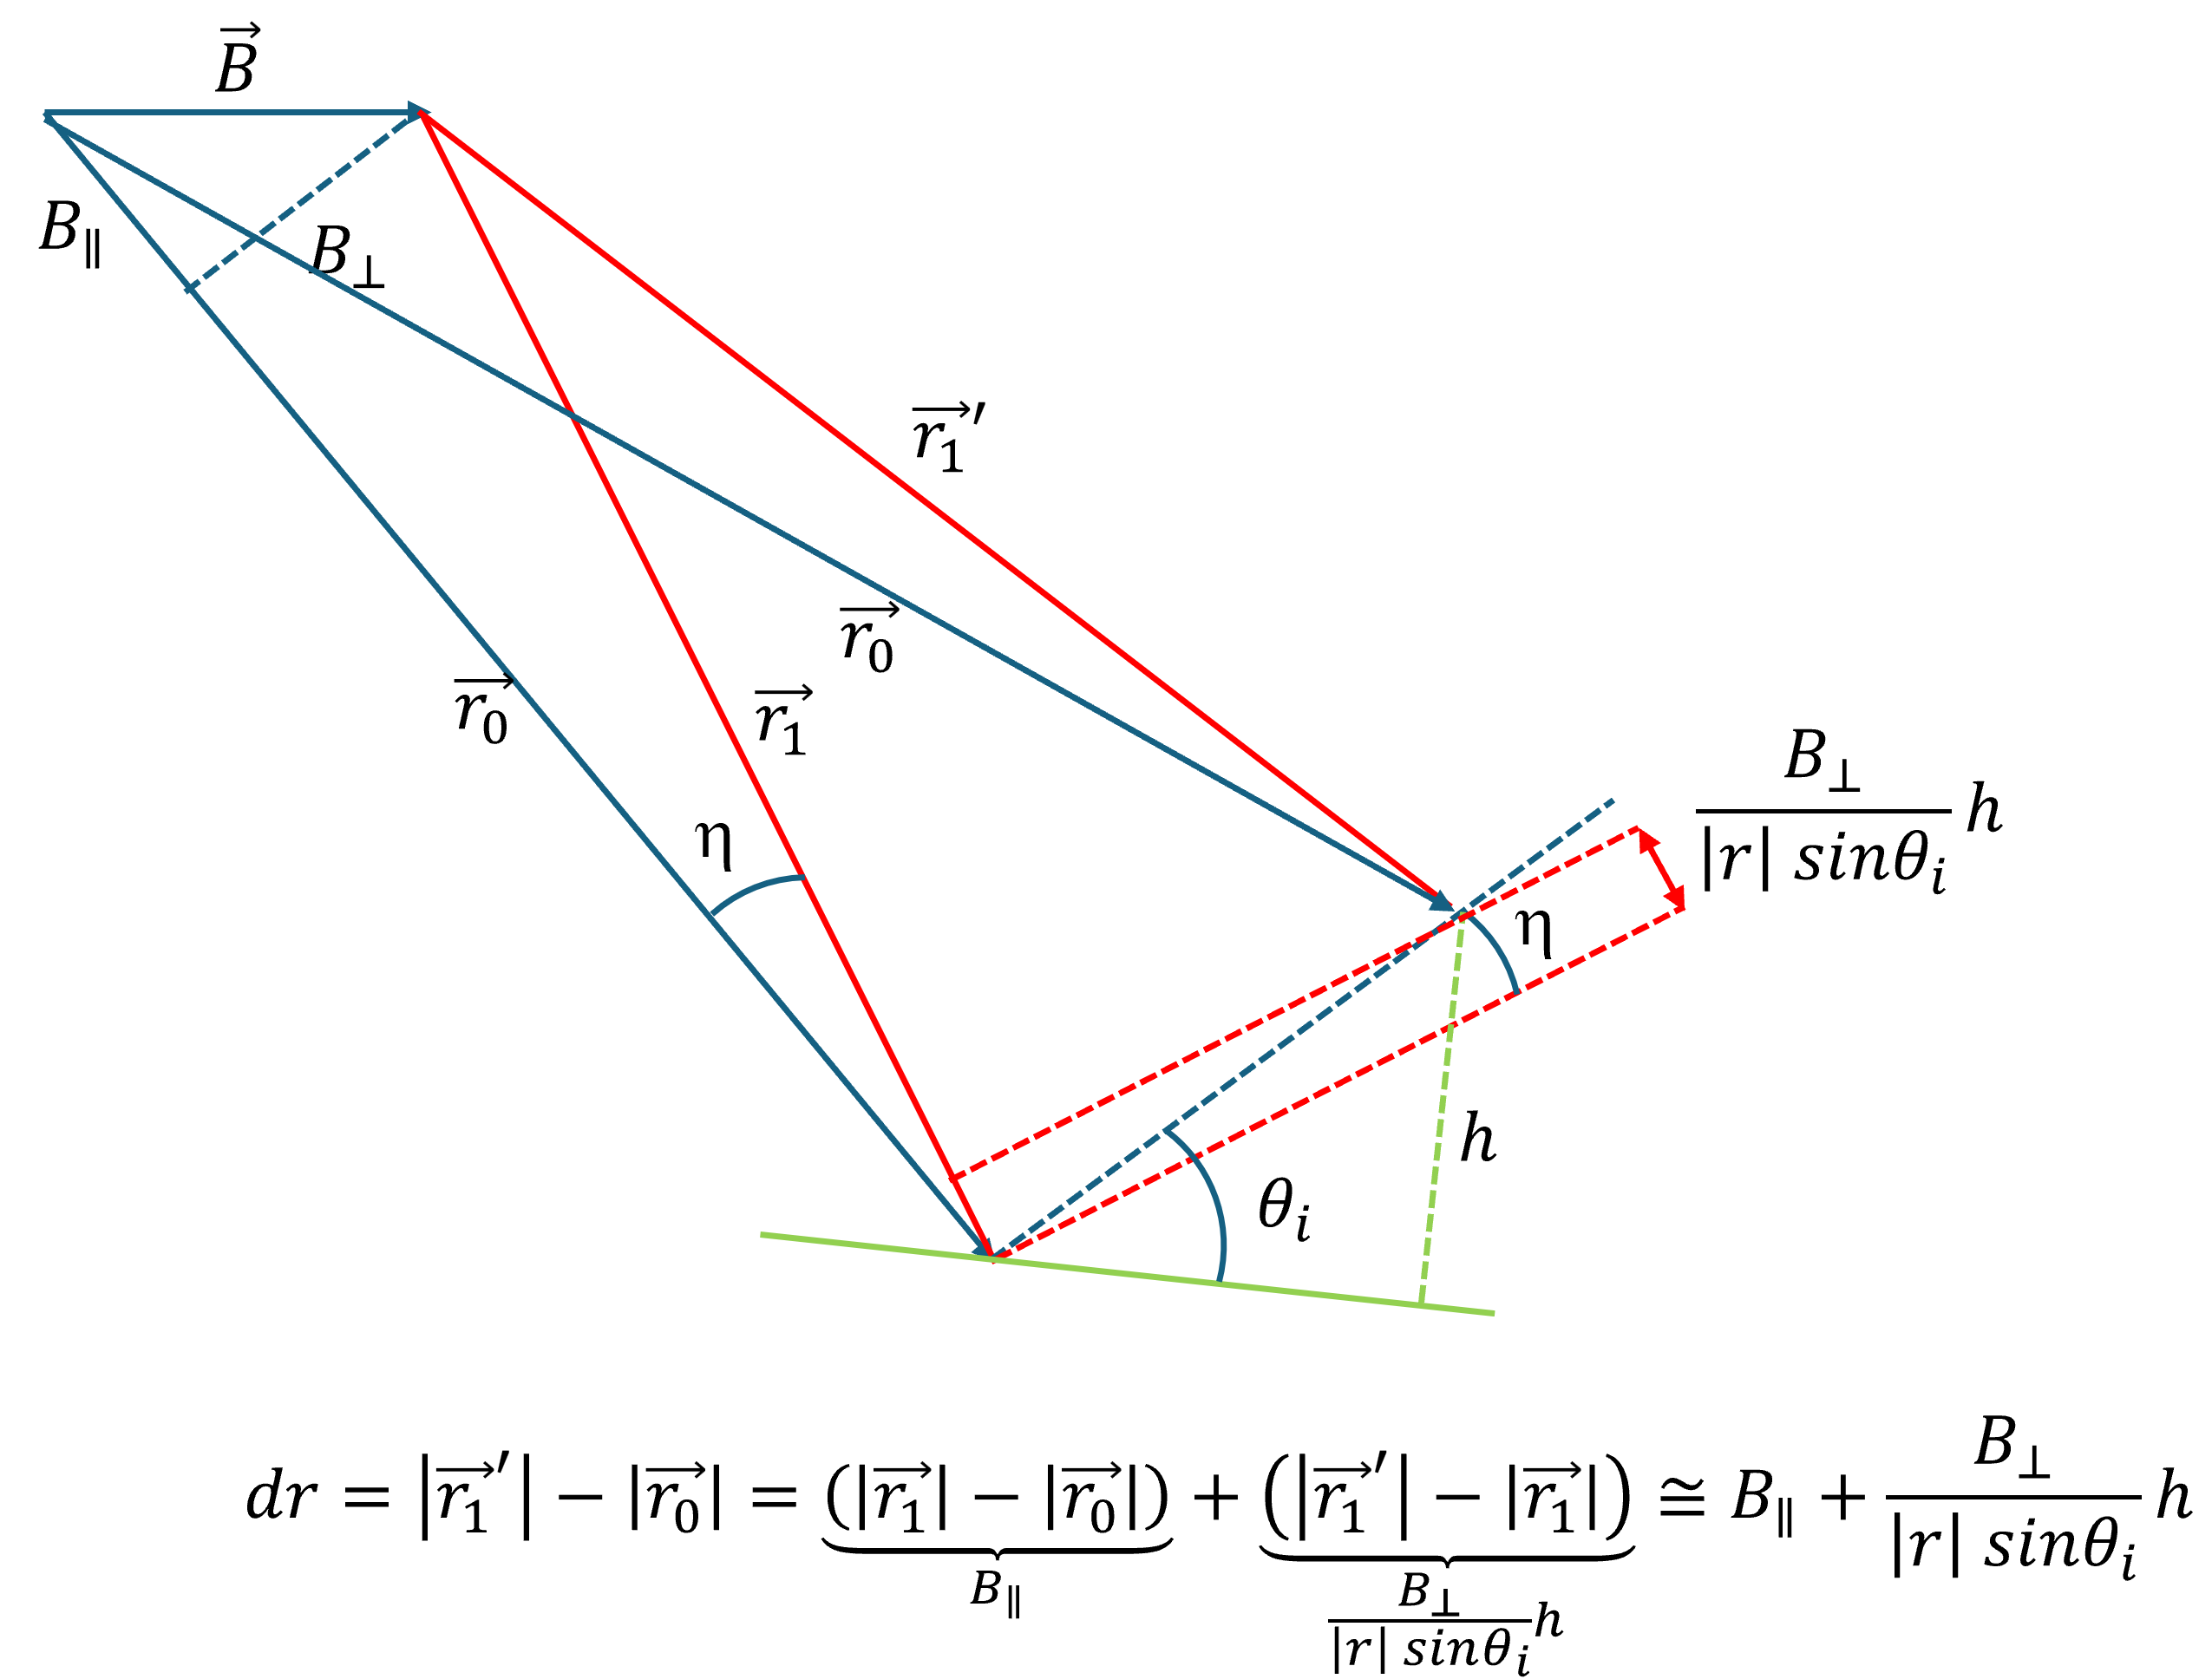
\includegraphics[width=0.9\textwidth]{Figures/cslc/dr_graph.png}
\caption{Simple sketch of the acquisition geometry. An error in the elevation of the target \(h\) implies an additional offset in range with respect to the difference in the satellite position in the line-of-sight of the reference image \(B_{\parallel}\).}
\label{fig:drg_from_dh}
\end{figure}

The standard deviation of the error in the slant-range position identification, denoted $\sigma_{dr}$, can be formulated as follows:

\begin{equation}
\sigma_{dr}^2 = \left(\frac{h}{R \sin\theta} \right)^2 \sigma_{B_{\perp}}^2 + \sigma_{B_{\parallel}}^2
\label{eq:slant_range_error_baseline}
\end{equation}

Here, $\sigma_{B_{\perp}}$ and $\sigma_{B_{\parallel}}$ represent the standard deviations of the perpendicular and parallel components, respectively, of the spatial baseline between the reference (master) and the secondary (slave) acquisition. The variables $h$, $R$, and $\theta$ correspond to the target height, slant-range distance, and incidence angle.

From equation~\ref{eq:slant_range_error_baseline}, it is evident that the first term is typically negligible in most scenarios. This is due to the fact that $h$ is generally on the order of a few kilometers, while $R \sin\theta$ is on the order of several hundred kilometers—thus significantly reducing the weight of the first term. Consequently, the dominant contribution to slant-range uncertainty is the uncertainty on the parallel component of the baseline, $\sigma_{B_{\parallel}}$.

This behavior is illustrated in Figure~\ref{fig:sigma_slant_range}, which shows the standard deviation in slant-range position $\sigma_{dr}$ (in meters) for various combinations of $(\sigma_{B_{\perp}}, \sigma_{B_{\parallel}}) \in \left[0, 0.25\right] \times \left[0, 0.25\right]$. As clearly shown, $\sigma_{dr}$ is most sensitive to variations in the parallel baseline uncertainty.

\begin{figure}[ht!]
\centering
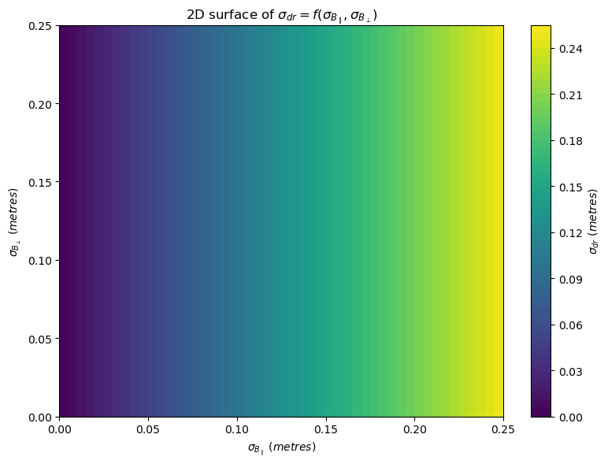
\includegraphics[width=0.9\textwidth]{Figures/cslc/sigma_slant_range.png}
\caption{Standard deviation in slant-range position $\sigma_{dr}$ (in meters) for each pair $(\sigma_{B_{\perp}}, \sigma_{B_{\parallel}}) \in \left[0, 0.25\right] \times \left[0, 0.25\right]$, assuming fixed parameters: $h = 1000$ m, $R = 600000$ m, and $\theta = 40^\circ$.}
\label{fig:sigma_slant_range}
\end{figure}

The error in azimuth position is determined by the zero-Doppler identification, which depends on the accuracy of the velocity vector. A simple sketch of the acquisition geometry is reported in Figure~\ref{fig:da_from_dv}.

\begin{figure}[ht!]
\centering
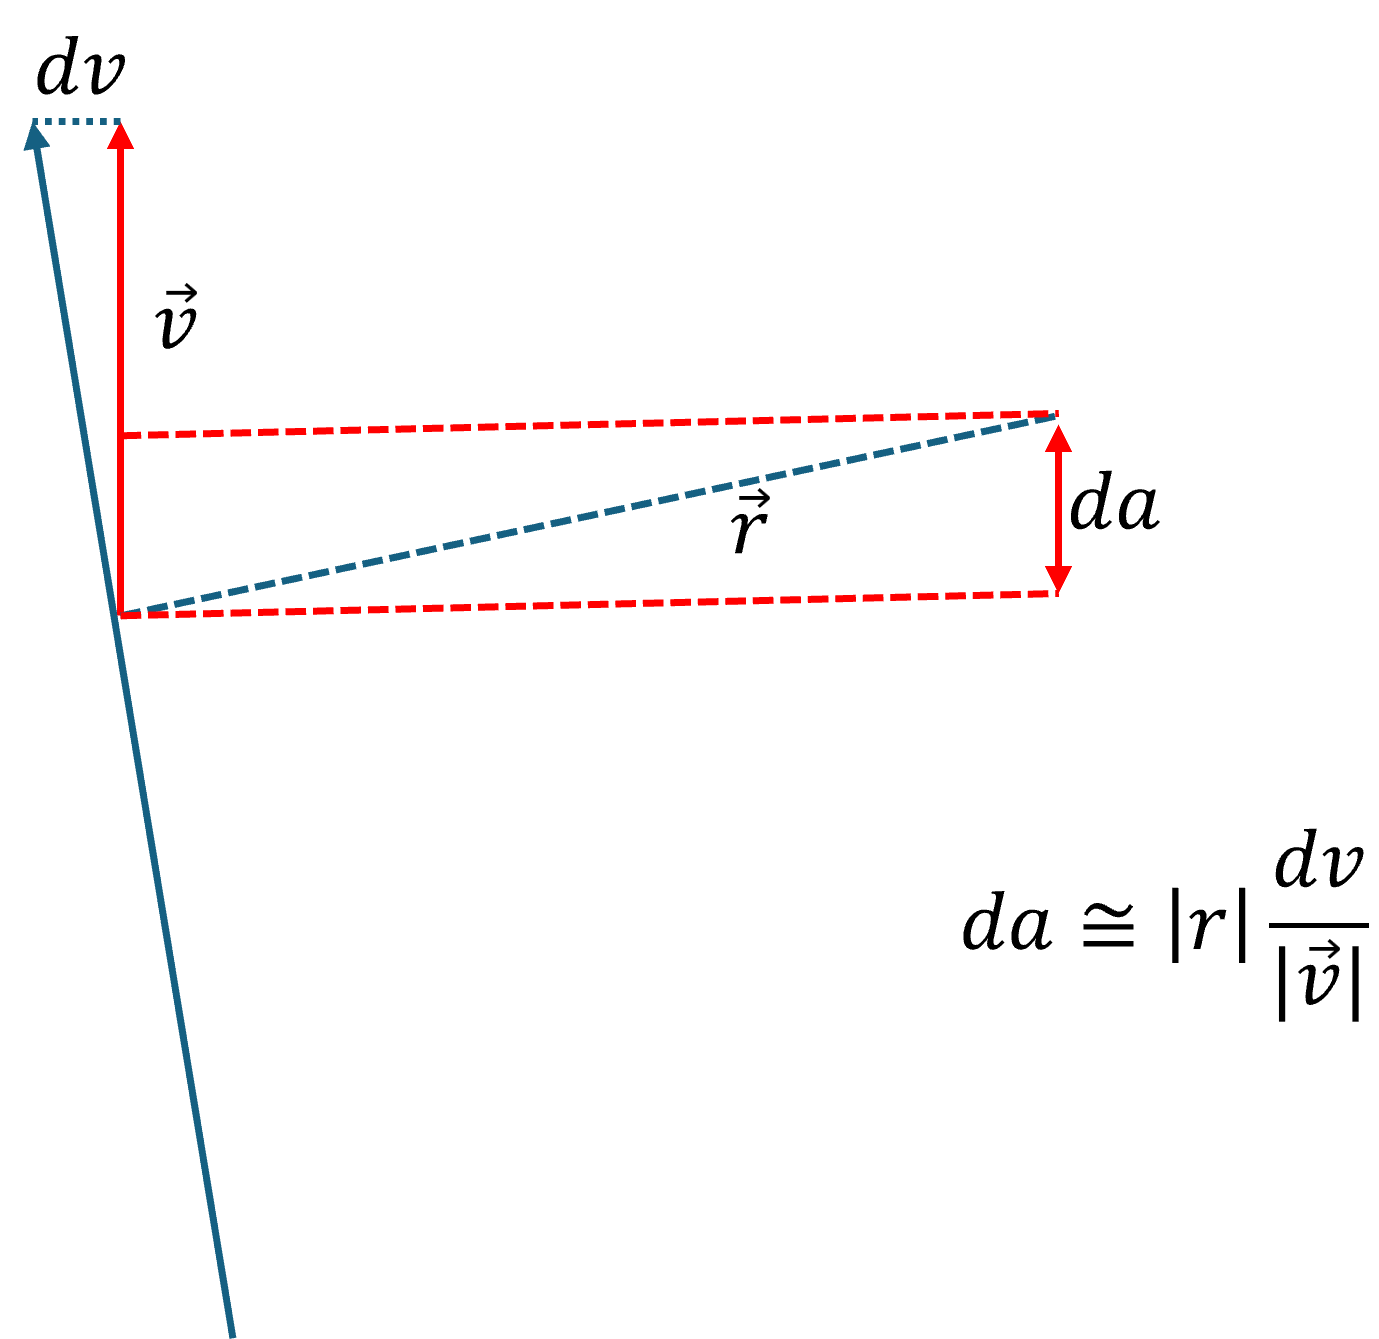
\includegraphics[width=0.4\textwidth]{Figures/cslc/da_graph.png}
\caption{Simple sketch of the acquisition geometry. An error in the velocity direction \(dv\) implies an error in the zero-Doppler determination.}
\label{fig:da_from_dv}
\end{figure}

The standard deviation of the error in azimuth position estimation, denoted $\sigma_{da}$, is given by:

\begin{equation}
\sigma_{da}^2 = \left( \frac{R}{\lVert \mathbf{v} \rVert} \right)^2 \sigma_{v_{\perp}}^2
\label{eq:azimuth_error_baseline}
\end{equation}

where $\lVert \mathbf{v} \rVert$ is the norm of the satellite velocity vector, and $\sigma_{v_{\perp}}$ is the standard deviation in the estimation of its perpendicular component with respect to the line-of-sight. Equation~\ref{eq:azimuth_error_baseline} shows that the azimuth error is directly proportional to $\sigma_{v_{\perp}}$.

This relationship is illustrated in Figure~\ref{fig:azimuth_error_baseline}, which shows the variation of $\sigma_{da}$ as a function of $\sigma_{v_{\perp}}$, assuming constant values of $R = 600000$ m and $\lVert \mathbf{v} \rVert = 7500$ m/s.

\begin{figure}[ht!]
\centering
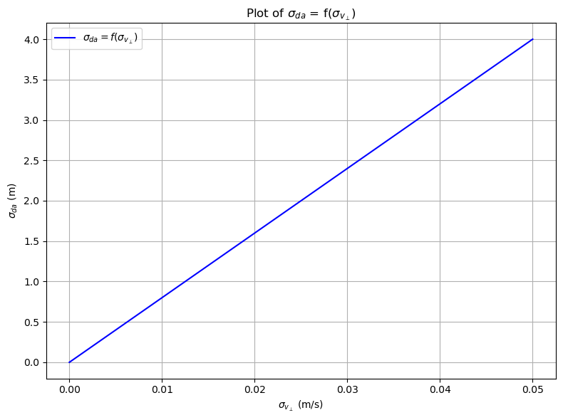
\includegraphics[width=0.9\textwidth]{Figures/cslc/sigma_azimuth.png}
\caption{Standard deviation in azimuth position $\sigma_{da}$ (in meters) as a function of the standard deviation in the perpendicular component of satellite velocity, $\sigma_{v_{\perp}}$, assuming $\lVert \mathbf{v} \rVert = 7500$ m/s and $R = 600000$ m.}
\label{fig:azimuth_error_baseline}
\end{figure}

An error in the input \acs{dem} primarily affects the slant-range positioning, with negligible impact on the azimuth direction. In particular, the standard deviation in slant-range position, $\sigma_{dr}$, previously derived in \ref{eq:slant_range_error_baseline}, must be increased with the following additional term to account for \acs{dem} height uncertainty:

\begin{equation}
\sigma_{dr}^2 = \left( \frac{B_{\perp}}{R \sin\theta} \right)^2 \sigma_{h}^2
\label{eq:eq_slant_range_error_dem}
\end{equation}

Here, $\sigma_{h}$ represents the standard deviation of the elevation error in the input \acs{dem}, and $B_{\perp}$ is the perpendicular component of the baseline between acquisitions. This term is linearly dependent on the height uncertainty, and thus highlights the sensitivity of slant-range accuracy to DEM quality.

Figure~\ref{fig:slant_range_error_dem} illustrates this relationship by showing the resulting $\sigma_{dr}$ values for varying $\sigma_{h}$, assuming $B_{\perp} = 1000$ m, $R = 600000$ m, and $\theta = 40^\circ$.

\begin{figure}[ht!]
\centering
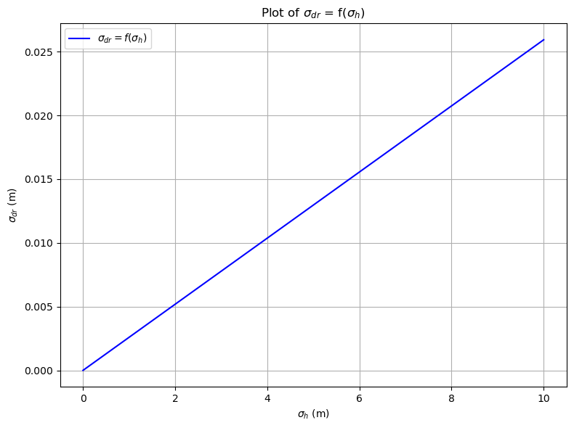
\includegraphics[width=0.9\textwidth]{Figures/cslc/sigma_slant_range_DEM.png}
\caption{Standard deviation in slant-range position $\sigma_{dr}$ (in meters) as a function of the standard deviation in the input \acs{dem} elevation, $\sigma_{h}$, assuming $B_{\perp} = 1000$ m, $R = 600000$ m, and $\theta = 40^\circ$.}
\label{fig:slant_range_error_dem}
\end{figure}

Under nominal conditions, orbital errors on the order of a few centimetres to decimetres and \acs{dem} inaccuracies of a few metres introduce only minor errors in the determination of the slant-range and azimuth positions of ground 3D coordinates. These sources of error can, to a first approximation, be considered negligible—particularly when compared to the significantly larger and more variable errors introduced by atmospheric propagation effects.

Among these, ionospheric and tropospheric delays represent the most prominent contributors. The ionospheric delay is dispersive, and thus strongly dependent on radar frequency. While its impact at C-Band is generally not so relevant (even if it is not completely negligible), it becomes a dominant source of slant range error at L-Band, where uncorrected distortions can exceed several meters—especially in equatorial regions or during periods of geomagnetic disturbance. 

Recent studies have quantified the residual co-registration error achievable with and without atmospheric compensation. Using Sentinel-1 C-band acquisitions over Chile, Zhang \textit{et al.} report an initial slant-range mis-registration \textit{RMSE} of \SI{0.20}{\metre} when only precise orbits and a \acs{dem} are applied; after model-driven corrections for ionosphere, troposphere, and solid-Earth tides, the error decreases to \SI{0.06}{\metre} (0.027 pixels), with 80 \% of scenes below \SI{0.07}{\metre}. In the companion L-band analysis, the uncorrected ALOS-2 stack shows an \textit{RMSE} of \SI{2.66}{\metre}; applying the same suite of atmospheric models reduces the error to \SI{0.56}{\metre}.


\begin{comment}
Our experiments with additional Sentinel-1 tracks (both ascending and descending) confirm the C-band figures: after the identical ionospheric, tropospheric, and tidal corrections, residual range offsets consistently fall in the \SIrange{0.05}{0.07}{\metre} interval—fully consistent with the published \SI{0.06}{\metre} value and well inside the \SI{0.1}{\metre} guideline adopted for ROSE-L quality assurance.  These results reinforce two key conclusions: (i) model-based atmospheric compensation is already sufficient for C-band interferometric applications, and (ii) additional refinement—particularly more accurate, low-latency TEC information—will be essential for meeting the stricter L-band accuracy targets foreseen for ROSE-L.  
HERE WE COULD INSERT THE RESULT IN TERMS OF COREGISTRATION ACCURACY WE HAVE USING AND NOT USING THE ETAD CASE SENTINEL-1
\end{comment}

Although the cited study maintains that the proposed model is sufficient to support image co-registration in interferometric applications, its direct extension to ROSE-L is not straightforward due to several key limitations:

\begin{itemize}
    \item The analysis does not consider azimuthal ionospheric effects, which can be as significant as range offsets in precise co-registration scenarios.
    
    \item The results are based on ALOS-2 acquisitions around 12:00 local solar time, a period typically associated with relatively mild ionospheric conditions. In contrast, \acs{rosel} is expected to acquire data near 18:00 local solar time, when ionospheric disturbances—particularly  at high latitudes (e.g., near the polar regions) or during periods of elevated solar activity—tend to be more severe. By extrapolating from ascending Sentinel-1 data (acquired at 18:00) and adjusting for the L-band wavelength scaling factor, an expected 1-sigma slant-range offset of approximately 1.6~m can be derived ($8.7~\text{cm} \times (\lambda_L/\lambda_C)^2$), which approaches the nominal slant-range resolution of \acs{rosel} (2.5~m). This level of error is too large to meet interferometric performance requirements.
    
    \item The study assumes a system bandwidth of 24~MHz, as used in the \acs{nisar} scenario. However, for \acs{rosel}'s standard mode (RIWS), the effective bandwidth may reach up to 60~MHz. This increases the sensitivity to range errors, thereby making \acs{rosel}’s ionospheric requirements significantly more stringent.
    
    \item Finally, the ionospheric correction performance in the referenced study relies on the use of JPL’s high-resolution ionosphere model (“JHR”), which is neither publicly available nor guaranteed in terms of latency or accessibility for operational processing pipelines.
\end{itemize}

All of these considerations must be carefully accounted for in the definition of co-registration and geolocation accuracy requirements. In particular, the requirements should be specified with respect to worst-case scenarios—such as acquisitions at high latitudes (e.g., polar regions) or during periods of elevated solar activity—where ionospheric disturbances are typically more severe. It is equally important to acknowledge that under more favorable conditions, such as acquisitions over equatorial or mid-latitude regions during geomagnetically quiet periods, significantly improved performance can be expected. In such cases, the achievable accuracy may exceed the baseline requirements by up to an order of magnitude.


To verify that the theoretical error budget presented here is achievable in practice, we performed a dedicated co-registration experiment using a Sentinel-1 image stack acquired over the Surat Basin, Australia, where a network of calibrated corner reflectors (CRs) is permanently installed.  All CRs with radar-cross-section \(>\) 35 dBsm were retained as control targets. Two sets of \acs{cslc}s were generated with respect to a single master \acs{slc}:  
\begin{itemize}
    \item using only precise orbits and the 30 m SRTM DEM;   
    \item unsing also the \acs{etad} layers were additionally applied to compensate tropospheric and ionospheric delays.
\end{itemize}

For every slave image and for each visible CR, the residual offset vector \(\Delta r\) (slant range) and \(\Delta a\) (azimuth) was measured as the sub-pixel displacement between the CR’s peak position in the master and in the resampled slave.  Sub-pixel locations were estimated by oversampling (with a sinc interpolator) both master and co-registered slave in corrispondence on the CR response.

Figure~\ref{fig:delta_coreg_before_etad} shows the accuracy achieved using only orbital and DEM information, while Figure~\ref{fig:delta_coreg_after_etad} presents the results obtained when \acs{etad} corrections are included in the co-registration process.

In both figures, the $x$-axis lists the identifiers of the corner reflectors (CRs) used in the analysis, and the $y$-axis reports the measured mis-registration in slant range (left) and azimuth (right), both expressed in metres.
Each dot represents the residual offset for a single CR; different colours correspond to different slave images co-registered to the same master.

By comparing the two plots, it becomes evident that atmospheric delays—although modest at C-band—introduce a systematic error in slant range when not corrected.
In Figure~\ref{fig:delta_coreg_before_etad}, each slave shows a distinct mean offset in range, visible as a vertical shift across CRs of the same colour. This is consistent with the slow spatial variability of tropospheric and ionospheric delays, which act primarily as a constant bias in slant range.
The azimuth direction is less affected, showing minimal variation in both mean and spread.

When \acs{etad} information is used (Figure~\ref{fig:delta_coreg_after_etad}), this systematic range bias is significantly reduced, aligning the mean residuals closer to zero.
While the standard deviation (i.e., the random component) remains nearly unchanged, the correction of the constant bias enhances absolute co-registration accuracy.
This confirms that—even at C-band—accounting for atmospheric delays improves product consistency, particularly in applications requiring high geometric precision.

\begin{figure}[ht!]
\centering
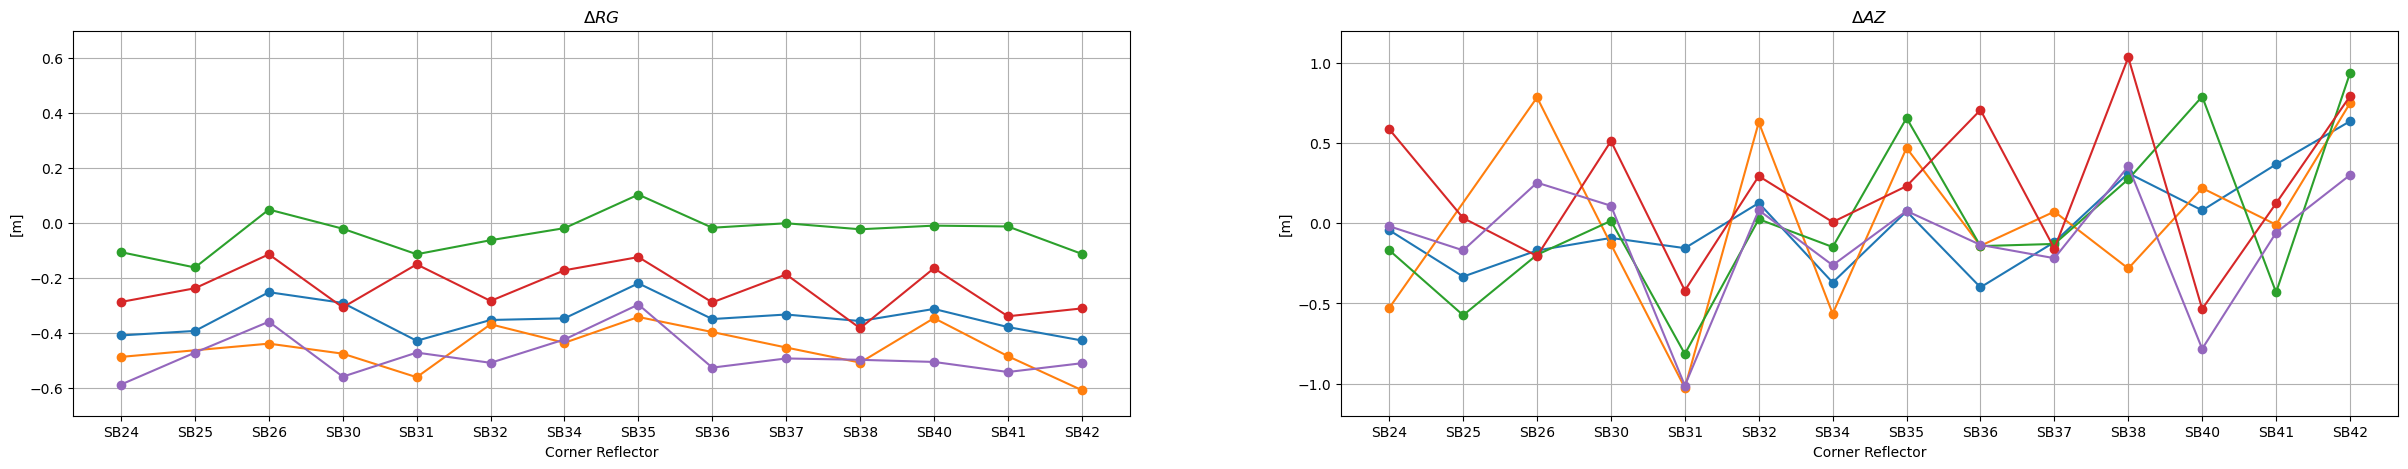
\includegraphics[width=0.9\textwidth]{Figures/cslc/delta_coreg_before_etad.png}
\caption{Co-registration errors using only orbital and DEM information. Each dot shows the mis-registration (in metres) of a corner reflector in slant range (left) and azimuth (right). Colours indicate different slave images.}
\label{fig:delta_coreg_before_etad}
\end{figure}


\begin{figure}[ht!]
\centering
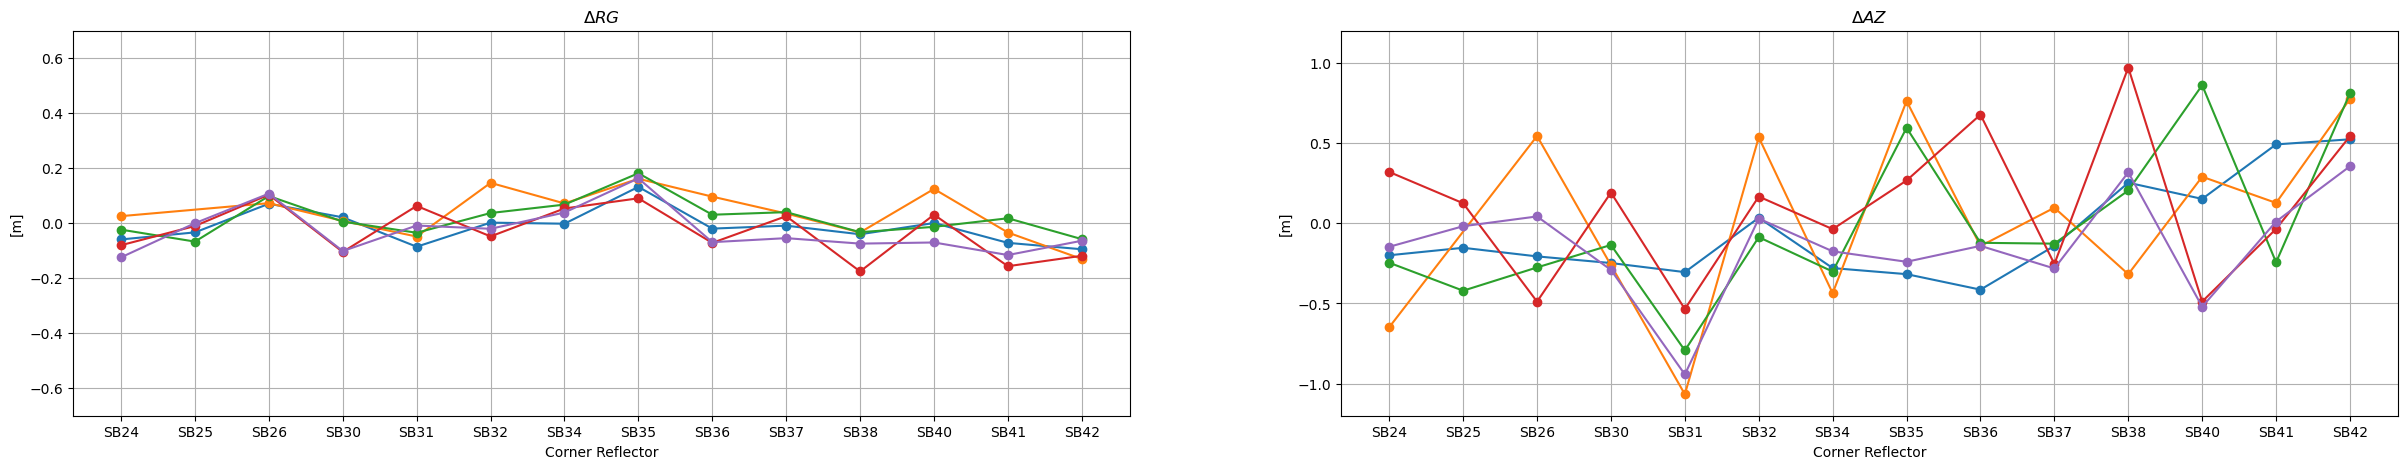
\includegraphics[width=0.9\textwidth]{Figures/cslc/delta_coreg_after_etad.png}
\caption{Co-registration errors using orbital, DEM, and ETAD information. The systematic range bias visible in Figure~\ref{fig:delta_coreg_before_etad} is largely corrected. The azimuth alignment remains stable in both cases.}
\label{fig:delta_coreg_after_etad}
\end{figure}
In the Co-registration, the following parameters have been used:
\begin{itemize}
    \item warp\_ov\_fact, number of samples used to generate the sinc function: 100000
    \item warp\_kernel\_shape, shape of the interpolation kernel (height, width): [11,11]
    \item warp\_kaiser\_beta, beta parameter for the Kaiser window used to weight the sinc function: 6
\end{itemize}

\subsubsection{Absolute geolocation accuracy}
\label{sec:gslc_absolute_geolocation_accuracy}

In order to evaluate the absolute geolocation accuracy of the projected product (\acs{gslc}), the following elements must be considered: the vertical and horizontal accuracy of the \acs{dem}, and the accuracy in determining the range and azimuth coordinates in the \acs{slc} images. The relationship linking geolocation accuracy with input data accuracy, in the zero-Doppler plane, can be explained starting from the acquisition geometry sketch shown in Figure~\ref{fig:gslc_geolocation_accuracy}.

\begin{figure}[ht!]
\centering
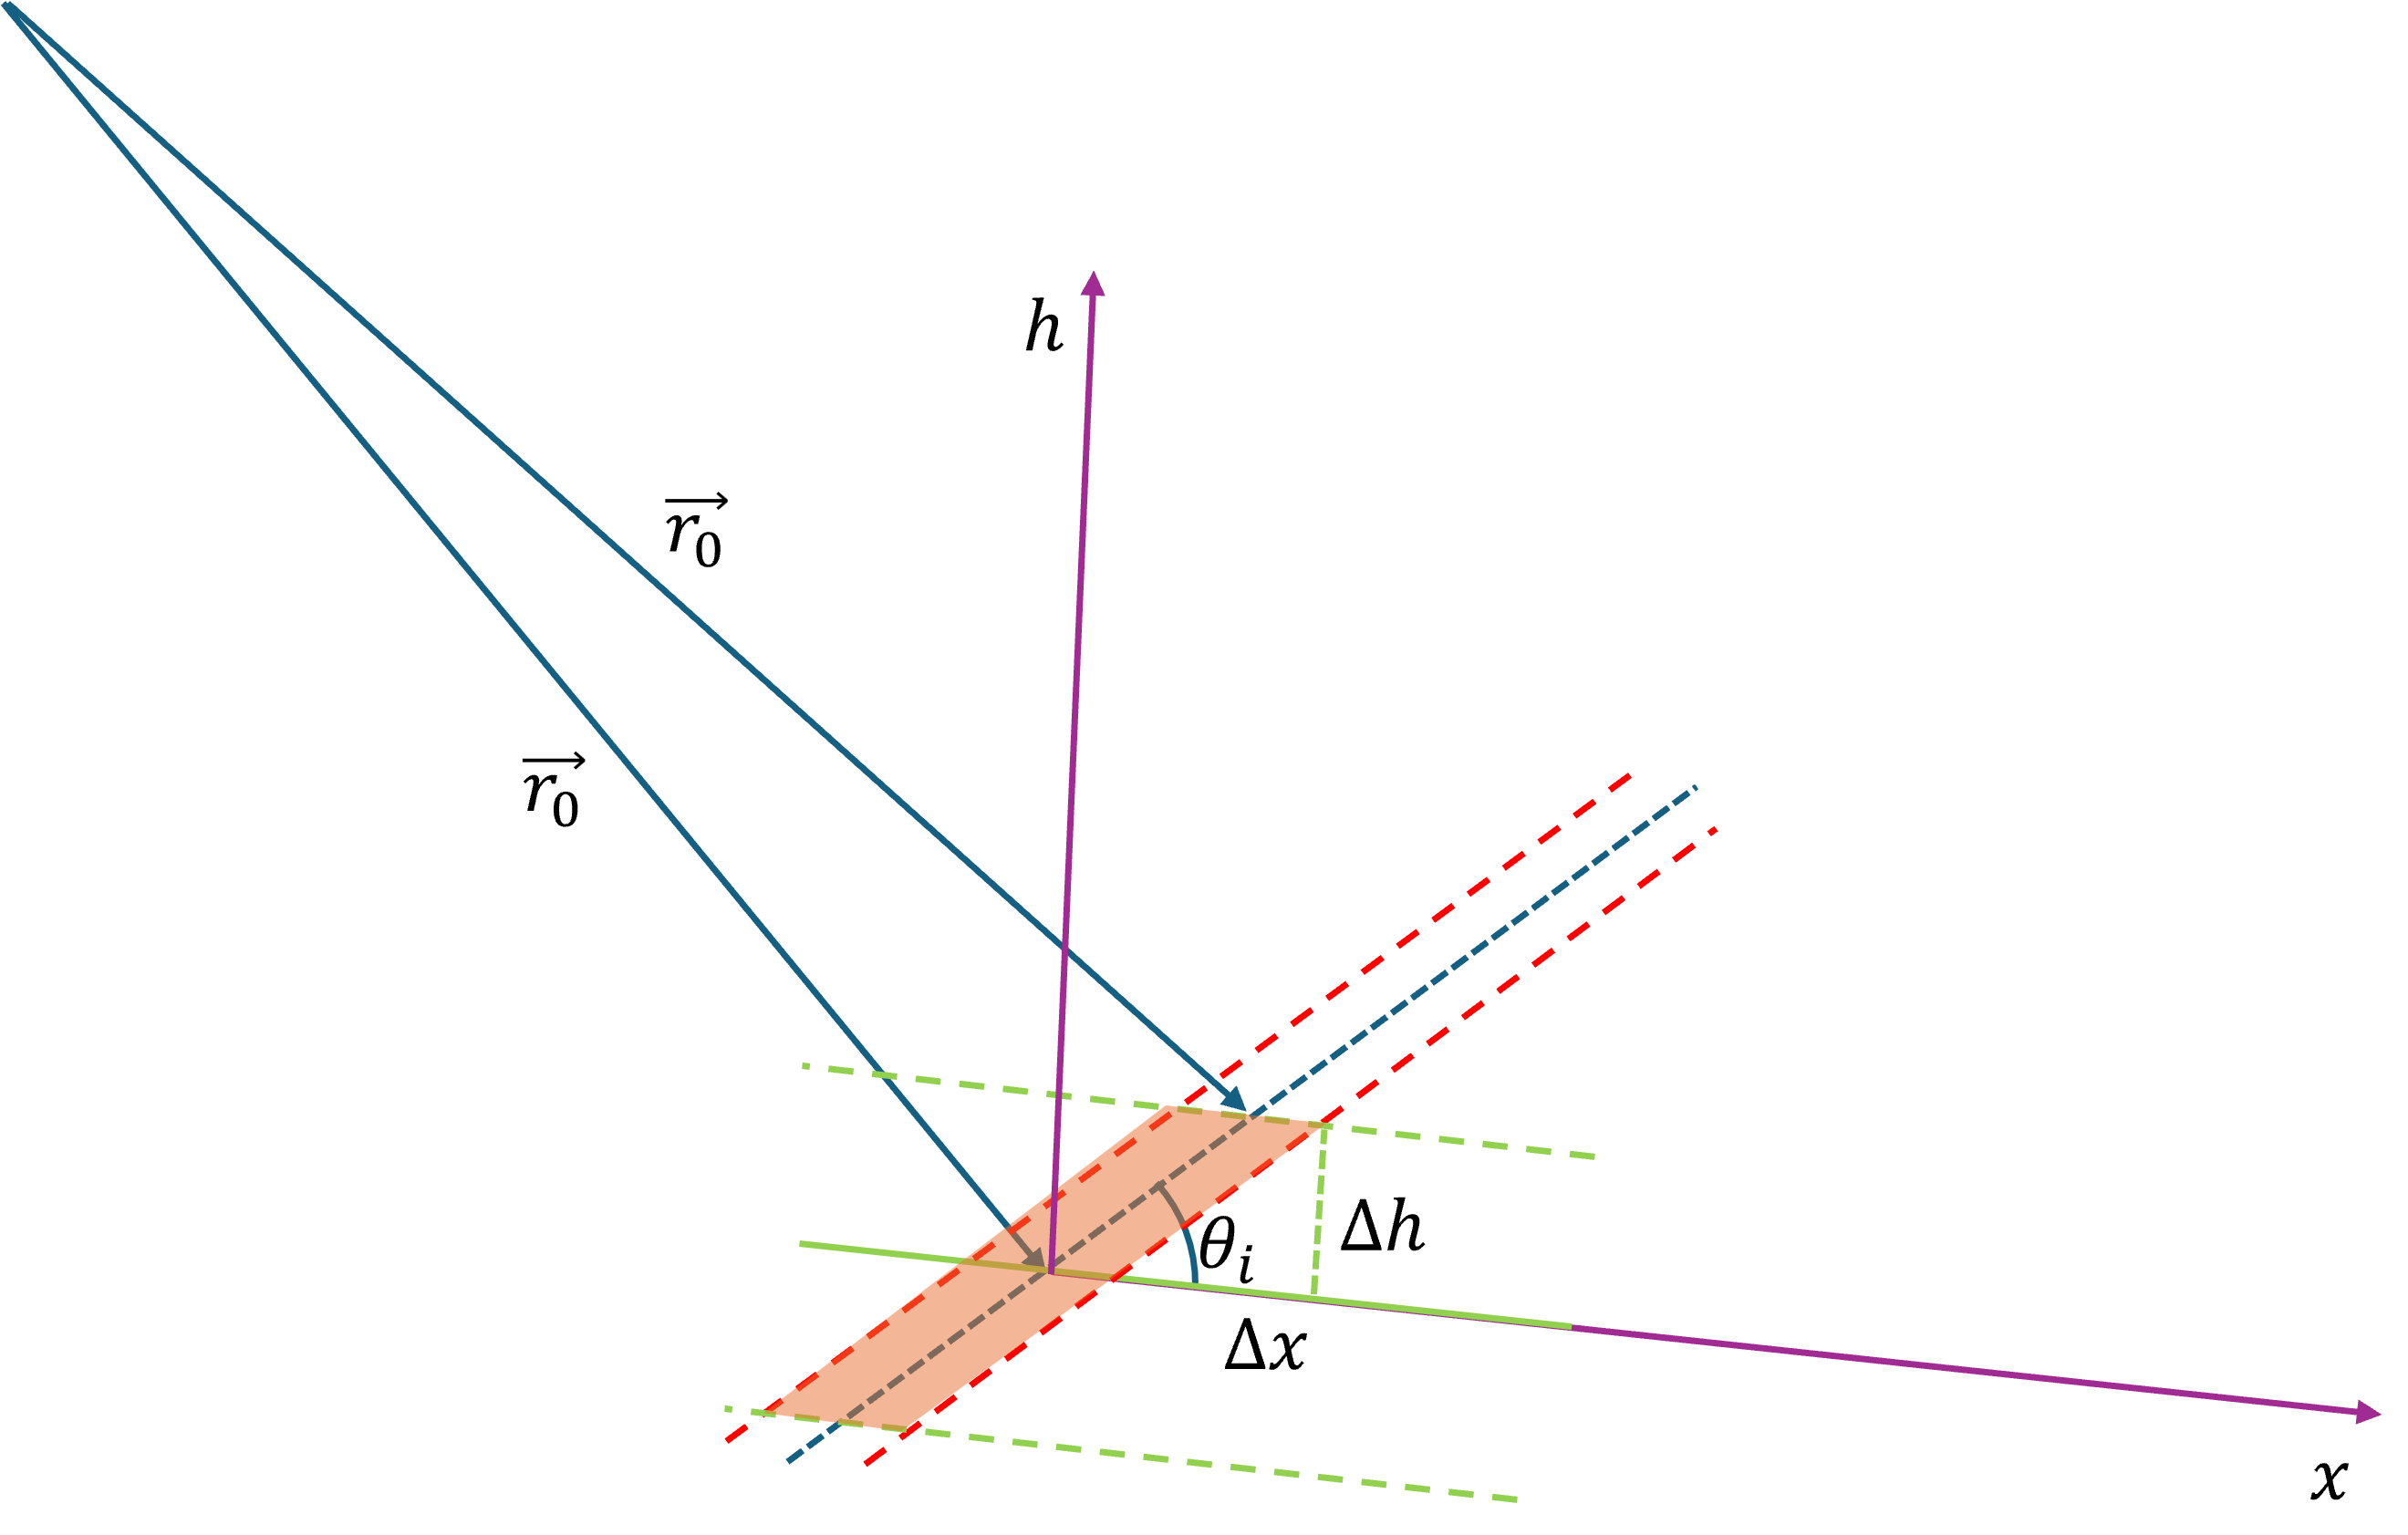
\includegraphics[width=0.9\textwidth]{Figures/cslc/geolocation_accuracy.png}
\caption{Simplified sketch of the acquisition geometry of a single SAR image in the zero-Doppler plane. The localization error of a ground point results from the combined uncertainty in the slant-range position and the \acs{dem} surface.}
\label{fig:gslc_geolocation_accuracy}
\end{figure}

The area where the point can be geolocated is constrained by the error in slant-range position (red dashed lines) and the error in elevation (green dashed lines).  
Let $\alpha$ be the local slope, $\theta_i$ the local incidence angle, $\sigma^{DEM}_x$ and $\sigma^{DEM}_h$ the horizontal and vertical accuracy of the input \acs{dem}, and $\sigma_{dr}$ the slant-range accuracy of the input \acs{slc}. The final error in the $x$ coordinate is given by:

\begin{equation}
\sigma_{dx}^2 = \frac{\sigma^2_h}{\tan^2 \theta_i} + \frac{\sigma^2_{dr}}{\sin^2 \theta_i} = \frac{\left(\sigma^{DEM^2}_x \tan^2 \alpha + \sigma^{DEM^2}_h\right)}{\tan^2 \theta_i} + \frac{\sigma^2_{dr}}{\sin^2 \theta_i}
\label{eq:gslc_dx_accuracy}
\end{equation}

When ETAD corrections are applied, the error in slant-range position is reduced to a few centimeters, both in terms of bias and standard deviation. Therefore, the second term (slant-range) in Equation~\ref{eq:gslc_dx_accuracy} becomes negligible compared to the first term (\acs{dem}), which is typically one order of magnitude larger. Without ETAD corrections, both sources of error are comparable and typically on the order of few meters.

\subsubsection{Radiometric quality}
\label{sec:cslc_radiometric_quality}

The evaluation of radiometric fidelity for the \acs{cslc} product is theoretically grounded in the analysis of key image quality indicators, namely Spatial Resolution, Peak Side-Lobe Ratio (\acs{pslr}), and Integrated Side-Lobe Ratio (\acs{islr}). These metrics are derived from the impulse response of point scatterers and provide insight into the integrity of the SAR signal following resampling.

In the generation of \acs{cslc} products, co-registration is achieved by interpolating the slave image to the master’s geometry. This process uses a finite-length sinc interpolator modulated by a Kaiser window. The sinc kernel, by design, preserves the frequency content of the original signal, ensuring minimal degradation in spatial resolution. The Kaiser window serves to suppress the side lobes of the interpolator's response, thereby mitigating increases in \acs{pslr} and \acs{islr}.

Theoretically, such an interpolation strategy is expected to introduce very limited radiometric degradation. Provided the interpolation kernel is sufficiently long and well-parameterized, the resulting \acs{cslc} product should retain the spatial and radiometric quality of the input \acs{slc} data with negligible impact.

This expectation is supported by standard SAR signal processing literature, which demonstrates that sinc interpolation with appropriate windowing results in minimal loss of resolution and side-lobe performance \cite{Cumming2005}, \cite{Moreira2013}, \cite{Soumekh1999}. Accordingly, any deviations observed in practice are more likely attributable to implementation or data-specific effects rather than inherent limitations of the resampling approach. 

To assess the impact of the co-registration process on radiometric quality, the differences in Integrated Side-Lobe Ratio (\acs{islr}) and Peak Side-Lobe Ratio (\acs{pslr}) between co-registered \acs{slc} products (\acs{cslc}) and their original \acs{slc} counterparts were computed. These differences are visualized in Figures~\ref{fig:PSLR_comparison} and~\ref{fig:ISLR_comparison}, using a comprehensive set of Corner Reflectors (\acs{cr}s) with Radar Cross Sections exceeding 35 dBsm. 

For each CR and for each image pair (original and co-registered), \acs{islr} and \acs{pslr} were estimated independently in both the slant-range and azimuth directions. The x-axis of each plot shows the original metric value as measured on the \acs{slc}, while the y-axis shows the corresponding difference observed after co-registration. 

Each dot represents an individual CR; dots sharing the same color refer to CRs measured within the same image. Color changes denote a change in the input \acs{slc} scene. This visualization enables the detection of systematic biases or degradations introduced by the co-registration step and confirms the expected minimal impact on radiometric sharpness indicators.

\begin{figure}[h!]
\centering
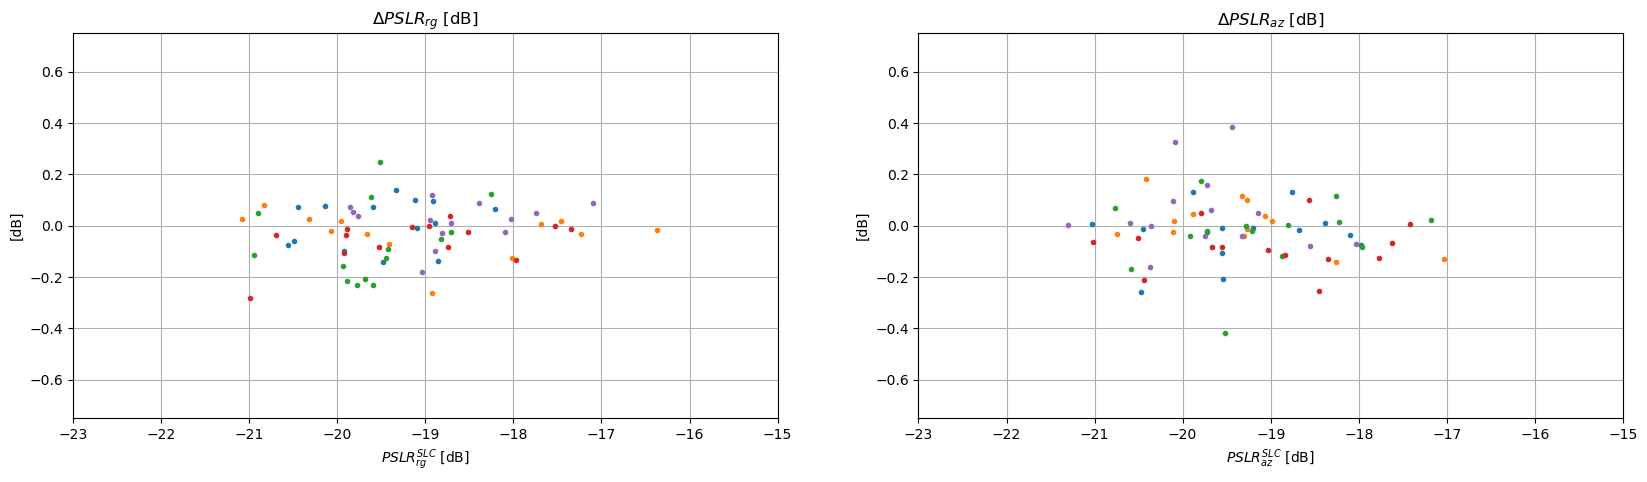
\includegraphics[width=0.9\textwidth]{Figures/cslc/PSLR_comparison.png}
\caption{Difference in Peak Side-Lobe Ratio (\acs{pslr}), expressed in dB, between co-registered \acs{slc} products (\acs{cslc}) and their original \acs{slc} counterparts. The left panel shows the \acs{pslr} difference in slant-range direction, while the right panel shows the difference in azimuth. The x-axis represents the original \acs{pslr} value (in dB) as measured on the \acs{slc}, and the y-axis shows the difference $\text{PSLR}^{\text{CSLC}} - \text{PSLR}^{\text{SLC}}$. Each dot corresponds to a single Corner Reflector (\acs{cr}) with Radar Cross Section (\acs{rcs}) greater than 35 dBsm. Dots of the same color refer to \acs{cr}s within the same image; changes in color indicate different \acs{slc}.}
\label{fig:PSLR_comparison}
\end{figure}

\begin{figure}[h!]
\centering
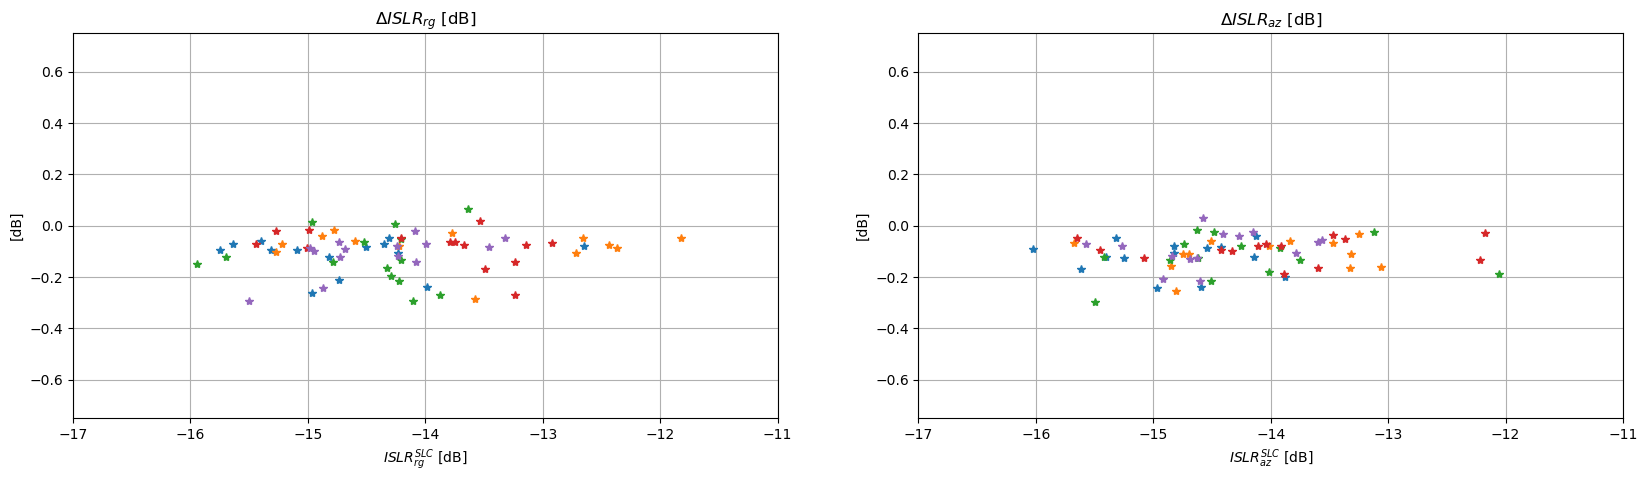
\includegraphics[width=0.9\textwidth]{Figures/cslc/ISLR_comparison.png}
\caption{Difference in Integrated Side-Lobe Ratio (\acs{islr}), expressed in dB, between co-registered \acs{slc} products (\acs{cslc}) and their original \acs{slc} counterparts. The left panel shows the \acs{islr} difference in slant-range direction, while the right panel shows the difference in azimuth. The x-axis represents the original \acs{islr} value (in dB) as measured on the \acs{slc}, and the y-axis shows the difference $\text{ISLR}^{\text{CSLC}} - \text{ISLR}^{\text{SLC}}$. Each dot corresponds to a single Corner Reflector (\acs{cr}) with Radar Cross Section (\acs{rcs}) greater than 35 dBsm. Dots of the same color refer to \acs{cr}s within the same image; changes in color indicate different \acs{slc}.}
\label{fig:ISLR_comparison}
\end{figure}

In addition to \acs{islr} and \acs{pslr}, the potential impact of co-registration on spatial resolution was assessed. Figure~\ref{fig:spatial_resolution_comparison} presents the resolution difference, expressed in meters, between the co-registered \acs{slc} (\acs{cslc}) and the original \acs{slc}, evaluated separately in slant-range (left panel) and azimuth (right panel) directions.

The x-axis in each panel reports the spatial resolution measured on the original \acs{slc} product, while the y-axis shows the corresponding resolution difference after co-registration. As with the previous figures, each point corresponds to a single \acs{cr} (\acs{rcs} > 35 dBsm), and colors are used to distinguish \acs{cr}s across different \acs{slc} scenes.

The plots confirm that spatial resolution remains stable across all analyzed scenes and directions, further supporting the conclusion that the applied co-registration method introduces negligible degradation in radiometric sharpness and point target response.

\begin{figure}[h!]
\centering
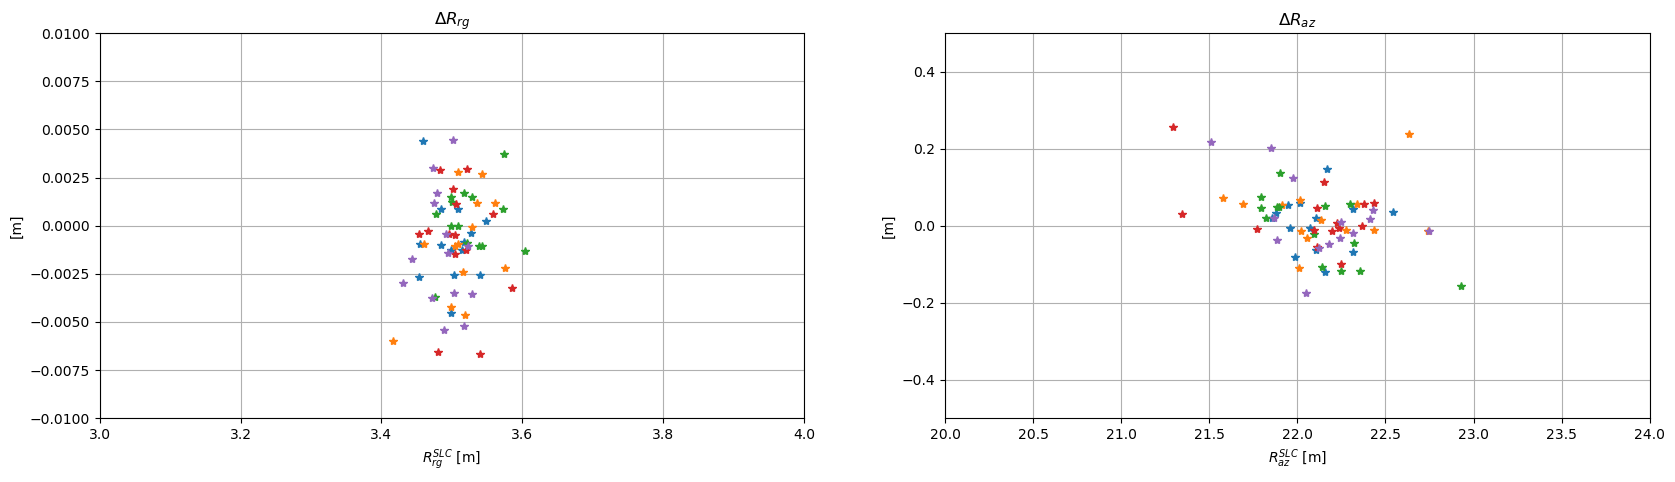
\includegraphics[width=0.9\textwidth]{Figures/cslc/spatial_resolution_comparison.png}
\caption{Difference in spatial resolution (in metres) between the co-registered \acs{slc} product (\acs{cslc}) and the original \acs{slc}. The left panel shows the difference in slant-range resolution, and the right panel in azimuth resolution. The x-axes report the original spatial resolution of the \acs{slc} product in each direction. Each point corresponds to a Corner Reflector with \acs{rcs} greater than 35 dBsm. As in previous figures, dots of the same color indicate \acs{cr}s extracted from the same image, while color changes correspond to different input \acs{slc} scenes.}
\label{fig:spatial_resolution_comparison}
\end{figure}

\begin{figure}[h!]
\centering
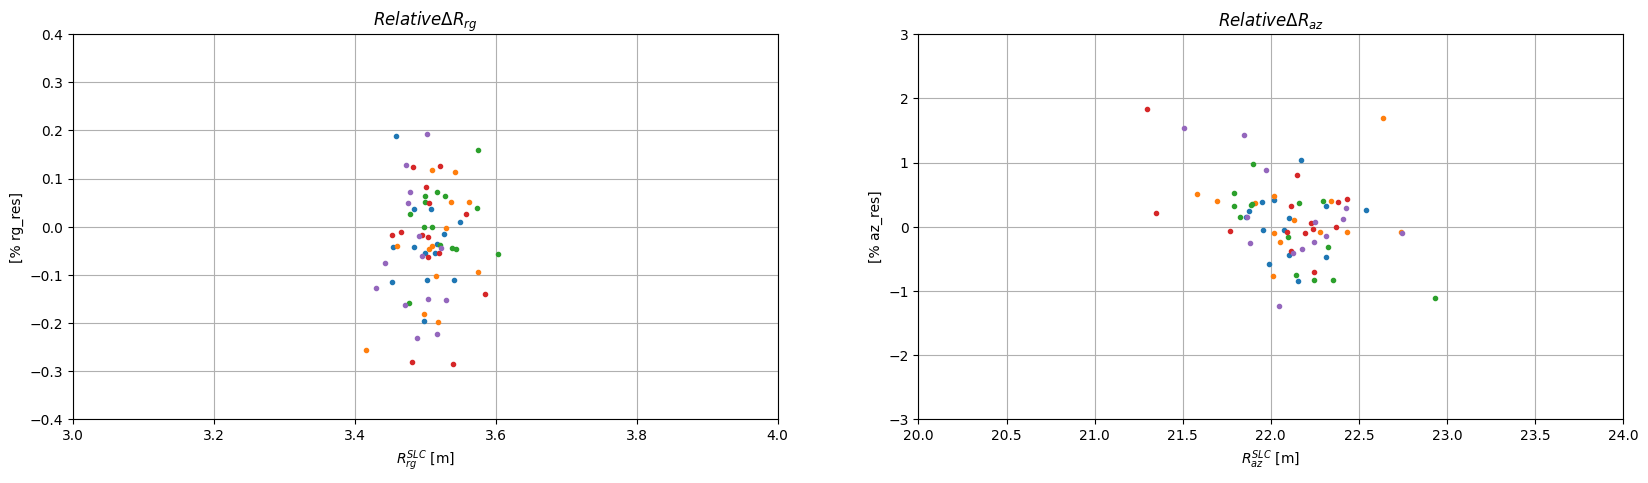
\includegraphics[width=0.9\textwidth]{Figures/cslc/spatial_resolution_comparison_relative.png}
\caption{Relative difference in spatial resolution (percentage with respect to the satellite resolution) between the co-registered \acs{slc} product (\acs{cslc}) and the original \acs{slc}. The left panel shows the difference in slant-range resolution, and the right panel in azimuth resolution. The x-axes report the original spatial resolution of the \acs{slc} product in each direction. Each point corresponds to a Corner Reflector with \acs{rcs} greater than 35 dBsm. As in previous figures, dots of the same color indicate \acs{cr}s extracted from the same image, while color changes correspond to different input \acs{slc} scenes.}
\label{fig:spatial_resolution_comparison_relative}
\end{figure}


The theoretical framework for evaluating the radiometric fidelity of the \acs{gslc} product follows similar principles to those applied for the \acs{cslc}. In particular, the geocoding process employs a finite-length sinc interpolator modulated by a Kaiser window, which is theoretically well-suited to preserving signal integrity. This approach ensures minimal degradation of the original \acs{sar} signal, particularly when the ground sampling interval is chosen to match the nominal resolution of the sensor as closely as possible.

However, unlike the \acs{cslc}, the transformation from radar to ground coordinates introduces additional challenges that could affect the radiometric quality indicators. In particular:

\begin{itemize}
    \item \textbf{Topographic distortion effects}: Elevation variation causes geometric distortions such as foreshortening, layover, and shadowing in the geocoded image, which can degrade the shape and sharpness of point target responses.
    \item \textbf{Geolocation-induced rotation}: The projection from radar to geographic coordinates results in a rotation of the image grid, misaligning the slant-range and azimuth directions with the map axes. This can distort the impulse response function, making resolution and side-lobe measurements less consistent.
    \item \textbf{\acs{dem} dependency}: The accuracy of the geocoding process depends heavily on the quality of \acs{dem}. Errors in the \acs{dem} can lead to geometric misregistration, signal smearing, and local inaccuracies.
\end{itemize}

As a consequence, while the theoretical interpolation scheme remains robust, these secondary effects can lead to measurable degradation in image quality indicators such as Spatial Resolution, \acs{islr}, and \acs{pslr}. Furthermore, the geometric transformations applied during geocoding make it more complicated to obtain a reliable estimate of these indicators.

Therefore, these considerations should be reflected in the product specifications used to assess whether the geocoding process has been implemented correctly and within acceptable tolerances. 



\subsection{Computational performance}
\label{sec:cslc_computation}

\subsubsection{Co-registration Workflow}

The computational load of co-registering a slave image to a master grid is dominated by three successive operations.

\paragraph{\acs{dem} to radar coordinate conversion}  
Processing begins by mapping every node of the Digital Elevation Model (\acs{dem}) covering the Area Of Interest (AOI) into radar coordinates.  
For each \acs{dem} triplet $(x,y,z)$ the algorithm solves the range–Doppler equations to obtain the slant-range distance $r$ and the zero-Doppler azimuth time $t$.  
Because the system is non-linear, an iterative Newton–Raphson search is required, typically converging in five to eight iterations.  
Hence the cost grows linearly with the number of \acs{dem} nodes, $K\!\propto\!\text{AOI}/\Delta_{\text{DEM}}^{2}$.  
For example, a 100 km × 100 km scene sampled at 30 m already involves $\sim$11 million DEM points.

\paragraph{Interpolation of the sparse control mesh}  
The resulting tie points $\{(r_i,t_i)\}$ form an irregular control mesh that must be interpolated onto the master’s regular radar grid.  
A common strategy is to build a Delaunay triangulation (cost $\mathcal{O}(K\log K)$) and then apply barycentric interpolation; each master pixel is evaluated in constant time with three multiplications and two additions.


\paragraph{Image warping with a sinc–Kaiser kernel}  
Finally, the slave signal is resampled onto the master grid.  
For every output pixel the algorithm evaluates a finite two-dimensional sinc kernel apodised by a Kaiser window.  
With an \(M\times N\) kernel the operation count is \(MN\) multiplications plus \(MN-1\) additions per pixel; high-fidelity implementations typically use a kernel of at least \(11\times11\).

\bigskip
\noindent
In summary, the DEM projection cost scales with AOI size and DEM spacing, while the warping stage scales with the number of output pixels and the chosen kernel width.  Exploiting multi-core CPUs or GPUs is therefore essential for wide-swath, high-resolution production environments.

\paragraph{Optional cross–correlation refinement}  
When orbit and \acs{dem} information alone are insufficient to guarantee sub-pixel alignment (and there are not any other auxiliary data to be used to improve the co-registration accuracy), an image-based refinement is applied on a sparse grid of control patches. This refinement can use either frequency-domain spectral diversity or spatial cross-correlation. For the latter, small window pairs (e.g.\ $64\times64$ pixels) are extracted at regular spacing and matched to estimate residual offsets.

Implementing cross-correlation requires an additional processing loop:  
\begin{itemize}
\item a coarse-warp of the slave image based solely on geometric information;  
\item cross-correlation of the coarse-warped slave against the master to update the correspondence map; and  
\item a fine-warp using the refined offsets.  
\end{itemize}
This strategy effectively doubles the computational cost of the sinc–Kaiser warp, yet it is often indispensable for achieving the sub-pixel co-registration accuracy demanded by high-coherence interferometry.

\subsubsection{Geocoding Workflow}

Geocoding—the mapping of radar samples onto a ground-projected grid—shares two of the three co-registration steps.

\paragraph{Ground-grid definition and DEM projection}  
A regular ground lattice \((X,Y)\) (e.g.\ UTM or UPS) is first defined at the desired posting, typically chosen close to the native radar resolution.  The height of each ground node, \(h(X,Y)\), is obtained by bilinear or bicubic interpolation of the \acs{dem}.  Each 3-D point \((X,Y,h)\) is then projected into radar coordinates via the same range–Doppler inversion used in co-registration.  Consequently, the computational burden of this stage mirrors the \acs{dem} to radar conversion discussed earlier, with the additional cost of \acs{dem} interpolation.

\paragraph{Direct resampling of the radar image}  
Because every ground node already carries its radar coordinates, no intermediate triangulation is required.  The SAR amplitude or complex value is extracted directly by sinc–Kaiser interpolation at the fractional \((r,t)\) location, and the result is written to the output pixel.  The arithmetic per pixel is identical to the warp step in co-registration; hence the total cost scales linearly with the number of ground-grid cells.

\paragraph{Practical considerations}  
Geocoding performance is highly sensitive to the chosen ground posting. For example, switching from a 40 m grid to a 20 m grid multiplies the number of output pixels (and thus the runtime and I/O) by a factor of four.  Selecting the coarsest spacing that still satisfies application requirements can therefore reduce processing load by an order of magnitude.

\vspace{0.5em}

\noindent
In operational production systems the co-registration and geocoding workflows are executed on the same high-performance nodes: the \acs{dem} projection is performed once and reused by both tasks, followed by either the slave-to-master warp (co-registration) or the direct ground resampling (geocoding).  This strategy maximizes cache reuse, minimizes repeated DEM access, and yields balanced throughput for large-scale \acs{ard} production.

\noindent%
A number of additional processing blocks—such as ingesting timing and solid-Earth-tide \acs{etad} correction layers, and evaluating external ionospheric models—are also executed within the co-registration and geocoding chains; however, these tasks involve only per-pixel table look-ups or simple arithmetic and are computationally negligible compared with the DEM projection, mesh interpolation, and sinc–Kaiser resampling steps detailed above.

\subsection{Criticalities and weakness}
\label{sec:cslc_criticalities}

\subsubsection{Sentinel-1 (C-band)}  
For C-band data, tropospheric and ionospheric delays are modest but not negligible.  
Achieving the highest co-registration accuracy therefore benefits from ingesting \acs{etad} timing layers, which model both tropospheric path delay and ionospheric group delay.  
Precise \acs{etad} products are typically released a few days after acquisition (rapid set: \(\sim\)5 days; final set: \(\sim\)20 days), so their use inevitably reduces product timeliness.  
Nevertheless, theoretical error budgets and extensive empirical tests show that—even without \acs{etad}—the residual mis-registration remains below the threshold required for conventional interferometric applications (e.g.\ interferogram and coherence generation, DInSAR time-series).  
In practice, a geometry-only \acs{cslc} stack built from Sentinel-1 data based on a virtual reference image (no real reference is needed), satisfies most operational needs.

\subsubsection{\acs{rosel} (L-band)}
\label{sec:cslc_criticalities_rosel}

For L-band, atmospheric delays are an order of magnitude larger and cannot be ignored.  
Using geometry alone—or even geometry supplemented with external models such as \acs{etad} or alternatively the JPL high-resolution TEC map, even if the last one is not publicly available—does not reliably meet the stringent accuracy required for interferometric coherence.  
Consequently, ROSE-L co-registration must employ a real \acs{slc} master (a virtual master is inadequate) and refine the geometry with both image-based cross-correlation and spectral-diversity measurements.  
This requirement introduces two operational elements to be considered:
\begin{itemize}
\item \textbf{Reference-image selection}. The master should exhibit high \acs{snr}, minimal ionospheric disturbance, and acquisition geometry representative of the stack.  
\item \textbf{Reference ageing}. As the stack grows, increasing temporal separation between master and new acquisitions degrades the effectiveness of cross-correlation.  A systematic strategy—either periodic master replacement or multi-reference stitching—is therefore needed to keep the temporal baseline within acceptable limits.
\end{itemize}

As with the \acs{gslc} product, when the generation of this type of \acs{ard} product does not require passing through a co-registered version of the \acs{slc}, no specific criticalities or weaknesses can be identified.

\section{Normalized Radar Backscatter (NRB)}
\label{sec:nrb}

\subsection{Evaluation criteria}
\label{sec:nrb_criteria}
The evaluation of Normalised Radar Backscatter (\acs{nrb}) product is essential to ensure their suitability for downstream analysis. Key evaluation criteria include:

\begin{itemize}
    \item \textbf{Radiometric and Algorithm Consistency}: \acs{nrb} products should exhibit consistent radiometric values for similar targets, regardless of acquisition geometry (e.g., incidence angle), sensor mode, or processing software. This includes:
    \begin{itemize}
        \item Comparison across different software tools and algorithms;
        \item Stability of radiometric response over varying acquisition conditions.
    \end{itemize}
    \item \textbf{Removal of Terrain-Slope Effects}: correct removal of terrain-induced backscatter variations is a critical requirement. The \acs{nrb} should be independent of local topographic slopes, ensuring that radiometric differences reflect surface properties rather than geometry.  
    \item \textbf{Dependence on External Data}: \acs{nrb} accuracy is influenced by several external data sources, notably:
    \begin{itemize}
        \item Digital Elevation Model (\acs{dem}): the Area Normalization Factor (\acs{anf}) may vary depending on \acs{dem} resolution and accuracy.
        \item Orbital Information: variations in the orbital tube (different orbits over the same track) may also impact the \acs{anf} and hence the \acs{nrb} values.
    \end{itemize}
\end{itemize}

The geometric accuracy is primarily assessed on Coregistered Single Look Complex (\acs{cslc}) or Geocoded Single Look Complex (\acs{gslc}) products. The geocoding process used for \acs{nrb} products preserves spatial relationships and align features accurately with ground coordinates. The routines used to transform between radar and ground reference frames are the same as those applied during \acs{cslc}/\acs{gslc} generation. Therefore, \acs{nrb} geolocation accuracy is expected to match that of \acs{cslc}.

The impact of \acs{etad} information has been evaluated for \acs{cslc} product. The same advantages in terms of geolocation accuracy are inherited from the \acs{nrb} product.

The characteristics of the Impulse Response Function (\acs{irf}) are primarily evaluated using full resolution \acs{cslc} or \acs{gslc} products. These products allow for the precise identification of distortions in the \acs{irf}, which in turn reflect the expected accuracy of \acs{nrb} products.


\subsection{Radiometric and Algorithm Consistency}
\subsubsection{SW and algorithm comparison}
\label{sec:nrb_implementation_comparison}

One possible way to evaluate the radiometric and algorithmic consistency of a Normalized Radar Backscatter (\acs{nrb}) product is to compare the results in a challenging scenario such as a high-relief alpine area, using different algorithmic approaches and software implementations.

In this study, we assess two algorithmic approaches: point-based and area-based; each tested with two independent software implementations.

\begin{itemize}
  \item \textbf{Area-Based NRB Algorithm \cite{Shiroma2022}}: this algorithm aims to correct the backscatter by calculating the effective illuminated area for each ground pixel using a Digital Elevation Model (DEM). This approach typically involves projecting ground pixels to radar coordinates, calculating the corresponding area in radar geometry, and normalizing the backscatter by this area.
    \begin{itemize}
      \item OPERA–ISCE3 (C/C++) \url{https://github.com/opera-adt/RTC}
      \item Sentinel-1 Re-engineering (Python) by B-Open (S1-RP)
    \end{itemize}
  \item \textbf{Point-Based NRB Algorithm \cite{Small2011}}: this algorithm uses point like corrections. This typically involves identifying the radar coordinates for specific ground points and applying corrections based on the local incidence angle of multiple ground cells involved in the same radar cell.
    \begin{itemize}
      \item Original C code by David Small (C-Code)
      \item SARSEN (Python) \url{https://github.com/bopen/sarsen}
    \end{itemize}
\end{itemize}

The following metrics are used to quantify time performance and similarity of the results:

\begin{enumerate}
  \item \textit{Processing Time}
  \item \textit{NRB statistics}
\end{enumerate}

\paragraph{Processing Time}

The tests over an alpine area in Italy generated \acs{nrb} products from 27 Sentinel-1 bursts in both VV and VH polarizations, each processed at 10 m and 30 m resolution.

Each of the software tools and the corresponding algorithm implementations was run on an Intel Ultra 9 185H with 16 cores and 48GB of RAM.

The following table summarizes the measured processing times.

\begin{longtblr}[
	label=tab:processing_time_cmp,
	entry = none,
	caption = {SW \& Algorithm Comparison: Processing Time},
	]{
		width=\linewidth,
		colspec = {Q[l,24]Q[c,19]Q[c,19]Q[c,19]Q[c,19]},
		vline{2-5} = {-}{},
		%vline{5-5} = {-}{},
		hlines,
		hline{1-Z} = {-}{0.05em},
		rowhead=2,
	}
	\SetCell[r=2]{l} \textbf{\#processed bursts \& product resolution} & \SetCell[c=2]{c} \textbf{Area-Based Algorithm} & & \SetCell[c=2]{c} \textbf{Point-Based Algorithm}& & \\
	& \textbf{OPERA–ISCE3} & \textbf{B-Open \\ S1-RP} & \textbf{Small \\ C-Code} & \textbf{B-Open \\ SARSEN} \\
    27 Burst VV + VH 10 m & 1h 21m 27s & 45m 47s & 31m & 25m 45s \\
    27 Burst VV + VH 30 m & 26m & 15m 22s & 8m & 8m 52s 
\end{longtblr}

Note that SARSEN simplifies some interpolation steps (e.g., by using a nearest-neighbour algorithm), which speeds up the software execution but results in products with lower performance.

\paragraph{NRB statistics}
\label{sec:nrb_stats}

The difference between two \acs{nrb} products obtained from Sentinel-1 data in an Alpine region, one acquired in ascending geometry and the other in descending, was evaluated using three software tools: OPERA-ISCE3, B-Open S1-RP, and the original Small C-Code.

Comparing OPERA-ISCE3 with B-Open S1-RP validates that both independent implementations of the area-based algorithm \cite{Shiroma2022}, despite differing languages and architectures, yield very consistent results. Including the Small C-Code, which implements the point-based algorithm \cite{Small2011}, allows us to assess the impact of using a different radiometric correction model. Figure~\ref{fig:nrbs_comparison} shows the root mean square difference (RMSD) between ascending and descending observations for each tool.

\begin{figure}[h!]
  \centering
    \centering
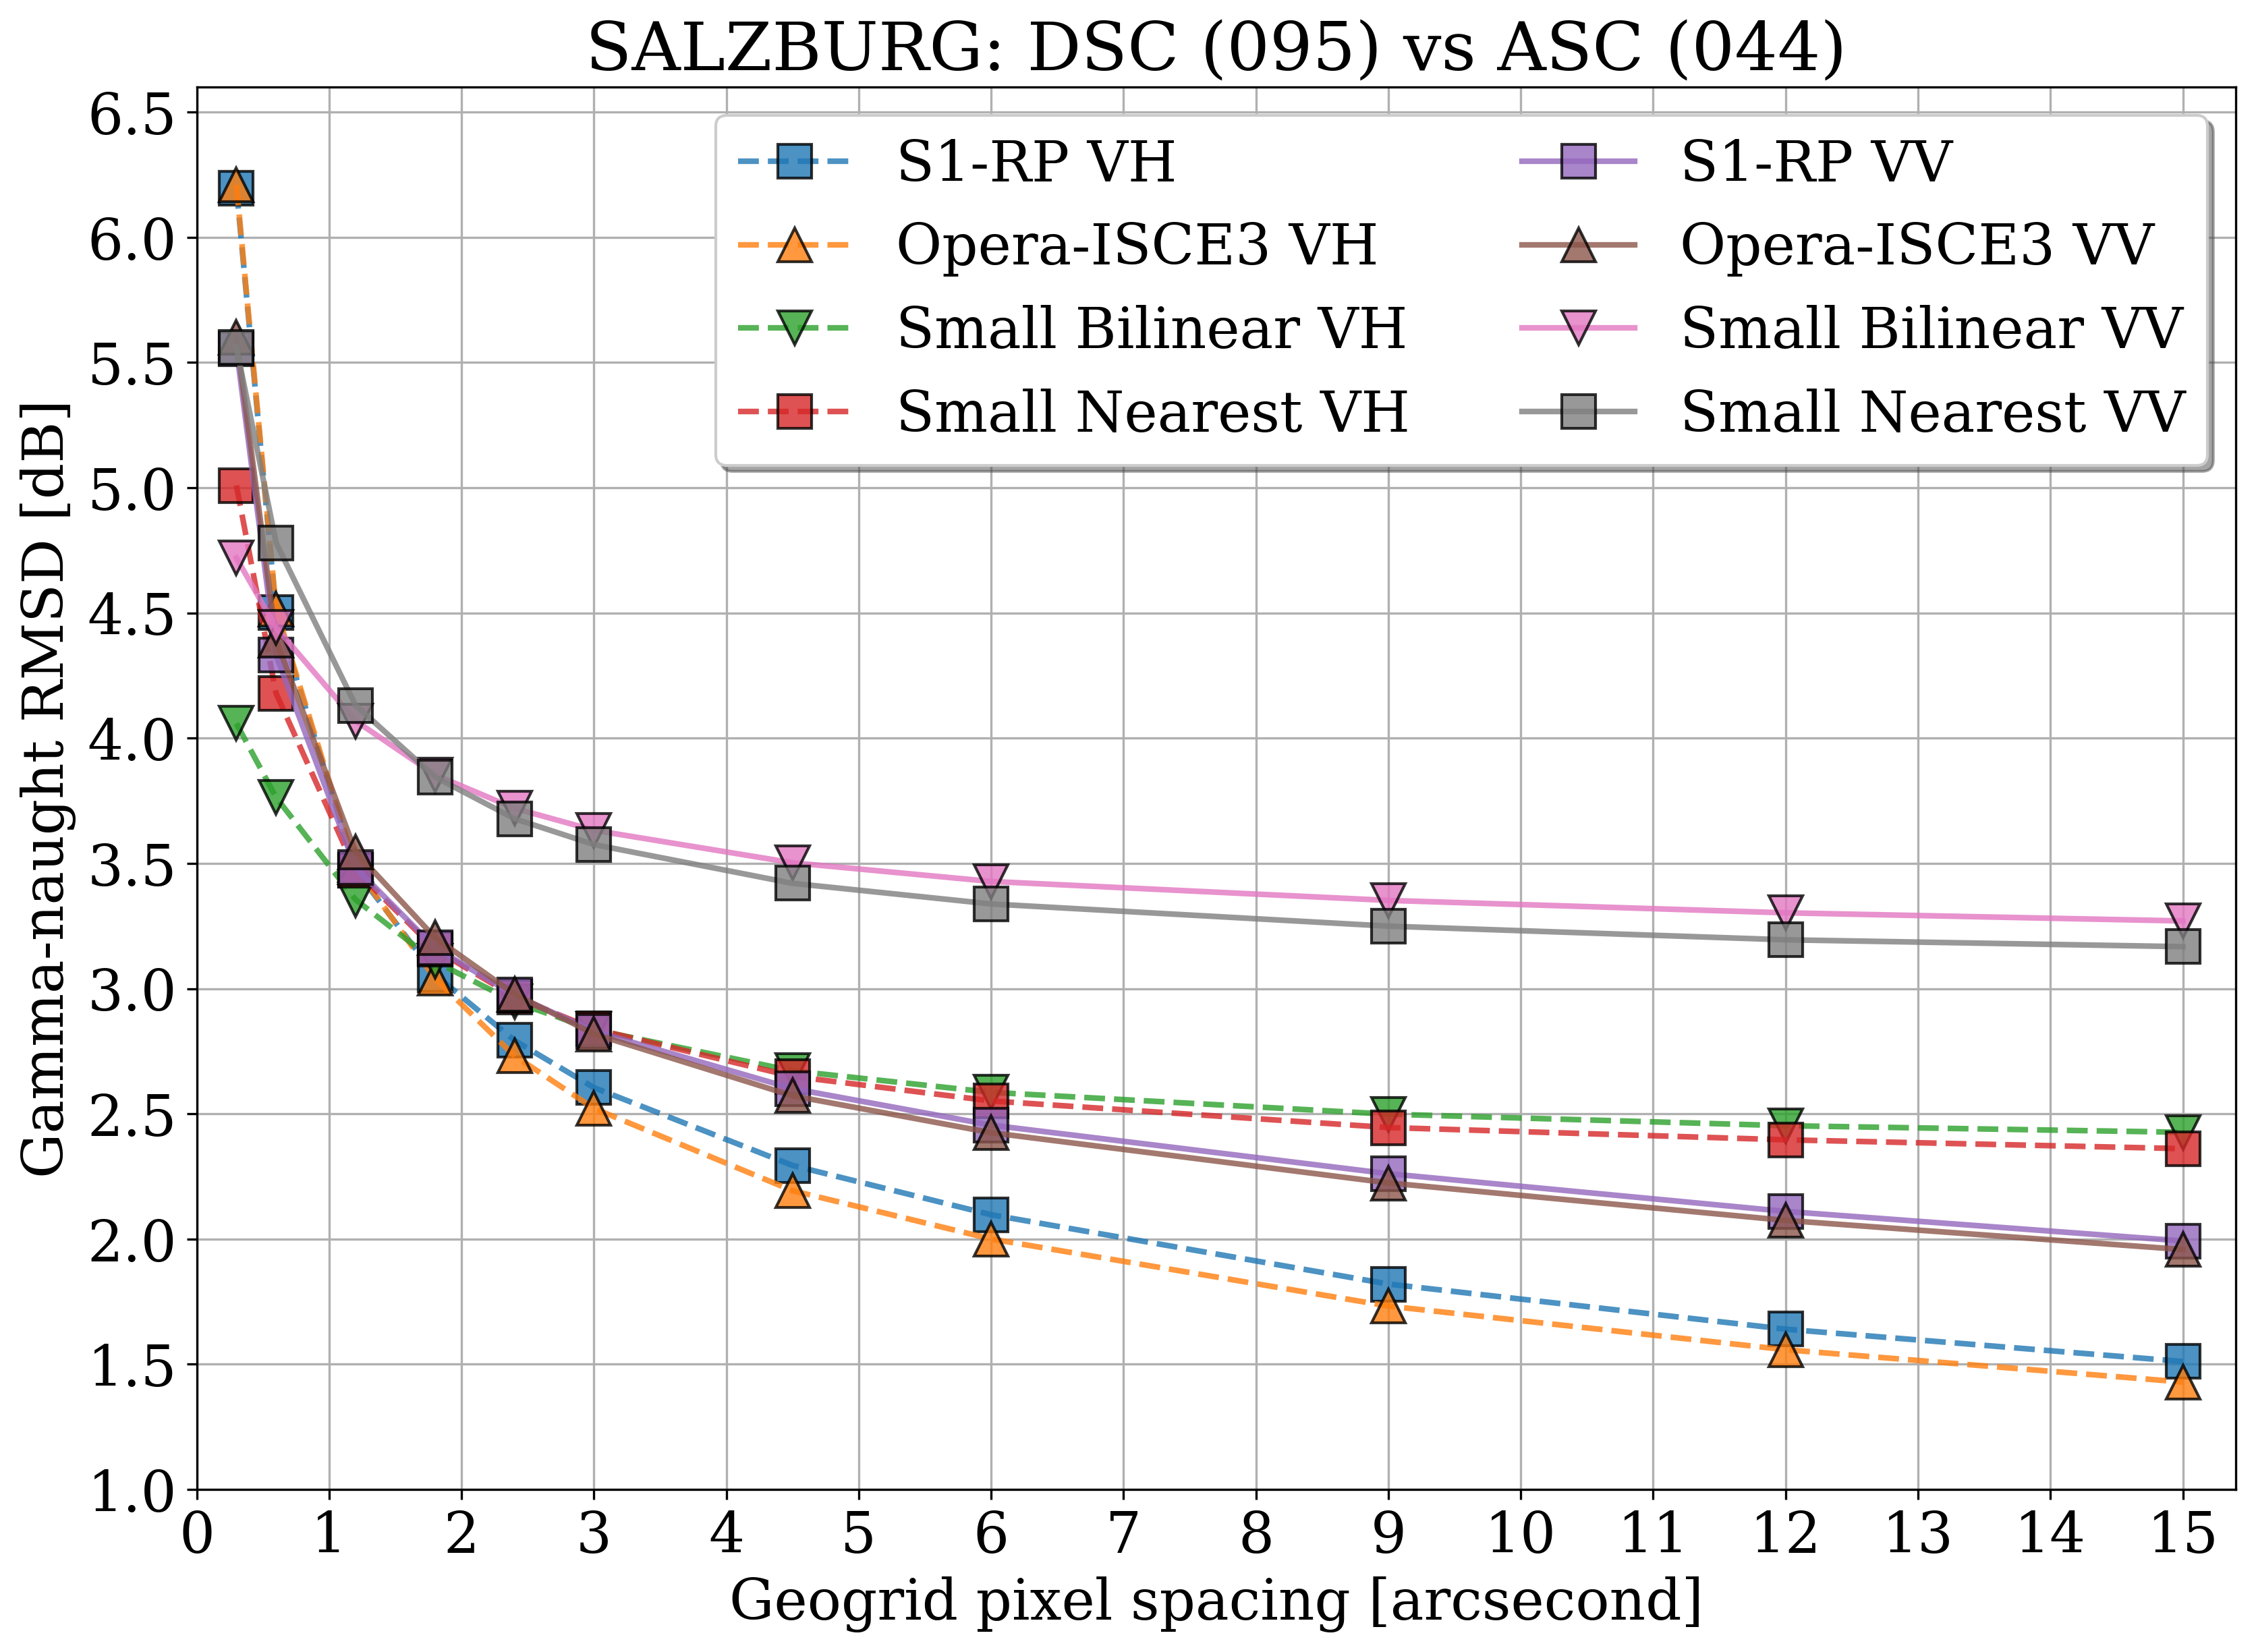
\includegraphics[width=0.9\textwidth]{Figures/nrb/new_salzburg.png}
    \caption{Root mean square difference between ascending and descending NRB products
over Salzburg, using COPDEM10m and multilooked resolutions from $0.3$ arcseconds up to $15$ arcseconds.}
    \label{fig:nrbs_comparison}
  \end{figure}

Figure~\ref{fig:nlooks_comparison} shows the histogram of the number of looks on the same area using \acs{s1rp}, OPERA-ISCE3 and the Small C-Code.

\begin{figure}[h!]
  \centering
    \centering
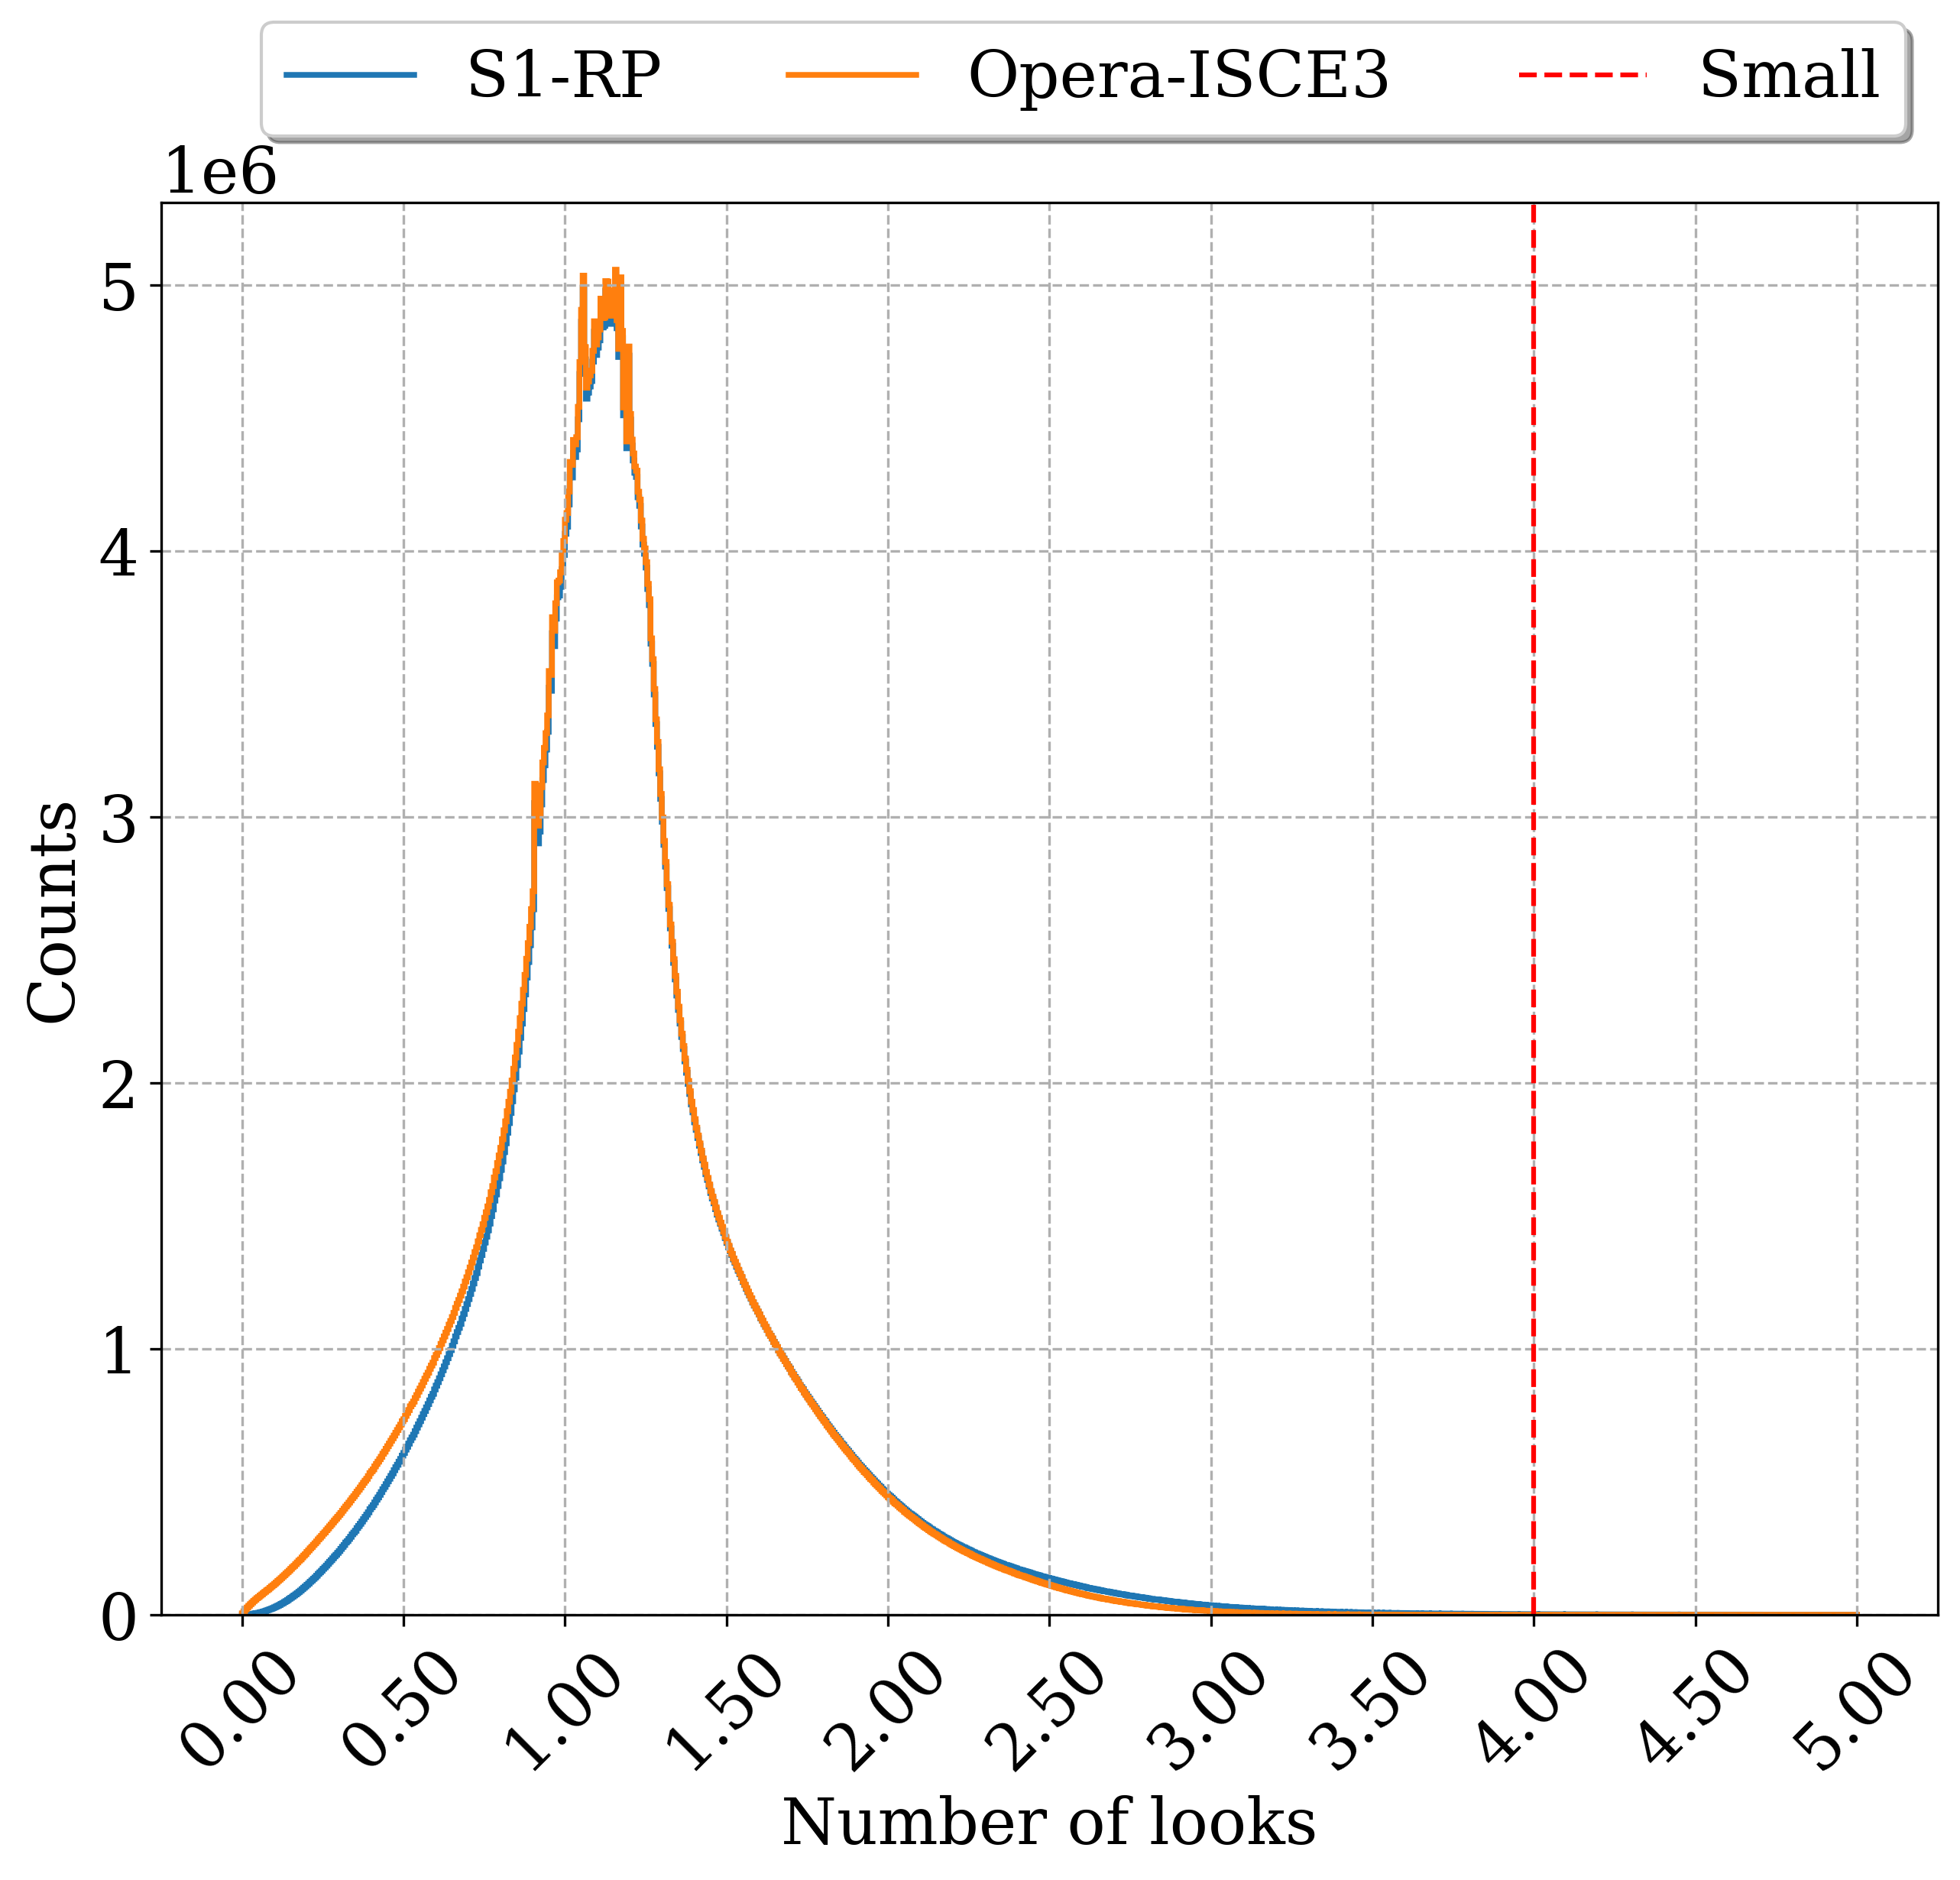
\includegraphics[width=0.7\textwidth]{Figures/nrb/nlooks_salzburg.png}
    \caption{Number of looks comparison on the same area between \acs{s1rp}, Opera-ISCE3 and Small C-Code.}
    \label{fig:nlooks_comparison}
  \end{figure}

As shown in Figure~\ref{fig:nlooks_comparison}, OPERA-ISCE3 and B-Open \acs{s1rp} produce perfectly aligned NRB products, with coincident RMSD values across all different output product spacing. In these area-based implementations, the effective multilook factor is dictated by the ground resolution and the radar to ground mapping geometry. In this example, at $0.3$ arcseconds ground sampling, the look count is approximately $1.12$ over flat terrain and increases with slope (which lowers speckle). Thus, at native resolution, speckle dominates the differences; as the effective number of looks grows (either by coarser sampling or explicit multilooking) the RMSD falls, and no systematic bias remains.

By contrast, the point-based C-Code inherently averages over a larger number of looks even at $0.3$ arcseconds resolution, yielding lower RMSD than the area-based tools (specifically, a constant multilook along both directions is performed, so that the aspect ratio is "squarish": in this example, a constant multilook of 4 along slant range, and a multilook of 1 along azimuth, have been performed). Furthermore, the bilinear interpolation step (recommended option) further increases the number of looks, and this is evident by comparing this approach with the Nearest Neighbor's one, as shown in Figure~\ref{fig:nrbs_comparison}.

However, when the output is coarsened by spatial averaging, the point-based algorithm still exhibits a residual bias of about 1 dB relative to the area-based algorithm. This remaining offset could reflects the different compensation model employed by the point-based approach.

\subsubsection{Stability of radiometric response over varying acquisition conditions}
\label{sec:nrb_stability_diff_geom}
The generation of \acs{nrb} products involves two main steps:

\begin{itemize}
    \item \textbf{\acs{anf} correction (gamma flattening)}: this step removes the dependency of the radar cross-section on the local terrain slope by applying a multiplicative compensation factor derived from a digital elevation model (DEM). It counteracts the radiometric distortions caused by foreshortening and shadowing.  
    \item \textbf{Geocoding}: this transforms data from radar geometry (slant range and azimuth) into ground coordinates (e.g.\ latitude, longitude) using the same projection matrix computed during the slope compensation stage.  
\end{itemize}

Figure~\ref{fig:Salzburg_044_VV_nocorr} shows a geocoded mosaicked NRB image over Salzburg without applying the \acs{anf} correction. Although the data are correctly projected, pixels located in foreshortened or layover zones appear artificially bright, while those in shadowed areas are unnaturally dark. After applying gamma flattening, as seen in Figure~\ref{fig:Salzburg_044_VV_corr}, these slope-induced radiometric artifacts are effectively removed, yielding a more uniform backscatter response across varying topography.

\begin{figure}[htbp]
  \centering
  \begin{subfigure}[b]{0.48\textwidth}
    \centering
    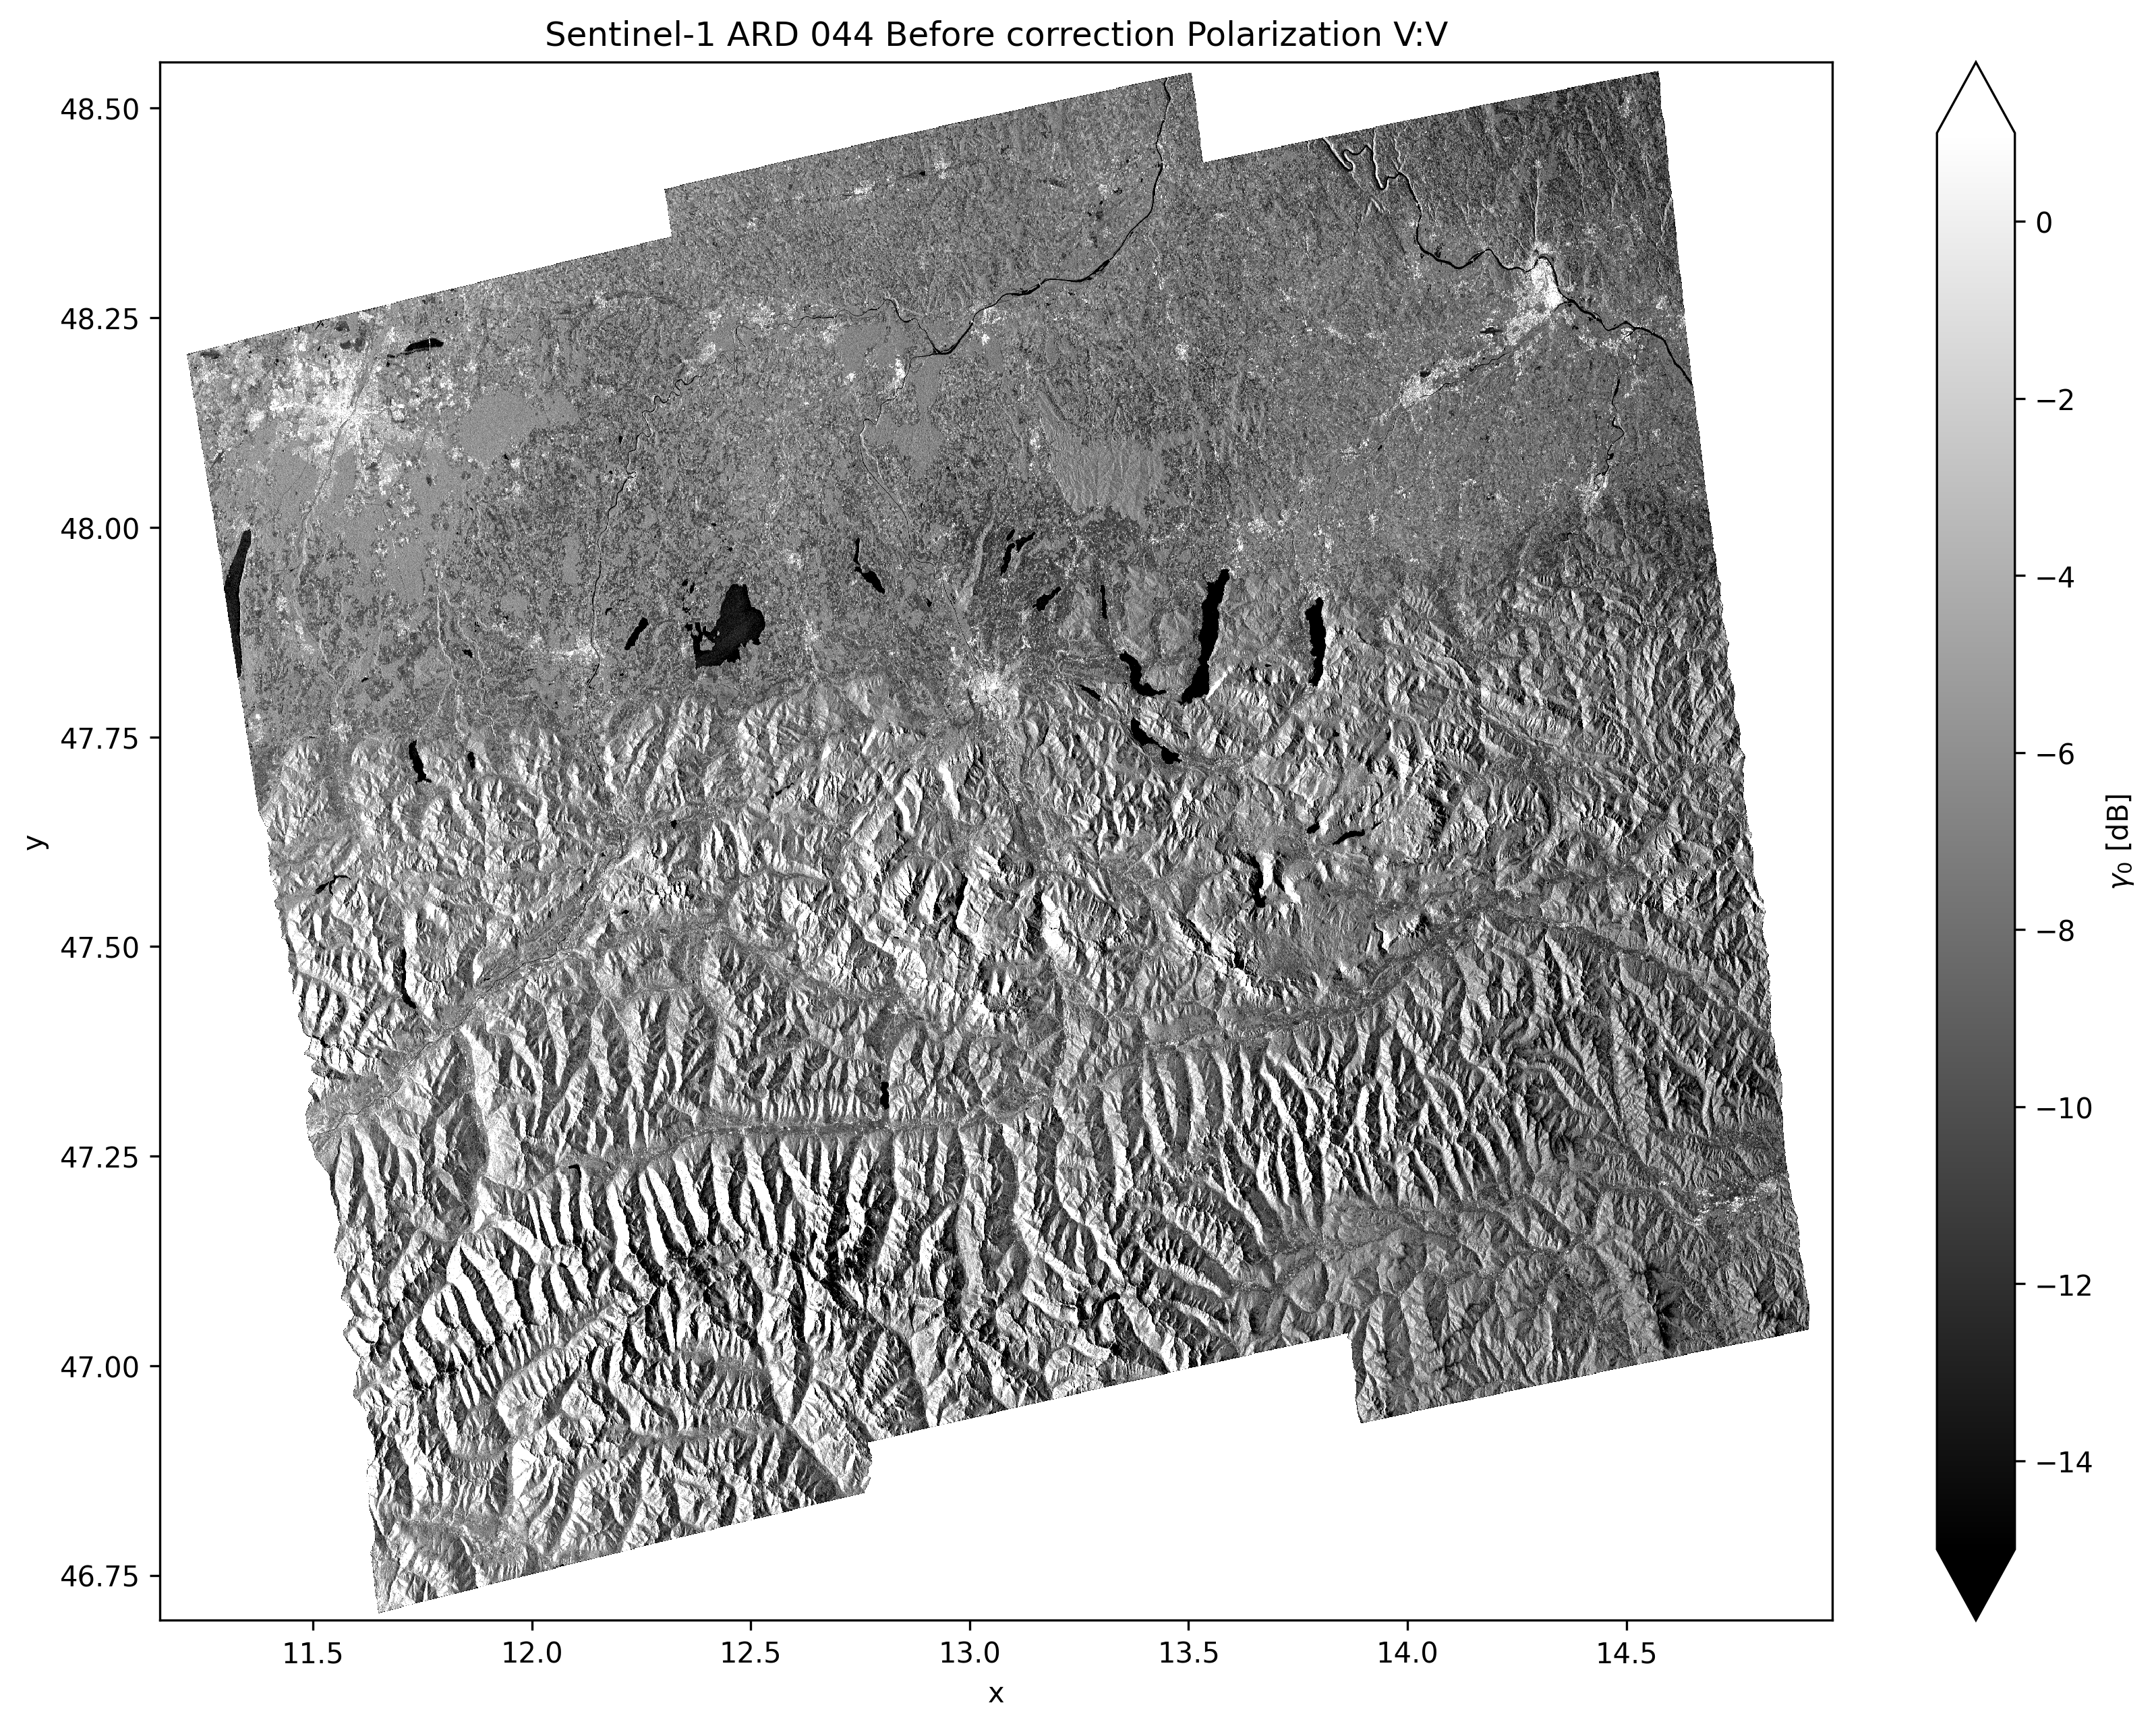
\includegraphics[width=\textwidth]{Figures/nrb/Salzburg_044_VV_nocorr.png}
    \caption{Without \acs{anf} correction}
    \label{fig:Salzburg_044_VV_nocorr}
  \end{subfigure}
  \hfill
  \begin{subfigure}[b]{0.48\textwidth}
    \centering
    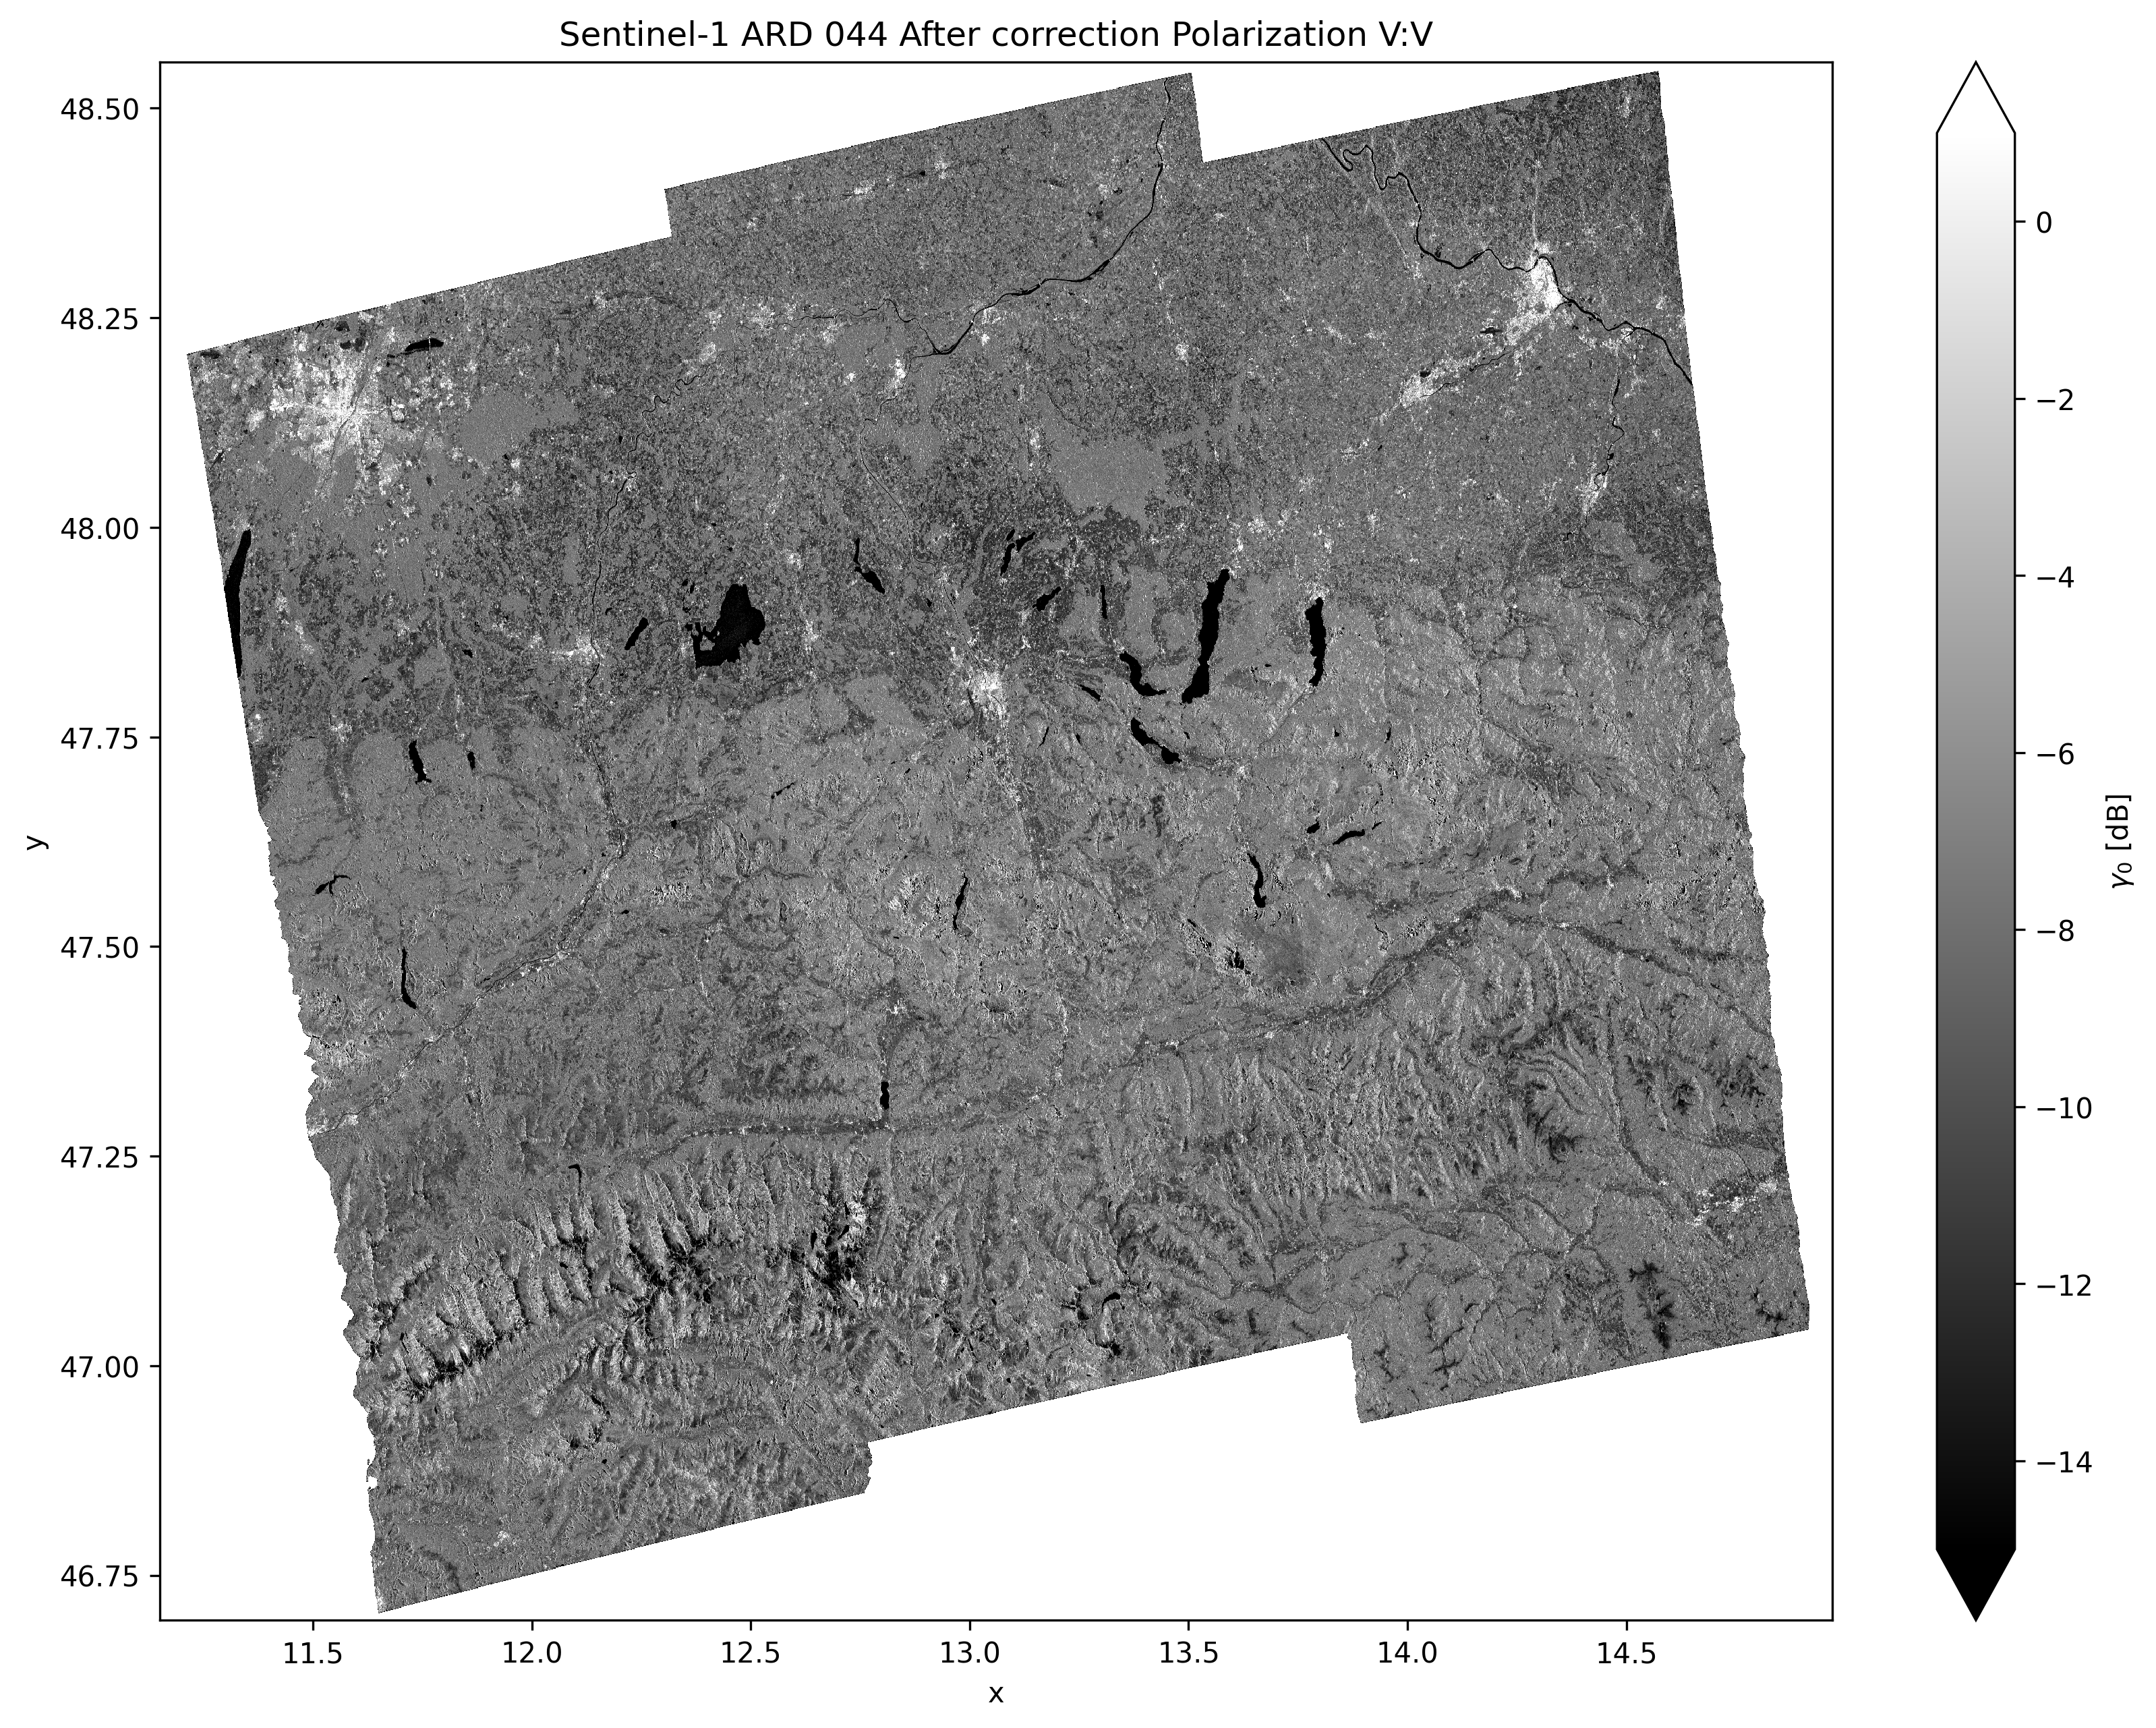
\includegraphics[width=\textwidth]{Figures/nrb/Salzburg_044_VV_corr.png}
    \caption{With \acs{anf} correction}
    \label{fig:Salzburg_044_VV_corr}
  \end{subfigure}
  \caption{Mosaicked NRB images of Salzburg before (left) and after (right) terrain slope flattening.}
  \label{fig:due_subfigure}
\end{figure}
This visual inspection provides qualitative insight only. To quantify the effectiveness of slope removal, we designed two tests:

\begin{itemize}
    \item \textit{Correlation index between NRB and terrain slope}  
    \item \textit{Slope compensation consistency across acquisition geometries}
\end{itemize}

\paragraph{Correlation index between NRB and terrain slope}

We processed a Sentinel-1 dataset over a steep alpine region twice: once including the slope compensation stage and once omitting it. For each version, we derived the local slope angle from a high-resolution DEM and constructed two-dimensional histograms of NRB values versus slope angle. This approach highlights any residual coupling between backscatter intensity and topography.

Figure~\ref{fig:hist_2d_no_corr} presents the histogram without compensation, where a clear diagonal band indicates that steeper terrain systematically biases the backscatter—higher incidence angles yield consistently different NRB values. Figure~\ref{fig:hist_2d_corr} shows the histogram after flattening: the diagonal structure nearly vanishes and NRB values distribute uniformly across all slopes, demonstrating effective removal of topographic dependency.

\begin{figure}[htbp]
  \centering
  \begin{subfigure}[b]{0.48\textwidth}
    \centering
    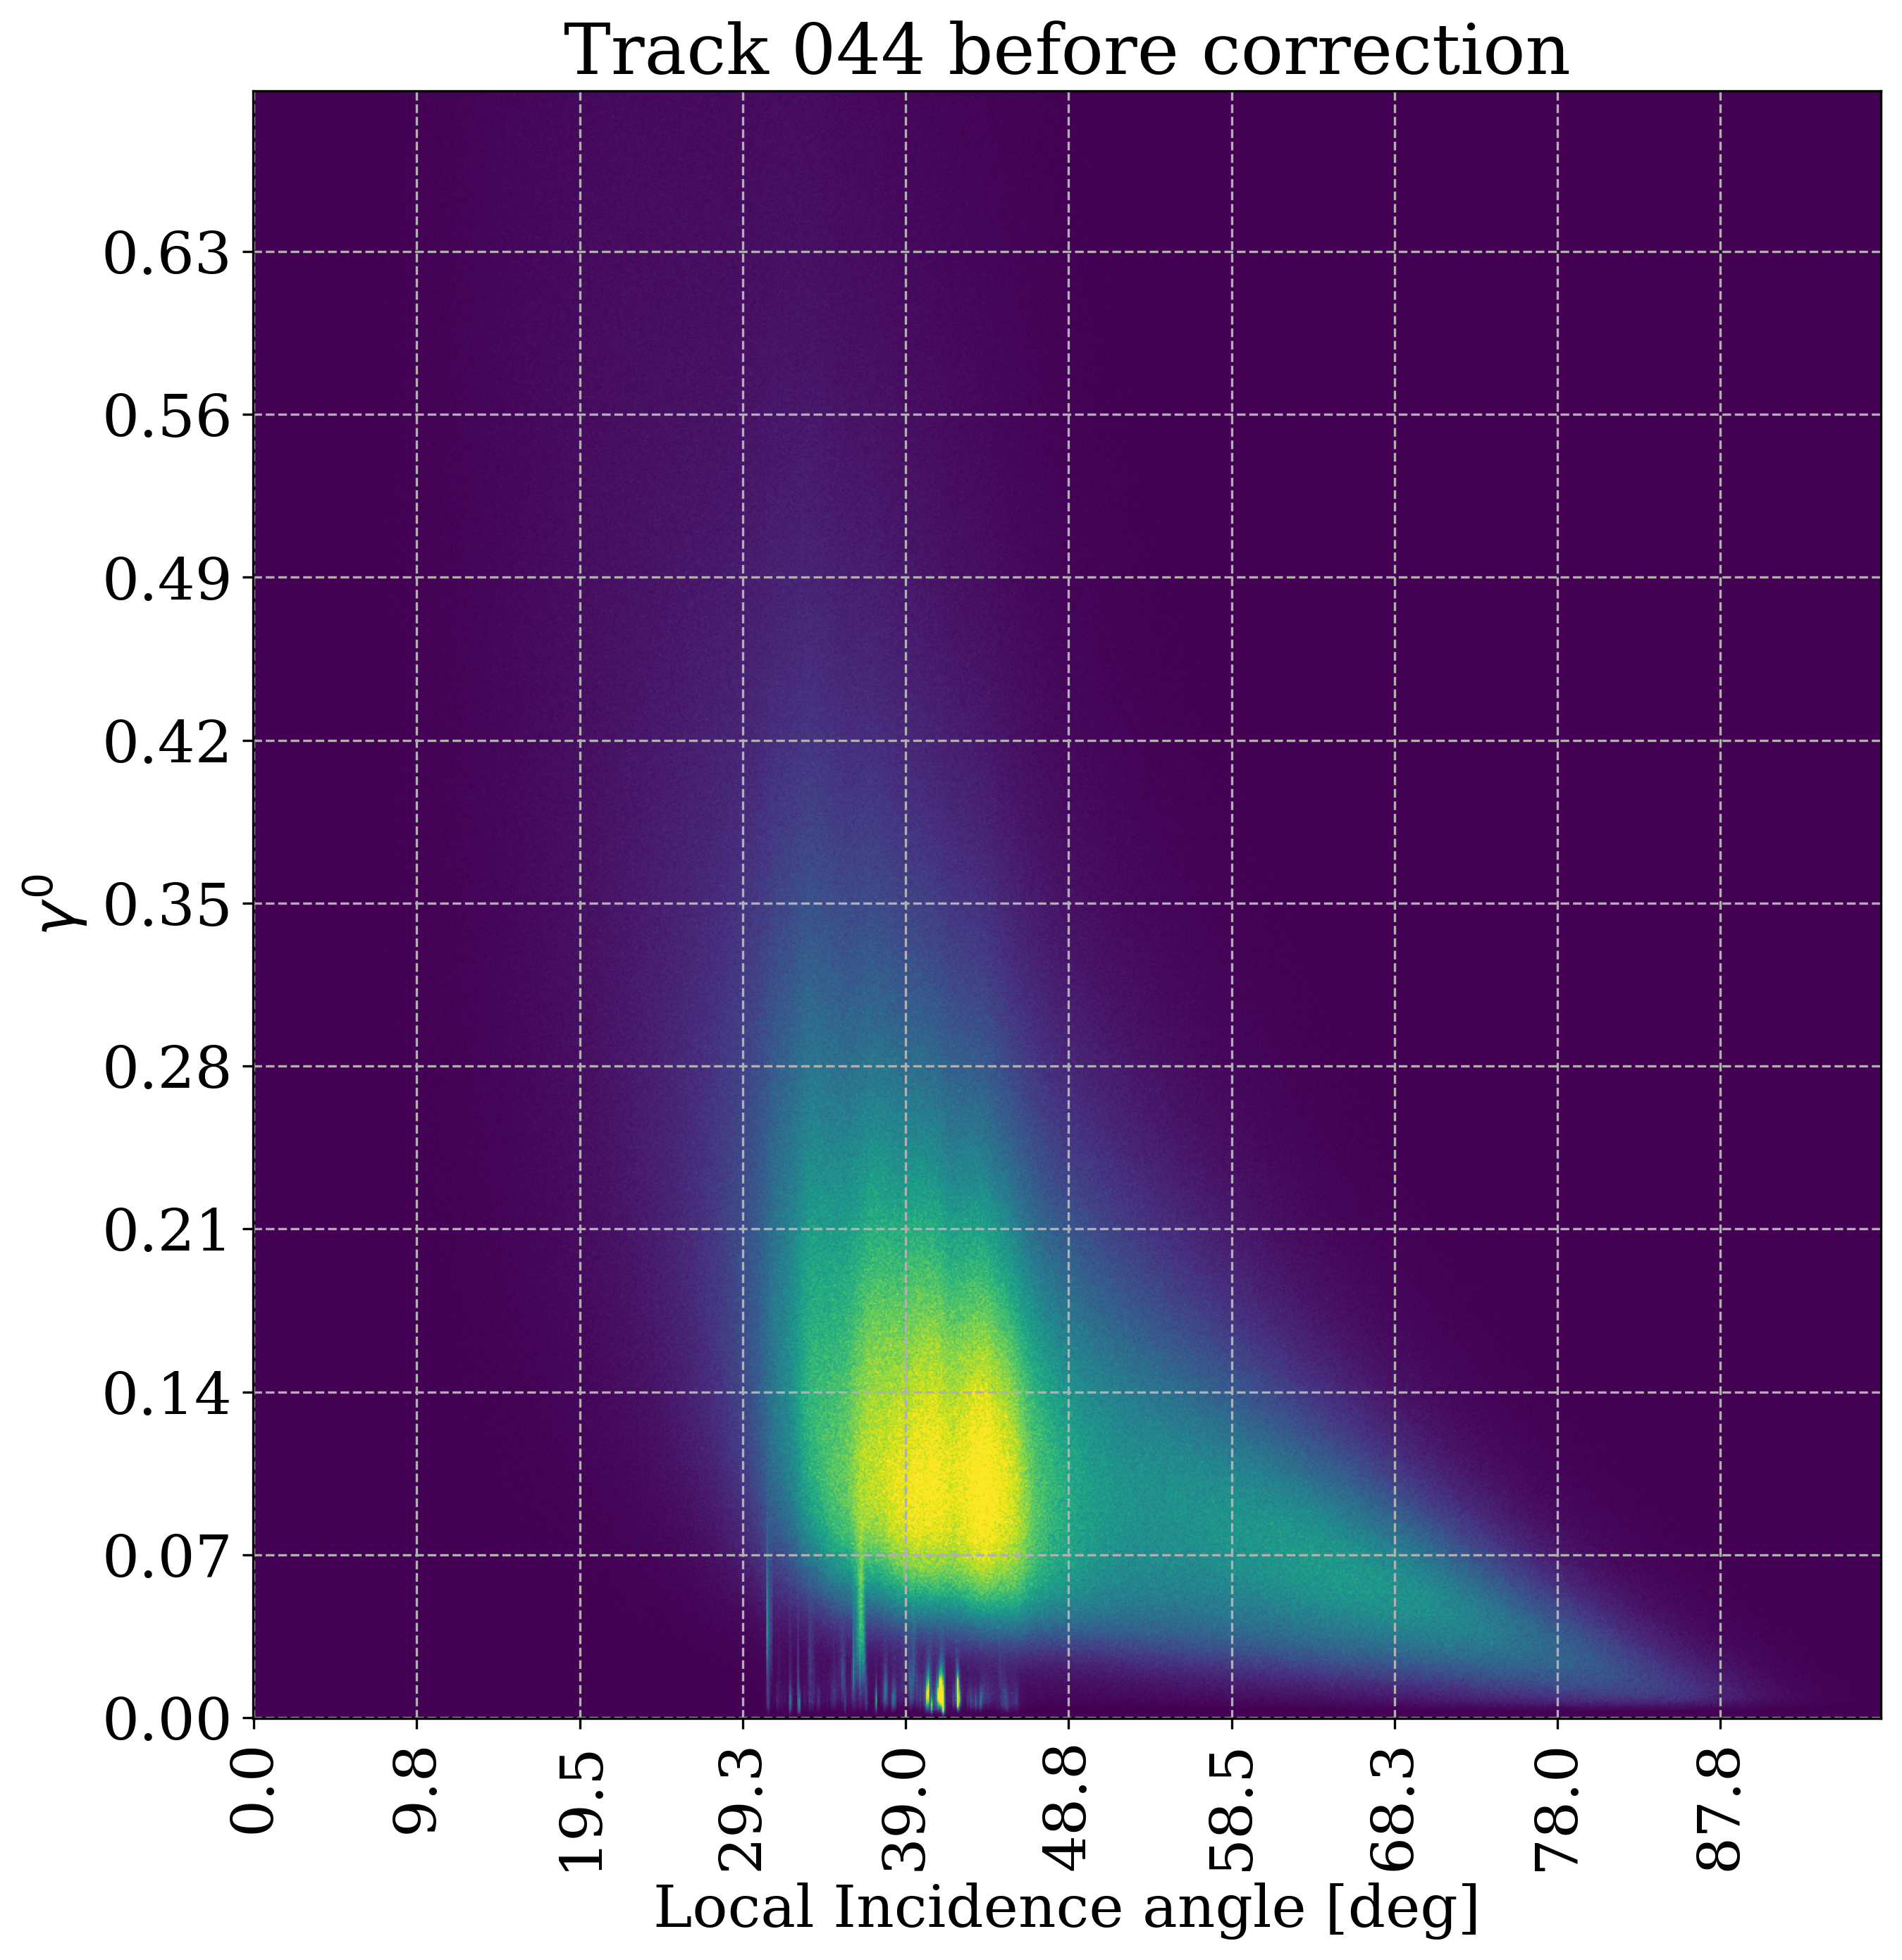
\includegraphics[width=\textwidth]{Figures/nrb/hist_2d_no_corr.png}
    \caption{}
    \label{fig:hist_2d_no_corr}
  \end{subfigure}
  \hfill
  \begin{subfigure}[b]{0.48\textwidth}
    \centering
    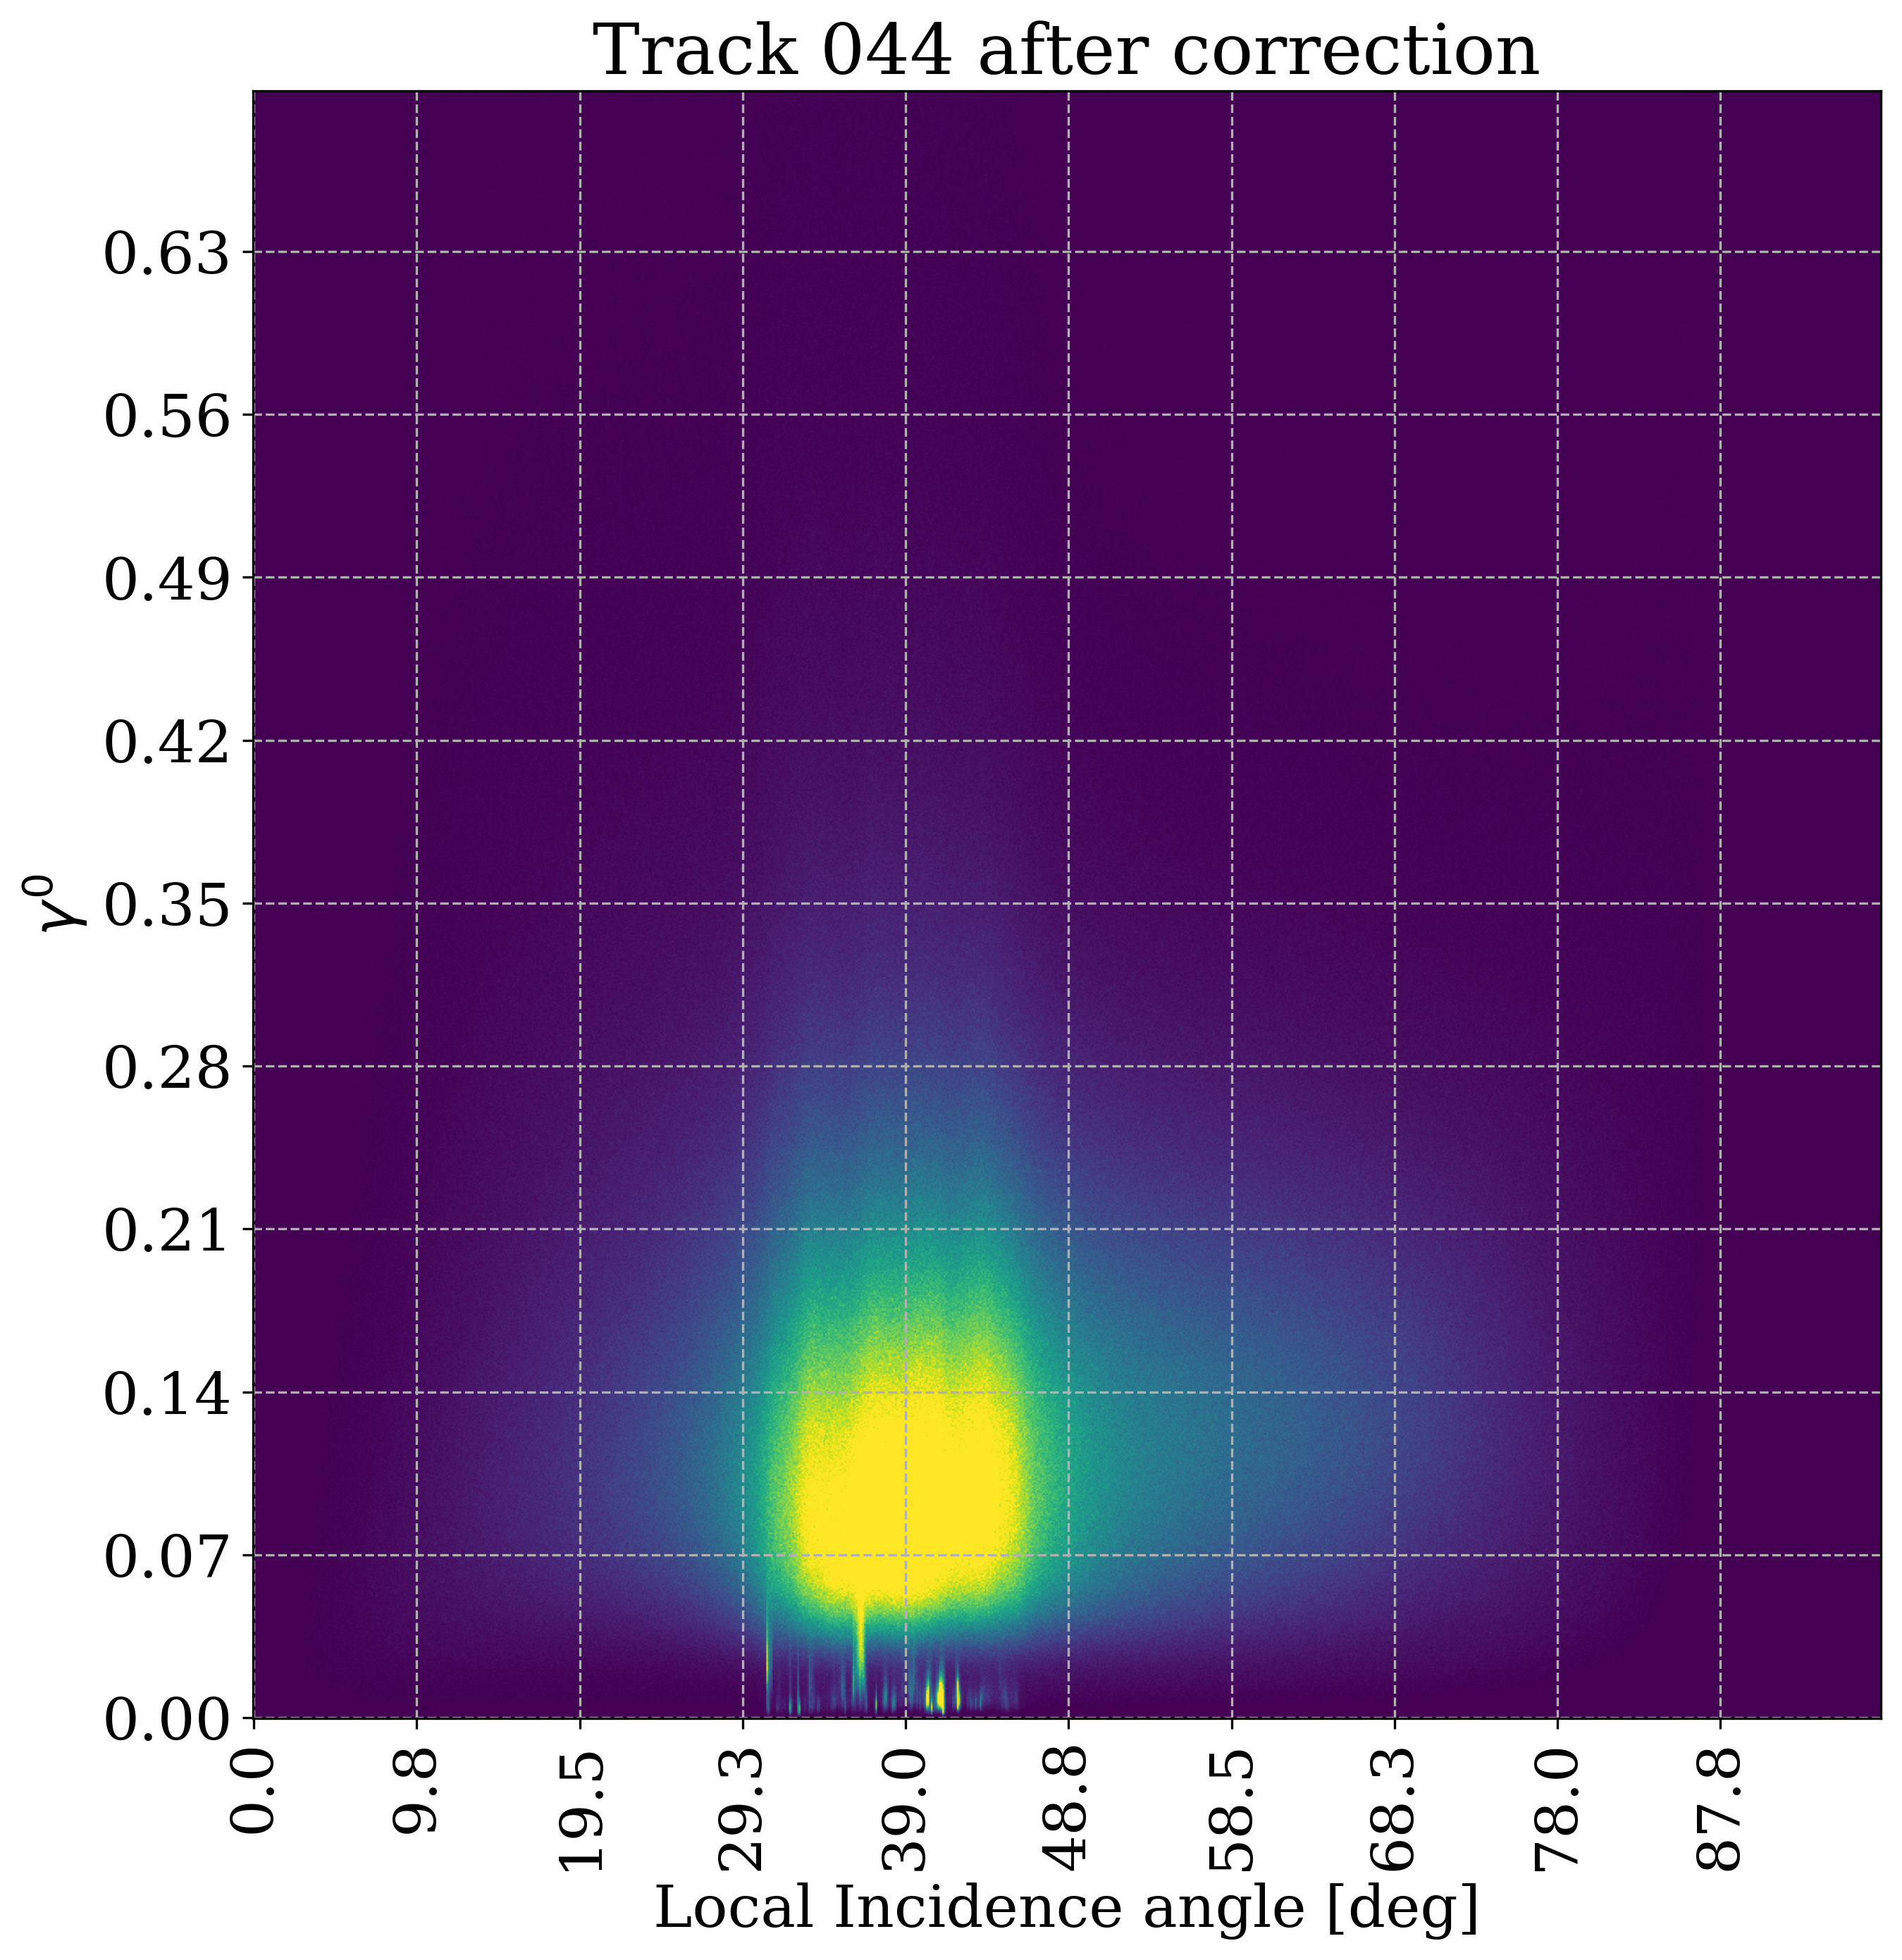
\includegraphics[width=\textwidth]{Figures/nrb/hist_2d_corr.png}
    \caption{}
    \label{fig:hist_2d_corr}
  \end{subfigure}
  \caption{Two-dimensional histograms of NRB versus local slope angle before (a) and after (b) applying the \acs{anf} correction.}
  \label{fig:due_subfigure}
\end{figure}

To further quantify this improvement, we divided the study area into non overlapping patches of size $1000\times1000$ pixels and computed the Pearson correlation coefficient between mean NRB and mean slope angle in each patch. Figure~\ref{fig:correlation_salzburg} plots these coefficients for Sentinel-1 tracks 044 (ascending) and 095 (descending) over Salzburg. Yellow squares correspond to uncorrected data, with correlation values mostly between 0.1 and 0.5. Red circles show the flattened products, where nearly all correlations cluster around zero—confirming the slope compensation step’s ability to eliminate topographically induced radiometric bias.

\begin{figure}[h!]
  \centering
  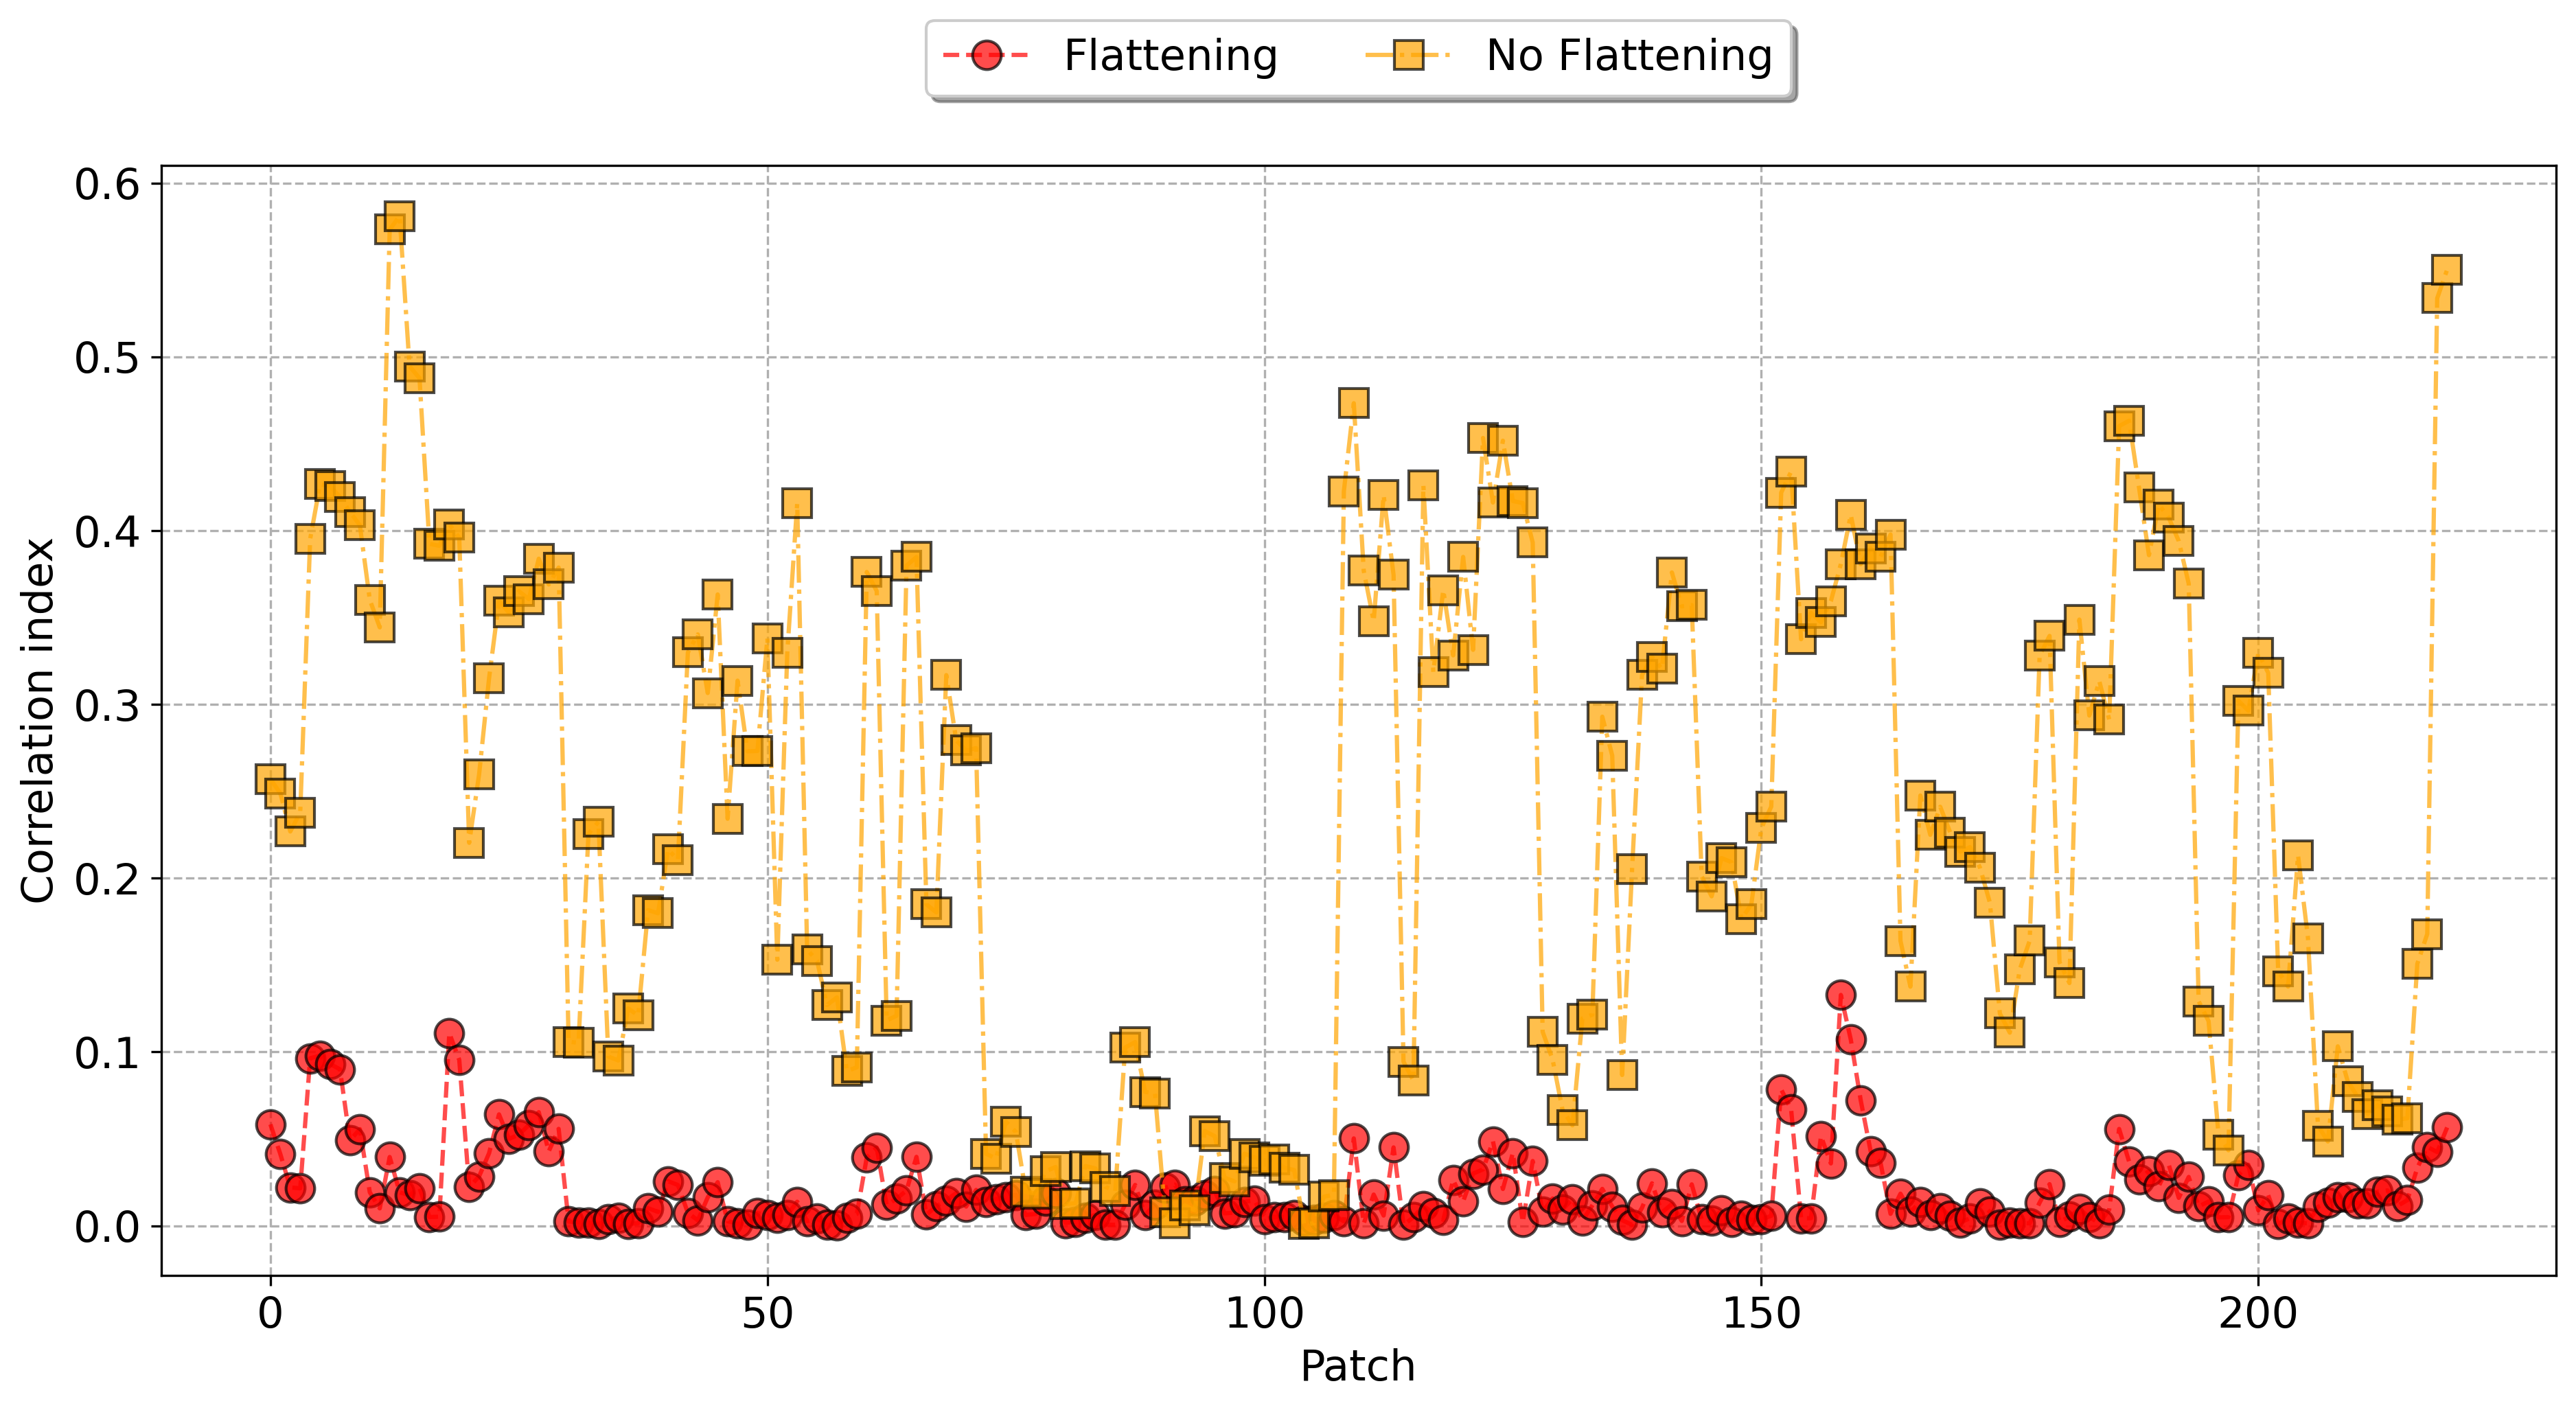
\includegraphics[width=0.9\textwidth]{Figures/nrb/correlation_salzburg.png}
  \caption{Pearson correlation between mean NRB and mean slope angle across $1000\times1000$ pixel patches, before (yellow) and after (red) \acs{anf} correction. Data derive from Sentinel-1 tracks 044 and 095 over Salzburg.}
  \label{fig:correlation_salzburg}
\end{figure}

\paragraph{Slope compensation consistency across acquisition geometries}

We assessed consistency by computing the root mean square difference (RMSD) between ascending and descending acquisitions over identical terrain, as shown in Figure~\ref{fig:rmsd_salzburg}. The analysis used the B-Open S1-RP software on Sentinel-1 IW datasets (tracks 044 and 095) over Salzburg, Austria. Products were first generated at a native 10 m ground resolution; subsequent coarser resolutions (up to 500 m) were obtained via multilooking as described in Section~\ref{sec:nrb_multilook}. 

At the native 10 m resolution, RMSD values range from 3.7 dB to 5.5 dB, dominated by speckle. After multilooking to 500 m, the effect of speckle diminishes markedly, yielding RMSD of about 1.2 dB for the 10 m DEM geogrid and 1.7 dB for the 30 m DEM geogrid. These findings confirm that slope flattening, eventually combined with appropriate multilooking, delivers robust NRB products independent of viewing geometry.

\begin{figure}[h!]
  \centering
  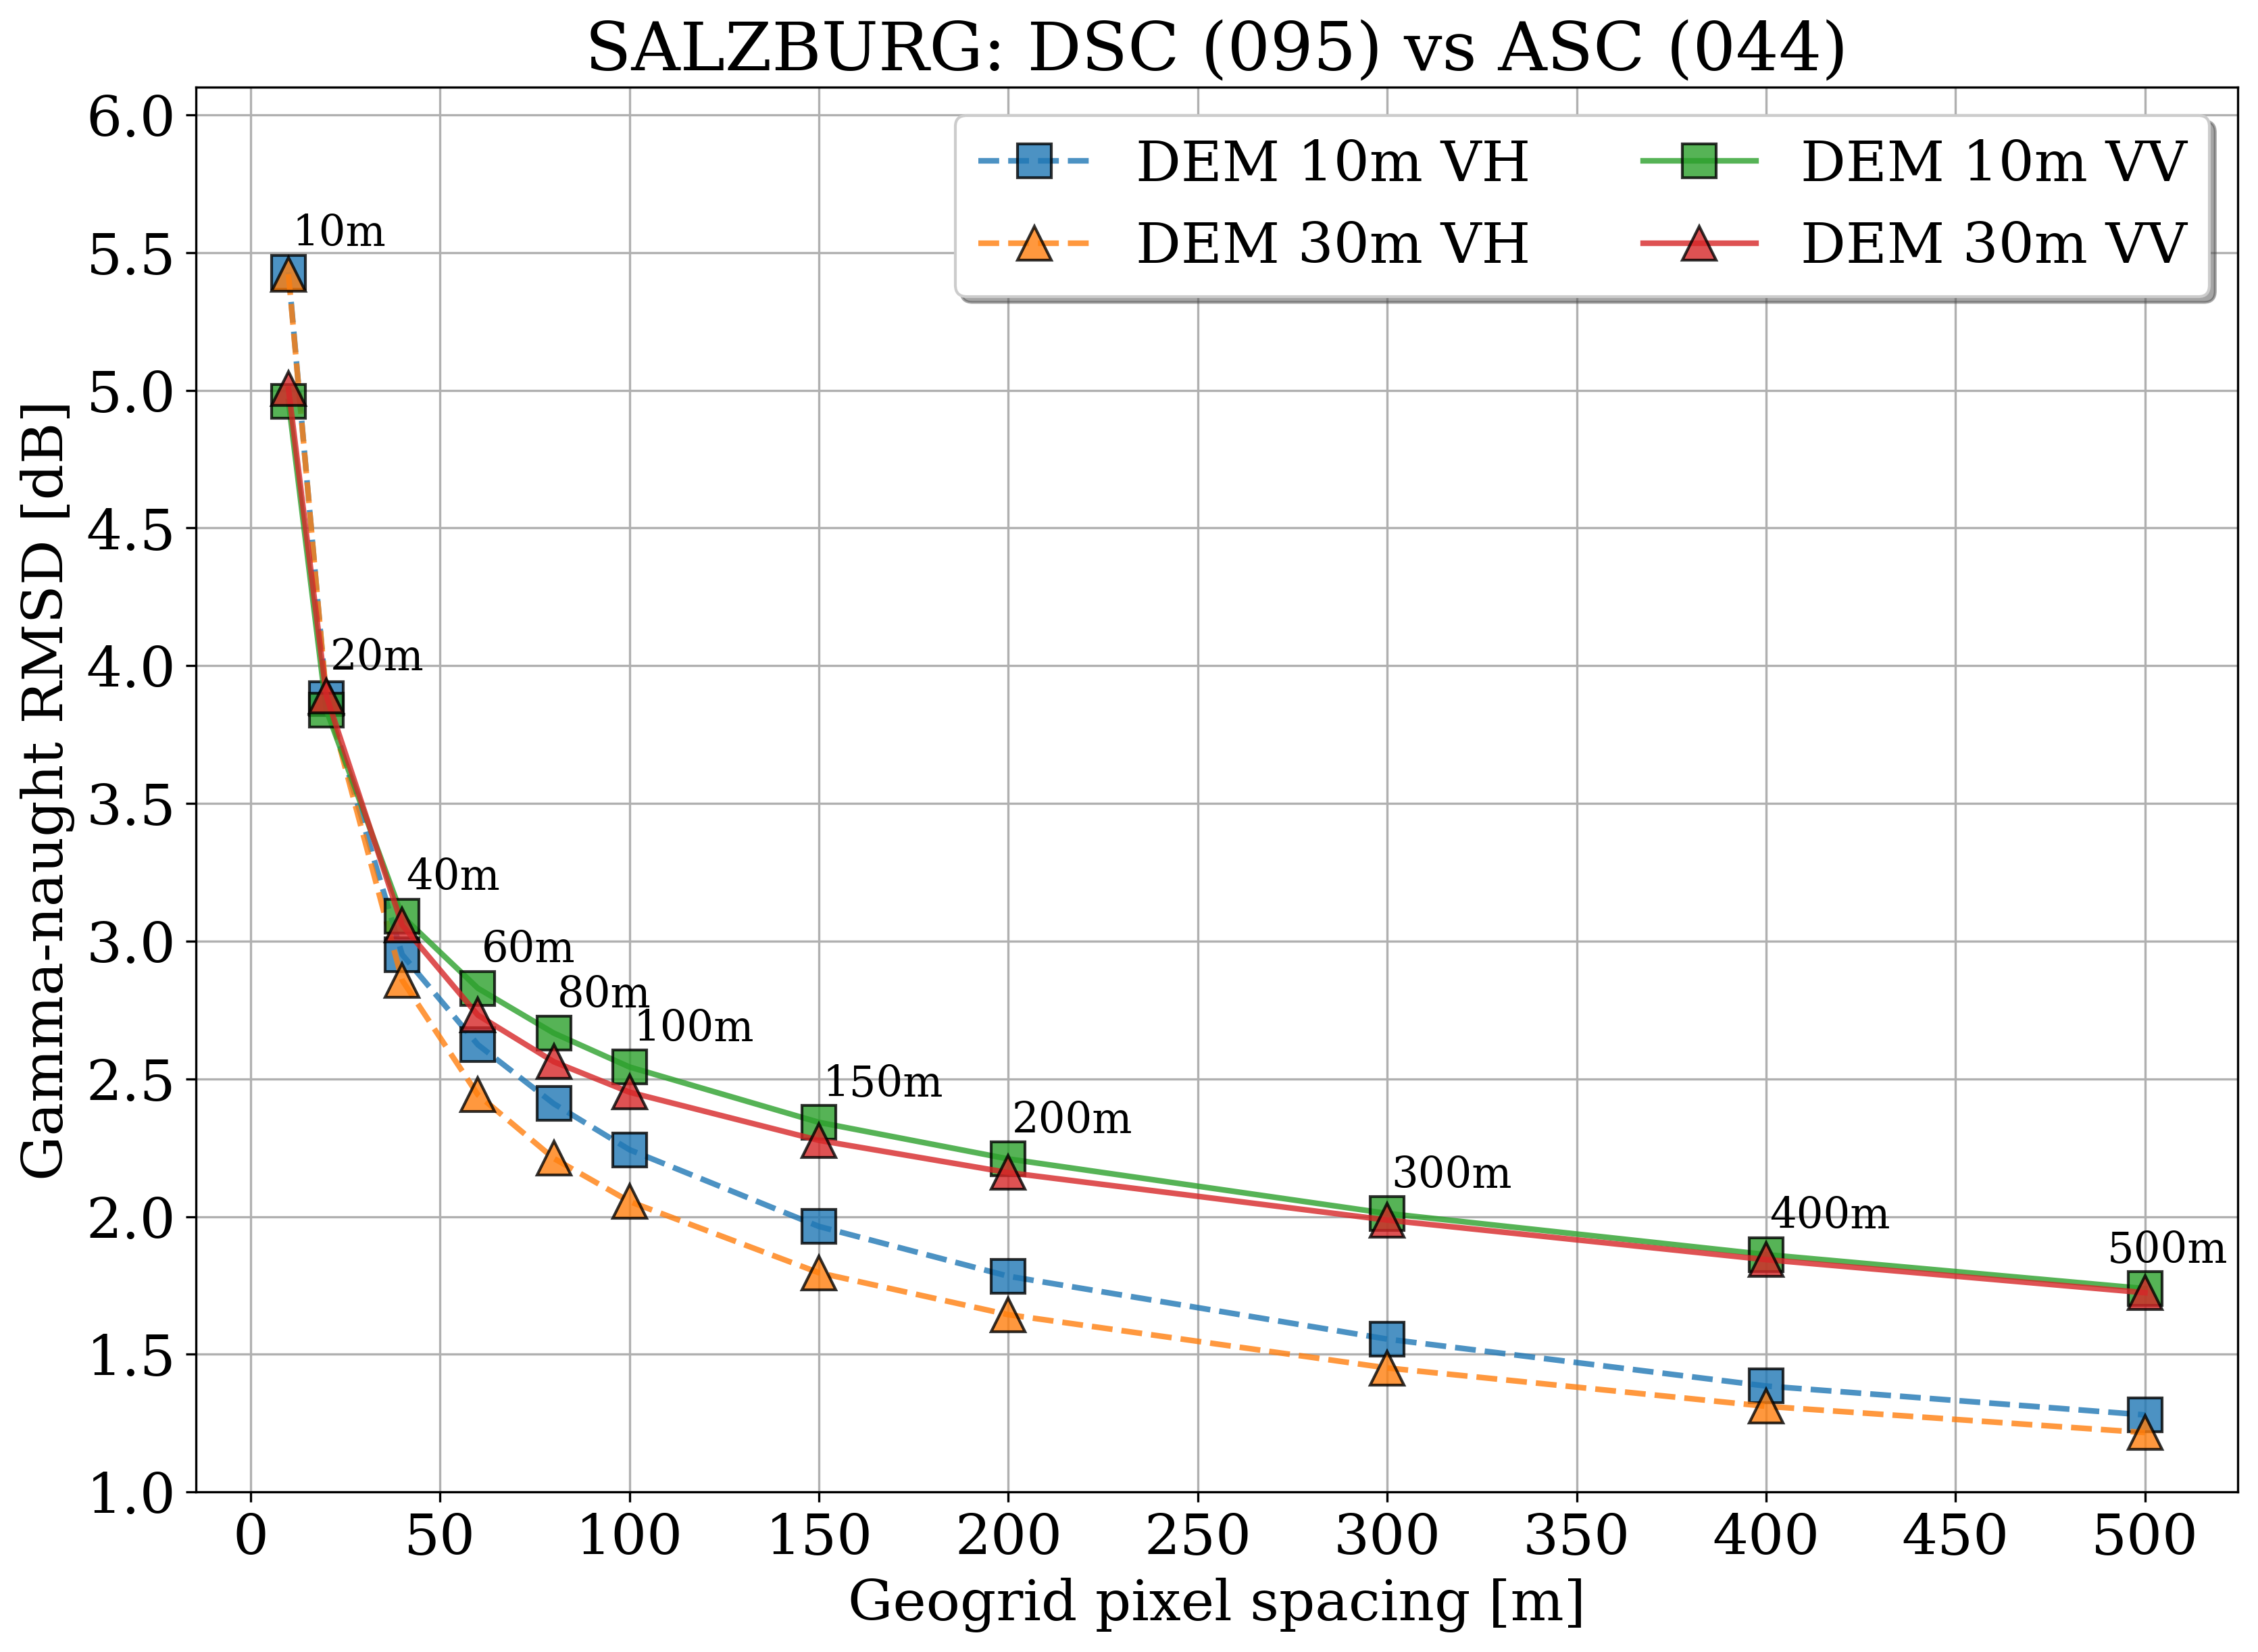
\includegraphics[width=0.9\textwidth]{Figures/nrb/db_with_10m.png}
  \caption{Root mean square difference between ascending and descending NRB products over Salzburg, using DEM geogrids of 10 m and 30 m and multilooked resolutions from 10 m up to 500 m.}
  \label{fig:rmsd_salzburg}
\end{figure}

\subsection{Dependence on External Data}
\label{sec:nrb_dependence_external}

\subsubsection{Dependence on DEM Resolution and Quality}

The accuracy of radiometric terrain correction in complex terrain relies critically on the resolution and vertical accuracy of the Digital Elevation Model (DEM). A high resolution DEM captures local slope variations and terrain morphology more precisely, enabling more accurate estimation of the local incidence angle and illuminated ground area. Conversely, coarser or error-prone DEMs smooth out fine scale slopes and introduce biases in the computed Area Normalization Factor (ANF), which in turn degrade the quality of the generated NRB product.

\paragraph{Theoretical model}
\label{sec:nrb_theoretical_model_dem}

For a single DEM facet the ANF is defined as the projection of a slant range pixel’s ground footprint onto a plane orthogonal to the sensor’s line of sight. Let \(A\) be the true ground cell area and \(\theta_i\) the local incidence angle (the angle between the radar line of sight and the normal to the DEM facet). Then
\begin{equation}
  \label{eq:ANF}
  \gamma_{\mathrm{ANF}} \;=\; A \,\cos\!\theta_i.
\end{equation}

Considering that multiple DEM facets can partially contribute to the same radar cell, let \(j\) be the index of the DEM facet, let \(l\) be the index of the radar cell, let \(J(l)\) the set of DEM facets covering the radar cell \(l\), let \(w_{j,l}\) the percentage of coverage of the radar cell \(l\) by the DEM facet \(j\), the ANF associate to the radar cell is given by:

\begin{equation}
  \label{eq:ANF_integral}
  \gamma_{\mathrm{ANF}_l} = \sum_{j \in J(l)} A_j w_{j,l} \cos\!\theta_{i_j} \,\bigl(1 - \delta\theta_{i_j} \tan\!\theta_{i_j}\bigr).
\end{equation}

In order to simplify the equation and evaluate the error on the ANF it is possible to identify an upper-bound for the local incidence angle and the value of \(\delta\theta\).

If the DEM has an elevation error \(\sigma_h\), this propagates into an incidence angle error \(\delta\theta_i\approx \sigma_h / dx\), where \(dx\) is the horizontal DEM sampling. A first order Taylor expansion of \eqref{eq:ANF} yields
\begin{equation}
  \label{eq:ANF_first_ord}
  |\Delta \gamma_{\mathrm{ANF}_l}| \le \sum_{j \in J(l)} A_j w_{j,l} \cos\!\theta_{i_j} \,\bigl(\delta\theta_{\mathrm{max}} \tan\!\theta_{\mathrm{max}}\bigr) = \gamma_{\mathrm{ANF}_l} \bigl(\delta\theta_{\mathrm{max}} \tan\!\theta_{\mathrm{max}}\bigr).
\end{equation}
Thus, the variance of the ANF error due to DEM noise is
\begin{equation}
  \sigma^2_{\gamma_{\mathrm{ANF}_h}}
  = \gamma^2_{\mathrm{ANF}}
    \Bigl(\tfrac{\tan\!\theta_{\mathrm{max}}}{dx}\Bigr)^{\!2}\,\sigma^2_h.
\end{equation}
This expression shows that DEM errors have the greatest impact where the slope (and hence \(\tan\theta_{\mathrm{max}}\)) is large, and diminish as the DEM pixel size \(dx\) increases.

\paragraph{Test on real data}

To quantify this effect, we computed the ANF over a steep alpine test area using two Copernicus DEMs sampled at \(10\) m and \(30\) m. We then evaluated the ratio in dB between the two ANFs:
\[
  \Delta_{\mathrm{ANF}}(\mathrm{dB})
  = 10\log_{10}\!\bigl(\gamma_{\mathrm{ANF}}^{10\mathrm{m}} / \gamma_{\mathrm{ANF}}^{30\mathrm{m}}\bigr).
\]
Figure~\ref{fig:ANF_DIFF_DB_DEM} maps this difference. As predicted by \eqref{eq:ANF_first_ord}, the largest deviations (up to \(1\)\,dB) occur on the steepest slopes. Smaller but not negligible differences also appear over urban or flat terrain where fine scale surface features are not captured by the coarser DEM.

\begin{figure}[h!]
  \centering
  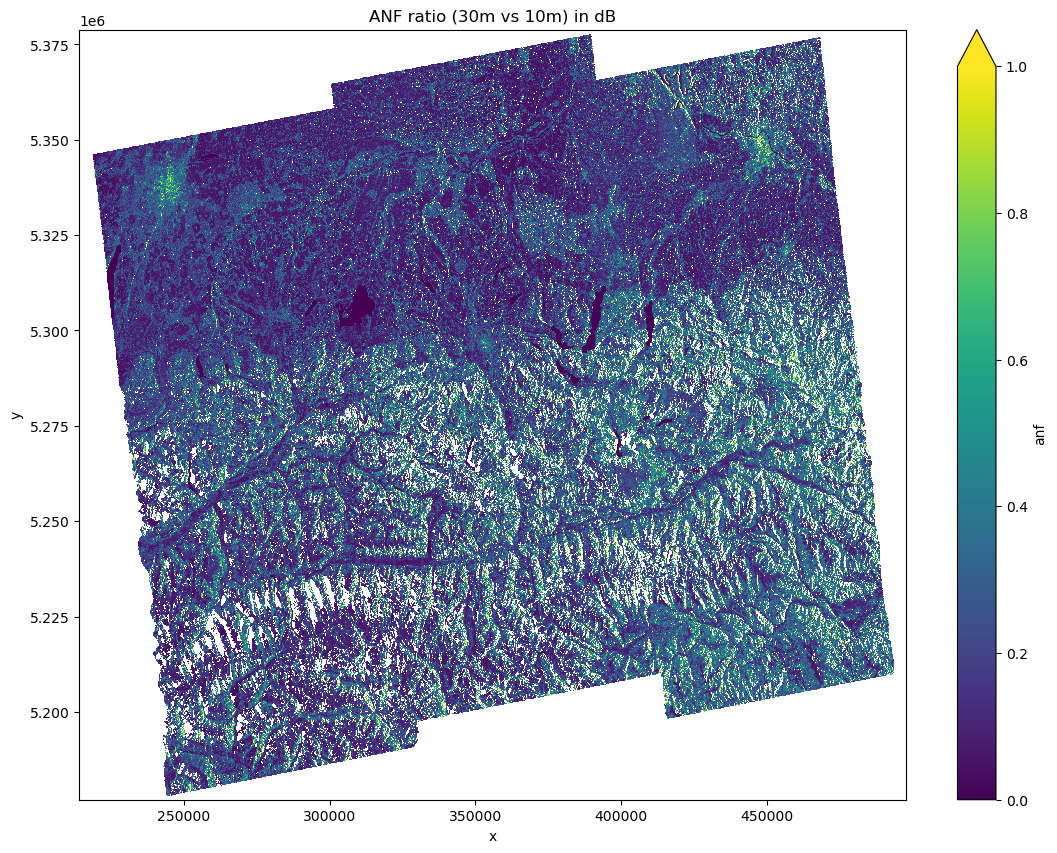
\includegraphics[width=0.9\textwidth]{Figures/nrb/anf_ratio_10m_vs_30m_dem.png}
  \caption{Difference in ANF (dB) between 10 m and 30 m DEMs. Larger deviations align with steep slopes, consistent with the first order model in \eqref{eq:ANF_first_ord}.}
  \label{fig:ANF_DIFF_DB_DEM}
\end{figure}

This comparison highlights spatial patterns of ANF error but does not identify which DEM yields the best NRB product. Definitive assessment requires radiometric analysis of actual SAR data acquired under multiple geometries (see Section~\ref{sec:nrb_stability_diff_geom}). At full resolution, speckle and image variability dominate these differences. Applying multilooking mitigates this issue, however at coarser resolutions the remaining differences are minor, serving mainly to reveal systematic bias.

\subsubsection{Slope Correction (ANF) and Orbital Tube Control}

The ANF also depends on the sensor’s precise position and attitude, which vary within the orbital tube. Even small deviations in the satellite’s orbit introduce errors in slant range geometry and thus in the computed incidence angle. Because Sentinel-1’s orbital tube is on the order of few hundreds of meters, the resulting ANF variations are relatively small, and in practice one can compute a single flattening layer for the nominal track and apply it to all scenes.

\paragraph{Theoretical model}
\label{sec:nrb_theoretical_model_orbital}

If an across-track baseline error \(B_{\perp}\) shifts the sensor off the nominal orbit, the resulting incidence angle perturbation is \(\delta\theta_i \approx B_{\perp}/R\), where \(R\) is the slant range distance. Starting from \eqref{eq:ANF_integral}, the corresponding ANF variation is
\begin{equation}
  \label{eq:ANF_first_ord_B_perp}
  \gamma_{\mathrm{ANF}_l}' 
  = \sum_{j \in J(l)} A_j w_{j,l} \cos\!\theta_{i_j} \,\bigl(1 - \tfrac{B_{\perp}}{R} \tan\!\theta_{i_j}\bigr),
\end{equation}
and its variance becomes
\begin{equation}
  \sigma^2_{\gamma_{\mathrm{ANF}_{B_\perp}}}
  = \gamma^2_{\mathrm{ANF}}
    \Bigl(\tfrac{\tan\!\theta_{\mathrm{max}}}{R}\Bigr)^{\!2}\,\sigma^2_{B_{\perp}}.
\end{equation}
Since \(R/dx\gg1\), DEM induced ANF errors dominate over orbital tube errors. Equation~\eqref{eq:ANF_first_ord_B_perp} also shows that a simple scaling, dependent on the angle, of the nominal ANF compensates for baseline variations up to a few kilometers.

\paragraph{Test on real data}

We validated these predictions using a stack of SAOCOM acquisitions over Naples, where the interferometric perpendicular baseline spans several kilometers. For each orbit realization, we computed the ground geometry ANF (no SAR image content involved) and then derived its spatial standard deviation. Figure~\ref{fig:ANF_STD_NAPLES} plots the measured \(\sigma_{\mathrm{ANF}}\): as expected, a correlation with the terrain slope is clearly visible: the variability of the ANF increases with slope, but in any case its variation is very small. The corresponding mean ANF across orbits is shown in Figure~\ref{fig:ANF_MEAN_NAPLES}.
Figure~\ref{fig:ANF_HISTOGRAM} shows a histogram of the maximum and minimum $ANF/ANF_{mean}$ ratios, which form two extremely narrow distributions, within $0.02$ dB.
\begin{figure}[h!]
  \centering
  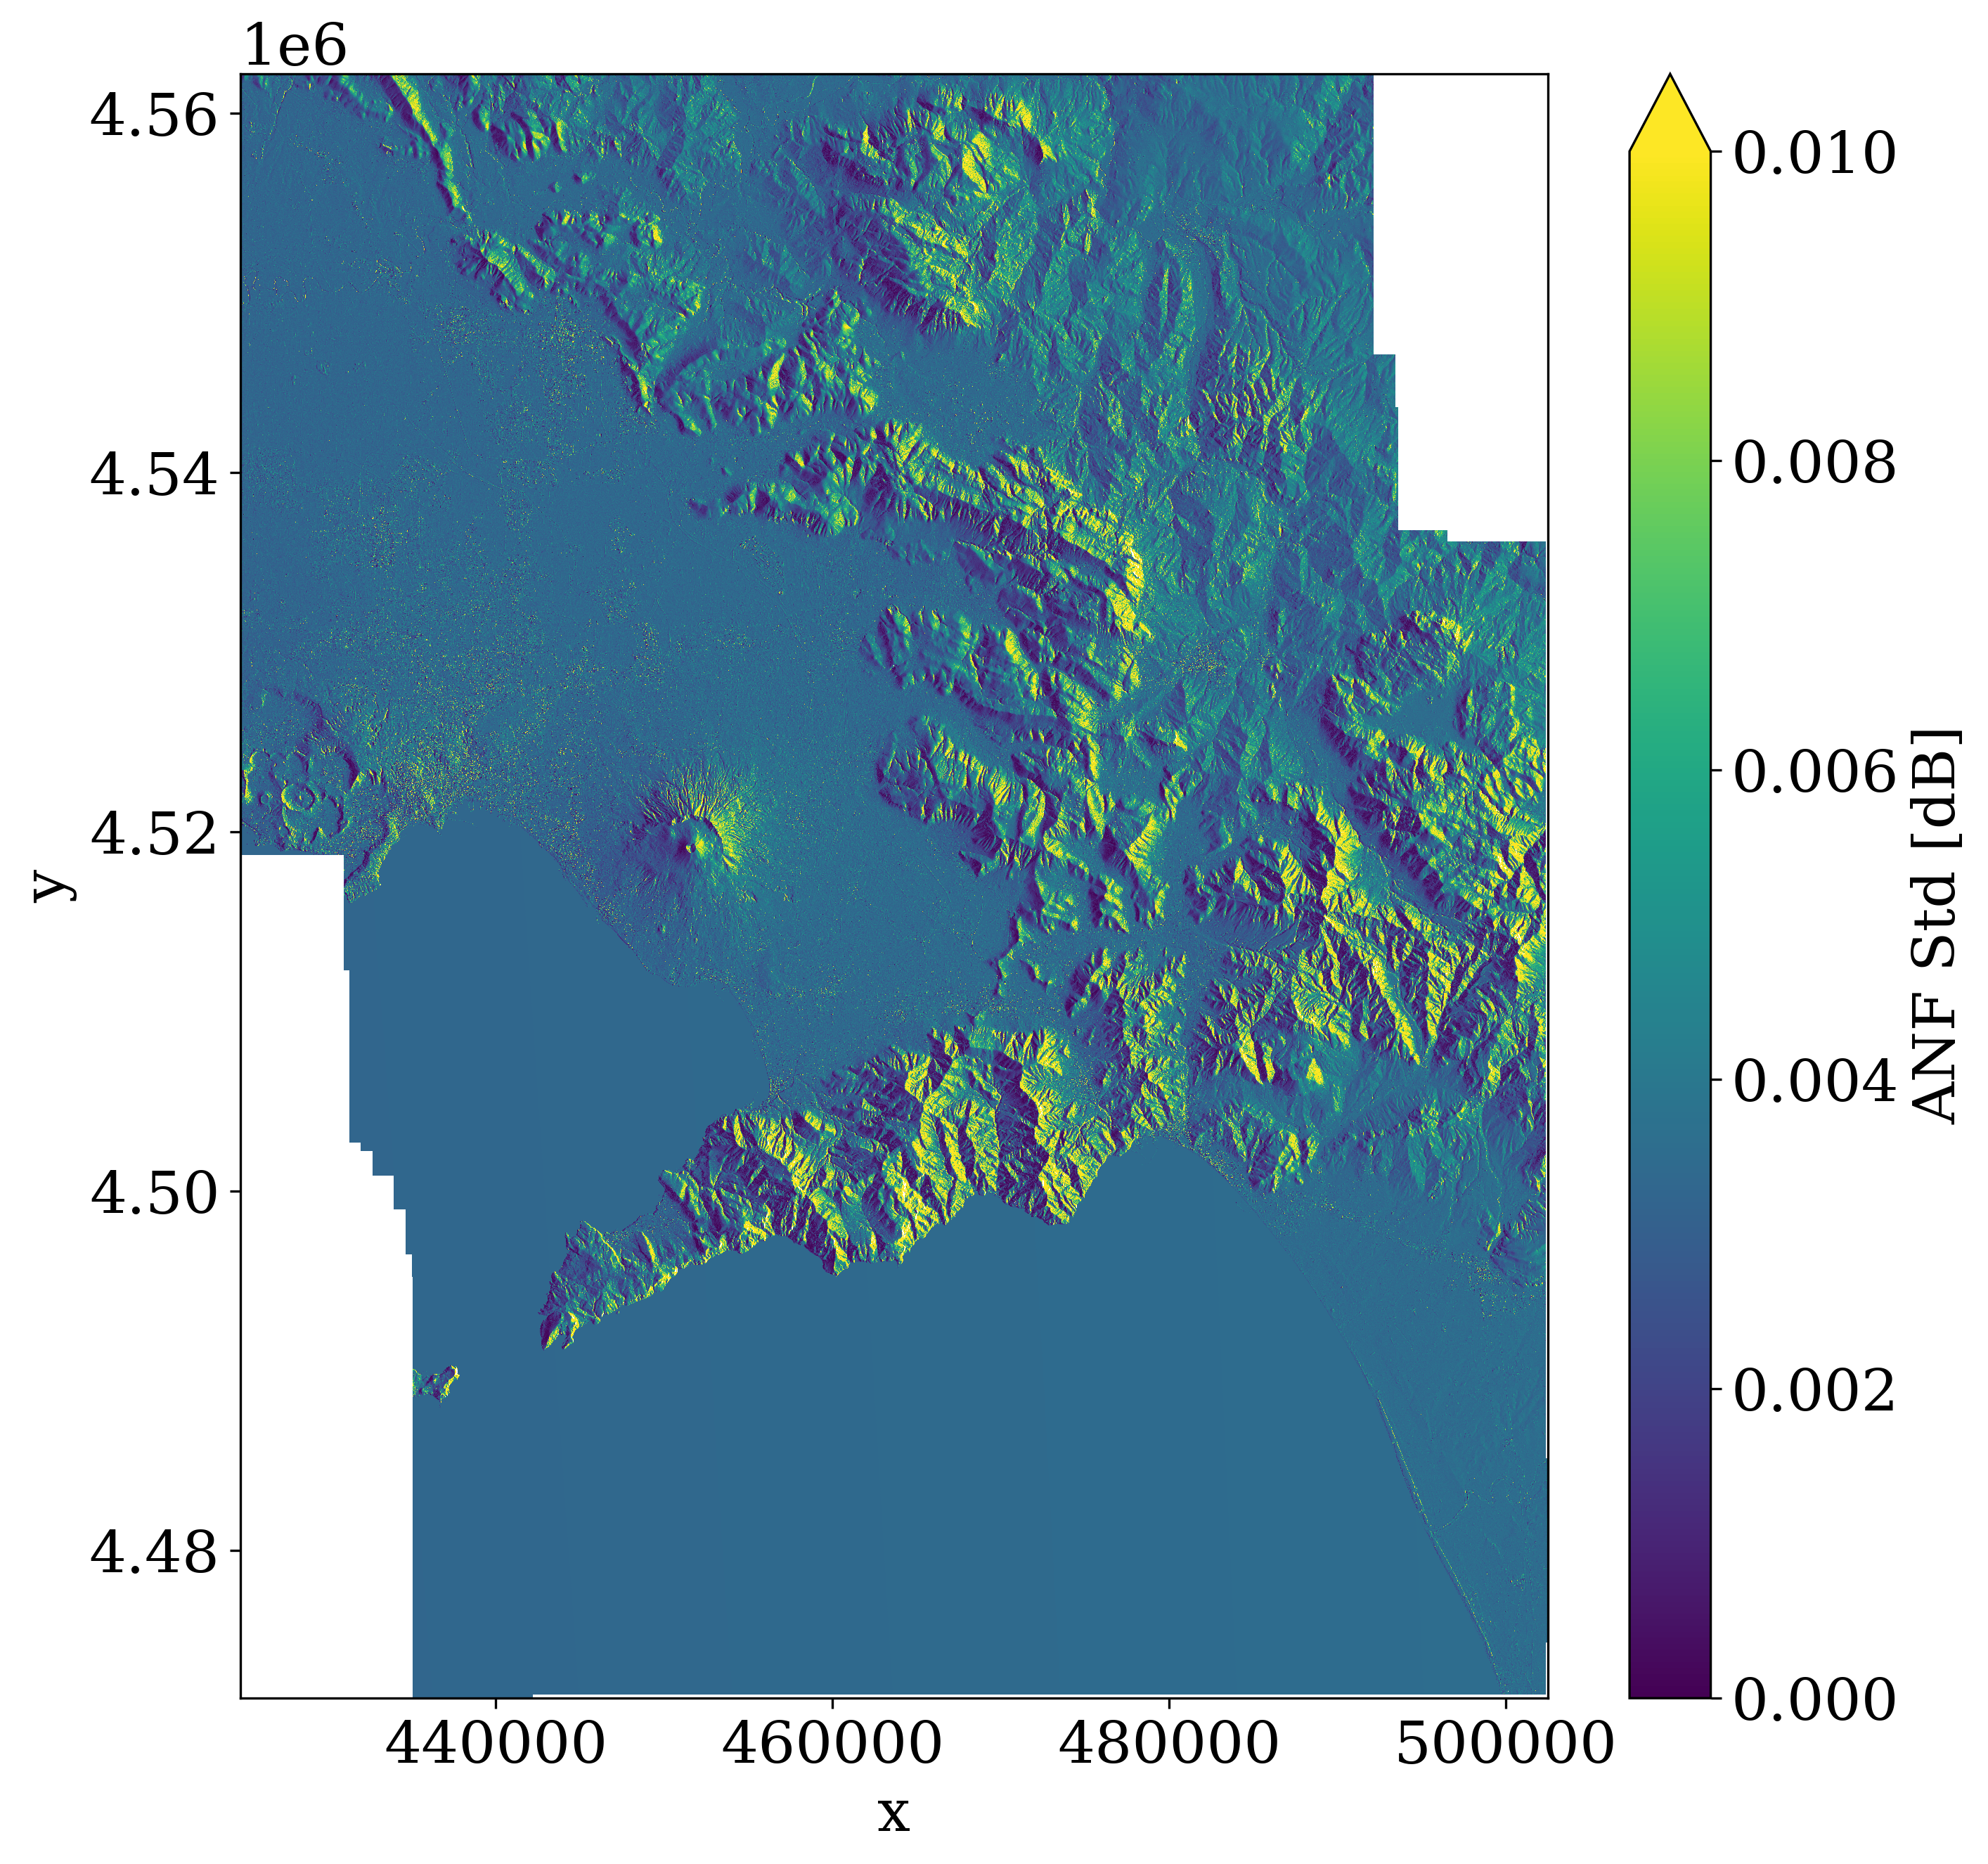
\includegraphics[width=0.9\textwidth]{Figures/nrb/anf_std_NAPLES.png}
  \caption{Standard deviation of ANF across multiple SAOCOM orbits over Naples. The image clearly shows that the ANF Variability increases with slope, in agreement with \eqref{eq:ANF_first_ord_B_perp}.}
  \label{fig:ANF_STD_NAPLES}
\end{figure}

\begin{figure}[h!]
  \centering
  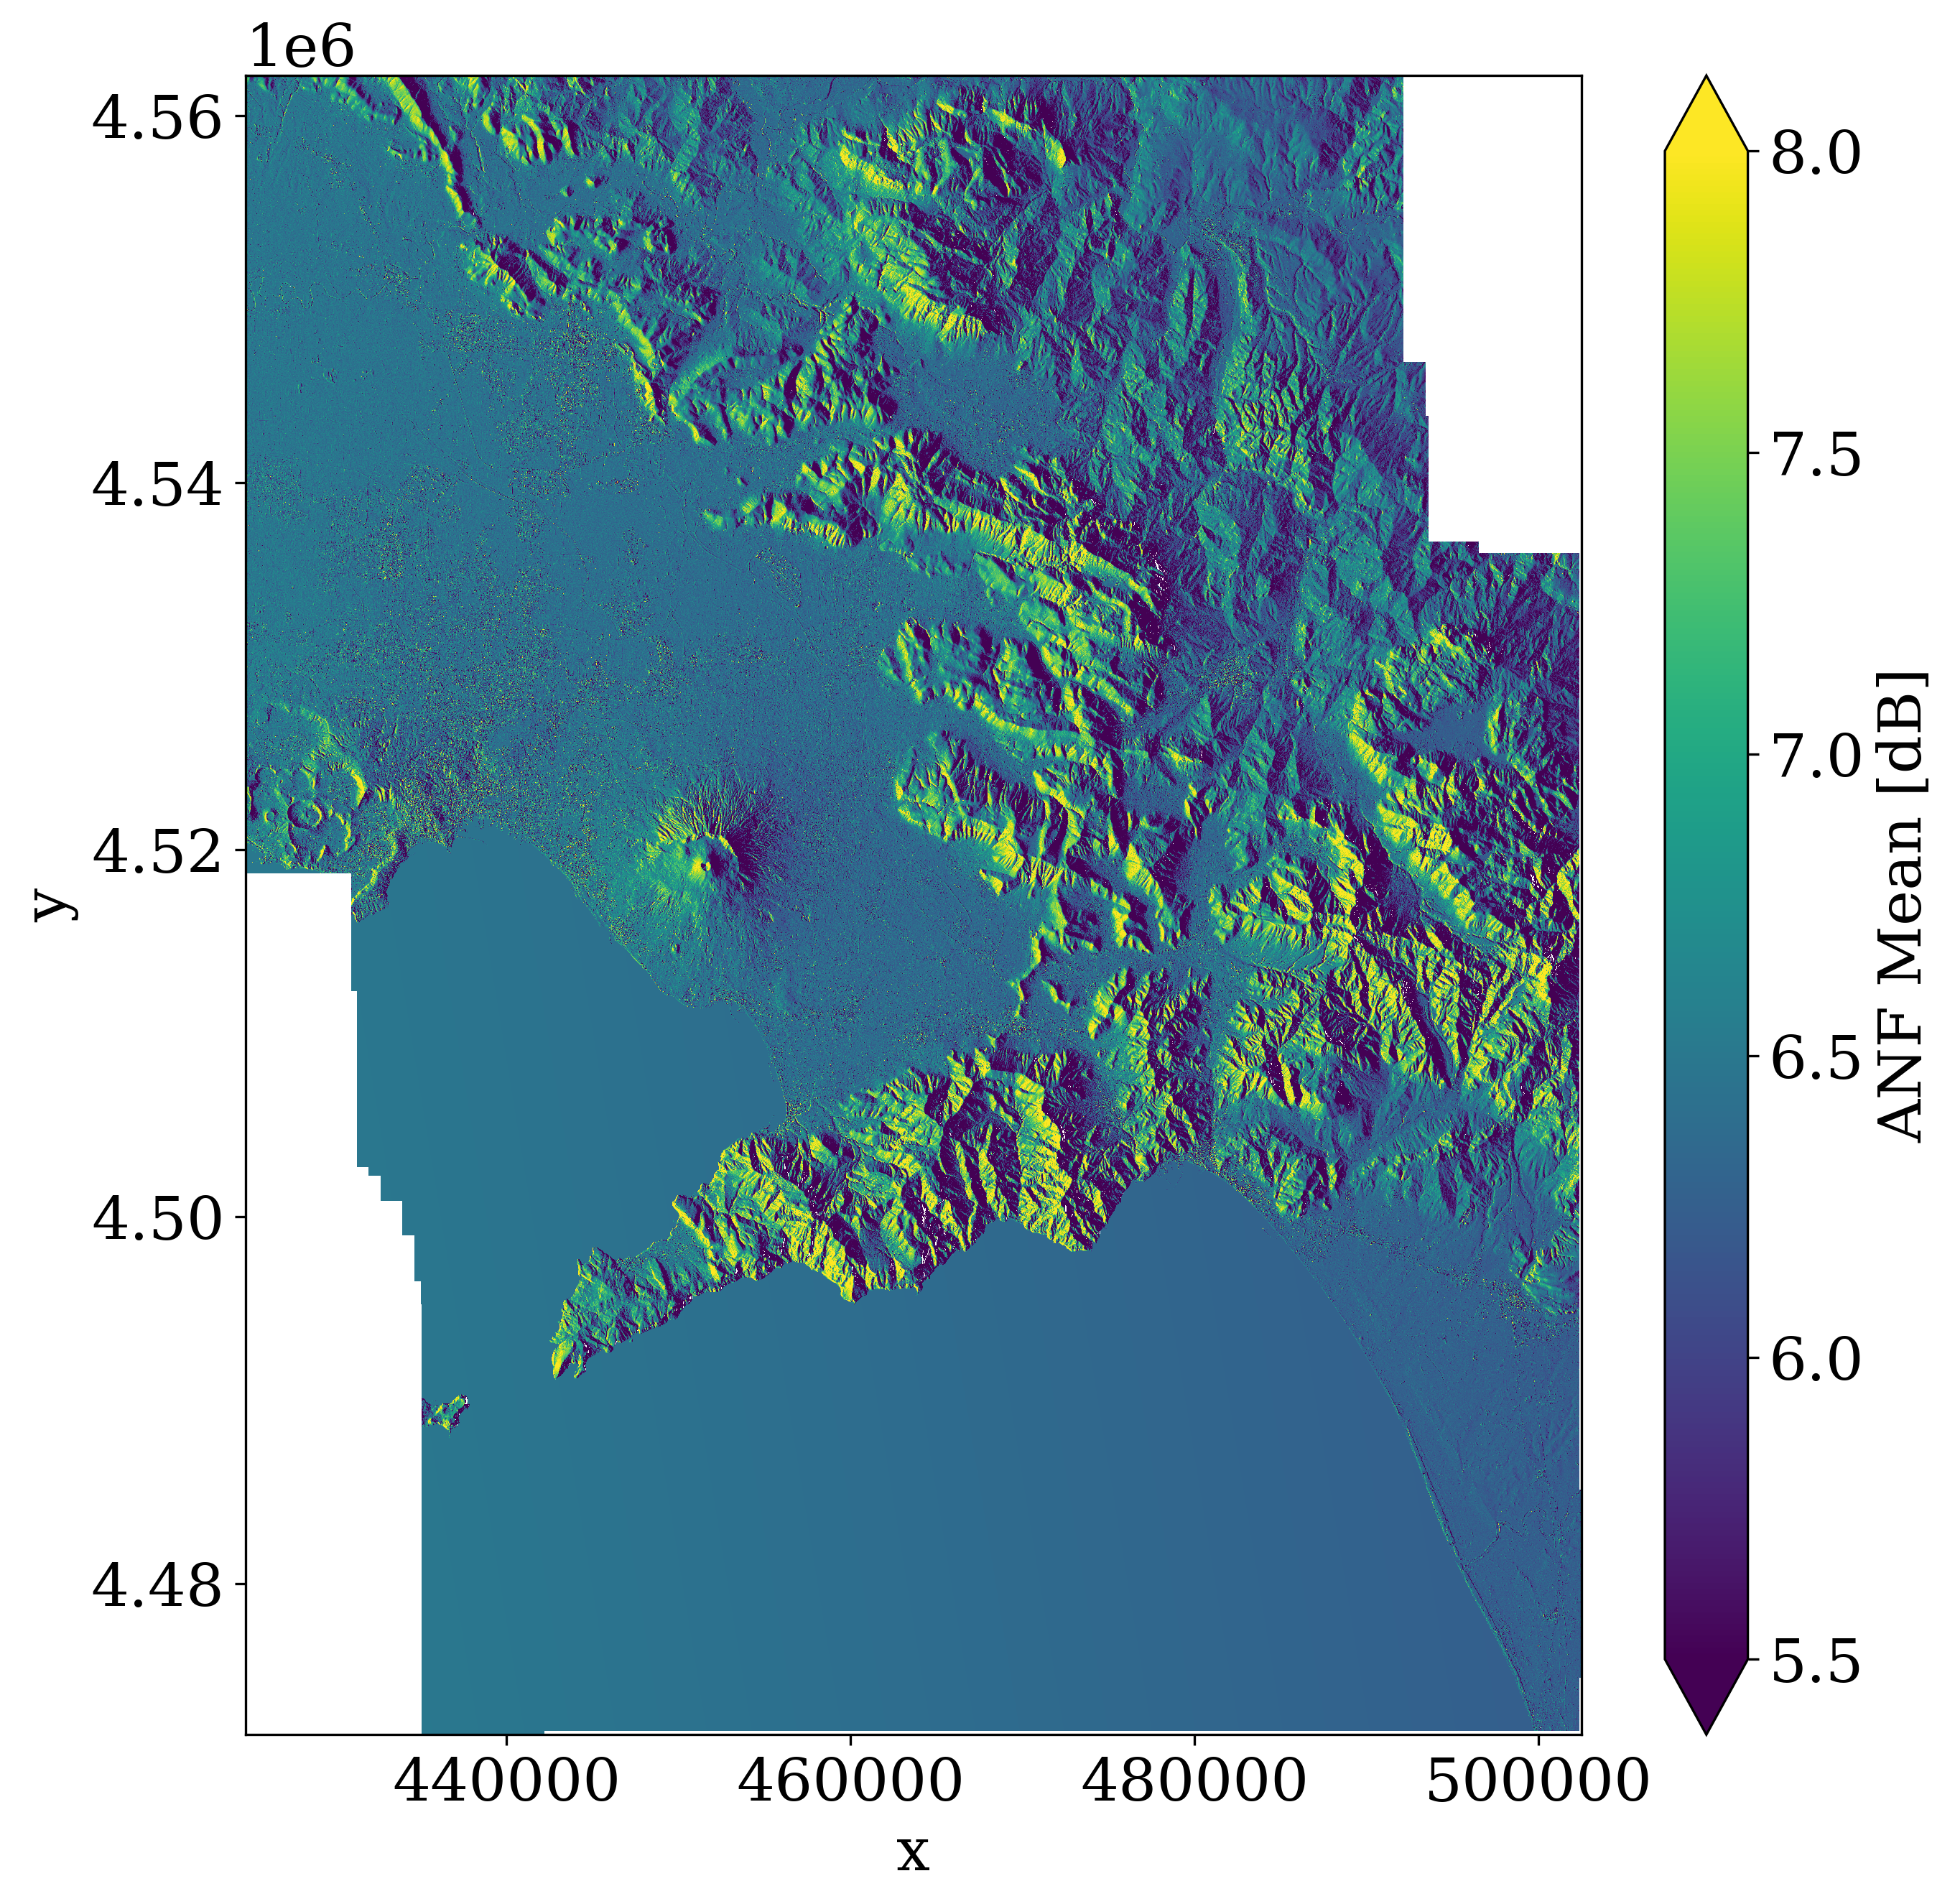
\includegraphics[width=0.9\textwidth]{Figures/nrb/anf_mean_NAPLES.png}
  \caption{Mean ANF across SAOCOM orbit realizations over Naples. The gradient reflects the cosine dependence in \eqref{eq:ANF}.}
  \label{fig:ANF_MEAN_NAPLES}
\end{figure}

\begin{figure}[h!]
  \centering
  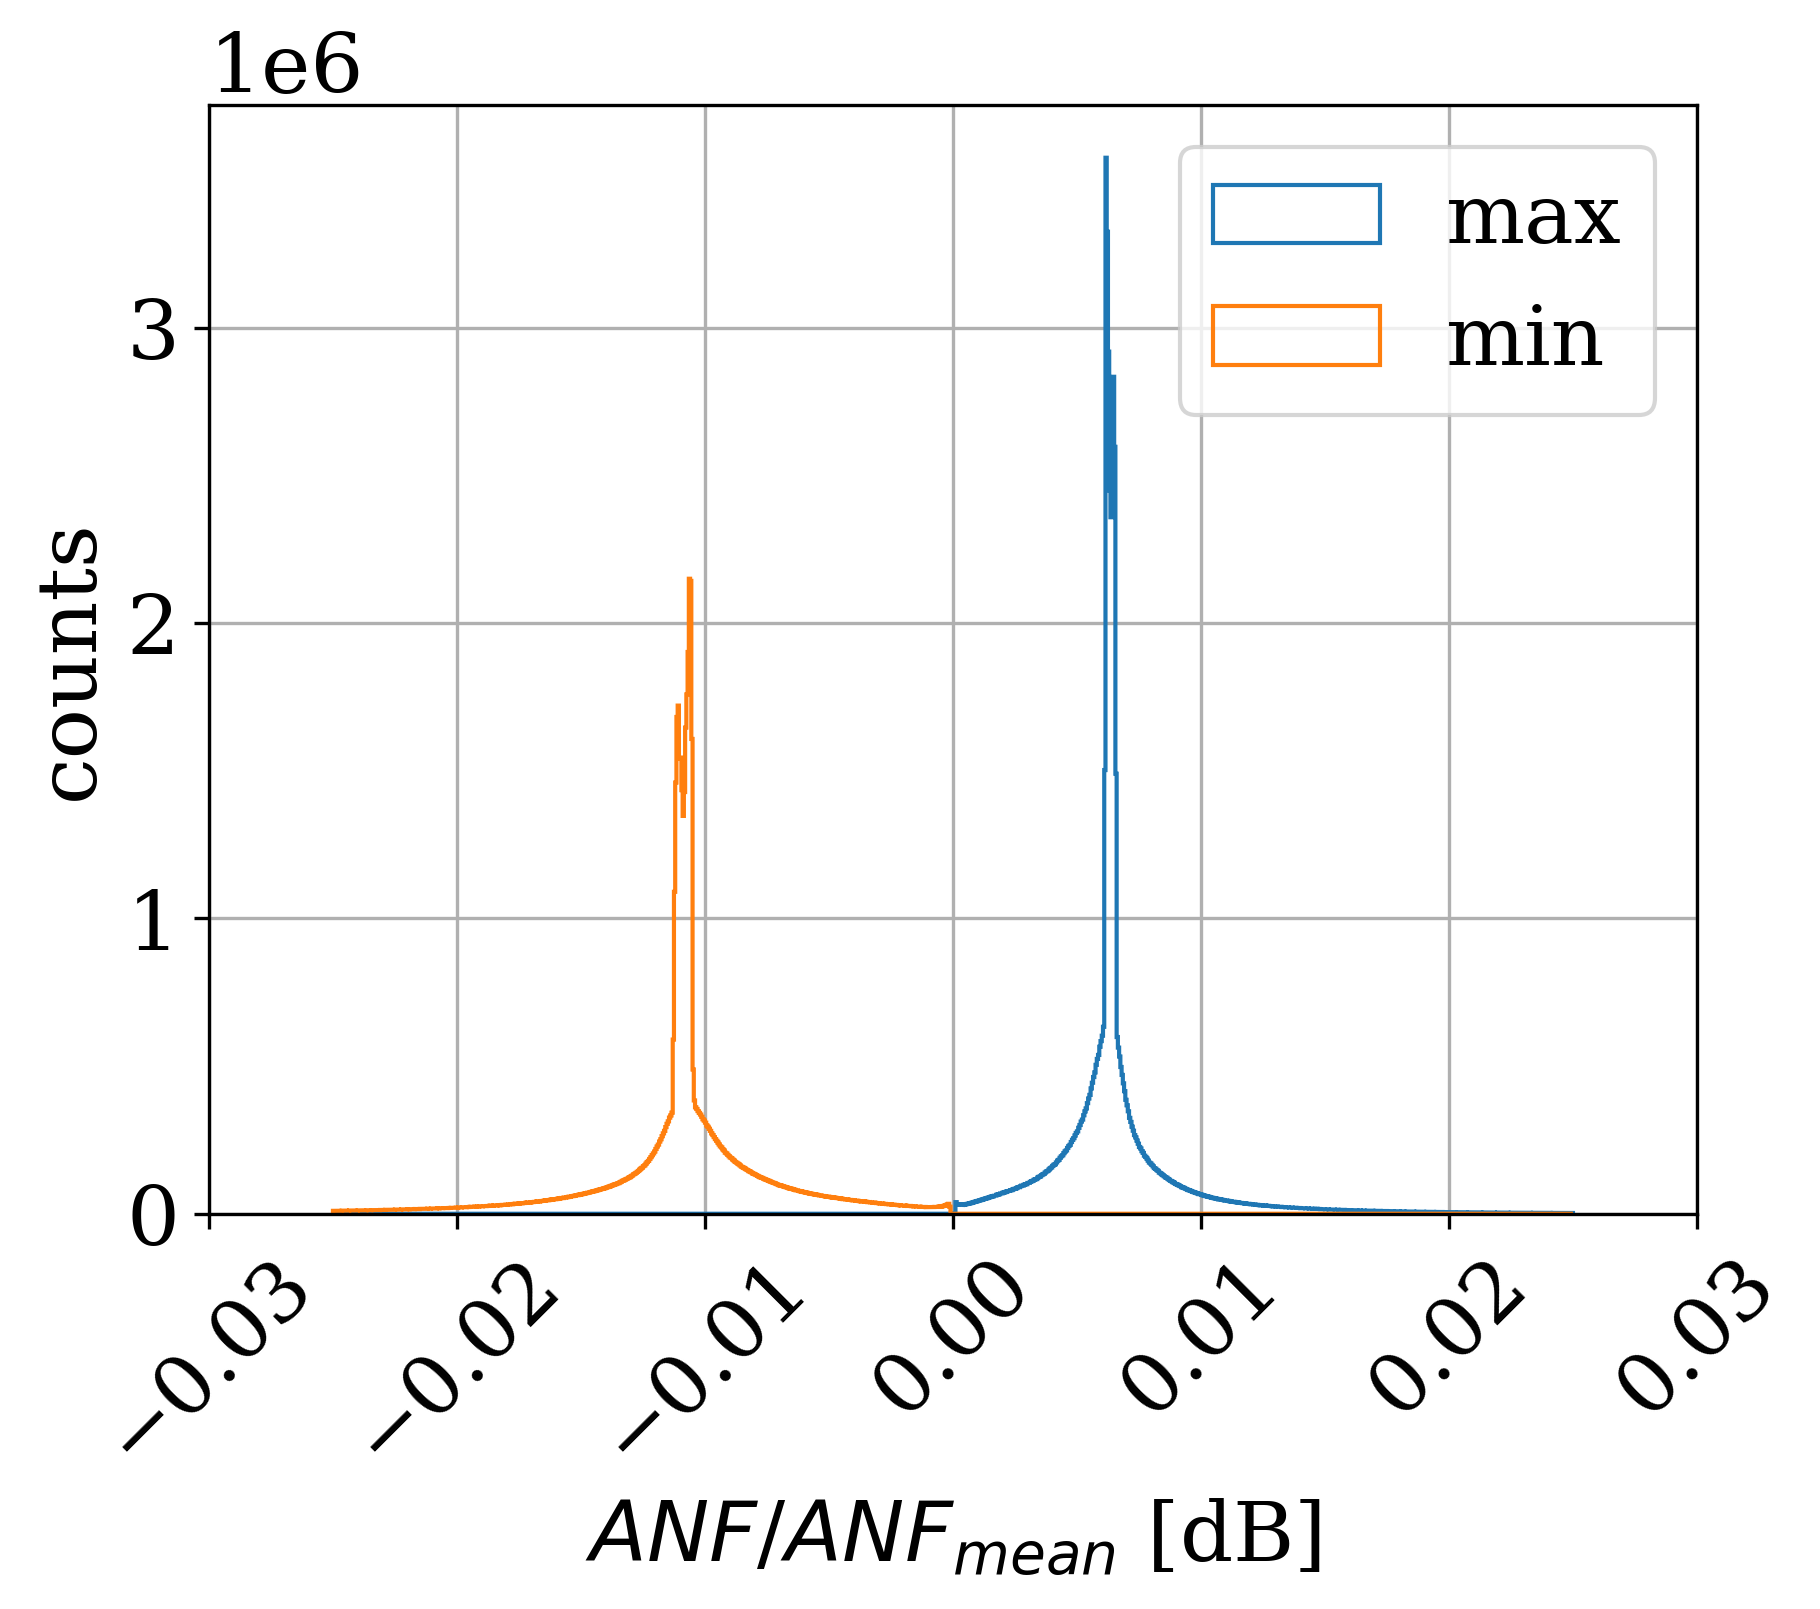
\includegraphics[width=0.9\textwidth]{Figures/nrb/histogram_ANF.png}
  \caption{Histogram of the maximum and minimum $ANF/ANF_{mean}$ ratio from SAOCOM orbit realizations over Naples. Both distributions are extremely narrow, within $0.02$ dB, indicating very low variance.}
  \label{fig:ANF_HISTOGRAM}
\end{figure}


Figure~\ref{fig:ANF_VS_BAS} shows the spatially averaged relative ANF (\(\Delta\mathrm{ANF}\)) versus \(|B_{\perp}|\). The near linear trend confirms the analytic scaling in \eqref{eq:ANF_first_ord_B_perp}, and even for baselines of 1 km the relative ANF error remains below 0.1 dB. Finally, Figure~\ref{fig:ANF_VS_INC_ANGLE} presents a two-dimensional scatter plot of ANF variability against incidence angle, with the theoretical first order curve overlaid. The close match validates our analytic model and suggests that a single, precomputed slope flattening layer, properly rescaled, suffices for an entire satellite track.

\begin{figure}[h!]
  \centering
  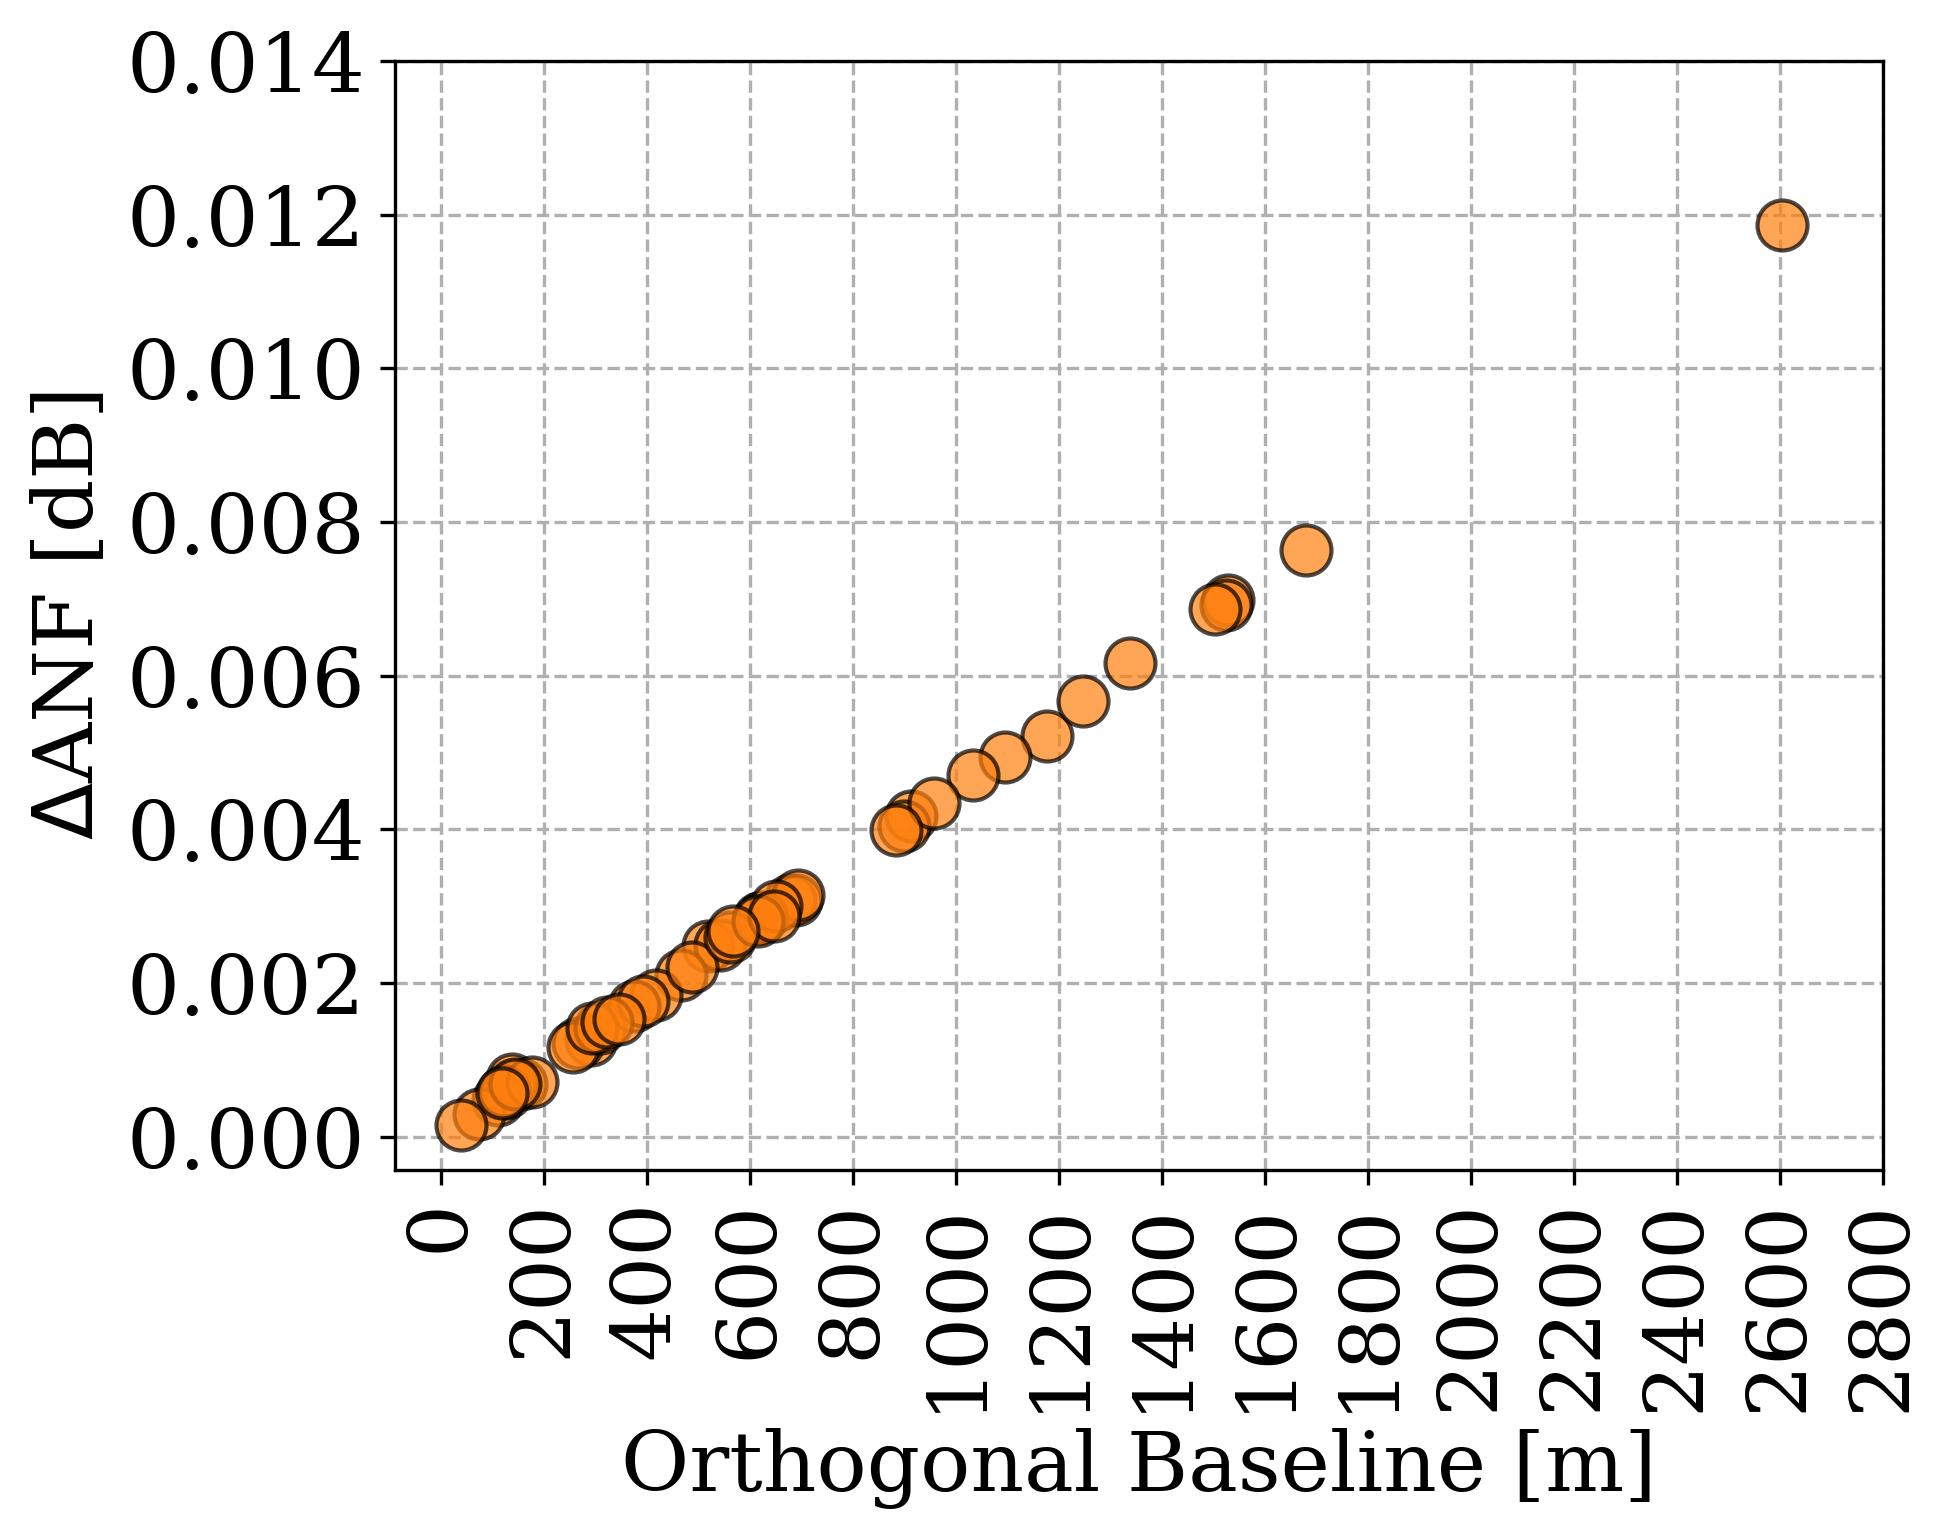
\includegraphics[width=0.9\textwidth]{Figures/nrb/baseline_division.png}
  \caption{Spatial average of \(\Delta\mathrm{ANF}\) versus the absolute perpendicular baseline \(|B_{\perp}|\). The linear increase matches the prediction of \eqref{eq:ANF_first_ord_B_perp}.}
  \label{fig:ANF_VS_BAS}
\end{figure}

\begin{figure}[h!]
  \centering
  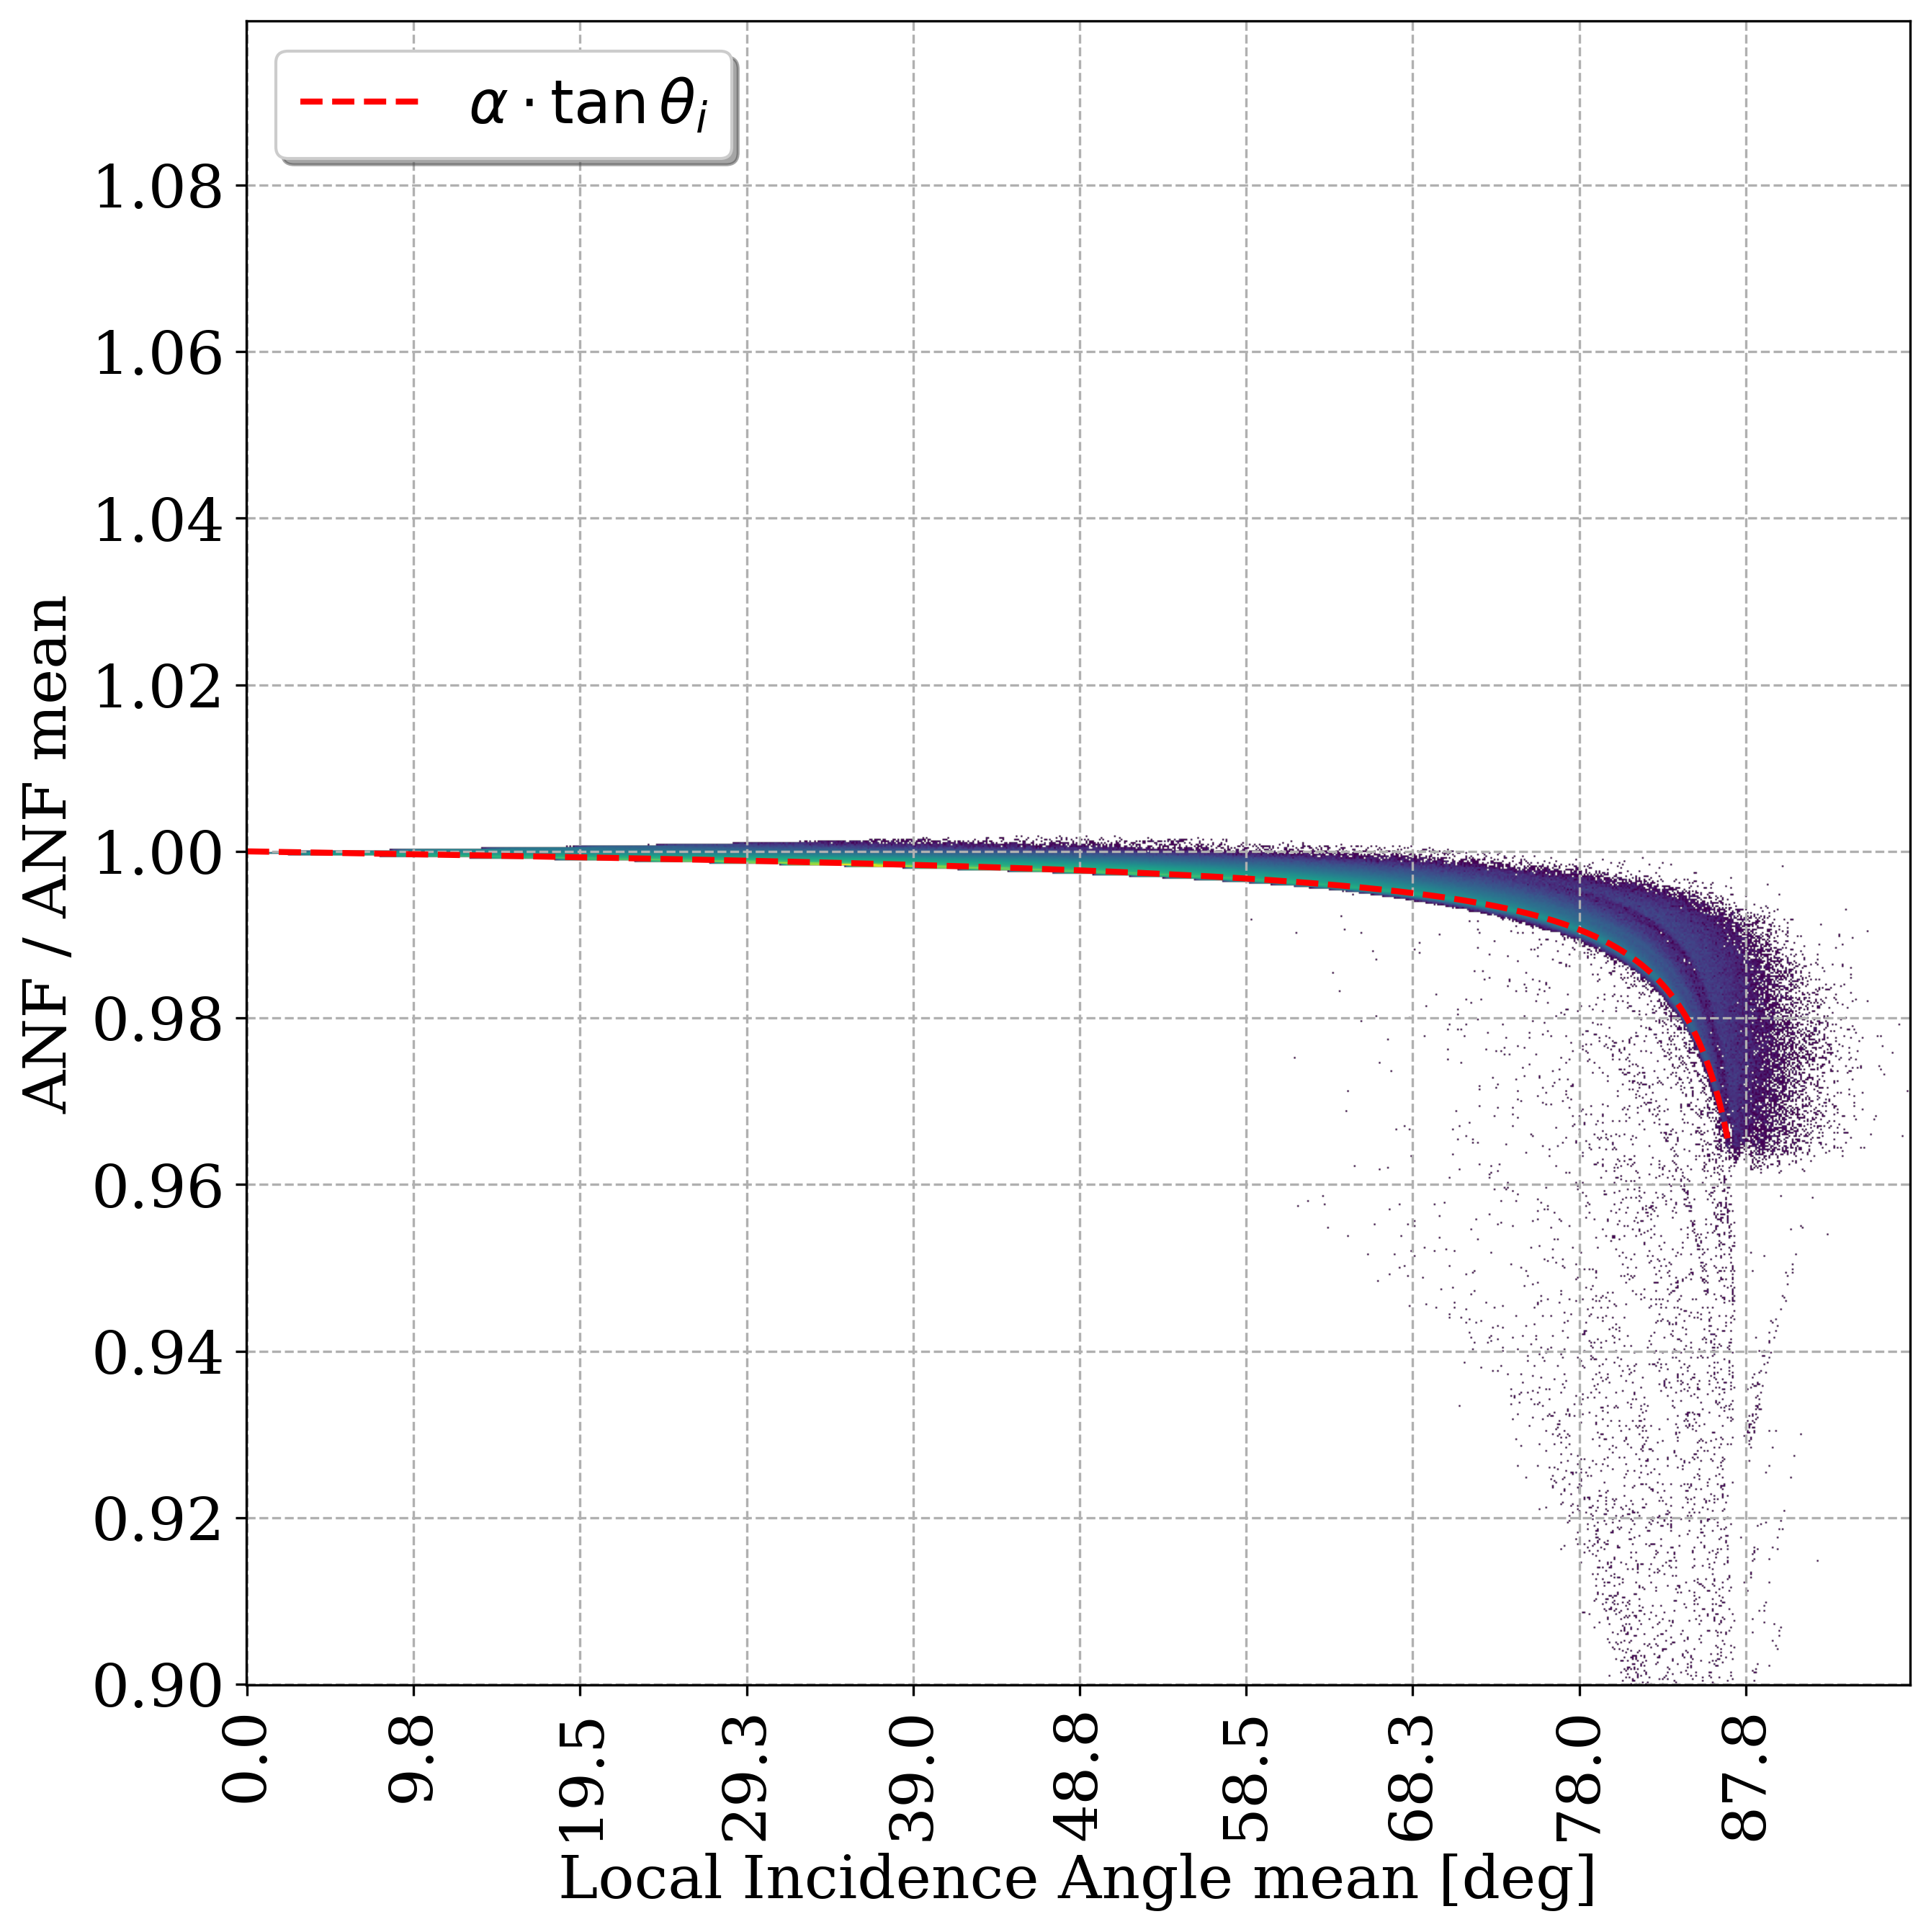
\includegraphics[width=0.9\textwidth]{Figures/nrb/anf_mean_over_lia.png}
  \caption{2D scatter of ANF variability versus local incidence angle. The dashed red line is the first order theoretical approximation from \eqref{eq:ANF_first_ord_B_perp}.}
  \label{fig:ANF_VS_INC_ANGLE}
\end{figure}

\subsection{Computational performance}
\label{sec:nrb_computation}
The generation of NRB products can be based on the processing of each single image independently, with the computation of the specific geometry in correspondence of every new acquisition, or on the processing of stack of images with a co-registration in radar geometry to align all the images with respect to a reference one and the slope flattening andf geocoding with a unique function computed in correspondence of the reference image.

In table \ref{tab:processing_time_single} the absolute time and the percentage of computational cost of the different processing steps with respect to the total amount processing time is reported for a single image. The test refers to an entire Sentinel-1 scene (27 bursts) acquired in IW mode in dual polarization.


\begin{table}[ht]
  \centering
  \caption{Processing time percentage cost vs the total processing time for single image.}
  \label{tab:processing_time_single}
  \begin{tabular}{lll}
    \hline
    Processing step & Processing time [s] & Cost percentage [\%] \\
    \hline
    DEM reprojection    & 63.5 & 9     \\
    Simulation    & 59.4 & 8    \\
    Rasterization  & 413.6 & 56      \\
    Mask shadow    & 108.2 & 15      \\
    Geocoding    & 71.1 & 10      \\
    Mosaic    & 25 & 3      \\
    \hline
  \end{tabular}
\end{table}

The two most time consuming steps are ``Rasterization'' and ``Mask Shadow''. It is worth noting that, by defining a reference geometry, these two steps can be executed only once.

Following this approach and including the image coregistration flow, the processing time percentages is reported in the table \ref{tab:processing_time_single}.

\begin{table}[ht]
  \centering
  \caption{Processing time percentage cost vs the total processing time for co-registration of a stack of 5 images.}
  \label{tab:processing_time_single}
  \begin{tabular}{lll}
    \hline
    Processing step & Processing time [s] & Cost percentage [\%]\\ 
    \hline
    DEM reprojection    & 63.5 & 3     \\
    Simulation   & 430.2 & 20      \\
    Rasterization  & 413.6  & 19      \\
    Mask shadow    & 108.2 & 5      \\
    Coreg   & 695.95 & 33      \\
    Geocoding    & 350 & 16      \\
    Mosaic    & 70.5 & 3      \\
    \hline
  \end{tabular}
\end{table}

Notice that the time to process 5 images is only 2.8 times the one necessary to process a single image with a significant cost reduction. 

\subsection{Criticalities and weakness}
\label{sec:nrb_criticalities}

The generation of NRB products is a well-established process. This type of product is produced routinely using Sentinel-1 data, where a model-based approach is sufficient to correct geometric distortions and compensate for terrain slope.

A critical factor is the alignment between the ANF (simulated backscattering) and the actual SAR image intensity. This alignment depends on the quality of the DEM as well as the accuracy of orbital data and timing. Therefore, it is essential to rely on precise orbital information and timing corrections to account for atmospheric delays (tropospheric and ionospheric).

With Sentinel-1 data, the primary challenge is the timeliness of the availability of these external inputs. For ROSE-L data, additional data-driven corrections are required to compensate for ionospheric effects.

Regarding output resolution, generating products at 10 m is feasible, but speckle becomes the main limiting factor. Based on analyses conducted on Sentinel-1 data, the effective number of looks is approximately 2 in flat areas, and the variability of the backscattering is dominated by speckle. If the final application does not require maximum resolution, lowering the output resolution may be advisable. In addition, this adjustment reduces computational cost proportionally to the increase in the size of the output cell.

The impact of input DEM resolution is primarily confined to areas with steep slopes. Using an area-based approach and comparing input DEM resolutions of 10 m and 30 m—while processing the same image and targeting a 10 m product resolution—the RMSD in steep-slope regions (e.g., the Alps) is less than 1 dB. The RMSD decreases rapidly as the output resolution is lowered.

Orbital tube control is not critical, and two possible mitigation strategies are available:
\begin{itemize} 
    \item \textbf{Independent processing of each image}: the area-based algorithm can be applied individually to each image. In this case, it is crucial to ensure the availability of precise orbital data and SAR image timing information in order to align the ANF with the actual image. 
    \item \textbf{Rescaling the ANF function}: the error in ANF determination can be expressed as a function of the interferometric baseline with respect to the reference geometry and the local incidence angle. By applying a correction specific to each image, it is possible to accurately compensate the ANF without requiring a full computation. 
\end{itemize}


\subsection{Notes on NRB multilook}
\label{sec:nrb_multilook}
Given not normalized weights at $ m $  meters resolution $ v^{m}_{qr} $ for each geographic grid pixel $ q $ and radar pixel $ r $.\\
The not normalized weights at $ n \times m $  meters resolution are given by:
\begin{align}
v^{n \times m}_{pr} = \sum_{q \in p}^{} v^{m}_{qr}
\end{align}
where $q \in p$ denotes all pixels with spacing $m$ that lie within the pixel $p$ with spacing $m \times n$.
The geocoded intensity at $m$ meters resolution is given by:
\begin{align}
g^m_q = \frac{\sum_{r} v^{m}_{qr} c_r}{\sum_{r} v^{m}_{qr}} =\frac{\tilde{g}^m_q}{n_q^m} 
\end{align}
where $c_r$ is the intensity of the radar pixel $r$ and $n_q^m$ is the number of looks of the geogrid pixel $q$.
Then, at $ n \times m $ resolution, the geocoded intensity can be expressed as:
\begin{align}
g^{n \times m}_p &= \frac{\sum_{r} v^{n \times m}_{pr} c_r}{\sum_{r} v^{n \times m}_{pr}} = \frac{\sum_{r}\sum_{q \in p}^{} v^{m}_{qr} c_r}{\sum_{r} \sum_{q \in p}^{} v^{m}_{qr}}=\frac{\sum_{q \in p}^{} \sum_{r}v^{m}_{qr} c_r}{\sum_{q \in p}^{}\sum_{r} v^{m}_{qr}}\\
&= \frac{\sum_{q \in p}^{} \tilde{g}^m_q}{\sum_{q \in p}^{}n_q^m} = \frac{\sum_{q \in p}^{} {g}^m_q \cdot n^m_q}{\sum_{q \in p}^{}n_q^m}
\end{align}

\subsection{Processors configurations}
\label{sec:nrb_proc_config}

\subsubsection{S1-RP}
The following parameters have been used:
\begin{itemize}
    \item chunks to be used during processing: \{"x": 1024, "y": 1024\}
    \item spacing of the resampled DEM: \{"x": 0.3 / 3600, "y": 0.3 / 3600\}
    \item apply\_flattening, whether to apply RTC flattening: True
    \item crs of the resampled DEM: 4326
    \item n\_jobs, number of workers to use: 16
    \item job\_memory, memory allocated for each worker: "16GB"
\end{itemize}
    
\subsubsection{Small C-Code}
Given the zip of a file\\"S1A\_IW\_SLC\_\_1SDV\_20190424T172321\_20190424T172348\_026935\_0307CD\_55E0.SAFE":
\begin{itemize}
    \item unzip the set of input products:  unzip\_list *.zip 
    \item Move each product into “superstructure” to hold the input product with intermediate and output RTC products: mvS1\_list *SAFE
    \item create a backscatter mosaic:
    \begin{itemize}
        \item pushd SLC-IW-20190424\_172321-026935
        \item topsmosBeta SLC-IW-20190424\_172321-026935 1
        \item popd
    \end{itemize}
    \item Run script to create RTC products from a Sentinel-1 IW SLC product:\\ rtcS1slc\_list SLC-IW-20190424\_172321-026935\\
    Line 22 of the rtcS1slc\_list script has been modified in:\\ rtcS1\_dhm\_slc \$f 1 \$UZHRTC\_DIR/DEM/dem 0.3s 1 1000
\end{itemize}
\subsubsection{OPERA-ISCE3}
\begin{itemize}
    \item create a new conda environment: conda create -n RTC -c conda-forge python=3.11.12
    \item activate your conda environment: conda activate RTC
    \item download the source code:\\ git clone -b v1.0.2 https://github.com/opera-adt/RTC.git
    \item install isce3: conda install -c conda-forge isce3==0.15.0
    \item download s1-reader:\\
    git clone -b v0.2.4 https://github.com/isce-framework/s1-reader.git
    \item install s1-reader:\\conda env update -n RTC -f s1-reader/environment.yaml\\
    python -m pip install ./s1-reader
    \item install RTC:
    python -m pip install ./RTC
    \item launch the software: rtc\_s1.py rtc\_s1\_.yaml
\end{itemize}
An example of the configuration file used is provided below:
\lstinputlisting[language=yaml]{Figures/nrb/rtc_s1.yaml}

\section{Polarimetric products (POL)}
\label{sec:pol}

The \acs{pol} \acs{ard} products considered in this project correspond to the polarimetric covariance matrix, which can be provided in radar coordinates (\acs{cov}) or in geographical coordinates (\acs{gcov}), i.e. after geocoding. The inputs required to generate these products correspond to individual \acs{slc} images or to previously generated \acs{cslc} products. In both cases, the processing required to compute each entry of the matrix is totally equivalent to what is done to produce \acs{nrb} data, so the reader is referred to \autoref{sec:nrb} for consulting the models and computational performance involved in such a product.

Since the \acs{pol} products involve more than one input polarimetric channel, the extension of the processing from \acs{nrb} to \acs{pol} must comply with the following rules:
\begin{itemize}
    \item When the input data is in \acs{cslc} form, the same co-registration grid (offsets of the secondary images with respect to the primary image) and interpolation must have been applied to all polarimetric channels. The common rule consists in computing the co-registration grid using only one channel (usually a co-polar one, i.e. VV or HH), and then applying it to all channels available.
    \item The same processing, i.e. the same algorithms, options and parameters (e.g. size of kernel), must be used for computing all entries of the matrix.
    \item Any spatial filtering or multi-look should be applied in radar coordinates, i.e. before geocoding, for preserving all the polarimetric information.
    \item The diagonal entries of the covariance matrix correspond to the backscattering coefficient of the individual polarimetric channels, and thus they are positive real numbers. However, the off-diagonal elements of the matrix are formed as products of the \acs{slc} values of different channels and, thus, they are complex values. Therefore, the implementation must take into account this difference in the type of data. 
\end{itemize}

In addition, the \acs{nrb} products are usually generated with a small equivalent number of looks (\acs{enl}) because they aim at preserving as much spatial resolution as possible. However, due to the higher dimensionality of the covariance matrix, the \acs{enl} required to properly estimate the covariance matrix is much larger than in the \acs{nrb} case. Because of that, an additional spatial filtering or multi-look is usually applied, hence changing the workflow with respect to a conventional \acs{nrb}. In fact, this is the main reason for providing also the \acs{cov} product, as the end user will be able to apply the spatial filtering required in radar coordinates. The \acs{cov} product will include a layer with a look-up table, or equivalent information, to geocode the result of the spatial filter, i.e. to transform it into a \acs{gcov} product, which is directly usable as an \acs{ard}.

\subsection{Evaluation criteria}
\label{sec:pol_criteria}

Apart from the impact of the spatial filtering or multi-looking, the conversion from a \acs{slc} or \acs{cslc} product to a \acs{pol} product does not entail any difference with respect to the conversion to \acs{nrb}. In other words, the generation of a \acs{pol} product must be evaluated in the same way as the generation of \acs{nrb}.

In order to stress the relevance of the equivalent number of looks (\acs{enl}) in the polarimetric case, which is more demanding than the single-pol case, in this section we illustrate the \acs{enl} provided by the different processing strategies, and its impact on polarimetric features derived from the resulting products.

\autoref{fig:pol_enl} shows the empirical estimates of \acs{enl} for two processing approaches: without multi-looking or spatial filtering (denoted as Shiroma), and with multi-looking for different window sizes (azimuth $\times$ range). The estimation of ENL from the output image is computed using the following expression~\cite{lee_intensity_1994}:
\begin{equation}
\text{ENL} = \frac{\hat{I}^2}{\sigma_I^2}
\end{equation}
where $\hat{I}$ and $\sigma_I^2$ denote the mean and the variance, respectively, of an intensity image (i.e. backscattering coefficient).
For this purpose, a homogeneous area on the scene is selected, which in this case corresponds to the sea.

\begin{figure}[ht!]
\centering
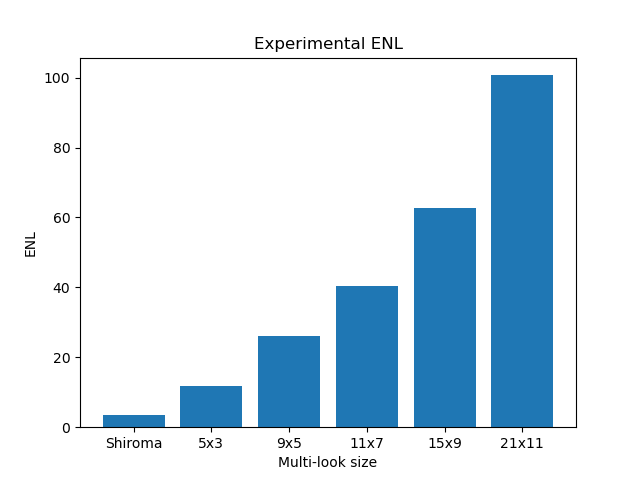
\includegraphics[width=0.8\textwidth]{Figures/pol/pol_enl_vs_multilook.png}
\caption{Equivalent number of looks (\acs{enl}) for two processing strategies: without multi-looking (denoted as Shiroma) and with multi-look for a set of window sizes (azimuth $\times$ range). Measurements are carried out with a dual-pol stripmap SAOCOM image over Naples (DSC pass, S4 beam) acquired on 28-02-2021. \acs{enl} is estimated empirically over a homogeneous area on the sea.}
\label{fig:pol_enl}
\end{figure}

The values shown in \autoref{fig:pol_enl} demonstrate that, due to the typical oversampling of \acs{sar} images, the number of looks is much smaller than the number of samples employed to compute averages in the multi-looking. In addition, it must be noted that the \acs{enl} value provided without multi-look, i.e. using only the geocoding step defined in~\cite{Shiroma2022}, is just 3.5 over this flat area. The \acs{enl} value in slopes facing the radar is much smaller, hence compromising the statistical significance of measures derived from the polarimetric covariance matrix.  

To assess the impact of the available \acs{enl} upon parameters derived from the \acs{pol} products, we show here the polarimetric entropy, which is widely used for scene characterisation and classification~\cite{Hajnsek2021}. 
For dual-pol data, polarimetric entropy $H$ is defined as:
\begin{equation}
    H = - \sum_{i=1}^2 p_i \cdot \log_2 p_i
\end{equation}
where
\begin{equation}
    p_i = \frac{\lambda_i}{\lambda_1 + \lambda_2},
\end{equation}
and $\lambda_1$ and $\lambda_2$ are the two eigenvalues of the dual-pol covariance matrix. A low entropy (close to 0) denotes the presence of a dominant scattering mechanism, whereas a high value (close to 1) represents a non-defined polarimetric response from the scene.

\autoref{fig:pol_entropy} shows the images of dual-pol entropy computed from the \acs{gcov} products pre-processed using Shiroma's approach and two different multi-look sizes. Entropy is generally low over the sea surface because its backscatter is dominated by a surface component, whereas it is very high over forested areas. Notably, there is a extremely high entropy zone in the lower left corner of the image, which corresponds to very calm water close to Ischia island. In this region the backscattering level is very close to the noise level, and hence the very high entropy. 

\begin{figure}[ht!]
\centering
\begin{tabular}{cc}
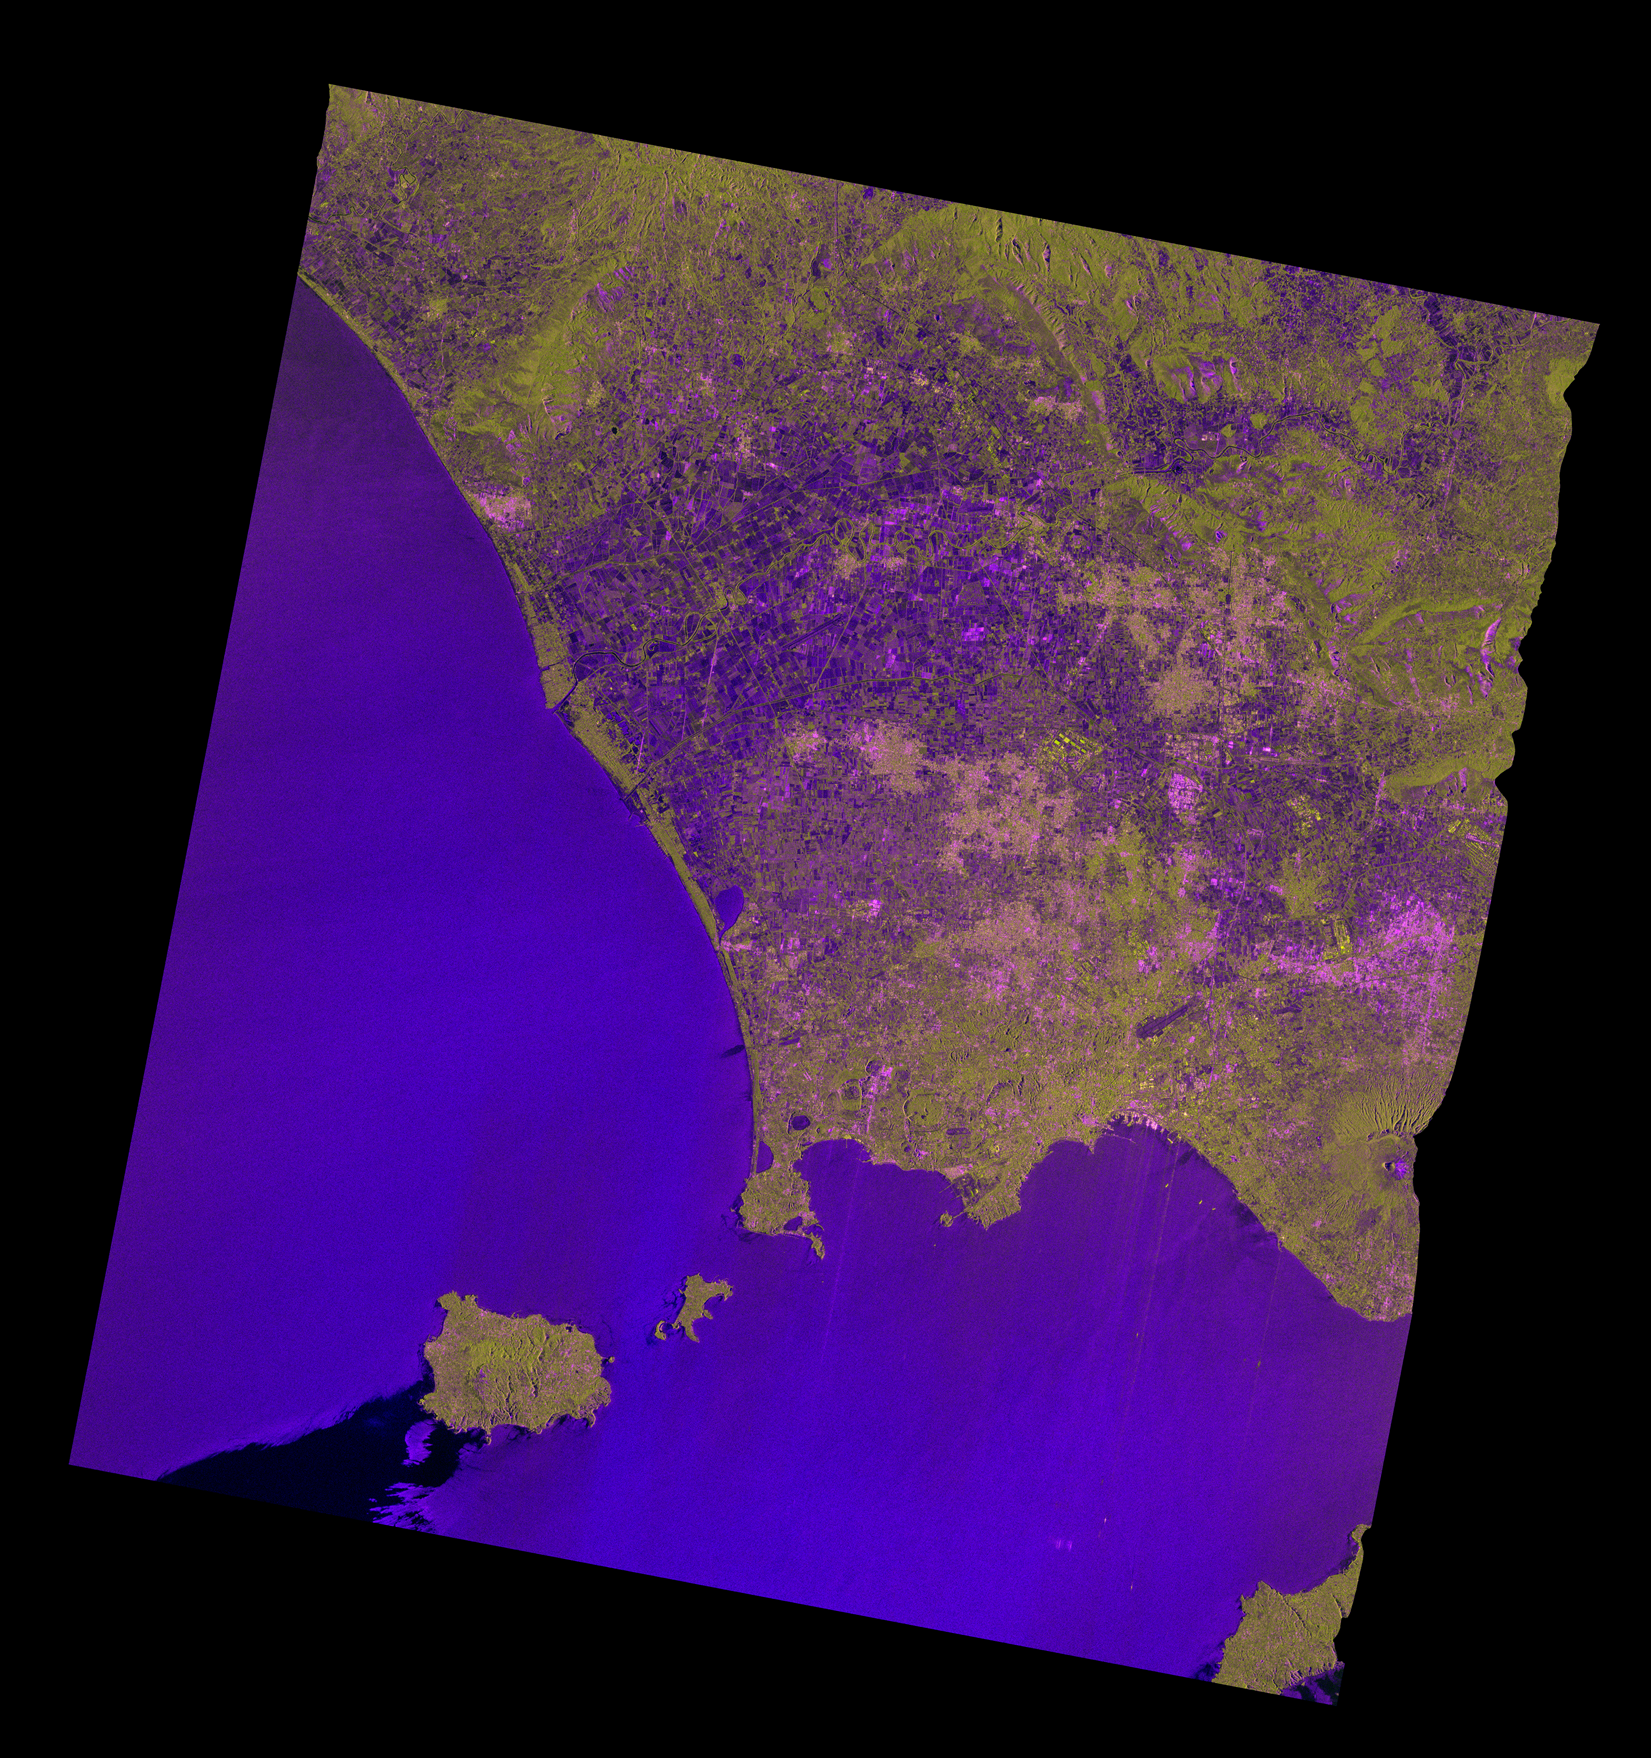
\includegraphics[width=0.35\textwidth]{Figures/pol/GCOV_LinearRGB_lowres.png}
 & 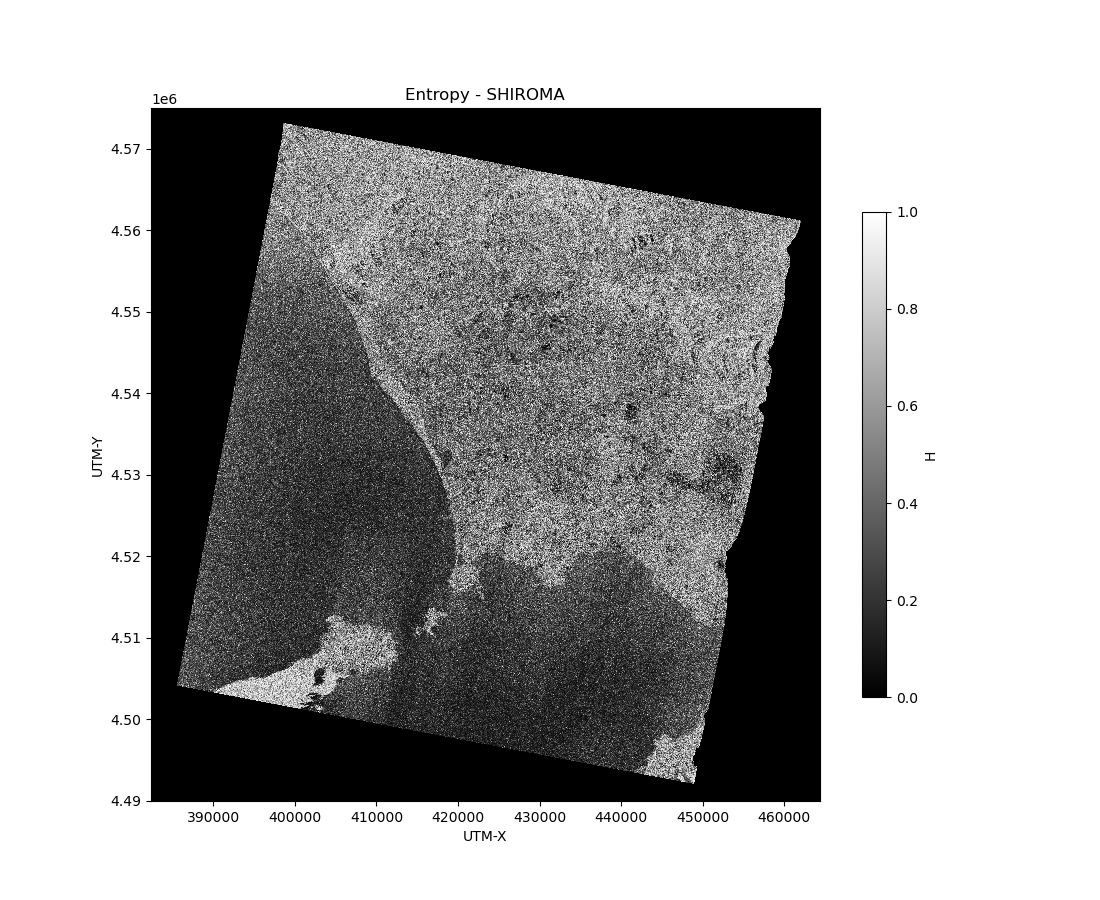
\includegraphics[width=0.5\textwidth]{Figures/pol/H_Shiroma.png}
 \\
(a) & (b) \\
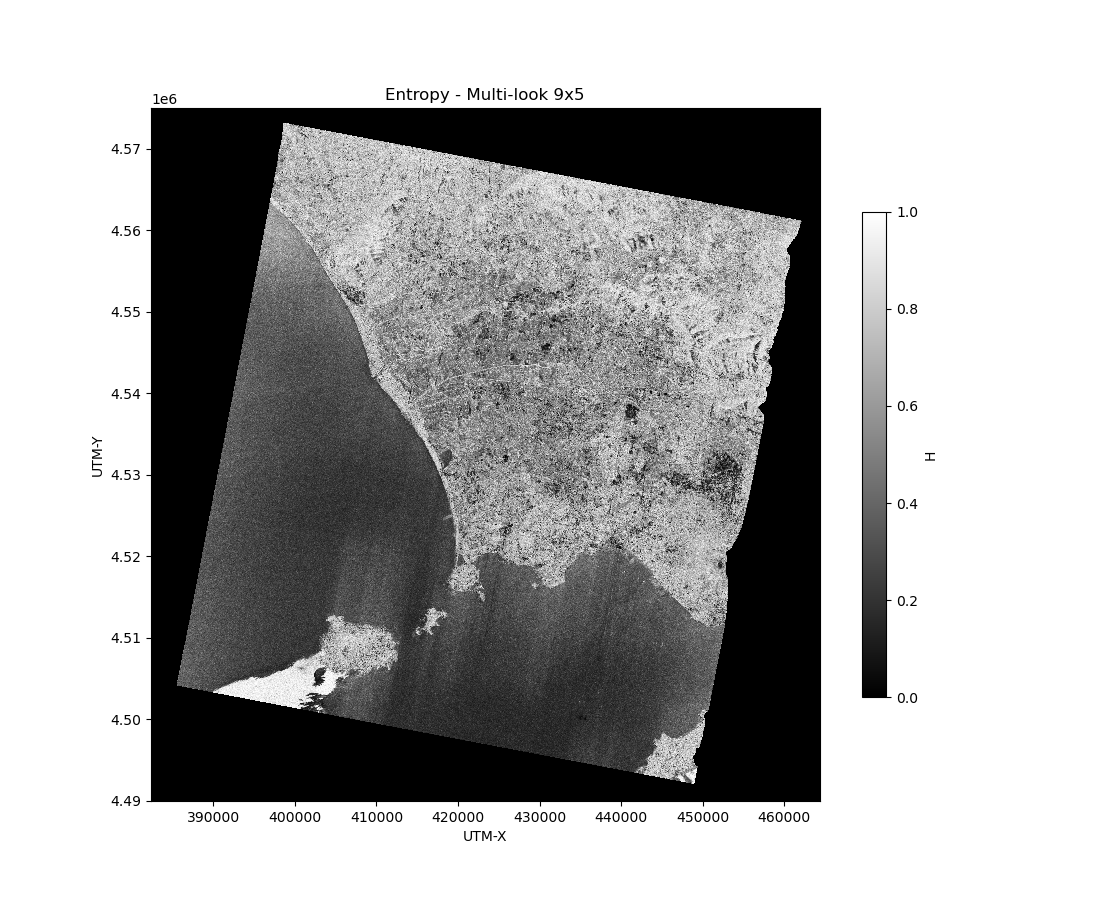
\includegraphics[width=0.5\textwidth]{Figures/pol/H_9x5.png}
 & 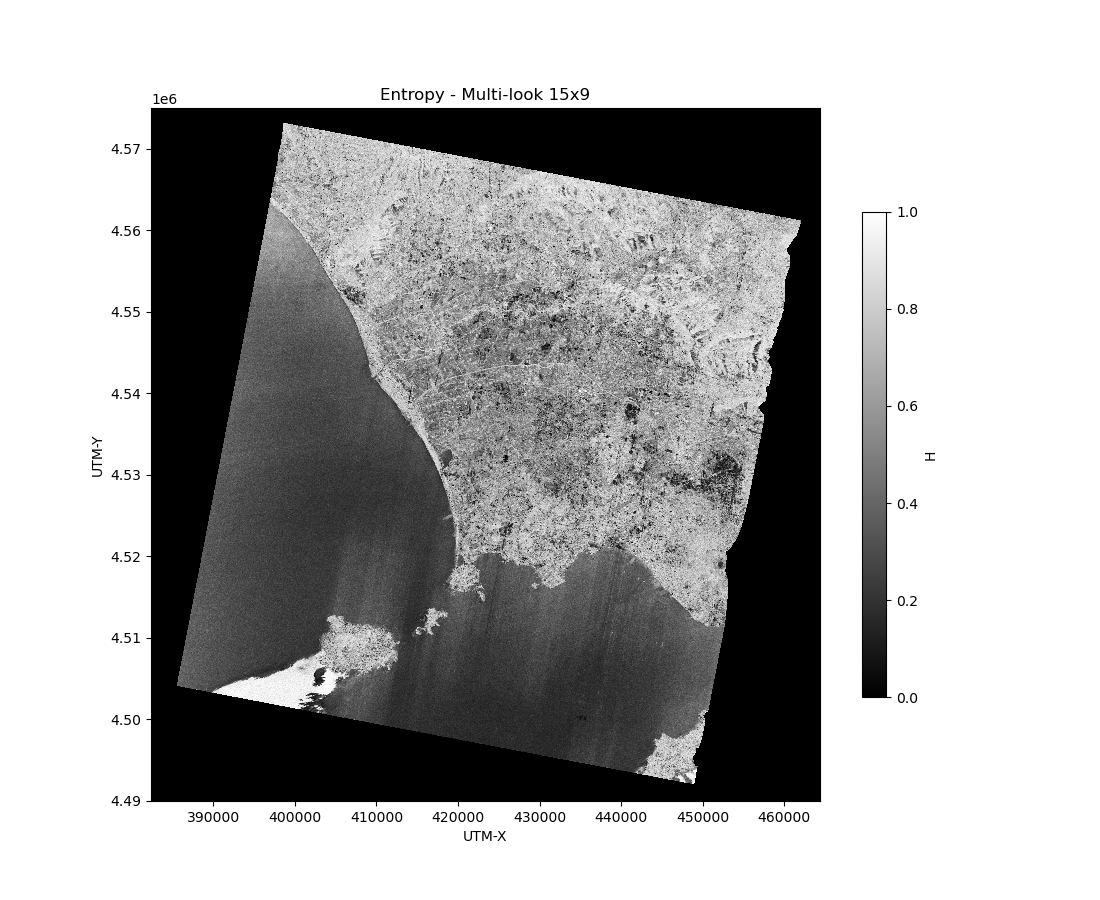
\includegraphics[width=0.5\textwidth]{Figures/pol/H_15x9.png}
 \\
(c) & (d)
\end{tabular}
\caption{Comparison of the dual-pol entropy computed for various processing options, using a dual-pol stripmap SAOCOM image over Naples (DSC pass, S4 beam) acquired on 28-02-2021. The RGB false colour composite is shown in (a). Images of entropy derived from the data pre-processed using: (b) Shiroma's approach, (c) 9x5 Multi-look, and (d) 15x9 Multi-look. }
\label{fig:pol_entropy}
\end{figure}

The computation of entropy from the sampled covariance matrix is known to be underestimated, being the bias more pronounced for higher entropies and for lower values \acs{enl}~\cite{LopezMartinez2005}. As a result, the measured entropy in this scene when no multi-look is applied (\autoref{fig:pol_entropy}b, \acs{enl} = 3.5) is clearly lower than in the multi-look cases (\autoref{fig:pol_entropy}c and \autoref{fig:pol_entropy}d).

\autoref{tab:pol_enl_H} shows the mean entropy measured at different locations of the scene for the same three processing options used in \autoref{fig:pol_entropy}. The small \acs{enl} provided by the approach without multi-look has a clear impact on the estimation of entropy when it is very high, namely over calm water and in forest areas, but also in an agricultural zone characterised by a moderately low entropy. 

\begin{longtblr}[
	label = tab:pol_enl_H,
	entry = none,
	caption = {Mean dual-pol entropy for different processing cases at various land cover areas},
	]{
		width = \linewidth,
		colspec = {Q[l,20]Q[c,20]Q[c,20]Q[c,20]},
		hlines,
		hline{1-Z} = {-}{0.05em},
	}
	\textbf{Zone}   & \textbf{Shiroma}   & \textbf{9x5 Multi-look} & \textbf{15x9 Multi-look} \\
	Sea & 0.23 & 0.26 & 0.26 \\
    Calm water & 0.74 & 0.92 & 0.95 \\
    Forest & 0.68 & 0.81 & 0.83 \\
    Urban & 0.29 & 0.30 & 0.30 \\
    Crops & 0.40 & 0.47 & 0.48 \\
\end{longtblr}



%Impact of asc/dsc and order of steps.


\subsection{Theoretical models}
\label{sec:pol_models}


The formation of the \acs{pol} products from the input \acs{slc} images consists of three or four steps:
\begin{enumerate}
\item Terrain flattening correction (also known as RTC), which can be directly applied to the images in \acs{slc} format.
\item Generation of the complex cross-products between polarimetric channels (off-diagonal elements of the covariance matrix), and the real intensity values of each channel (diagonal elements of the covariance matrix).
\item Spatial filtering or multi-looking of every matrix entry.
\item Geocoding of all matrix entries, which is required to produce a \acs{gcov}. 
\end{enumerate}

As previously explained, the approach defined for the NISAR \acs{gcov} product~\cite{NISAR_GCOV_ProdSpec} performs the last two steps simultaneously. In that case, the extent of the spatial filter depends on the relationship between the size of the output product (posting) and the corresponding pixels in the \acs{slc} image, which differs over the image due to topographic slopes.

If a \acs{cov} product is to be produced, i.e. without geocoding, the spatial filtering step is mandatory to 
estimate a true covariance matrix.

The definition of the $C_3$ matrix to be employed in the quad-pol case is the following one, denoted as $C_{3mod}$ in~\cite{CEOS-ARD_PFS_POLSAR}:
\begin{equation}
    C_{3mod} =
    \begin{bmatrix}
    <|HH|^2>         &  <HH  \cdot HV^*> &    <HH  \cdot VV^*> \\
    <HV  \cdot HH^*> &  <|HV|^2>         &    <HV  \cdot VV^*> \\
    <VV  \cdot HH^*> &  <VV  \cdot HV^*> &     <|VV|^2>
    \end{bmatrix} \label{eq:C3mod}
\end{equation}
where the brackets denote the estimation step (i.e., spatial filtering or multi-look). In principle, the cross-polar channel HV is assumed to be equal to VH due to reciprocity, but this aspect can be forced using a symmetrization (explained later in this section).

It is to be noted that the entries of the diagonal correspond to the \acs{nrb} of the individual polarimetric channels. 

The definition in \eqref{eq:C3mod} does not correspond to the standard polarimetric covariance matrix (shown in \eqref{eq:C3}), because some constant factors are not present. Therefore, any user employing data in the proposed form \eqref{eq:C3mod} must take into account the conversion to the standard form \eqref{eq:C3} if it is required by the post-processing to be applied (e.g. target decompositions).

\begin{equation}
    C_{3} =
    \begin{bmatrix}
    <|HH|^2>               & \sqrt 2 <HH \cdot HV^*> & <HH  \cdot VV^*> \\
    \sqrt 2 <HV\cdot HH^*> & 2 <|HV|^2>              & \sqrt 2 <HV\cdot VV^*> \\
    <VV HH^*>              & \sqrt 2 <VV \cdot HV^*> &     <|VV|^2>
    \end{bmatrix} \label{eq:C3}
\end{equation}

 In the case of quad-pol data, due to reciprocity, and after an adequate calibration, the two cross-polar channels (HV and VH) should be equal and are only different due to the presence of noise. Because of that, for the definition of the covariance matrix (\eqref{eq:C3mod} and \eqref{eq:C3}), only three channels are considered, i.e. HH, VV and one cross-polar channel (HV or VH). 

A common practice, also considered in the definition of the \acs{gcov}-NISAR product~\cite{NISAR_GCOV_ProdSpec}, consists in averaging the two cross-polar channels and using the resulting average in the construction of the covariance matrix in the \acs{ard} product. This operation is called symmetrization in the polarimetric literature.

Regarding the dual-pol mode with linear polarisations, the $C_2$ covariance matrix is defined as follows:
\begin{equation}
C_{2} =
    \begin{bmatrix}
    <|VV|^2>       & <VV \cdot VH^*> \\
    <VH\cdot VV^*> & <|VH|^2>
    \end{bmatrix} \label{eq:C2vh}
\end{equation}

A similar expression could be obtained by transmitting a horizontal polarisation, or even a circular polarisation, as it it done in compact- or hybrid-pol modes (see D1~\cite{D1} for more details).

Provided that the covariance matrices are Hermitian, only the off-diagonal elements of the upper-triangular matrix are saved as product layers. The lower-triangular elements are just complex conjugated of the upper-triangular ones. As a result, 3 layers are saved in the dual-pol case, and 6 layers are saved in the quad-pol case.

\subsection{Computational performance}
\label{sec:pol_computation}

The computational burden of generating \acs{pol} products is equivalent to the one of a \acs{nrb} product, but more layers are generated.

The \acs{rtc} is applied to the \acs{slc} images of each channel. So the computational burden of this step is the one of \acs{nrb} multiplied by the number of channels: 2 for dual-pol, and 4 for quad-pol (or 3 if the symmetrization is computed before the correction) . It must be noted that the same coefficients are applied to all channels, so the computation of the coefficients, which is the most demanding operation, has the same burden as \acs{nrb}.

As for the symmetrization, which consists of a simple arithmetic mean of two images, its computational burden is very small.

Regarding the computation of the output layers (entries of the covariance matrix), the processing time is also the same of this step for \acs{nrb} but multiplied by the number of output layers, i.e., 3 layers for dual-pol case, and 6 layers for the quad-pol case.



\subsection{Criticalities and weaknesses}
\label{sec:pol_criticalities}

Any test of the polarimetric quality of the \acs{pol} products depends on the quality of the \acs{slc} data, especially regarding the radiometric calibration and other phase-related effects, such as Faraday rotation. 
Consequently, any analysis of the quality of the products (from the polarimetric point of view) relies on the input data, and not on the generation algorithm itself.

In this sense, there exists some basic tests of the polarimetric calibration of the data that could be applied, but all of them are designed for quad-pol data, not for dual-pol data.

% Preliminary analysis on FR

Regarding Faraday rotation (\acs{fr}), a preliminary analysis on the impact it will have on the \acs{pol} products derived from \acs{rosel} is included in the following section.

\subsubsection{Impact of Faraday Rotation on POL products}
\label{sec:pol_fr}

%Considering that in ROSE-L it will not be possible to correct for the Faraday rotation it is kindly requested to elaborate a little bit more this point to provide some practical indicatioon about  what is the amount of residual faraday rotation that can be afforded without impairing completely the product 

The impact of \acs{fr} on the polarisation of the electromagnetic waves is well-known and is properly described in the literature~\citep{Wright2003,Freeman2004a,Freeman2004b}, as there exists a sound physical model to analyse it. \acs{fr} depends on the value of \acs{tec}, and hence its influence changes as a function of time (within the day and along the year) and space (geographical coordinates, especially latitude). 

The parameter that represents the impact on the wave is the \emph{one-way rotation angle}, whose absolute value ranges from very low values, close to zero, to more than 20 degrees in very extreme cases at L-band~\citep{Meyer2008}. 

The effect of \acs{fr} is conceptually similar to cross-talk, i.e. polarimetric channels interfere (are partially added) to each other.

With quad-pol data, \acs{fr} can be estimated and fully corrected by exploiting reciprocity~\citep{Bickle1965,Wright2003,Freeman2004b,Meyer2008}.

However, with dual-pol data, the correction requires: 1) the \acs{tec} value (which can be retrieved from auxiliary measures, as for \acs{etad}) and 2) the knowledge of the actual scattering matrix of the scene (which is not known). Consequently, the only way to try to correct \acs{fr} consists in assuming some scattering properties of the scene and using them (with the \acs{tec} external information) to apply the correction. As a result, the correction performance depends on the validity of the assumptions.

The effect of \acs{fr} increases with increasing contrast between the scattering matrix elements. In other words, the more different are the backscattering coefficients at the co- and cross-polar channels (e.g., VV and VH), the stronger the effect of FR. For instance, at L-band, bare surfaces are characterised by a very low cross-pol component, so they are more impacted than forests (characterised by a high cross-pol return, close to the co-polar channel value).

The co-polar (HH and VV) channels suffer only some tenths of dB of decrease with respect to their true value (less than 0.1~dB of decrease for 80\% of the expected \acs{fr} levels~\citep{Hajnsek2019}. The behavior of the cross-pol channels is more dynamic and changes depending on the scene and the \acs{fr} angle (it can reach a 4~dB increase in some situations). This means that the \acs{nrb} products (just backscattered intensity) are also affected by \acs{fr}, especially the cross-polar channel~\citep{Freeman2004a}.

Regarding the complex correlation between the co- and the cross-polar channel (e.g. VV and VH) it is normally very low (null in theory) over reflection-symmetric scenes (in practice, all but urban areas, infrastructures, and slopes). However, in presence of \acs{fr}, the influence of one channel upon the other increases this correlation. Once again, it could be approximately corrected under the assumption of knowledge of the underlying correlation.

\autoref{fig:pol_fr_dualpol_baresoil} and \autoref{fig:pol_fr_dualpol_forest} show the impact of \acs{fr} without any correction over ‘bare soil’ and ‘upland forest’ classes, for which the scene parameters defined in \citep{Freeman2004b}) are used.

\begin{figure}[h!]
\centering
\begin{tabular}{ccc}
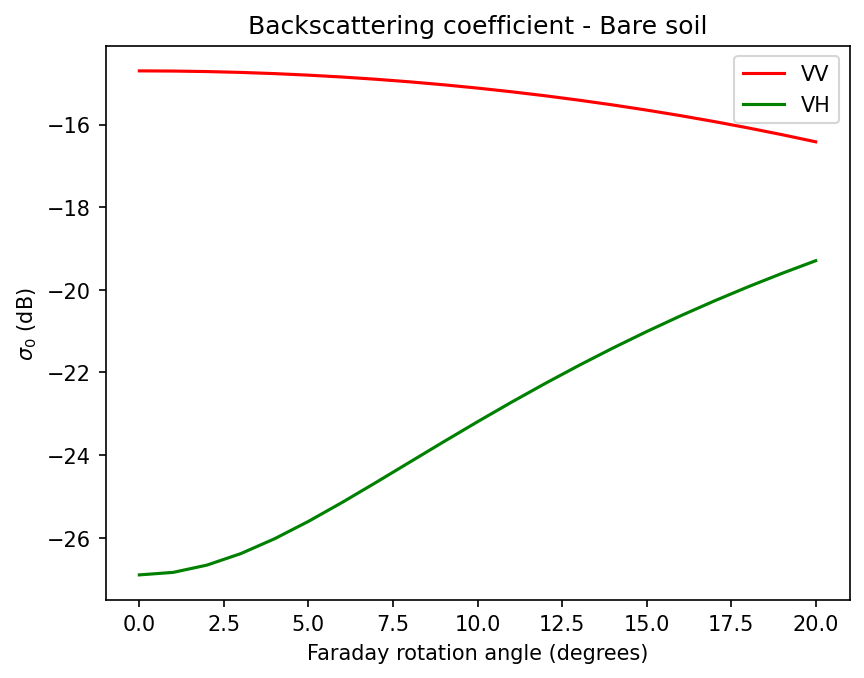
\includegraphics[width=0.32\textwidth]{Figures/pol/FR_bacskcatter_Bare soil.png}
 & 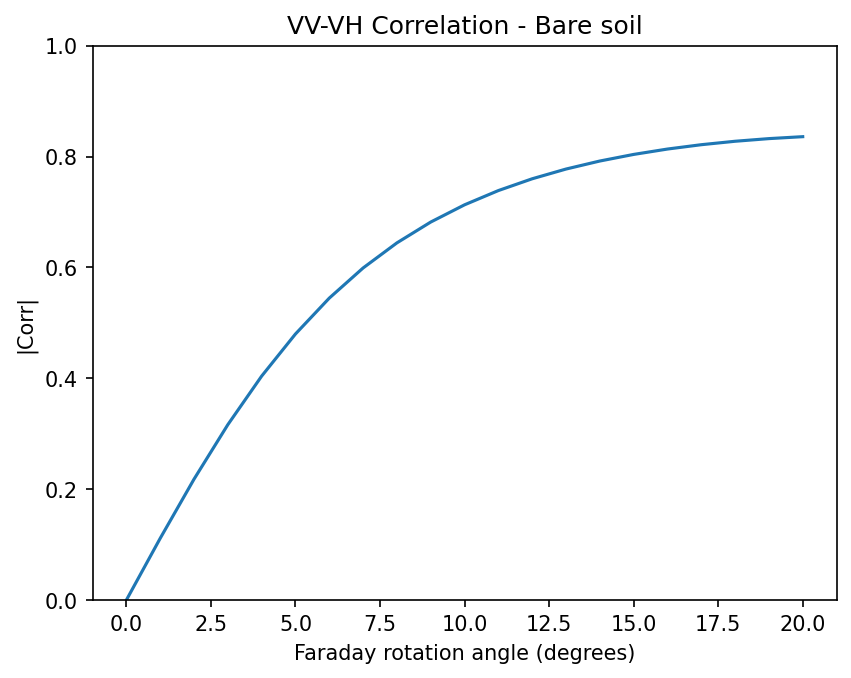
\includegraphics[width=0.32\textwidth]{Figures/pol/FR_VV-VH_Correlation_Bare soil.png}
 &
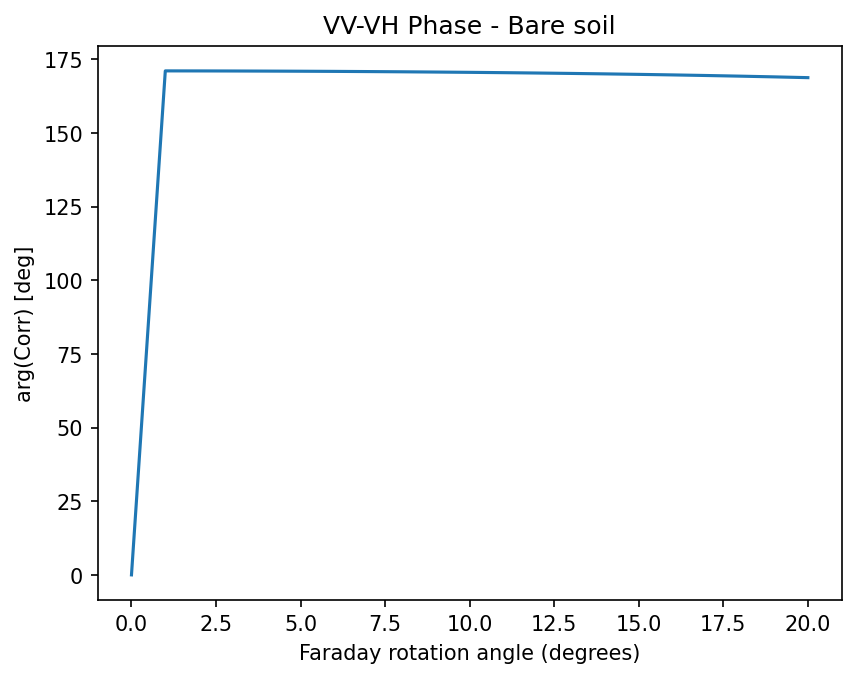
\includegraphics[width=0.32\textwidth]{Figures/pol/FR_VV-VH_Phase_Bare soil.png} \\
(a) & (b) &
(c) 
\end{tabular}
\caption{Effect of \acs{fr} upon the dual-pol response of bare soil. (a) Backscattering coefficients, (b) Correlation between channels, (c) Phase between channels.}
\label{fig:pol_fr_dualpol_baresoil}
\end{figure}
\begin{figure}[h!]
\centering
\begin{tabular}{ccc}
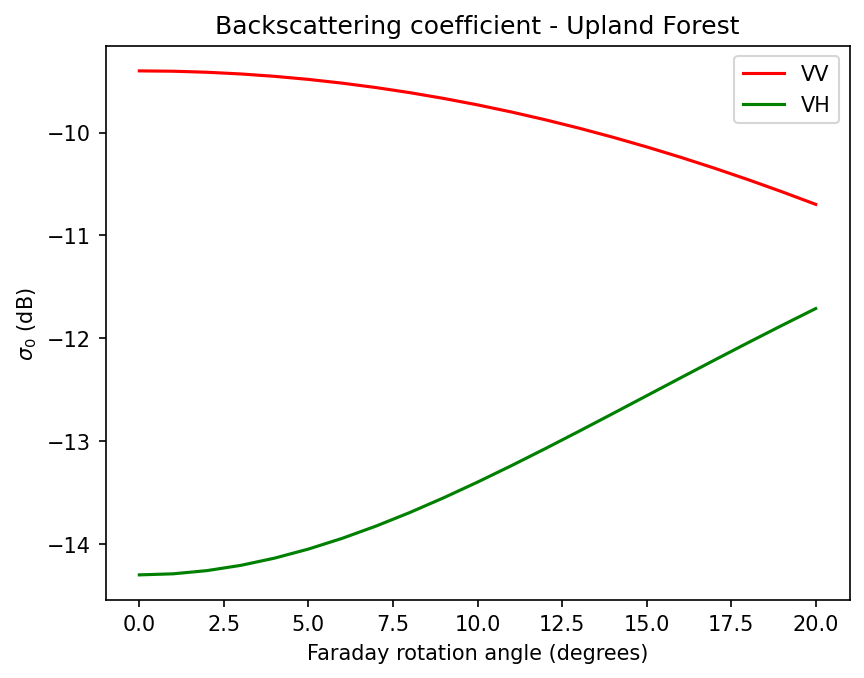
\includegraphics[width=0.32\textwidth]{Figures/pol/FR_bacskcatter_Upland Forest.png}
 & 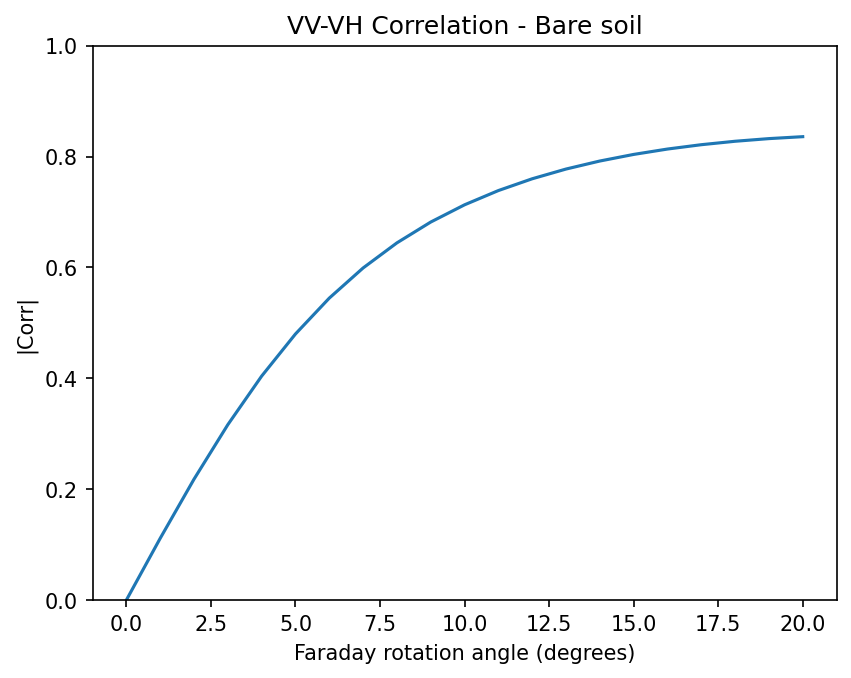
\includegraphics[width=0.32\textwidth]{Figures/pol/FR_VV-VH_Correlation_Bare soil.png}
 &
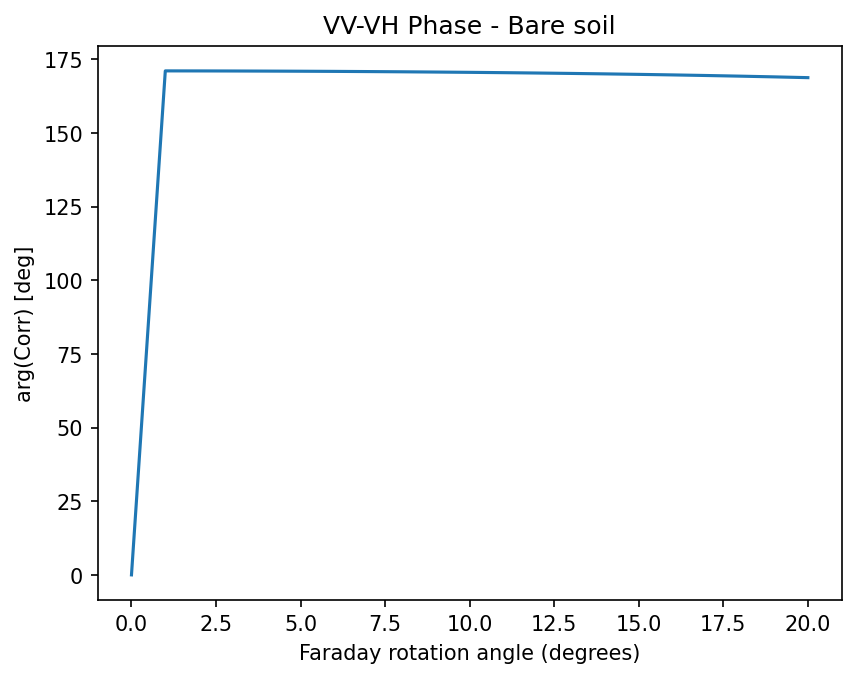
\includegraphics[width=0.32\textwidth]{Figures/pol/FR_VV-VH_Phase_Bare soil.png} \\
(a) & (b) &
(c) 
\end{tabular}
\caption{Effect of \acs{fr} upon the dual-pol response of forest. (a) Backscattering coefficients, (b) Correlation between channels, (c) Phase between channels.}
\label{fig:pol_fr_dualpol_forest}
\end{figure}

The backscattering coefficient at the copolar channel (VV) decreases as the rotation angle increases. This decrease is almost negligible for angles lower than 5~degrees, and reaches 1 to 2~dB at the extreme cases (rotation angle equal to 20~degrees). At the cross-polar channel (VH), the backscattering coefficient increases proportionally to the \acs{fr} angle, reaching a bias of 7~dB for bare soil (\autoref{fig:pol_fr_dualpol_baresoil}a) and 3~dB for forest (\autoref{fig:pol_fr_dualpol_forest}a). 

Due to the cross-talk induced by \acs{fr}, the most severely affected polarimetric variable is the correlation between channels. A scene characterised by null correlation exhibits a rapidly increasing correlation as a consequence of \acs{fr}. For instance, it reaches 0.5 at a rotation angle of 5~degrees, and saturates at around 0.8 for rotation angles above 15~degrees.

The phase difference between the two channels is not defined when the correlation between channels is null. However, it takes a value close to 180~degrees as soon as the  \acs{fr} make the correlation depart from zero.

In the same vein, Figure 3 shows the false colour RGB composites of a SAOCOM scene over Naples when \acs{fr} is injected into the data and no correction is applied. For this purpose, the backscattering level of HH is assumed equal to VV and the correlation between HH and VV is assumed to be 0.5 with zero phase. This has been applied as a constant for the whole scene, but these values could be changed in a more sophisticated way, e.g. as a function of the land cover type.

\begin{figure}[ht!]
\centering
\begin{tabular}{cc}
No FR & 5 degrees \\
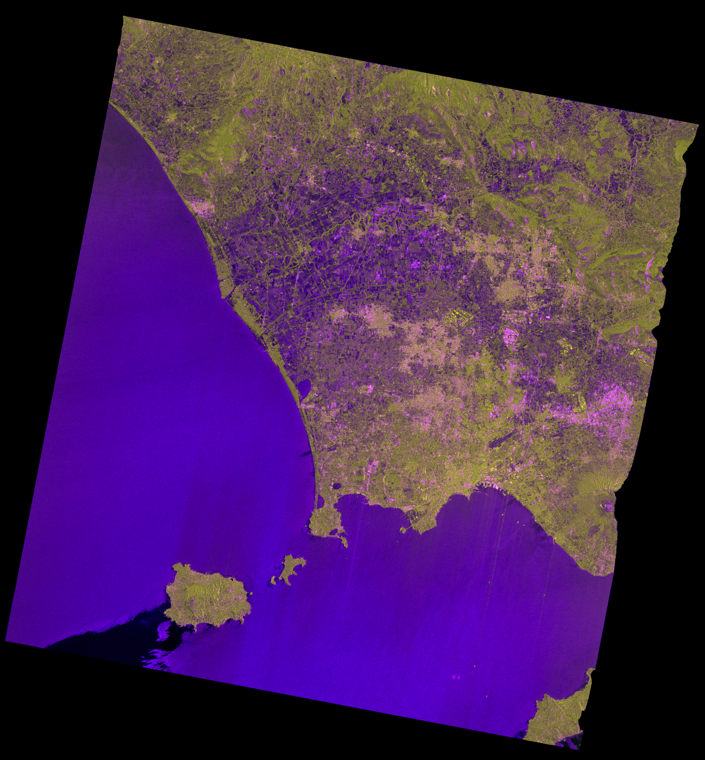
\includegraphics[width=0.45\textwidth]{Figures/pol/SAOCOM_RGB_noFR.png}
 & 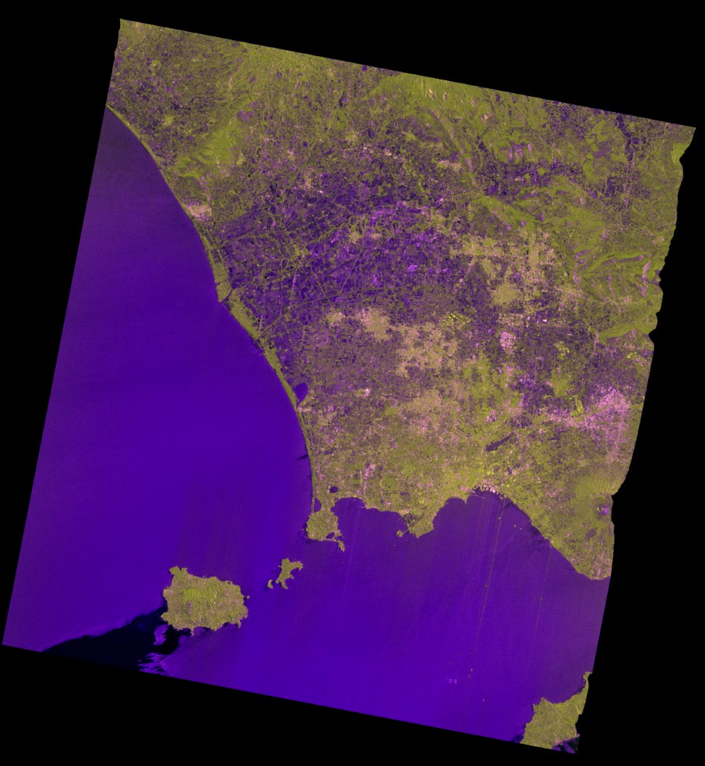
\includegraphics[width=0.45\textwidth]{Figures/pol/SAOCOM_RGB_FR_5deg.png}
 \\
10 degrees & 20 degrees \\
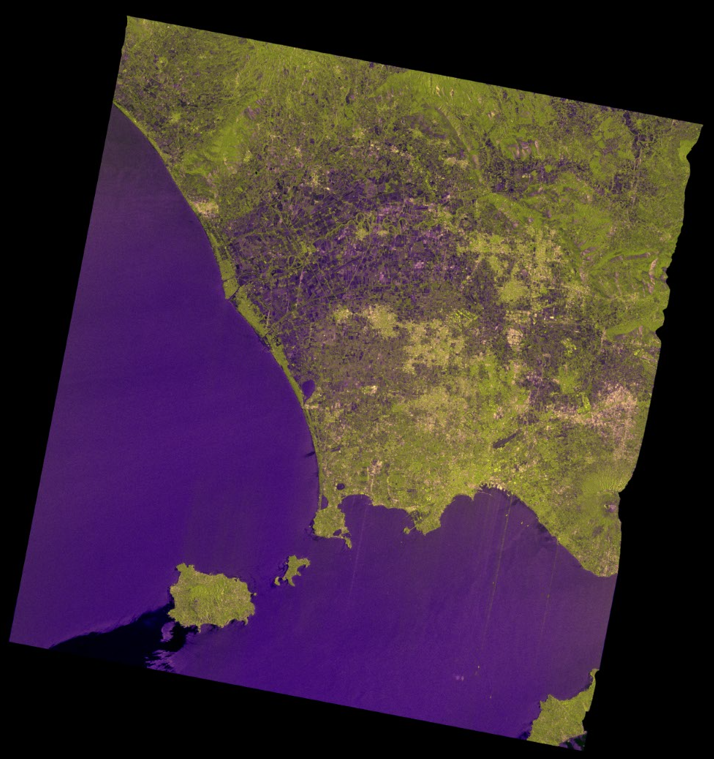
\includegraphics[width=0.45\textwidth]{Figures/pol/SAOCOM_RGB_FR_10deg.png}
 & 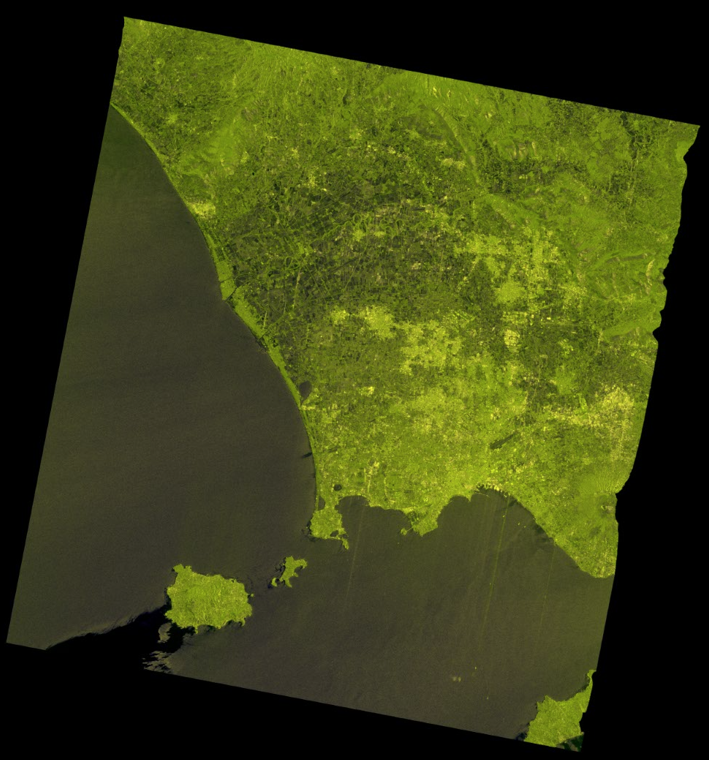
\includegraphics[width=0.45\textwidth]{Figures/pol/SAOCOM_RGB_FR_20deg.png}

\end{tabular}
\caption{RGB false colour composite of a SAOCOM dual-pol image over Naples (DSC/S4). Channels: R: VV, G: VH: B: VV/VH. The original image (top left) is compared with other three cases in which different \acs{fr} angles were injected (5, 10 and 20~degrees). The backscattering level of HH is assumed equal to VV and the correlation between HH and VV is assumed to be 0.5 with zero phase, and both are assumed constant over the whole scene.}
\label{fig:pol_FR_RGB}
\end{figure}

The visual aspect of the RGB composite when the \acs{fr} angle  is 5~degrees is very similar to the case without \acs{fr}, as the VV backscattering coefficient is almost unaltered and the VH one is only increased by less than 2~dB. A \acs{fr} angle of 10~degrees is more noticeable in this image: the sea becomes purple instead of blue, and all areas originally represented in pink colour (corresponding to buildings and urban land cover) become yellowish. In the most extreme case (\acs{fr} angle equal to 20~degrees) the polarimetric information is lost, and the resulting image is all shown in the same green hue, with its brightness defined by the span (backscactered power).

A summary of the results of a simple correction approach for dual-pol data, using real measurements of \acs{tec}, and the expected impact of \acs{fr} FR for ROSE-L were described in Chapter~6 of \citep{Hajnsek2019}.
Assuming certain knowledge on the scene (land cover and scattering properties), which can be obtained from other quad-pol L-band images of other sensors (e.g. ALOS-PALSAR and NISAR), and by using an external measure of \acs{tec}, it is possible to approximately correct the effect of FR on dual-pol data. These approaches  could be readily implemented, and they could be tested using quad-pol data as a reference. If no correction is applied, external \acs{tec} values could be used to estimate the \acs{fr} rotation angle and produce an auxiliary map with the expected impact of \acs{fr} (or a mask map if binarized). 



\section{Ocean Radar Backscatter (ORB)}
\label{sec:orb}
The ORB product is relatively straightforward to derived from the NRB product. Therefore, most of the critical processing steps have been addressed during NRB product generation. In addition to the NRB input, the generate of the ORB products requires ERA5 wind data and geophysical model functions (GMF). The ORB product includes multiple layers of $\sigma_{0}$ values, each corresponding to a specific processing stage: a full-resolution outlier mask in $\sigma_{0}$ convention, spatially averaged noise-equivalent $\sigma_{0}$, denoised $\sigma_{0}$, denoised and outlier-removed $\sigma_{0}$, and angle-of-incidence compensated $\sigma_{0}$.
\subsection{Evaluation criteria}
\label{sec:orb_criteria}
The main layer of the ORB products are the spatially-averaged, denoised, and outlier-removed $\sigma_{0}$, and the angle-of-incidence-compensated $\sigma_{0}$. The quality of the former is assessed through statistical analysis of the product itself, whereas the latter is evaluated through inter-comparison of results derived from Sentinel-1 C-band and SAOCOM L-band observations.

Using an example from SAOCOM observations, the performance of the outlier removal processing is summarized in Table \ref{tab:stats_sigma0}, which presents the statistics of the raw $\sigma_{0}$, identified outliers $\sigma_{0}$, and the resulting outlier-free $\sigma_{0}$.
\begin{longtblr}[
	label = tab:stats_sigma0,
	entry = none,
	caption = {Statistics of different layer of $\sigma_{0}$},
	]{
		width = \linewidth,
		colspec = {Q[l,20]Q[c,20]Q[c,20]Q[c,20]},
		hlines,
		hline{1-Z} = {-}{0.05em},
	}
	\textbf{Statistics}   & \textbf{$\sigma_{0,\mathrm{raw}}$}   & \textbf{$\sigma_{0,\mathrm{outlier}}$} & \textbf{$\sigma_{0,\mathrm{L}}$} \\
	Mean & 0.06 & 0.67 & 0.06 \\
    Median & 0.04 & 0.33 & 0.04 \\
    Standard deviation & 0.50 & 4.34 & 0.23 \\
\end{longtblr}
According to the statistics, the mean and median of the $\sigma_{0}$ values are preserved after the outlier removal, while the standard deviation is reduced by approximately $50\%$.

A comparison of Sentinel-1 and SAOCOM results is illustrated in Figure \ref{fig:orb_sentinel_saocom}.
\begin{figure}[ht!]
\centering
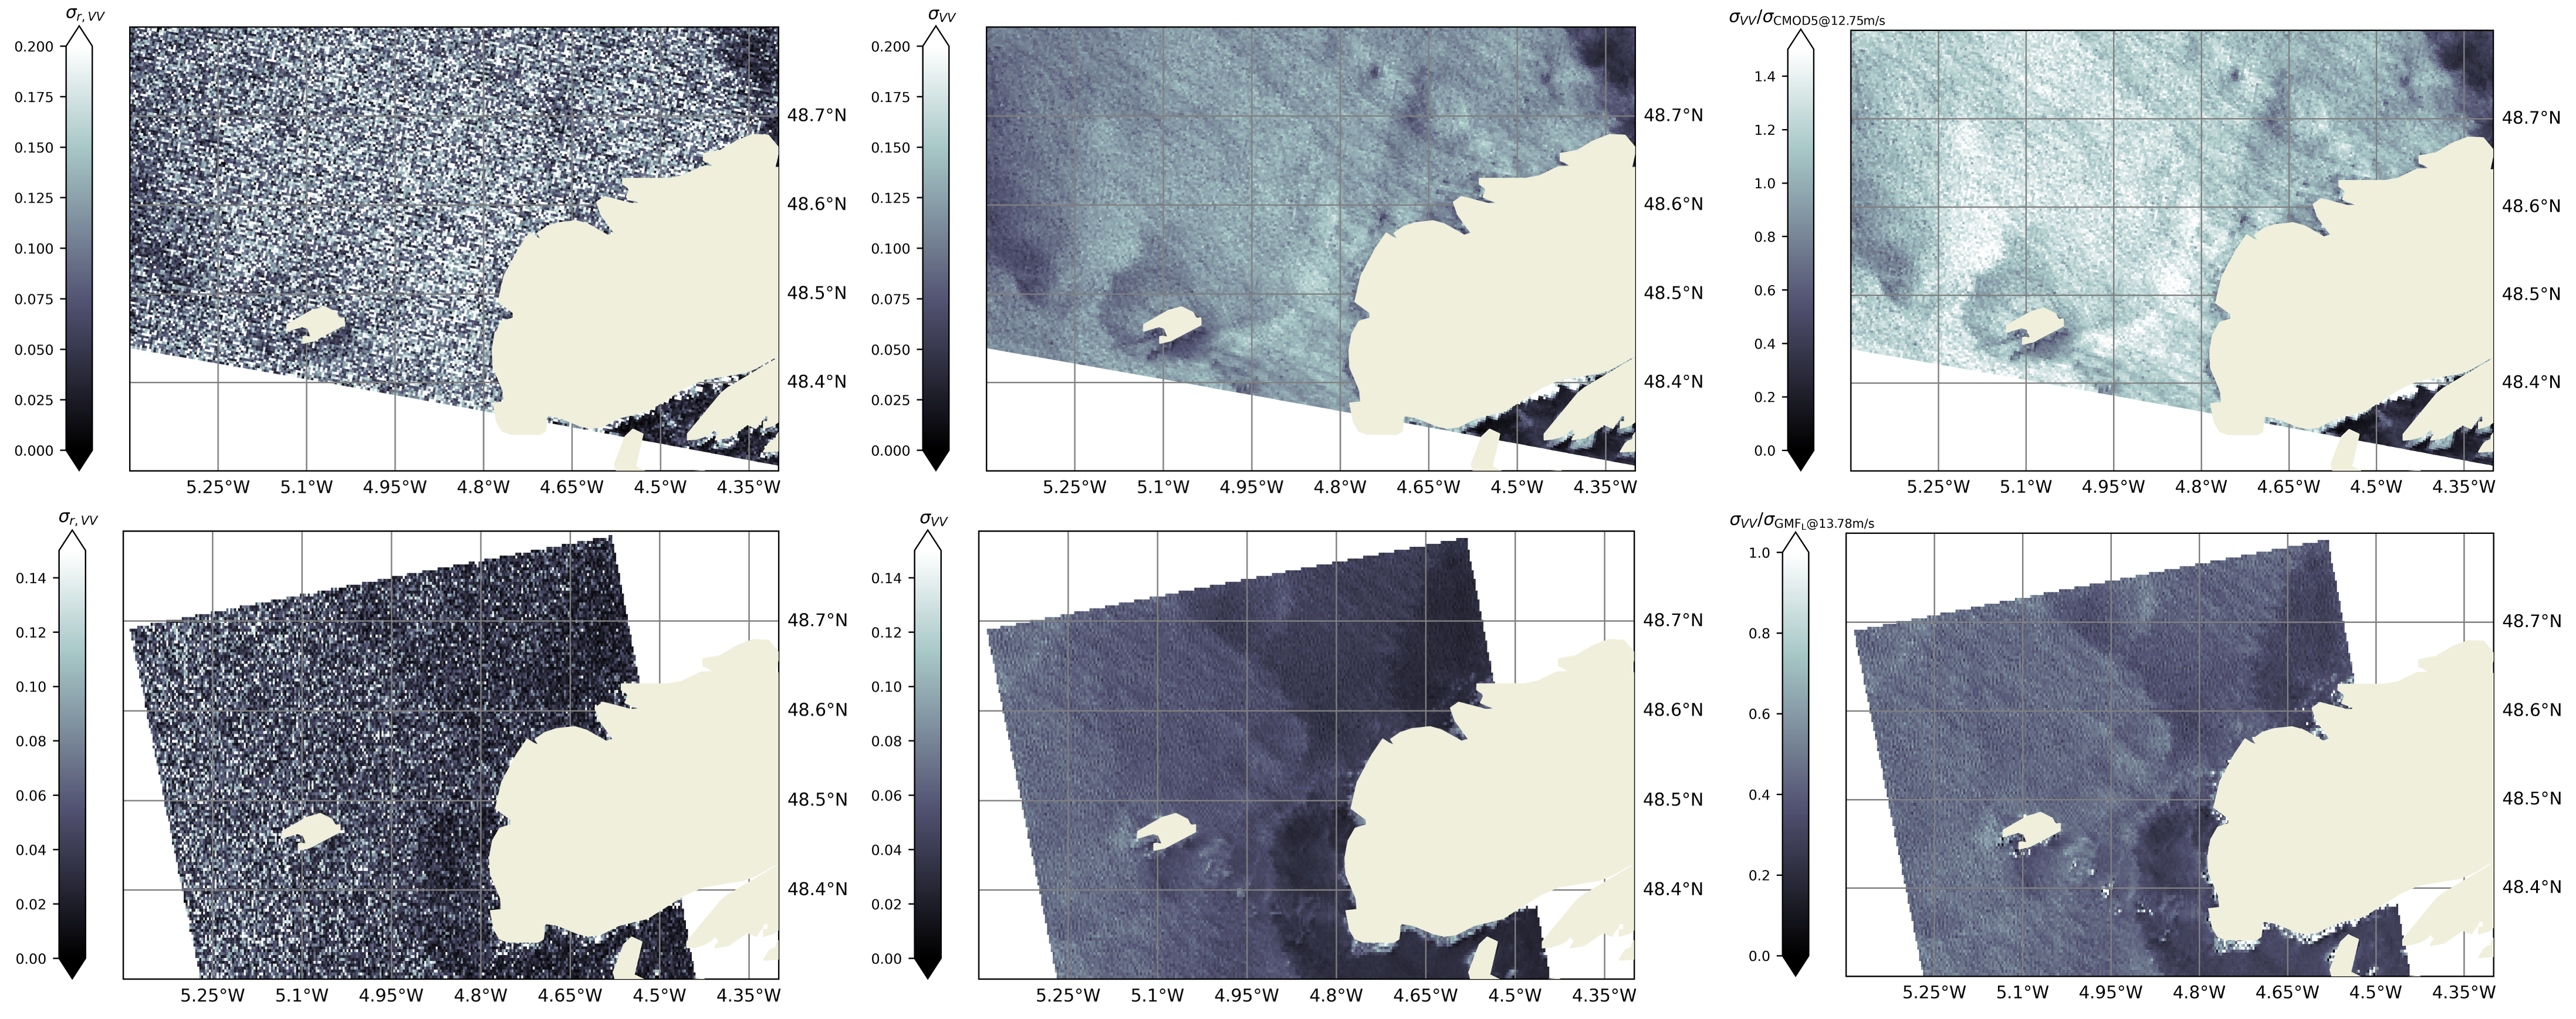
\includegraphics[width=0.9\textwidth]{Figures/oceans/D5_sentinel_saocom.png}
\caption{ORB products comparison between Sentinel-1 (upper panel) and SAOCOM (lower panel).From left to right are raw $\sigma_{0}$, denoised and outlier-free $\sigma_0$, and the angle of incidence compensated $\sigma_{0}$.}
\label{fig:orb_sentinel_saocom}
\end{figure}
Both observations were acquired on the same date, 2023-11-03, with the SAOCOM acquisition at 06:00:43 occurring approximately half an hour earlier than the Sentinel-1 acquisition at 06:32:31. Despite differences in acquisition mode, geometry and frequency, and the highly dynamic nature of the ocean, the roughness values in the ORB products exhibit comparable magnitudes.
\subsection{Theoretical models}
\label{sec:orb_models}
The processing of ORB products involves two essential steps: bright target removal and angle-of-incidence compensation, both of which incorporate theoretical models.
\subsubsection{Bright target removal}
To identify the bright target statistically, the sigma0 is low-pass filtered with a Gaussian window
\begin{equation}
    I^{\mathrm{LPF}}(x,y) = I(x,y)*h_{\mathrm{LP}}(x,y),
\end{equation}
with
\begin{equation}
    h_{\mathrm{LP}}(x,y) = \frac{1}{\sigma_x\sigma_y\sqrt{2\pi}}e^{-\frac{x_{i}^{2}}{2\sigma_{x}^{2}}-\frac{y_{i}^{2}}{2\sigma_{y}^{2}}},
\end{equation}
the impulse reponse of the Gaussian filter, where $\sigma_{x,y}$ are the filter widths, which can be in the order of km. We then compute the intensity contrast as
\begin{equation}
    K(x,y) = \frac{I(x,y) - I^{\mathrm{LPF}}(x,y)}{I^{\mathrm{LPF}}(x,y)}.
\end{equation}
Pixels for which the intensity contrast exceeds a given threshold,
\begin{equation}
    K(x,y) >K_{\mathrm{thres}}
\end{equation}
are considered outliers. Consequently, a mask is generated according to 
\begin{equation}
    M(x,y) = \begin{cases}
    1, & \text{if } K(x,y) < K_{\mathrm{thres}} \\
    0,  & \text{if } K(x,y) > K_{\mathrm{thres}}
    \end{cases}.
\end{equation}

To define the contrast threshold, we assume the intensity distribution of a single-look pixel is exponential, then the mean and standard deviation of the intensity are equal to $\frac{1}{\lambda}$. The summation of multiple independent exponential distributions changes the statistics. According to error propagation law, the mean and the standard deviation is scaled with the number of independent samples, in this case, the equivalent number of looks (ENL). The mean and the standard deviation are
\begin{equation}
    \mu = \frac{\mathrm{ENL}}{\lambda}, \sigma = \frac{\sqrt{\mathrm{ENL}}}{\lambda}.
\end{equation}
Therefore, the standard deviation can be written as a scaled mean
\begin{equation}
    \sigma = \frac{\mu}{\sqrt{\mathrm{ENL}}}.
\end{equation}
After the outlier removal, the energy loss due to the mask is restored. This is done by dividing the masked $\sigma_0$ by the low-pass filtered mask. Then, the noise-floor is subtracted. 
\begin{equation}
    \sigma_{0,\mathrm{L}} = \frac{(I(x,y)\cdot M(x,y))*h_{\mathrm{LP}}(x,y)}{M(x,y)*h_{\mathrm{LP}}(x,y)}-\mathrm{NESZ}.
\end{equation}
After these steps, the downsample is performed by using the resolution of the input data and the user desired resolution as input parameters.
\subsubsection{Angle of incidence compensation}
This step involves feeding a GMF with ERA5 wind products and the SAR imaging geometry. The angle-of-incidence compensation is then performed by scaling the downsampled product using the ratio $\sigma_{0,\mathrm{L}} / \sigma_{0,\mathrm{mod}}$, where $\sigma_{0,\mathrm{L}}$ is the locally observed backscatter and $\sigma_{0,\mathrm{mod}}$ is the GMF-predicted backscatter. The GMF for NRCS over ocean is generally expressed as:
\begin{equation}
    \sigma_{0,\mathrm{mod}}  = A_0(w,\theta)(1 + A_1(w,\theta)\cos{\varphi}+A_2(w,\theta)\cos{2\varphi}),
\end{equation}
where $\varphi$ is the relative wind direction with respect to the radar, $A_n(w,\theta)(n=0,1,2)$ is a function of wind speed $w$ and the incident angle $\theta$. For modeling NRCS from co-polarized L-band acquisitions, the definition of each $A$ function follows \cite{isoguchi_l-band_2009}, while for C-band, the forward CMOD5.N model is used.
\subsection{Computational performance}
\label{sec:orb_computation}
The computational load of generating the ORB product is comparable to that of the NRB product, although the ORB product includes more layers. The most computationally expensive step is the 2D Gaussian blurring, which is applied three times during the outlier removal process. For a single image, the total processing time of generating ORB from NRB is approximately $12.7$ seconds.
\subsection{Criticalities and weakness}
\label{sec:orb_criticalities}
Any quality assessment of the ORB product depends on the quality of the input NRB data, wind data, and geophysical model function (GMF), rather than the ORB algorithm itself. It remains unclear whether a local or global mean wind reference is more suitable for roughness computation, as each approach has its own advantages and limitations. At present, we use the local mean wind as a reference, as it provides better compensation for the angle of incidence dependence. 

\section{Precise Range \ Azimuth Offsets (PRO / PAO \& GPRO / GPAO )}
\label{sec:pro_pao}

\subsection{Evaluation criteria}
\label{sec:pro_pao_criteria}

The pixel offset products provide measurements of local displacements in the range and azimuth directions between a reference and a secondary \acs{cslc}, forming a \acs{cslc} pair. These offsets can be estimated using either phase or amplitude information.

Phase information enables the retrieval of both slant range and azimuth offsets in regions where two distinct looks of the same scene are available. For Sentinel-1 data, this is only feasible within the limited areas of burst overlap, due to the specific geometry of the TOPSAR acquisition mode. Nevertheless, the phase modulation inherent to TOPSAR improves measurement sensitivity, provided that interferometric phase continuity is maintained across adjacent bursts. The residual phase, after conventional processing, can also be exploited to identify motion components in the azimuth direction, offering valuable insight into dynamic surface processes such as glacier flow or landslides. When applicable, phase-based techniques are preferred due to their superior accuracy, which is a consequence of the high sensitivity of the interferometric phase to small displacements.

In cases where phase information is unavailable, decorrelated, or when the displacement to be measured is particularly large (such that phase measurements may underestimate its magnitude due to phase wrapping), amplitude-based methods are employed. These rely on normalized cross-correlation between image patches to estimate local shifts in both range and azimuth directions. Although typically less precise, amplitude-based methods offer broader applicability over heterogeneous surfaces and in low-coherence areas.

The accuracy of the \acs{pro} / \acs{pao} products is critically influenced by the chosen estimation technique, the sensor characteristics, and the properties of the observed scene. For the purpose of this analysis, we assume that ionospheric effects—particularly dispersive phase distortions and group delay—have been properly compensated, either through external ionospheric correction data or via differential techniques that inherently mitigate such disturbances. Indeed, if not correctly addressed, these effects can be erroneously interpreted as surface displacements.

Under this assumption, the remaining sources of error primarily arise from thermal noise, spatial decorrelation, terrain-induced geometric distortions, and limitations of the processing algorithms. These factors affect the precision and reliability of the derived displacement measurements and must be considered in the quality assessment.

To evaluate the achievable accuracy of the \acs{pro} / \acs{pao} products, we analyze the two proposed approaches to estimate range and azimuth shifts (phase-and amplitude-based). In the following, we provide a theoretical examination of the expected quality associated with each method, focusing on their sensitivity and applicability.

\subsection{Theoretical models}
\label{sec:pro_pao_models}

Two methods are proposed for the estimation of pixel offsets in SAR data: phase-based and amplitude-based techniques. Each method is grounded in a distinct theoretical model and is characterized by specific assumptions, performance expectations, and error sources.

\paragraph{Phase-based estimation}

Phase-based methods rely on the coherent phase difference between two complex, co-registered \acs{sar} images (\acs{cslc}). In regions with sufficient coherence $\gamma$, the interferometric phase $\phi$ can be used to retrieve fine displacement information in the range direction, and—under certain constraints—also in the azimuth direction.

For simplicity, we consider two co-registered \acs{sar} images (\acs{cslc}): a reference image $R$ and a slave image $S$. The displacement in the slant range direction, $dr$, corresponding to an area of \(X \times Y\) pixels centered at radar coordinates \((\mathrm{rg}, \mathrm{az})\), can be computed by converting the unwrapped interferometric phase $\phi$ using:

\begin{equation}
dr = \frac{\lambda}{4\pi} \phi
\label{eq:dr_to_phi}
\end{equation}

where $\lambda$ is the radar wavelength, and $\phi$ is the multilooked (i.e., spatially averaged) version of the interferometric phase over the selected window. This formulation assumes that the phase is unambiguous (i.e., properly unwrapped), that atmospheric and ionospheric contributions have been either corrected or strongly mitigated, and, when possible, that the interferogram has been corrected for azimuth displacements.

Evaluating the accuracy of the estimated slant range displacement thus corresponds to assessing the accuracy of the unwrapped interferometric phase. Ignoring unwrapping errors—which, when present, can significantly degrade measurement quality (see Section~\ref{sec:pro_pao_criticalities})—the theoretical accuracy is bounded by the Cramér–Rao lower bound for phase estimation. The standard deviation of the averaged interferometric phase is given by:

\begin{equation}
\sigma_{\phi} = \frac{1}{\sqrt{N}} \cdot \frac{\sqrt{1 - |\gamma|^2}}{|\gamma|}
\label{eq:sigma_phi}
\end{equation}

where $|\gamma|$ is the coherence computed in the \(X \times Y\) window and $N$ is the number of pixels within this window (i.e. $N=X Y$.

The corresponding standard deviation of the estimated slant range displacement is then:

\begin{equation}
\sigma_{dr} = \frac{\lambda}{4\pi} \cdot \frac{1}{\sqrt{N}} \cdot \frac{\sqrt{1 - |\gamma|^2}}{|\gamma|}
\label{eq:sigma_dr}
\end{equation}

This expression highlights that the accuracy of phase-based offset estimation improves with higher coherence and larger averaging windows.

The phase-based technique we propose for estimating the shift in the azimuth direction was originally developed to improve the co-registration of a slave image with respect to its master \cite{Scheiber2000, Prats2012}. It has been extensively demonstrated that this approach enables the reliable detection of subtle motion in the azimuth direction.

To apply this technique, two-look imaging over the same area is required—that is, two nearly simultaneous acquisitions of the same scene with sufficient Doppler centroid separation. The greater the Doppler separation, the higher the sensitivity to azimuthal motion. This condition is particularly well satisfied in Sentinel-1 TOPS mode, where azimuth beam steering introduces significant squint angle diversity within the overlap regions of consecutive bursts. As a result, in the case of Sentinel-1 TOPS mode data, this method provides enhanced sensitivity to azimuthal motion compared to conventional split-beam interferometry, typically applied to Stripmap or ScanSAR acquisitions. A limitation of this approach when applied to Sentinel-1 TOPS mode, however, is that it can only be used in burst overlap regions, which do not cover the entire scene. 

As in the previously discussed case of slant range motion estimation via phase, we now consider two co-registered \acs{sar} images (\acs{cslc}): a reference image $R$ and a slave image $S$. We focus on those regions of the scene where we have two looks with sufficient Doppler separation—namely, the overlap areas between consecutive bursts in Sentinel-1 TOPS acquisitions. For each tile within these regions, consisting of \(X \times Y\) pixels and centered at radar coordinates \((\mathrm{rg}, \mathrm{az})\), we compute the average of the phase difference $\psi$ derived from the two available interferograms as:

\begin{equation}
\psi = \arg\left\{R_{A} \cdot S_{A}^{*} \cdot R_{B} \cdot S_{B}^{*}\right\}
\label{eq:psi}
\end{equation}

Here, $A$ and $B$ identify the two observations with sufficient Doppler separation (in the Sentinel-1 case, these correspond to two consecutive bursts within the same sub-swath). From the phase difference $\psi$, the azimuth displacement $da$ (in meters) can be computed using the relation (\cite{Scheiber1999}):

\begin{equation}
da = \frac{v_{g}}{2\pi \Delta f_{d}} \psi
\label{eq:da_from_psi}
\end{equation}

where $v_{g}$ is the satellite velocity and $\Delta f_{d}$ is the Doppler centroid separation between the two looks. Since $da$ is linearly proportional to the phase difference $\psi$, evaluating the accuracy of the azimuth displacement estimate corresponds to assessing the precision of this phase measurement. Applying the Cramér–Rao lower bound for phase estimation, the standard deviation of the azimuth displacement can be expressed as:

\begin{equation}
\sigma_{da} = \frac{v_{g}}{2\pi \Delta f_{d}} \cdot \frac{1}{\sqrt{N}} \cdot \frac{\sqrt{1 - |\gamma|^2}}{|\gamma|}
\label{eq:sigma_da}
\end{equation}

where $N = X \times Y$ is the number of independent samples used in the averaging, and $|\gamma|$ is the coherence within the tile. 

The following figures graphically illustrate how the accuracy in estimating displacement in both the slant-range and azimuth directions—using the previously described phase-based method—depends on the coherence value ($\gamma$) and the number of pixels N used in the averaging process. Specifically, the first pair of images shows the slant-range accuracy achievable with this method.

In Figure~\ref{fig:rg_accuracy_phase}, the accuracy for displacement estimation in the slant-range direction is presented. The left plot shows the expected accuracy when using \acs{s1} data, while the right plot shows the corresponding accuracy using \acs{rosel} data.

In each plot, the colored curves represent different values of N (i.e., the number of pixels used in the average). It is clearly visible that, for fixed values of N and $\gamma$, the expected accuracy with \acs{s1} is significantly better. This is due to the fact that \acs{s1} operates at a wavelength that is four times shorter than \acs{rosel}'s, resulting in a higher sensitivity to displacement in the slant-range direction.

\begin{figure}[ht!]
\centering
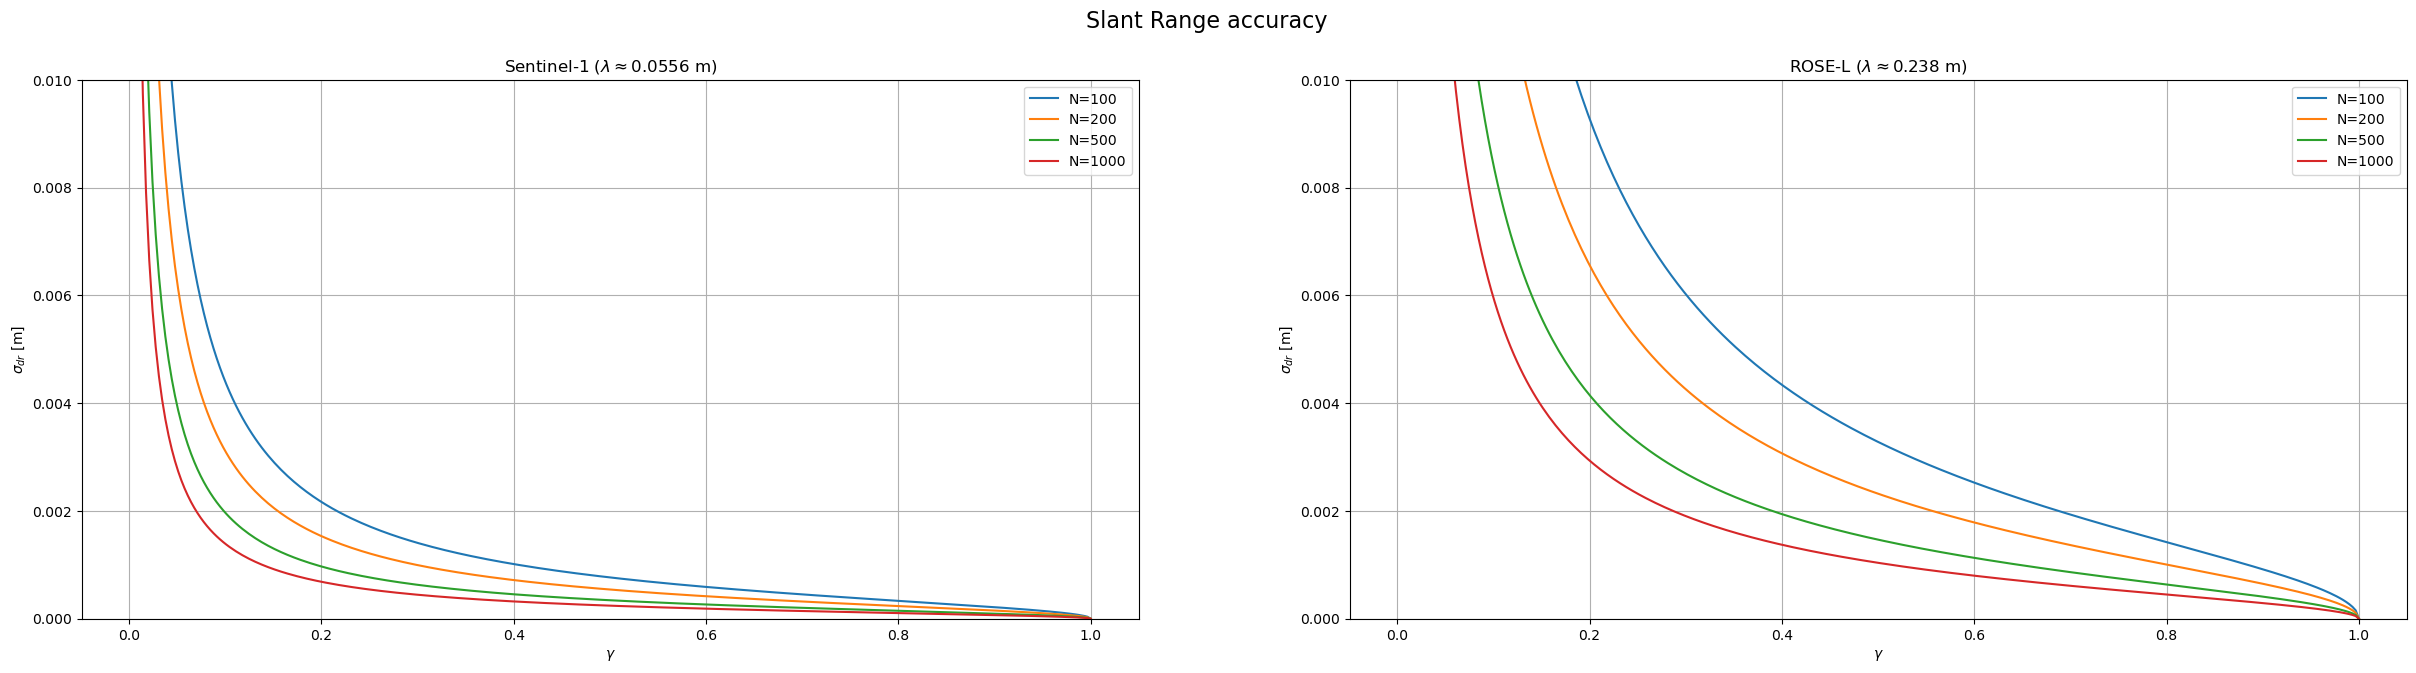
\includegraphics[width=0.9\textwidth]{Figures/pro_pau/rg_accuracy_ph_method.png}
\caption{Slant-range displacement accuracy as a function of coherence ($\gamma$) and the number of pixels N used for averaging, obtained using the phase-based method. The left plot shows results for Sentinel-1, while the right plot shows those for \acs{rosel}. Each colored curve corresponds to a different value of N. Due to its shorter wavelength, Sentinel-1 provides higher sensitivity to displacement, resulting in better accuracy for the same $\gamma$ and N values.}
\label{fig:rg_accuracy_phase}
\end{figure}

Figure~\ref{fig:az_accuracy_phase} illustrates the achievable accuracies in the azimuth direction using the phase-based estimation method, applied to \acs{s1} data (left panel) and \acs{rosel} data (right panel). The curves are plotted as a function of coherence \(|\gamma|\), with different colors corresponding to different values of \(N\), i.e., the number of pixels used in the averaging window. Due to the significantly larger Doppler centroid separation in the burst overlap regions of \acs{s1} acquisitions, the resulting sensitivity to azimuthal motion is notably higher than expected for \acs{rosel}. Consequently, for the same values of \(N\) and coherence, the \acs{s1} case yields substantially better accuracy in azimuth displacement estimation.

\begin{figure}[ht!]
\centering
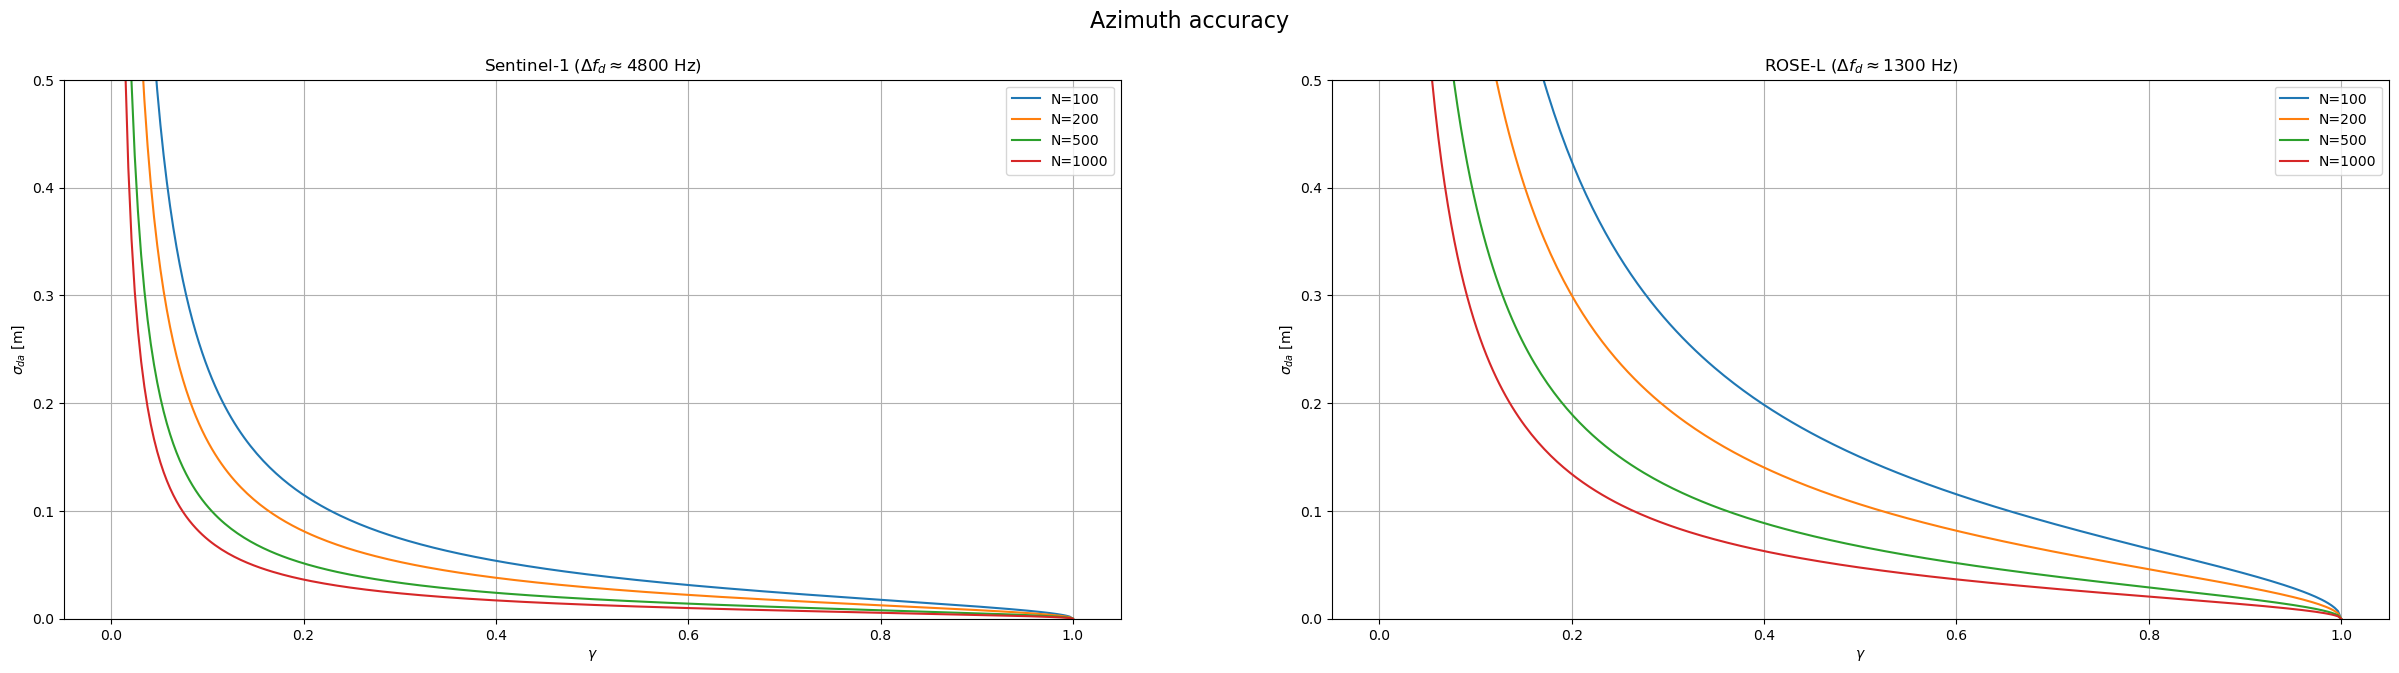
\includegraphics[width=0.9\textwidth]{Figures/pro_pau/az_accuracy_ph_method.png}
\caption{Estimated azimuth displacement accuracy as a function of coherence for different values of \(N\) (number of pixels used in phase averaging), using the phase-based method. Results are shown for \acs{s1} data (left) and \acs{rosel} data (right). The improved Doppler centroid separation in \acs{s1} burst overlaps leads to significantly higher sensitivity to azimuthal motion compared to \acs{rosel}, resulting in lower displacement uncertainty for the same averaging window size and coherence.}
\label{fig:az_accuracy_phase}
\end{figure}

In the following Figure~\ref{fig:example_azimuth_shift_phase} we present some experimental results obtained using \acs{s1} data. As the standard \acs{s1} \acs{slc} products typically provide only a few tens of pixels of overlap between consecutive bursts, and since the phase-based azimuth offset estimation method is only applicable within these overlap regions, we used a custom reprocessed dataset over Greenland. This dataset was specifically modified to increase the overlap between bursts to more than three hundred pixels.

Starting from \acs{cslc} products, we generated an interferogram without applying any Enhanced Spectral Diversity (\acs{esd}) procedure. The phase component corresponding to the displacement in the azimuth direction (as defined by Equation~\ref{eq:psi}) was estimated within the burst overlap regions. Figure~\ref{fig:example_azimuth_shift_phase} shows the interferogram, obtained by mosaicking three consecutive bursts and applying a multilooking factor of 12 (slant range) by 4 (azimuth), along with the phase signal which, when unwrapped and converted to meters, corresponds directly to the azimuth displacement.

This simple experiment demonstrates the applicability of the proposed phase-based approach, as the phase retrieved in the overlap areas shows a coherent pattern. It is not dominated by noise; rather, it clearly contains measurable signal information. At the same time, the bottom panel of Figure~\ref{fig:example_azimuth_shift_phase} highlights one of the primary challenges associated with this method: the requirement for two observations of the same scene with sufficient Doppler separation.

\begin{figure}[ht!]
\centering
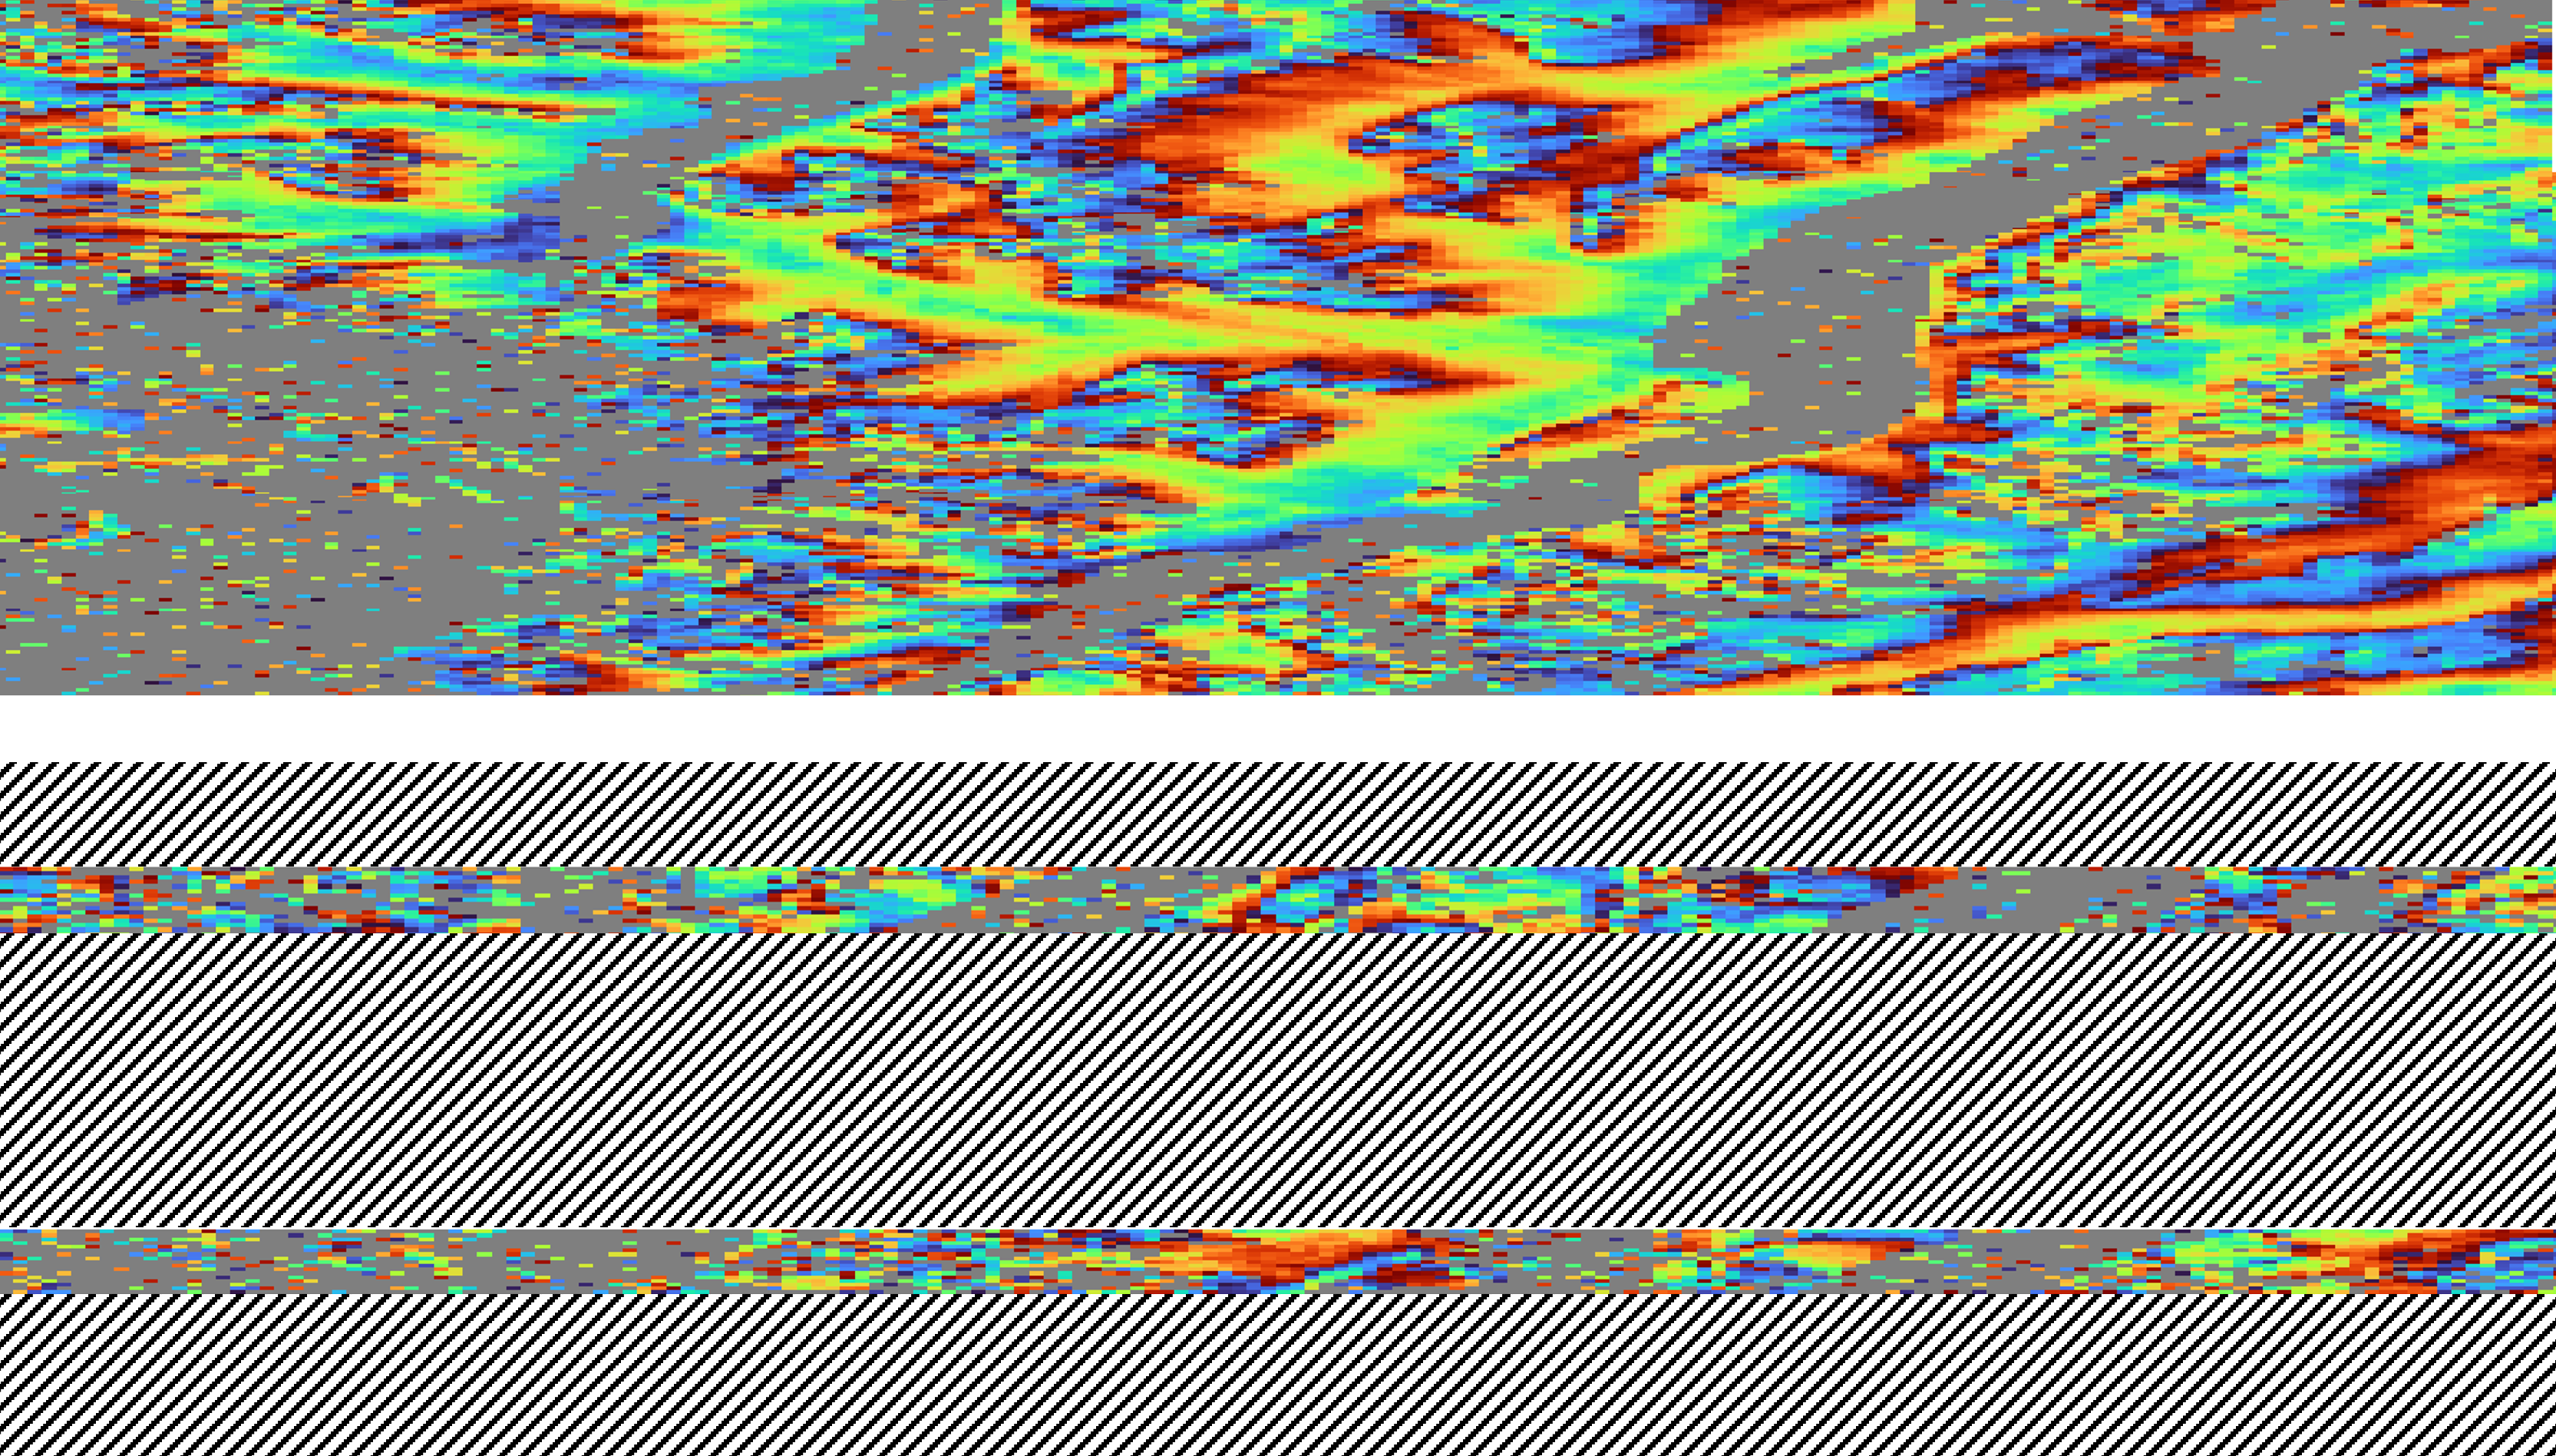
\includegraphics[width=0.9\textwidth]{Figures/pro_pau/example_azimuth_shift_phase.png}
\caption{Top: interferogram obtained by mosaicking three consecutive bursts and applying a multilooking factor of 12 in slant range and 4 in azimuth. The displayed phase component corresponds to the azimuth displacement, which can be unwrapped and converted to meters using Equation~\ref{eq:da_from_psi}. Bottom: estimated azimuth displacement shown only within the burst overlap regions, where phase-based estimation is feasible due to sufficient Doppler separation. Oblique blank areas indicate regions with no burst overlap, where azimuthal shifts cannot be retrieved using this method.}
\label{fig:example_azimuth_shift_phase}
\end{figure}


\paragraph{Amplitude-based estimation using Incoherent Cross-Correlation (ICC)}

In cases where interferometric phase information is unavailable or unreliable—due to temporal decorrelation, low signal-to-noise ratio, or large displacements exceeding the ambiguity limit—displacement estimation can be performed using intensity-only methods. One widely used approach is the Incoherent Cross-Correlation (ICC) method, which relies on measuring the local similarity between image intensities using the Pearson correlation coefficient.

This method estimates the local shift between two co-registered SAR images (\acs{cslc}) by identifying the displacement that maximizes the normalized cross-correlation between small image patches. Let $I_R$ and $I_S$ represent the amplitude images derived from the reference and slave SAR acquisitions, respectively. For each analysis window centered at a pixel with radar coordinates \((\mathrm{rg}, \mathrm{az})\), the normalized cross-correlation surface $C(\Delta r, \Delta a)$ is computed as:

\begin{equation}
C(\Delta r, \Delta a) = \frac{\sum_{x,y} \left(I_R(x, y) - \bar{I}_R\right)\left(I_S(x + \Delta r, y + \Delta a) - \bar{I}_S\right)}{\sqrt{\sum_{x,y} \left(I_R(x, y) - \bar{I}_R\right)^2} \cdot \sqrt{\sum_{x,y} \left(I_S(x + \Delta r, y + \Delta a) - \bar{I}_S\right)^2}}
\label{eq:icc_corr}
\end{equation}

Here, $(x, y)$ are pixel indices within the window of size \(N \times M\), and $\bar{I}_R$, $\bar{I}_S$ are the local mean intensities in the reference and shifted slave patches, respectively. The displacement $(\Delta r, \Delta a)$ that maximizes $C$ corresponds to the estimated local offset in slant range and azimuth directions.

The peak of the cross-correlation surface is typically interpolated with a 2D quadratic or sinc function to obtain sub-pixel accuracy. This method is robust in decorrelated areas or where the phase signal is unreliable, such as vegetated or snow-covered terrain.

De Zan derives the theoretical performance of the ICC estimators under Gaussian-speckle assumptions and constant coherence \cite{DeZan2014}. The variance of the estimated displacement (normalized to the resolution cell) has been shown to depend on the size of the window \(N\) (number of looks) and the coherence \(|\gamma|\). Specifically, for ICC:

\[
\sigma_{\text{ICC}} = \sqrt{\frac{3}{10N}}\frac{\sqrt{2+5\gamma^2-7\gamma^4}}{\pi\gamma^2}
\label{eq:icc_crb}
\]

where:
\begin{itemize}
  \item \(N = N_{\text{looks}} = N_x \times N_y\) is the total number of looks (i.e. total number of pixels in an \(N_x \times N_y\) window).
  \item \(|\gamma|\) is the coherence corresponding to the considered window.
  \item The term is normalized to the resolution cell size (i.e., it yields the standard deviation in pixels).
\end{itemize}

In this expression, \(N\) denotes the number of independent samples (i.e., the number of pixels in the correlation window), and \(|\gamma|\) is the local coherence estimated within the same window. The formula shows that the displacement estimation error increases approximately linearly for relatively high coherence values, while for lower coherence—particularly when \(|\gamma| < 0.6\)—the error rises rapidly. As expected, the error decreases with increasing window size due to averaging effects, but it remains fundamentally limited by the weak signal contrast in low-coherence areas.

In summary, the ICC method offers a flexible and robust approach for estimating displacements in both slant range and azimuth directions when phase-based techniques are not applicable. However, it trades precision for general applicability and should be carefully assessed in terms of its local estimation uncertainty, particularly in low-contrast or spatially homogeneous regions.

Figures~\ref{fig:icc_accuracy_slant} and~\ref{fig:icc_accuracy_azimuth} present the estimated accuracies achievable in slant range and azimuth directions, respectively, using the incoherent cross-correlation (ICC) method. As in the previous figures, the accuracy is shown as a function of coherence \(|\gamma|\), with different curves corresponding to varying values of \(N\), the number of pixels used in the averaging window. The left panels correspond to \acs{s1} system parameters, while the right panels refer to \acs{rosel}.

Unlike the phase-based approach, the theoretical accuracy of ICC is derived in units of pixels. Therefore, to express the results in meters, the slant-range and azimuth pixel spacings specific to \acs{s1} and \acs{rosel} have been applied. The conversion accounts for each sensor's resolution characteristics, ensuring a direct comparison of displacement estimation performance across \acs{sar} systems and methods.

\begin{figure}[ht!]
\centering
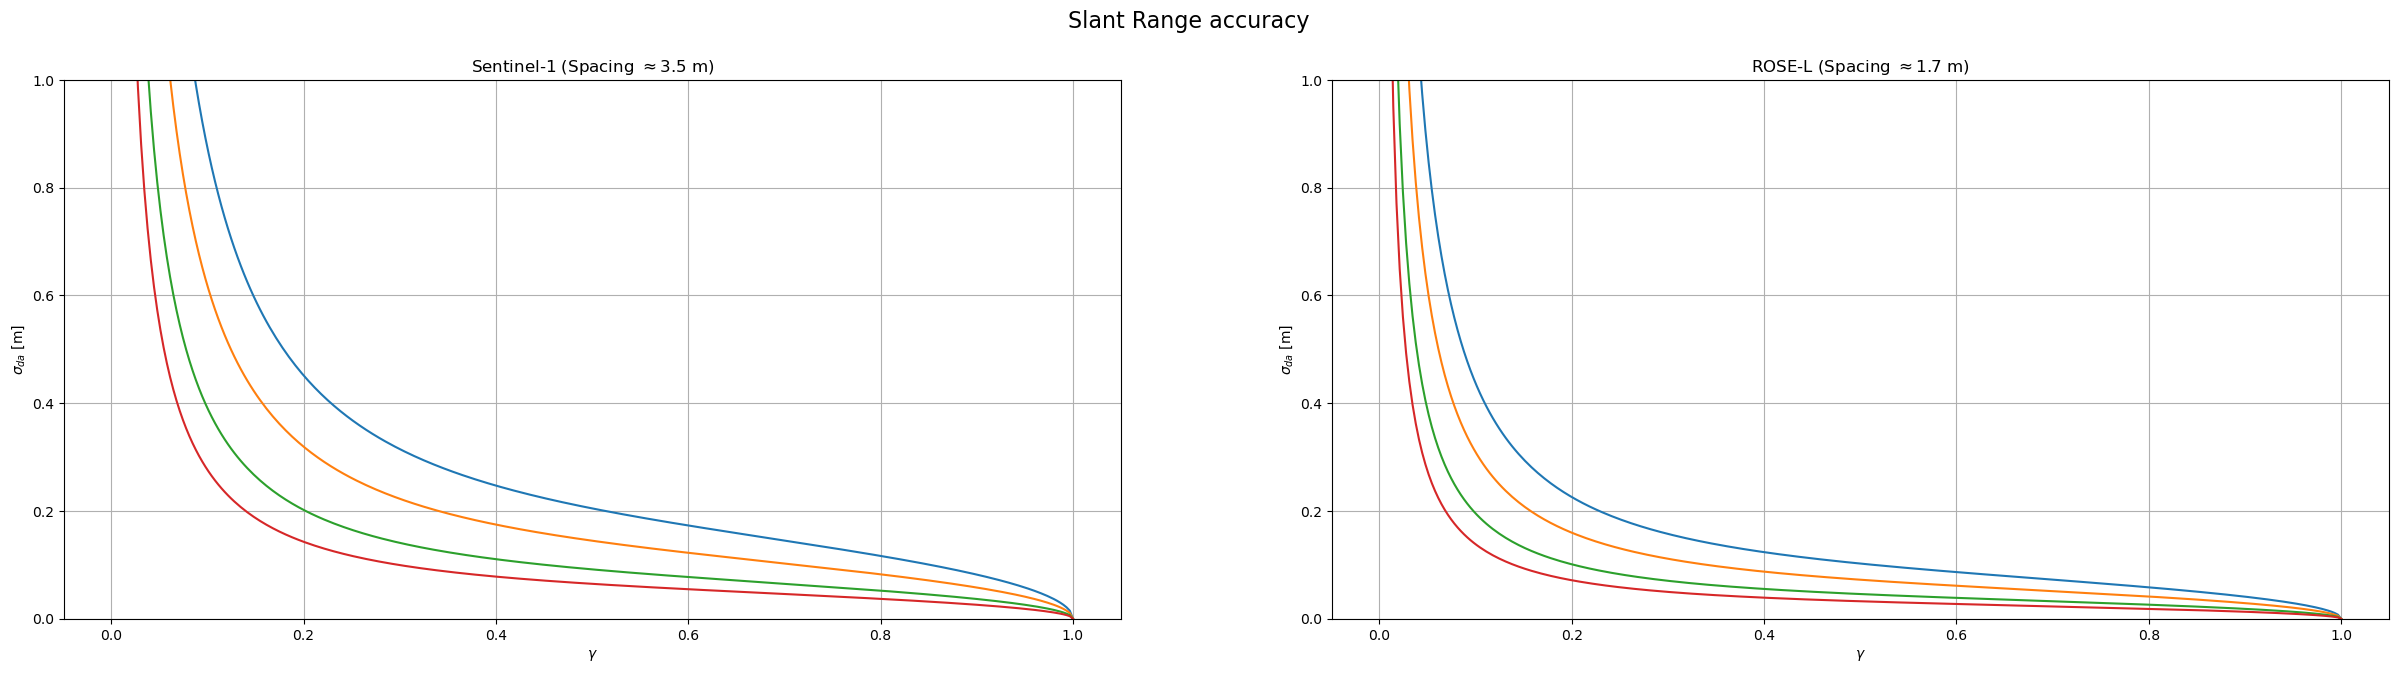
\includegraphics[width=0.9\textwidth]{Figures/pro_pau/rg_accuracy_icc_method.png}
\caption{Estimated slant range displacement accuracy using the incoherent cross-correlation (ICC) method, shown as a function of coherence \(|\gamma|\) for different averaging window sizes \(N\) (represented by color). Left: \acs{s1} configuration. Right: \acs{rosel} configuration. Accuracy is converted from pixels to meters using the corresponding slant-range pixel spacing of each sensor.}
\label{fig:icc_accuracy_slant}
\end{figure}

\begin{figure}[ht!]
\centering
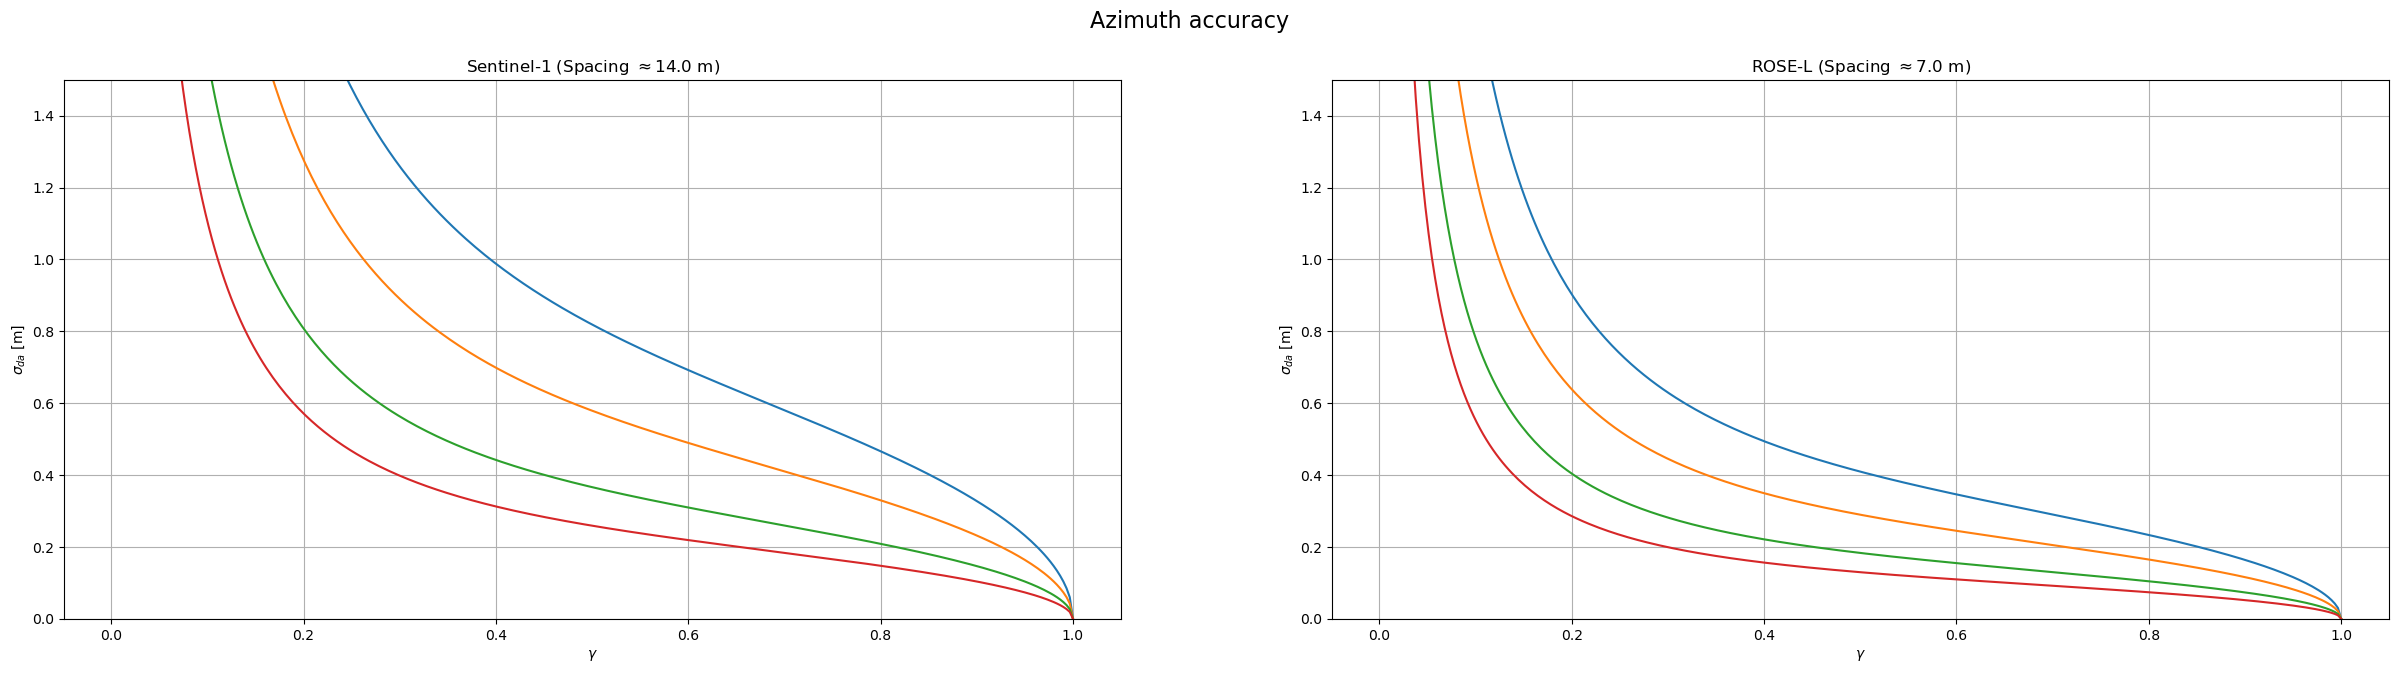
\includegraphics[width=0.9\textwidth]{Figures/pro_pau/az_accuracy_icc_method.png}
\caption{Estimated azimuth displacement accuracy using the incoherent cross-correlation (ICC) method, shown as a function of coherence \(|\gamma|\) for different averaging window sizes \(N\) (represented by color). Left: \acs{s1} configuration. Right: \acs{rosel} configuration. Accuracy is converted from pixels to meters using the respective azimuth pixel spacing of each sensor.}
\label{fig:icc_accuracy_azimuth}
\end{figure}

To illustrate the practical application of the ICC-based method, Figure~\ref{fig:icc_example} shows the estimated displacement field obtained from two \acs{s1} acquisitions over Greenland, separated by 6 days (three consecutive bursts have been used). The displacement vectors were computed using incoherent cross-correlation over a sliding window of 8 pixels in azimuth and 32 pixels in slant range.

Only vectors corresponding to a cross-correlation coefficient greater than 0.4 are shown. Each arrow indicates the direction of the estimated shift, while the color encodes the magnitude of the bidimensional displacement. Despite a notable presence of spurious vectors due to cross-correlation noise—especially in low-texture areas—the majority of the reliable vectors have low magnitude, supporting the assumption of negligible surface motion in this region during the observation period.

\begin{figure}[ht!]
\centering
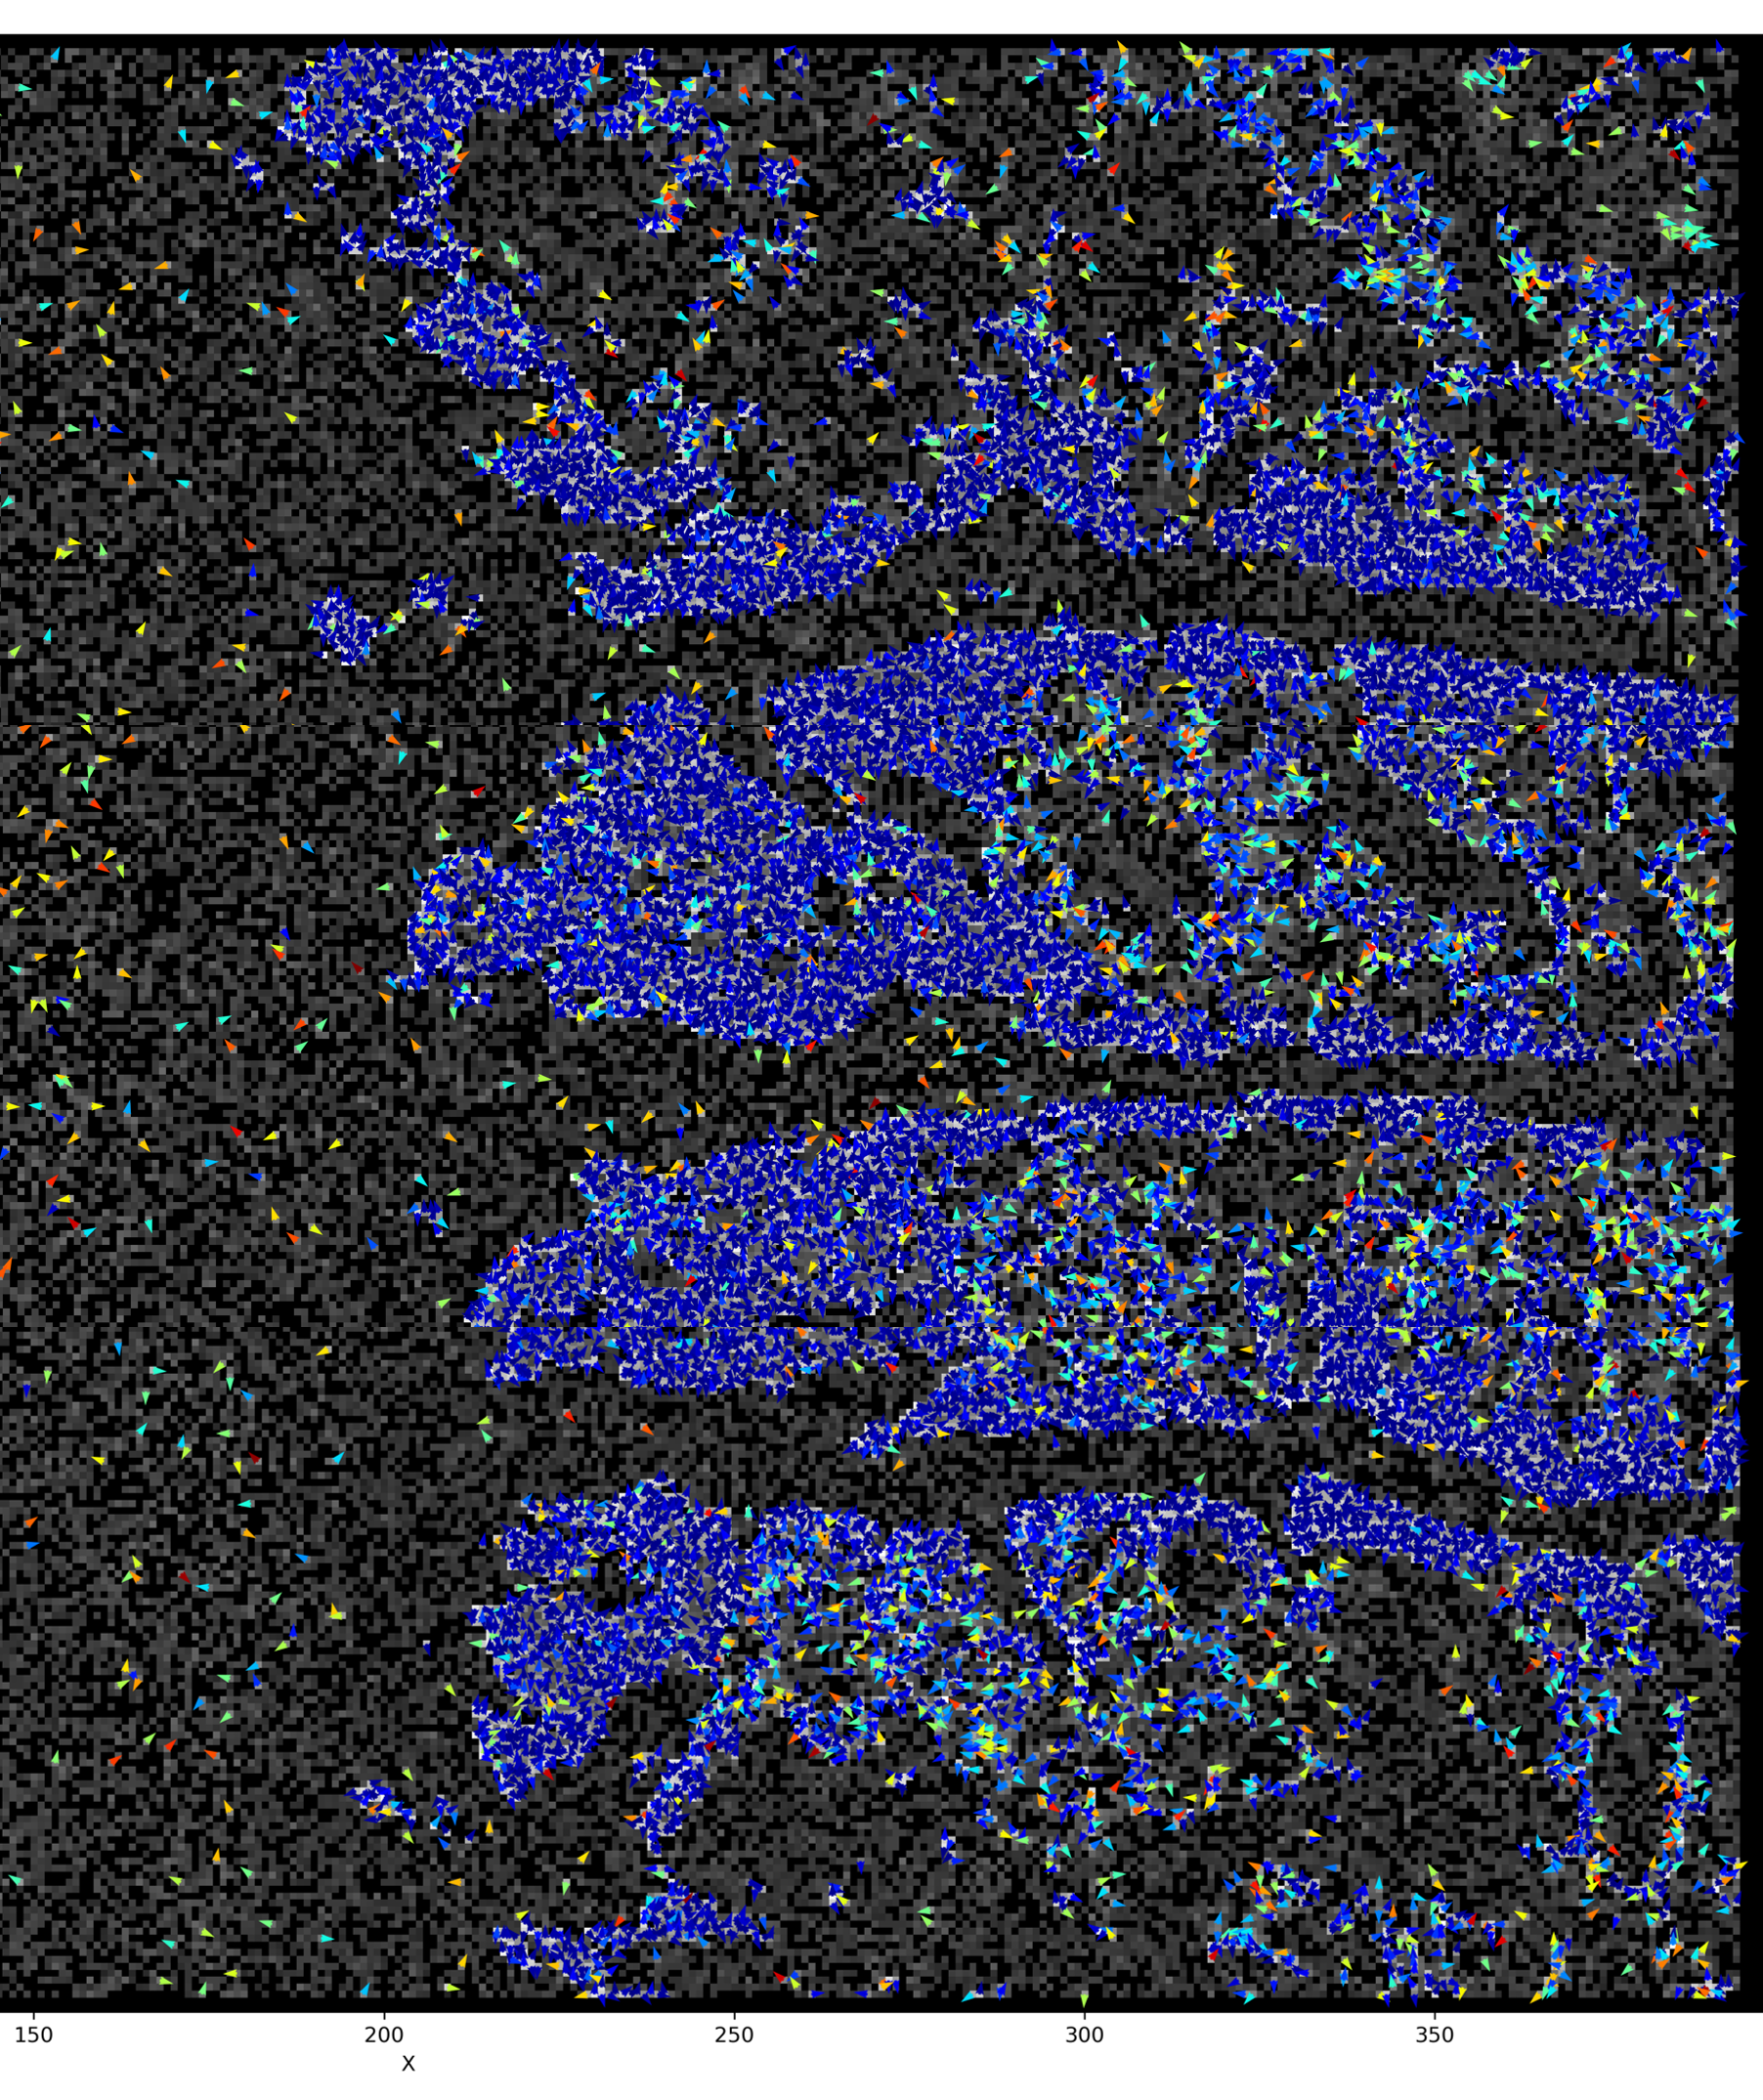
\includegraphics[width=0.8\textwidth]{Figures/pro_pau/icc_example.png}
\caption{Displacement field estimated using the ICC-based method from two Sentinel-1 acquisitions over Greenland, 6 days apart. The image combines three consecutive bursts. Vectors were computed using a cross-correlation window of 8 pixels (azimuth) by 32 pixels (slant range), and only those with a correlation coefficient greater than 0.4 are displayed. Arrow direction indicates the direction of motion, while arrow color represents the magnitude of the estimated bidimensional displacement.}
\label{fig:icc_example}
\end{figure}

\subsection{Computational performance}
\label{sec:pro_pao_computation}

The computational performance of the pixel offset estimation workflow depends significantly on the selected method—phase-based or amplitude-based (ICC)—and on system-specific parameters such as data resolution, overlap area, and window size.

\paragraph{Phase-based estimation}

The phase-based method, which relies on the coherent combination of complex SAR images, is computationally efficient in terms of per-pixel cost but limited in spatial applicability due to the requirement for burst overlap with sufficient Doppler separation. Key steps such as interferogram formation and multilooking are highly optimized and can be parallelized across image tiles. The most computationally intensive component is typically the phase unwrapping stage, particularly in low-coherence regions. However, this cost is mitigated by the fact that significant multilooking is typically applied, which reduces the number of resolution cells to unwrap. As a result, the unwrapping step remains tractable, and the overall processing can be completed in reasonable time. On standard multi-core CPU systems, processing times range from a few seconds to tens of minutes per scene.

\paragraph{ICC-based estimation}

The incoherent cross-correlation (ICC) method can be computationally demanding, especially when applied to large swaths of data. The core of the algorithm involves computing normalized cross-correlation over a sliding window for each valid pixel, followed by sub-pixel peak interpolation. This procedure is repeated independently for each direction (range and azimuth) and can be parallelized both spatially and across bursts. However, memory and I/O demands are non-negligible, particularly when using large windows or high-resolution data such as from \acs{rosel}. The ICC approach scales with the number of search positions and with the window size, making optimization strategies—such as coarse-to-fine search, fast correlation via FFT, and GPU acceleration—highly beneficial. 

\subsection{Criticalities and weakness}
\label{sec:pro_pao_criticalities}

Both phase-based and amplitude-based (ICC) displacement estimation methods are subject to several potential sources of error that must be carefully addressed to ensure reliable measurements. One of the most critical factors affecting the accuracy of displacement estimates—particularly in the slant range direction, but also to a lesser extent in the azimuth direction—is the presence of atmospheric propagation delays.

Tropospheric and ionospheric delays can introduce systematic biases in the measured phase, potentially leading to erroneous displacement estimates. This is especially critical for L-band SAR systems (e.g., \acs{rosel}), where ionospheric effects are more pronounced. Therefore, a fundamental prerequisite for producing reliable \acs{pro} and \acs{pao} products is mitigation of these atmospheric disturbances. Correction strategies include the use of external data—such as ECMWF-based tropospheric delay models or ionospheric delay maps derived from GNSS—or data-driven approaches like the split-spectrum technique, which is particularly effective for isolating ionospheric effects. Regardless of the method used, it is essential to ensure that atmospheric contributions are minimized prior to performing the displacement estimation steps.

In the case of phase-based displacement estimation, an additional critical step is phase unwrapping. This process, which reconstructs the absolute phase from its modulo-\(2\pi\) observations, is inherently complex and highly sensitive to coherence. In areas of low coherence, unwrapping algorithms are prone to errors that can cause entire phase jumps to be missed. Such errors are not local: they can propagate spatially, affecting large areas and introducing displacement artifacts that significantly exceed the noise levels or residual atmospheric effects.

This makes phase unwrapping one of the most failure-prone components in the processing chain when applying the phase-based method. In practice, unwrapping errors can produce large-scale misestimation of displacements, undermining the scientific validity of the results. For this reason, special attention must be paid to both the quality of the coherence map and the robustness of the unwrapping algorithm before accepting phase-derived displacement results as reliable.

\section{Interferometric products (INT / COHE / UNW \& GINT / GCOHE / GUNW)}
\label{sec:int}

The generation of the interferometric product starting from \acs{cslc} is straightforward process. It is assumed that most part of the critical processing have been solved at \acs{cslc} product generation. The only particular step to be executed during the inetrferogram generation is the split-spectrum for the estimation of the ionospheric dispersive component.

\subsection{Evaluation criteria}

\label{sec:int_criteria}

The quality of the interferometric products is evaluated by comparing the outputs generated from \acs{cslc} data with those obtained from a standard processing workflow based on original \acs{slc} data. In particular, we use the ISCE2 software package as a reference processor to generate interferograms from conventional \acs{slc} inputs. Comparison metrics include visual consistency, relative phase structure, coherence levels, and agreement in the phase. 

To assess the fidelity of the interferometric products generated directly from \acs{cslc} data, we performed a benchmark experiment using multiple SAOCOM L-band acquisitions over the Bay of Naples. One image was selected as the reference for co-registration, both in the \acs{cslc} generation pipeline and in the conventional \acs{slc}-based workflow executed with ISCE2. The remaining images were paired with this common reference, resulting in:

\begin{itemize}
  \item a set of long-temporal-baseline interferograms (master–slave separations exceeding three years), and
  \item a set of short-temporal-baseline interferograms (temporal separations shorter than 30 days).
\end{itemize}

Figures~\ref{fig:int_comparison_first} and~\ref{fig:int_comparison_pre} provide two representative examples that allow for a qualitative visual comparison between the results obtained from the \acs{cslc}-based pipeline and those generated using ISCE2. Each figure includes the following:

\begin{enumerate}
  \item \textbf{Left panel}: the wrapped interferogram generated by ISCE2 from the original \acs{slc} data.
  \item \textbf{Centre panel}: the wrapped interferogram obtained by directly applying \(\arg\!\bigl(R \cdot S^{*}\bigr)\) to the pre-generated \acs{cslc} products, where \(R\) and \(S\) refer to the reference and slave images, respectively.
  \item \textbf{Right panel}: the wrapped phase difference \(\arg\bigl(\mathrm{INT}_{\text{ISCE}} \cdot \mathrm{INT}_{\text{CSLC}}^{*}\bigr)\), used to assess potential discrepancies between the two processing chains.
\end{enumerate}

A qualitative inspection leads to the following observations:

\begin{itemize}
  \item Over land, the centre-panel phase difference is essentially flat, indicating that the interferograms produced from \acs{cslc} data are interchangeable with those generated by the well-established ISCE2 workflow.
  \item Over the sea, fringe patterns appear in the difference maps. These originate from a processing divergence rather than an error: ISCE2 embeds bathymetric information when flattening the phase before forming the interferogram, whereas the \acs{cslc}-based chain assumes a zero-elevation (sea-level) surface. Consequently, the difference field over water represents the negated bathymetric phase term included only in the ISCE2 product.
  \item No systematic residuals linked to temporal baseline length are evident, confirming that the \acs{cslc} generation has preserved the phase stability required for both short- and long-baseline interferometry.
\end{itemize}

The experiment therefore demonstrates that interferograms computed from \acs{cslc} inputs preserve the scientific quality of those generated from \acs{slc} data, while offering the processing simplifications and storage benefits inherent to the \acs{cslc} format.

\begin{figure}[ht!]
  \centering
  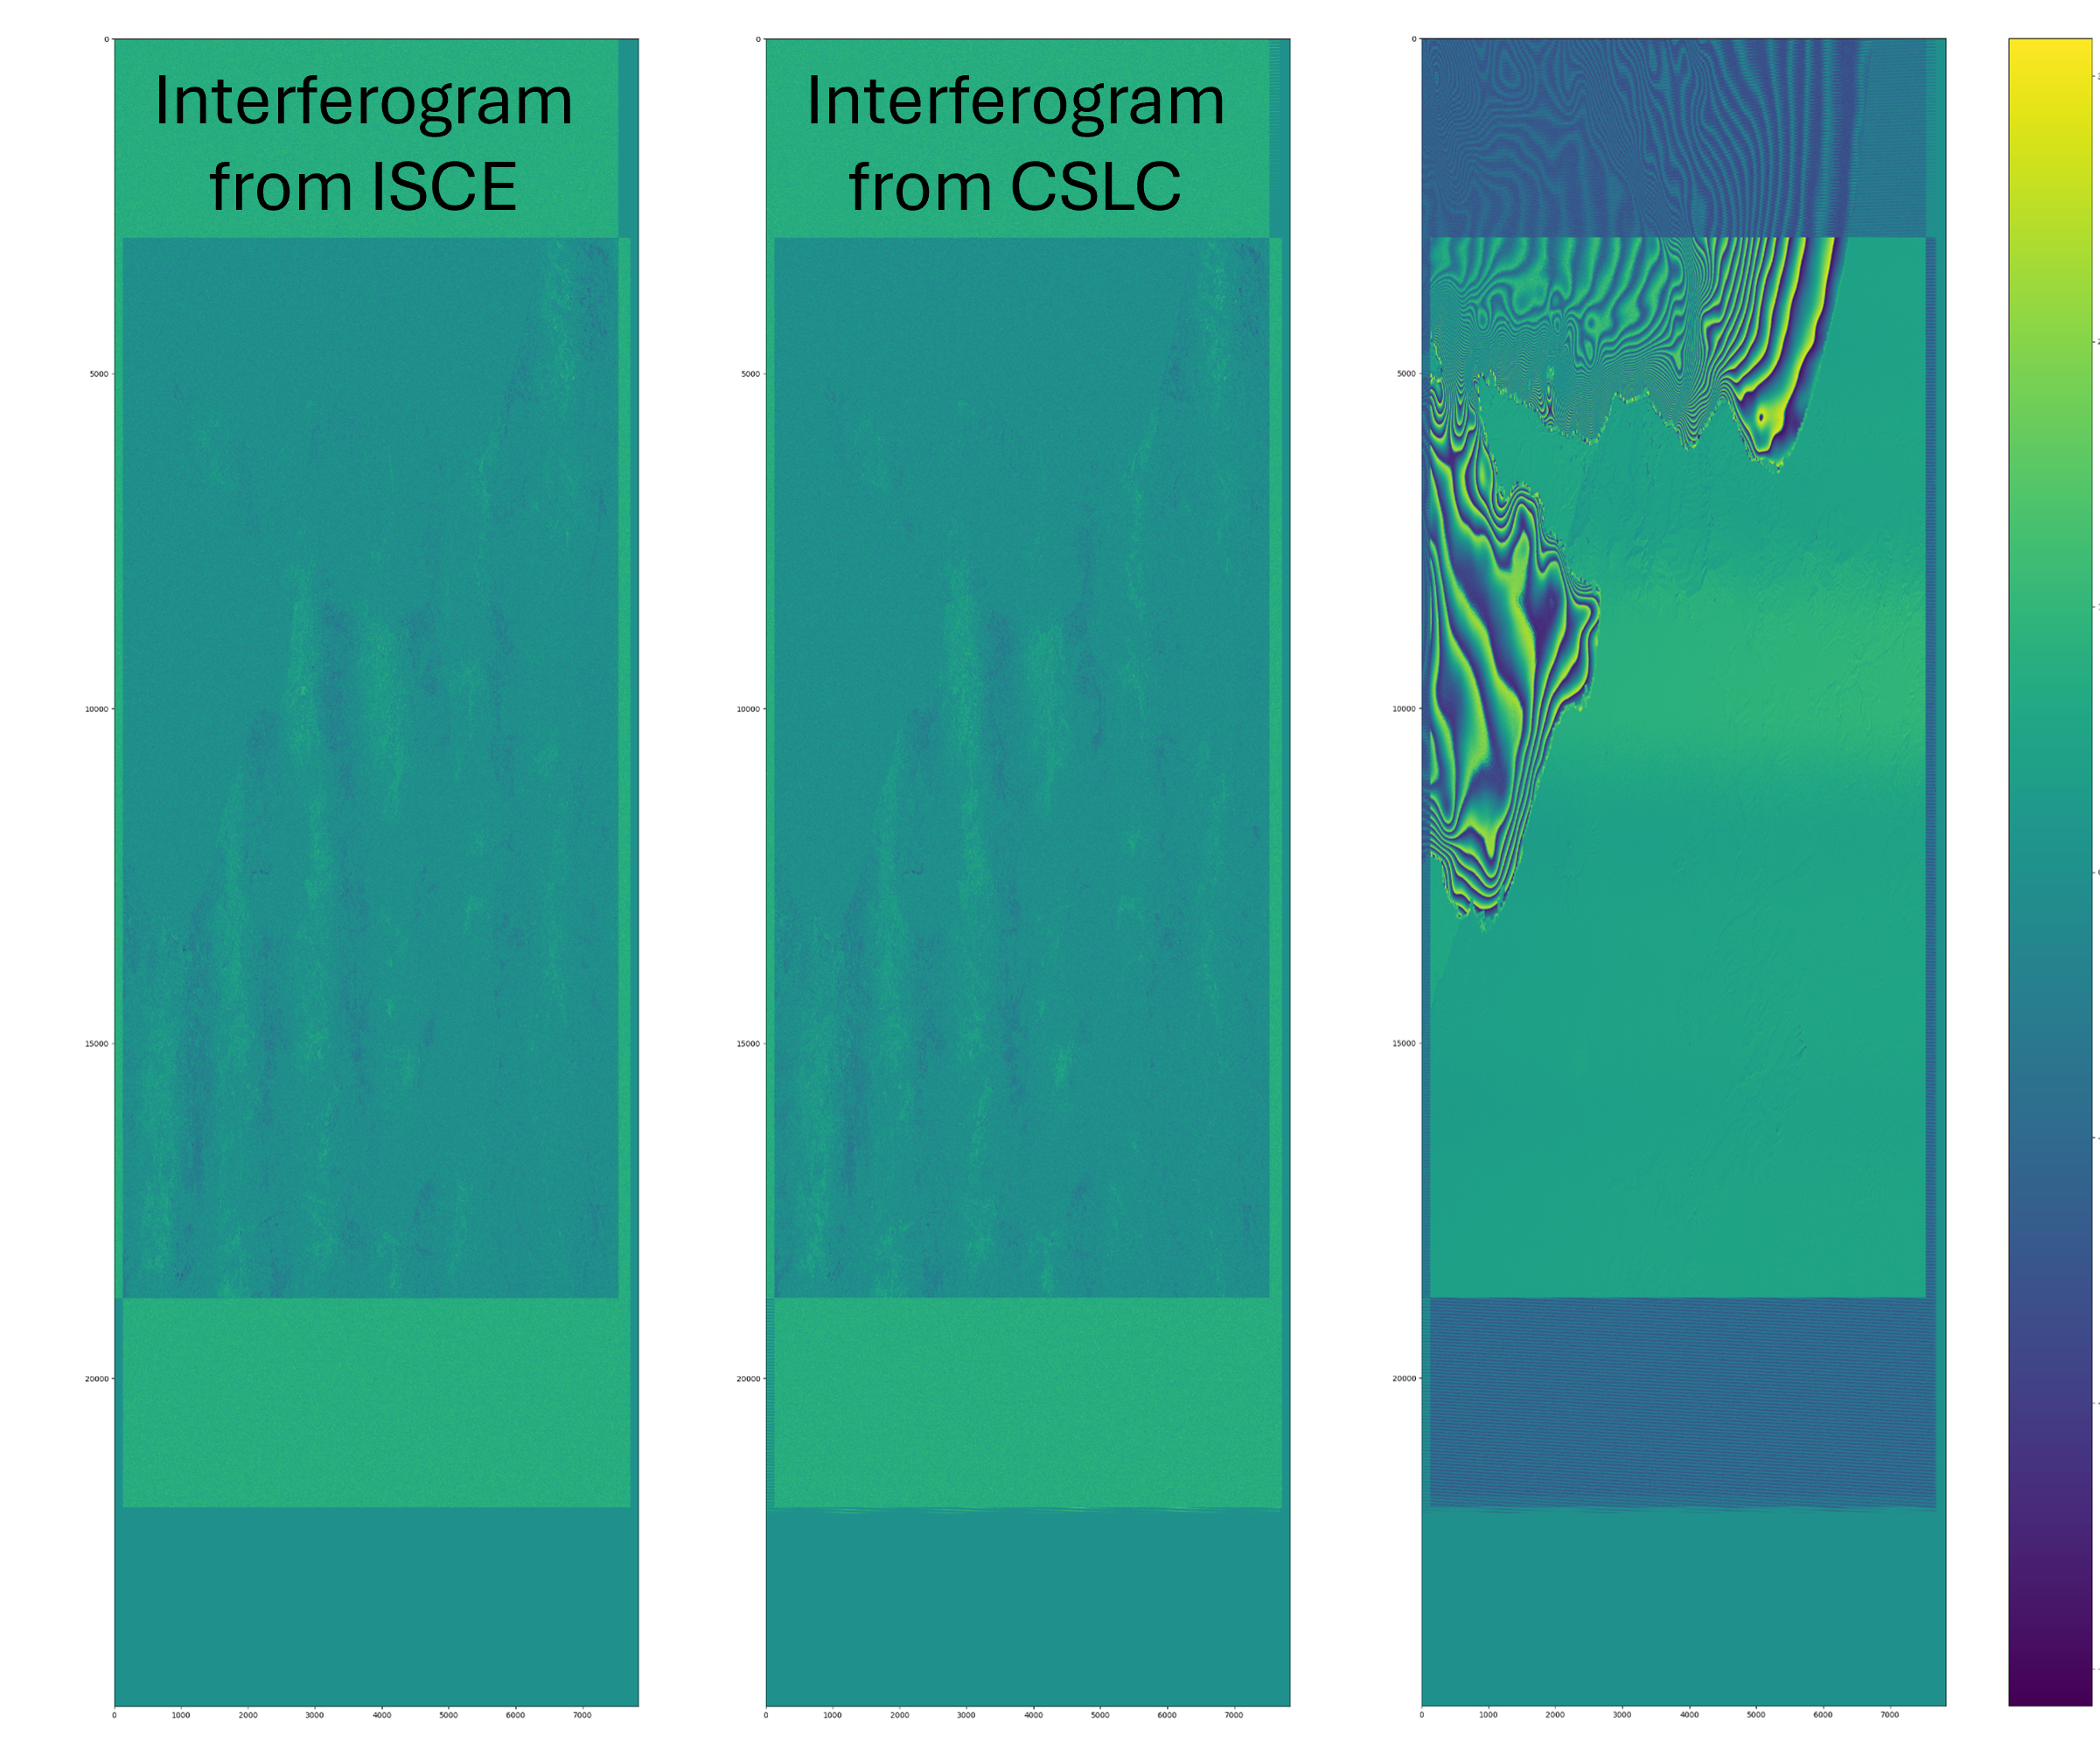
\includegraphics[width=\textwidth]{Figures/interf/comparison_first.png}
  \caption{Comparison of interferograms generated using the \acs{cslc}-based pipeline and ISCE2 for a long-temporal-baseline pair. The master image was acquired on 2023-12-12, and the slave image on 2020-04-23, resulting in a temporal separation of more than three years. Left: interferogram produced by ISCE2 from \acs{slc} data. Centre: wrapped interferogram computed directly from \acs{cslc} products. Right: wrapped phase difference between ISCE2 and \acs{cslc} results.}
  \label{fig:int_comparison_first}
\end{figure}

\begin{figure}[ht!]
  \centering
  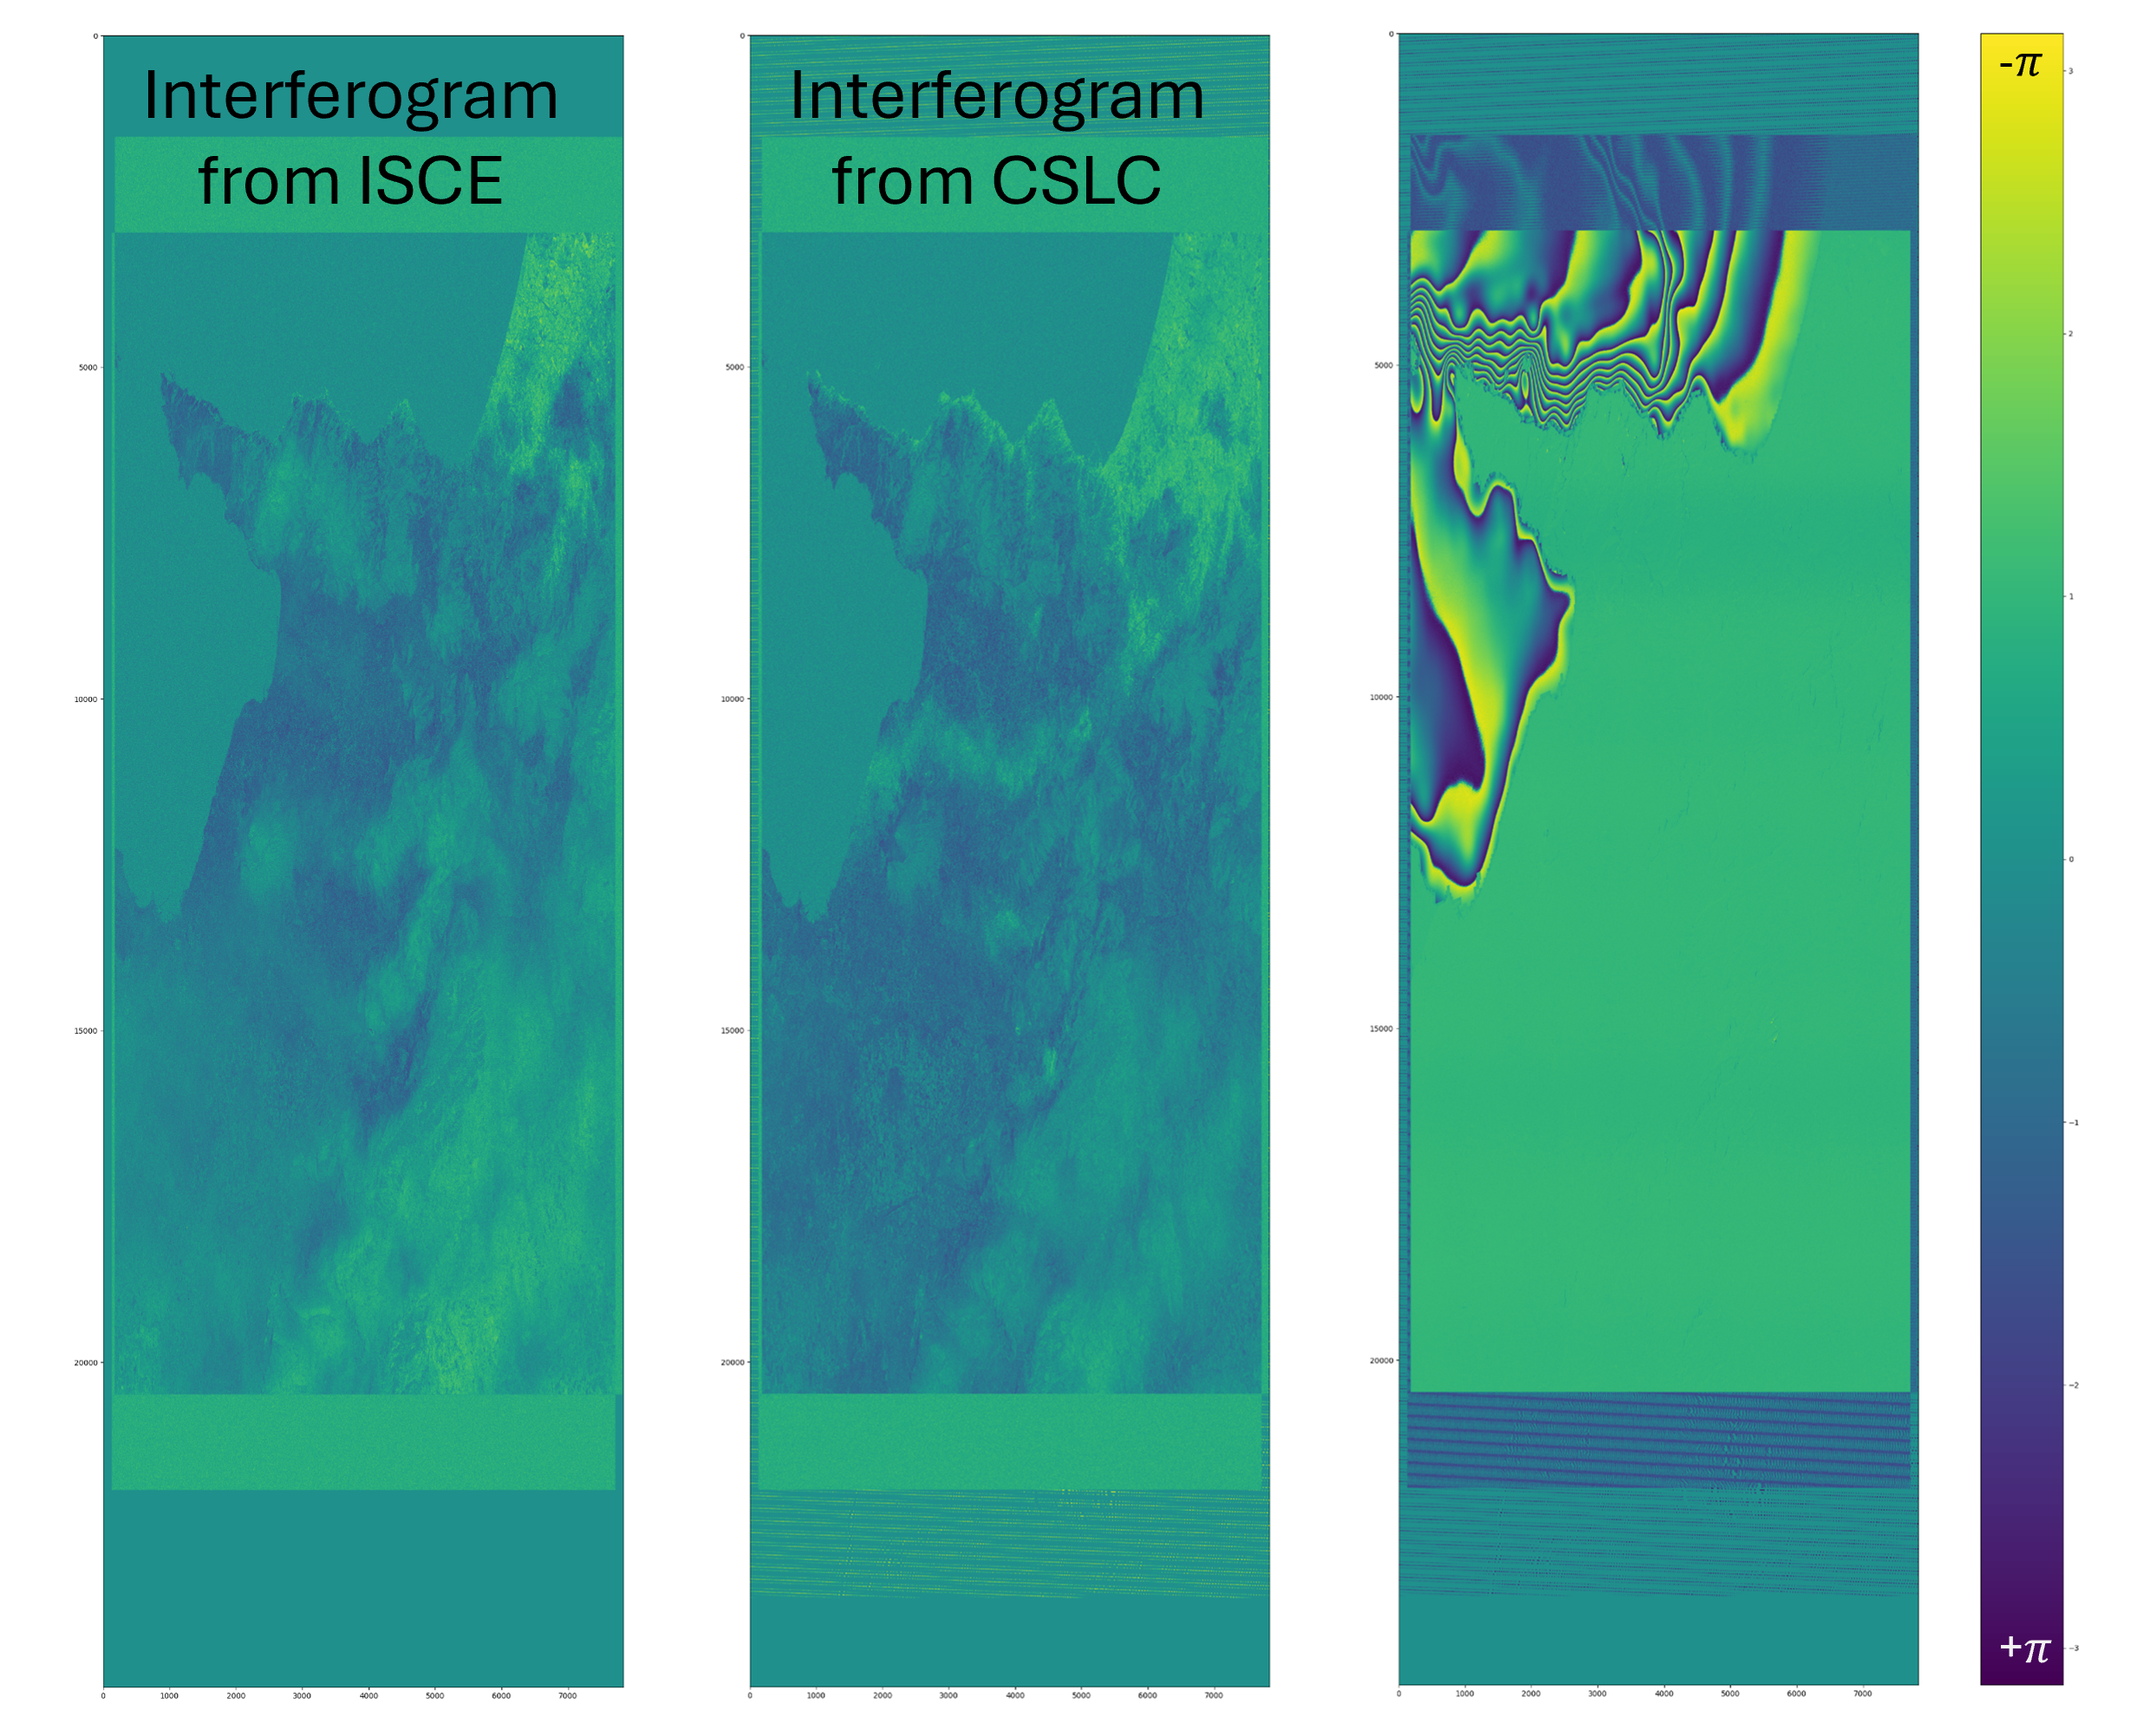
\includegraphics[width=\textwidth]{Figures/interf/comparison_pre.png}
  \caption{Comparison of interferograms generated using the \acs{cslc}-based pipeline and ISCE2 for a short-temporal-baseline pair. The master image was acquired on 2023-12-12, and the slave image on 2023-11-18, resulting in a 25-day temporal separation. Left: interferogram produced by ISCE2 from \acs{slc} data. Centre: wrapped interferogram computed directly from \acs{cslc} products. Right: wrapped phase difference between ISCE2 and \acs{cslc} results.}
  \label{fig:int_comparison_pre}
\end{figure}

In addition to the phase comparison, we also evaluated the coherence maps produced from the same image pairs. Specifically, we compared the coherence computed from the \acs{cslc}-based pipeline with that obtained using ISCE2. In both cases, coherence was estimated using square windows corresponding to approximately 100 meters in both range and azimuth directions.

Figures~\ref{fig:coh_comparison_short} and~\ref{fig:coh_comparison_long} show the results for the same two image pairs previously used for the interferometric phase analysis: one short-temporal-baseline pair (25 days) and one long-temporal-baseline pair (more than three years). Each figure consists of the following panels:

\begin{enumerate}
  \item \textbf{Left panel}: coherence map produced by ISCE2 from the original \acs{slc} data.
  \item \textbf{Centre panel}: coherence map derived from the \acs{cslc} products using the same processing parameters.
  \item \textbf{Right panel}: pixel-wise difference map, computed as (ISCE coherence) minus (CSLC-based coherence).
\end{enumerate}

The two examples clearly show that the coherence values are generally consistent between the two processing chains. Minor differences are visible, particularly in the form of horizontal striping in the difference maps, where the \acs{cslc}-based pipeline appears to yield slightly higher coherence values. This behavior suggests localized inconsistencies in the ISCE processing, which may slightly degrade coherence quality in specific areas. 

In addition, Figure~\ref{fig:coh_diff_histograms} reports the histograms of the pixel-wise coherence differences for both interferogram pairs. The histograms confirm that the differences are centered around zero and generally small in magnitude, indicating that the \acs{cslc}-based coherence maps are qualitatively equivalent to those obtained using ISCE2.

\begin{figure}[ht!]
  \centering
  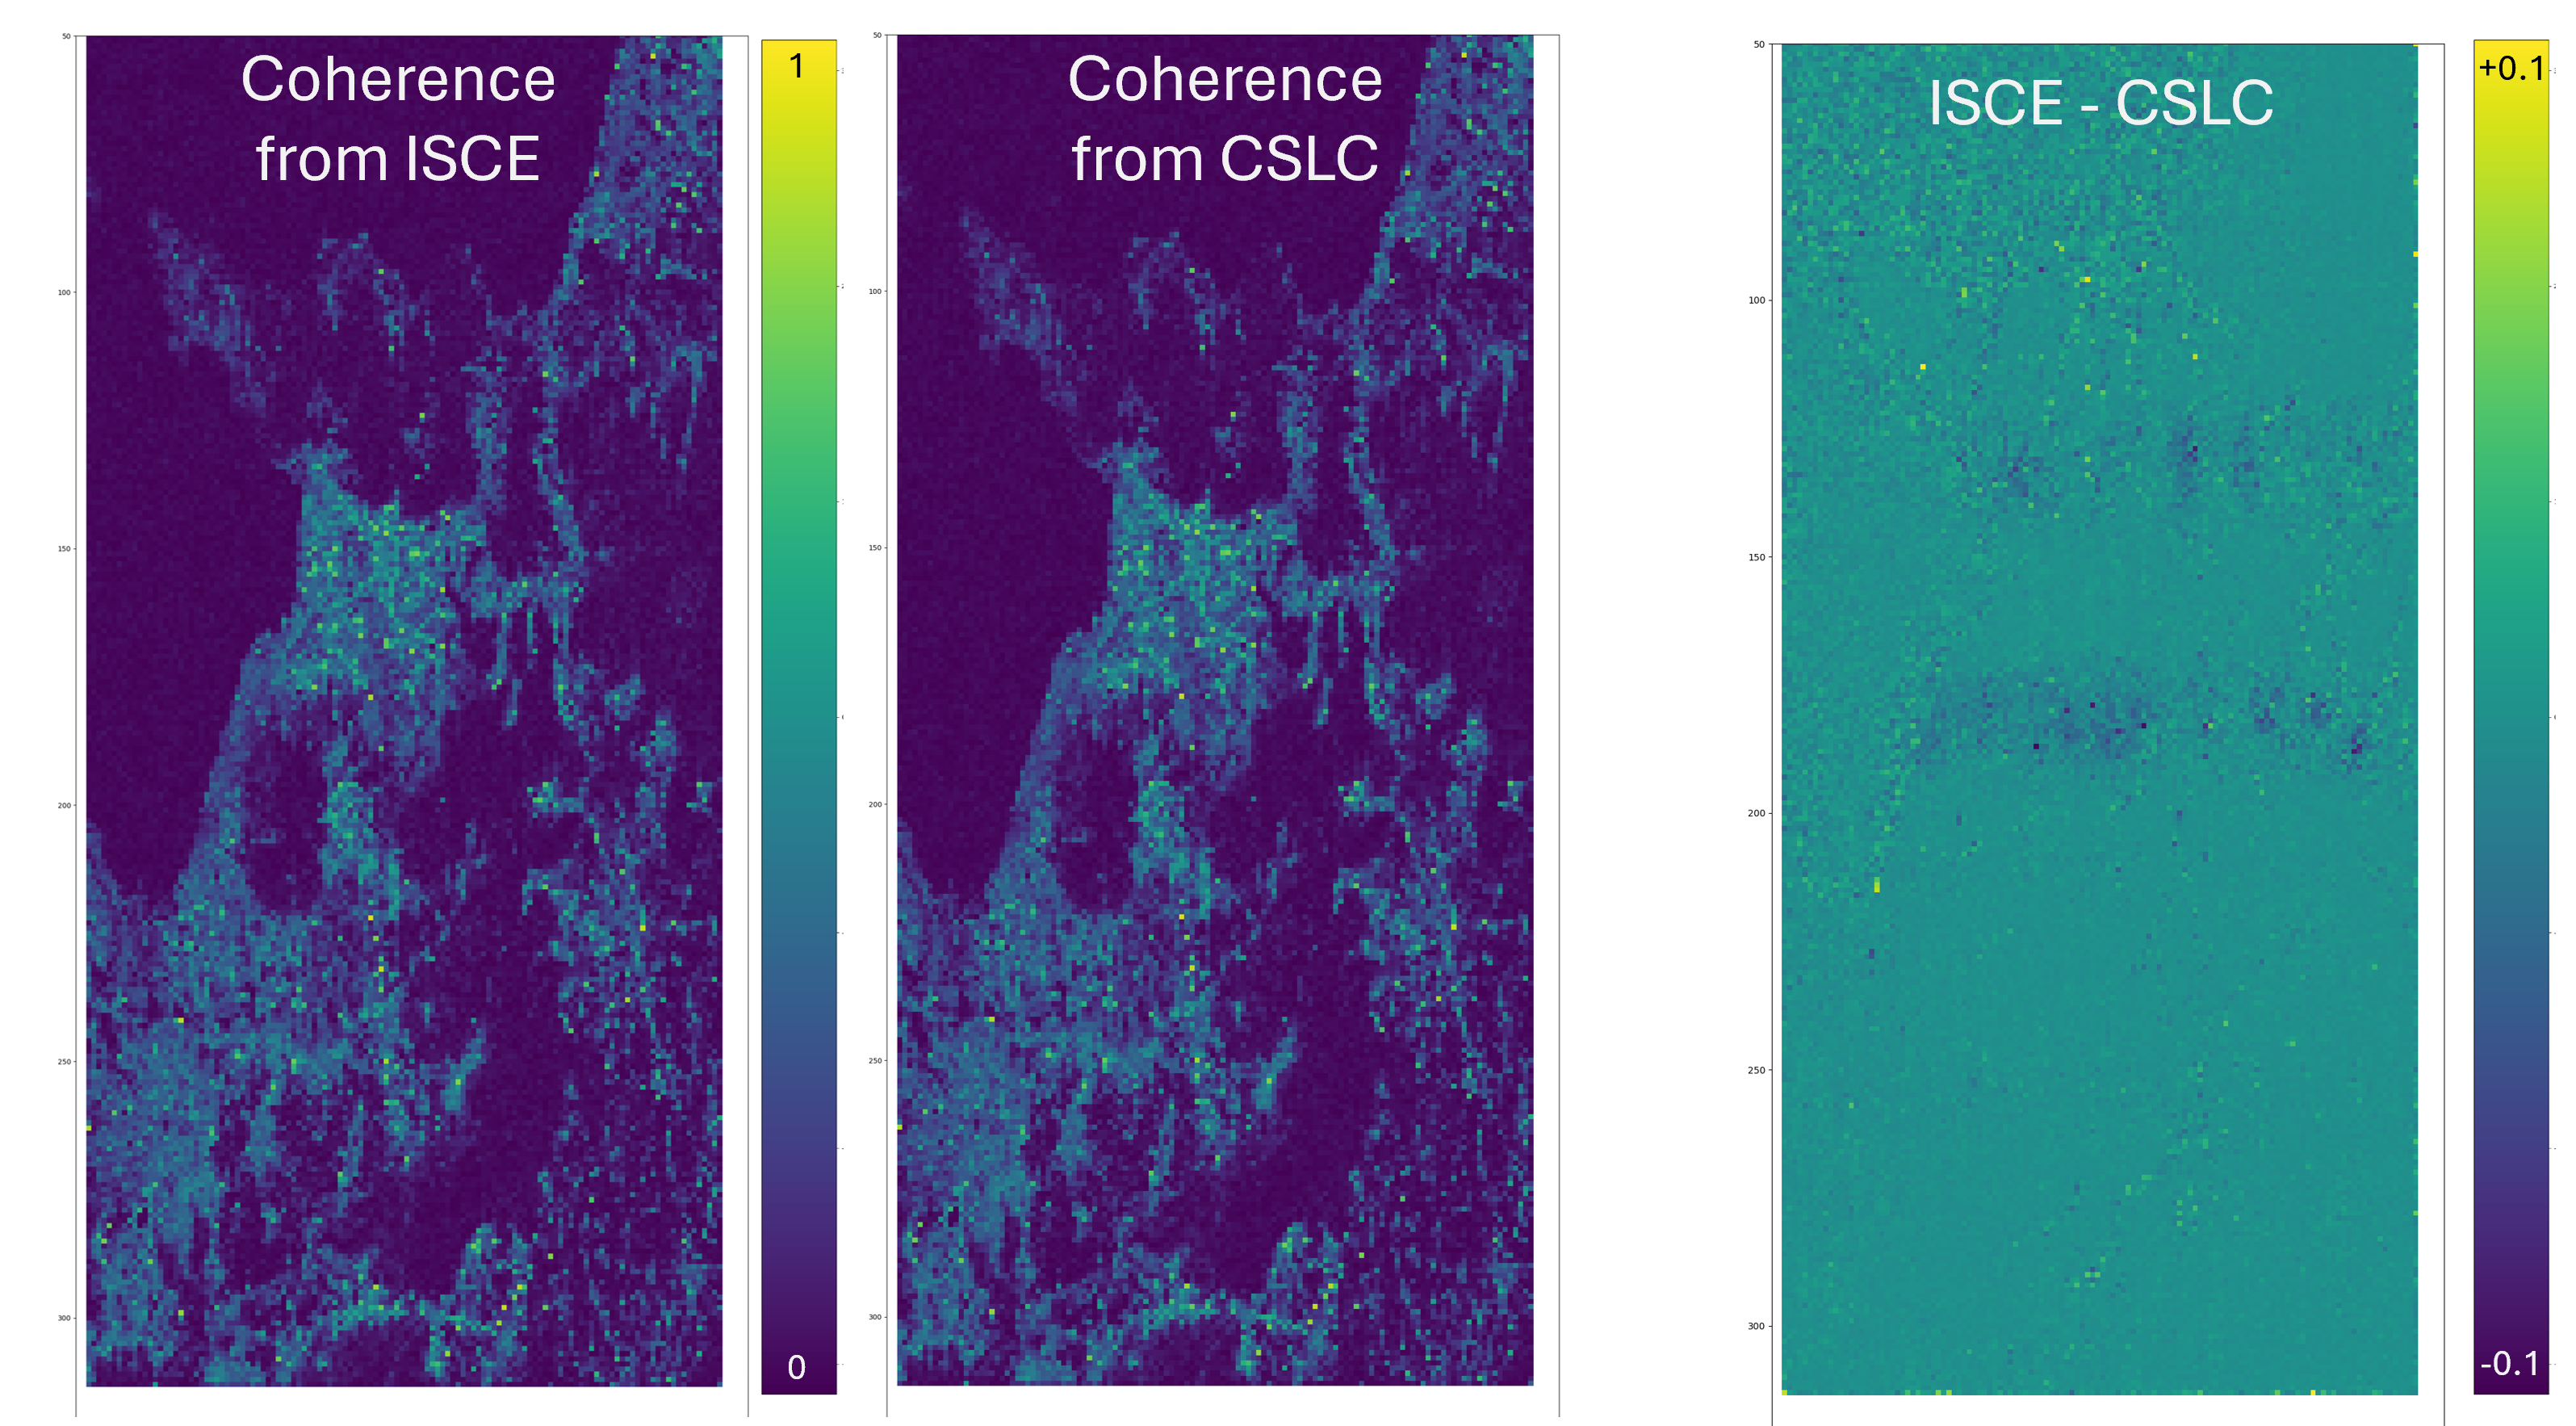
\includegraphics[width=\textwidth]{Figures/interf/coh_comparison_long.png}
  \caption{Comparison of coherence maps computed from a long-temporal-baseline image pair (more than three years). Left: ISCE2 coherence from \acs{slc} data. Centre: coherence computed from \acs{cslc} products. Right: pixel-wise difference (ISCE – CSLC).}
  \label{fig:coh_comparison_long}
\end{figure}

\begin{figure}[ht!]
  \centering
  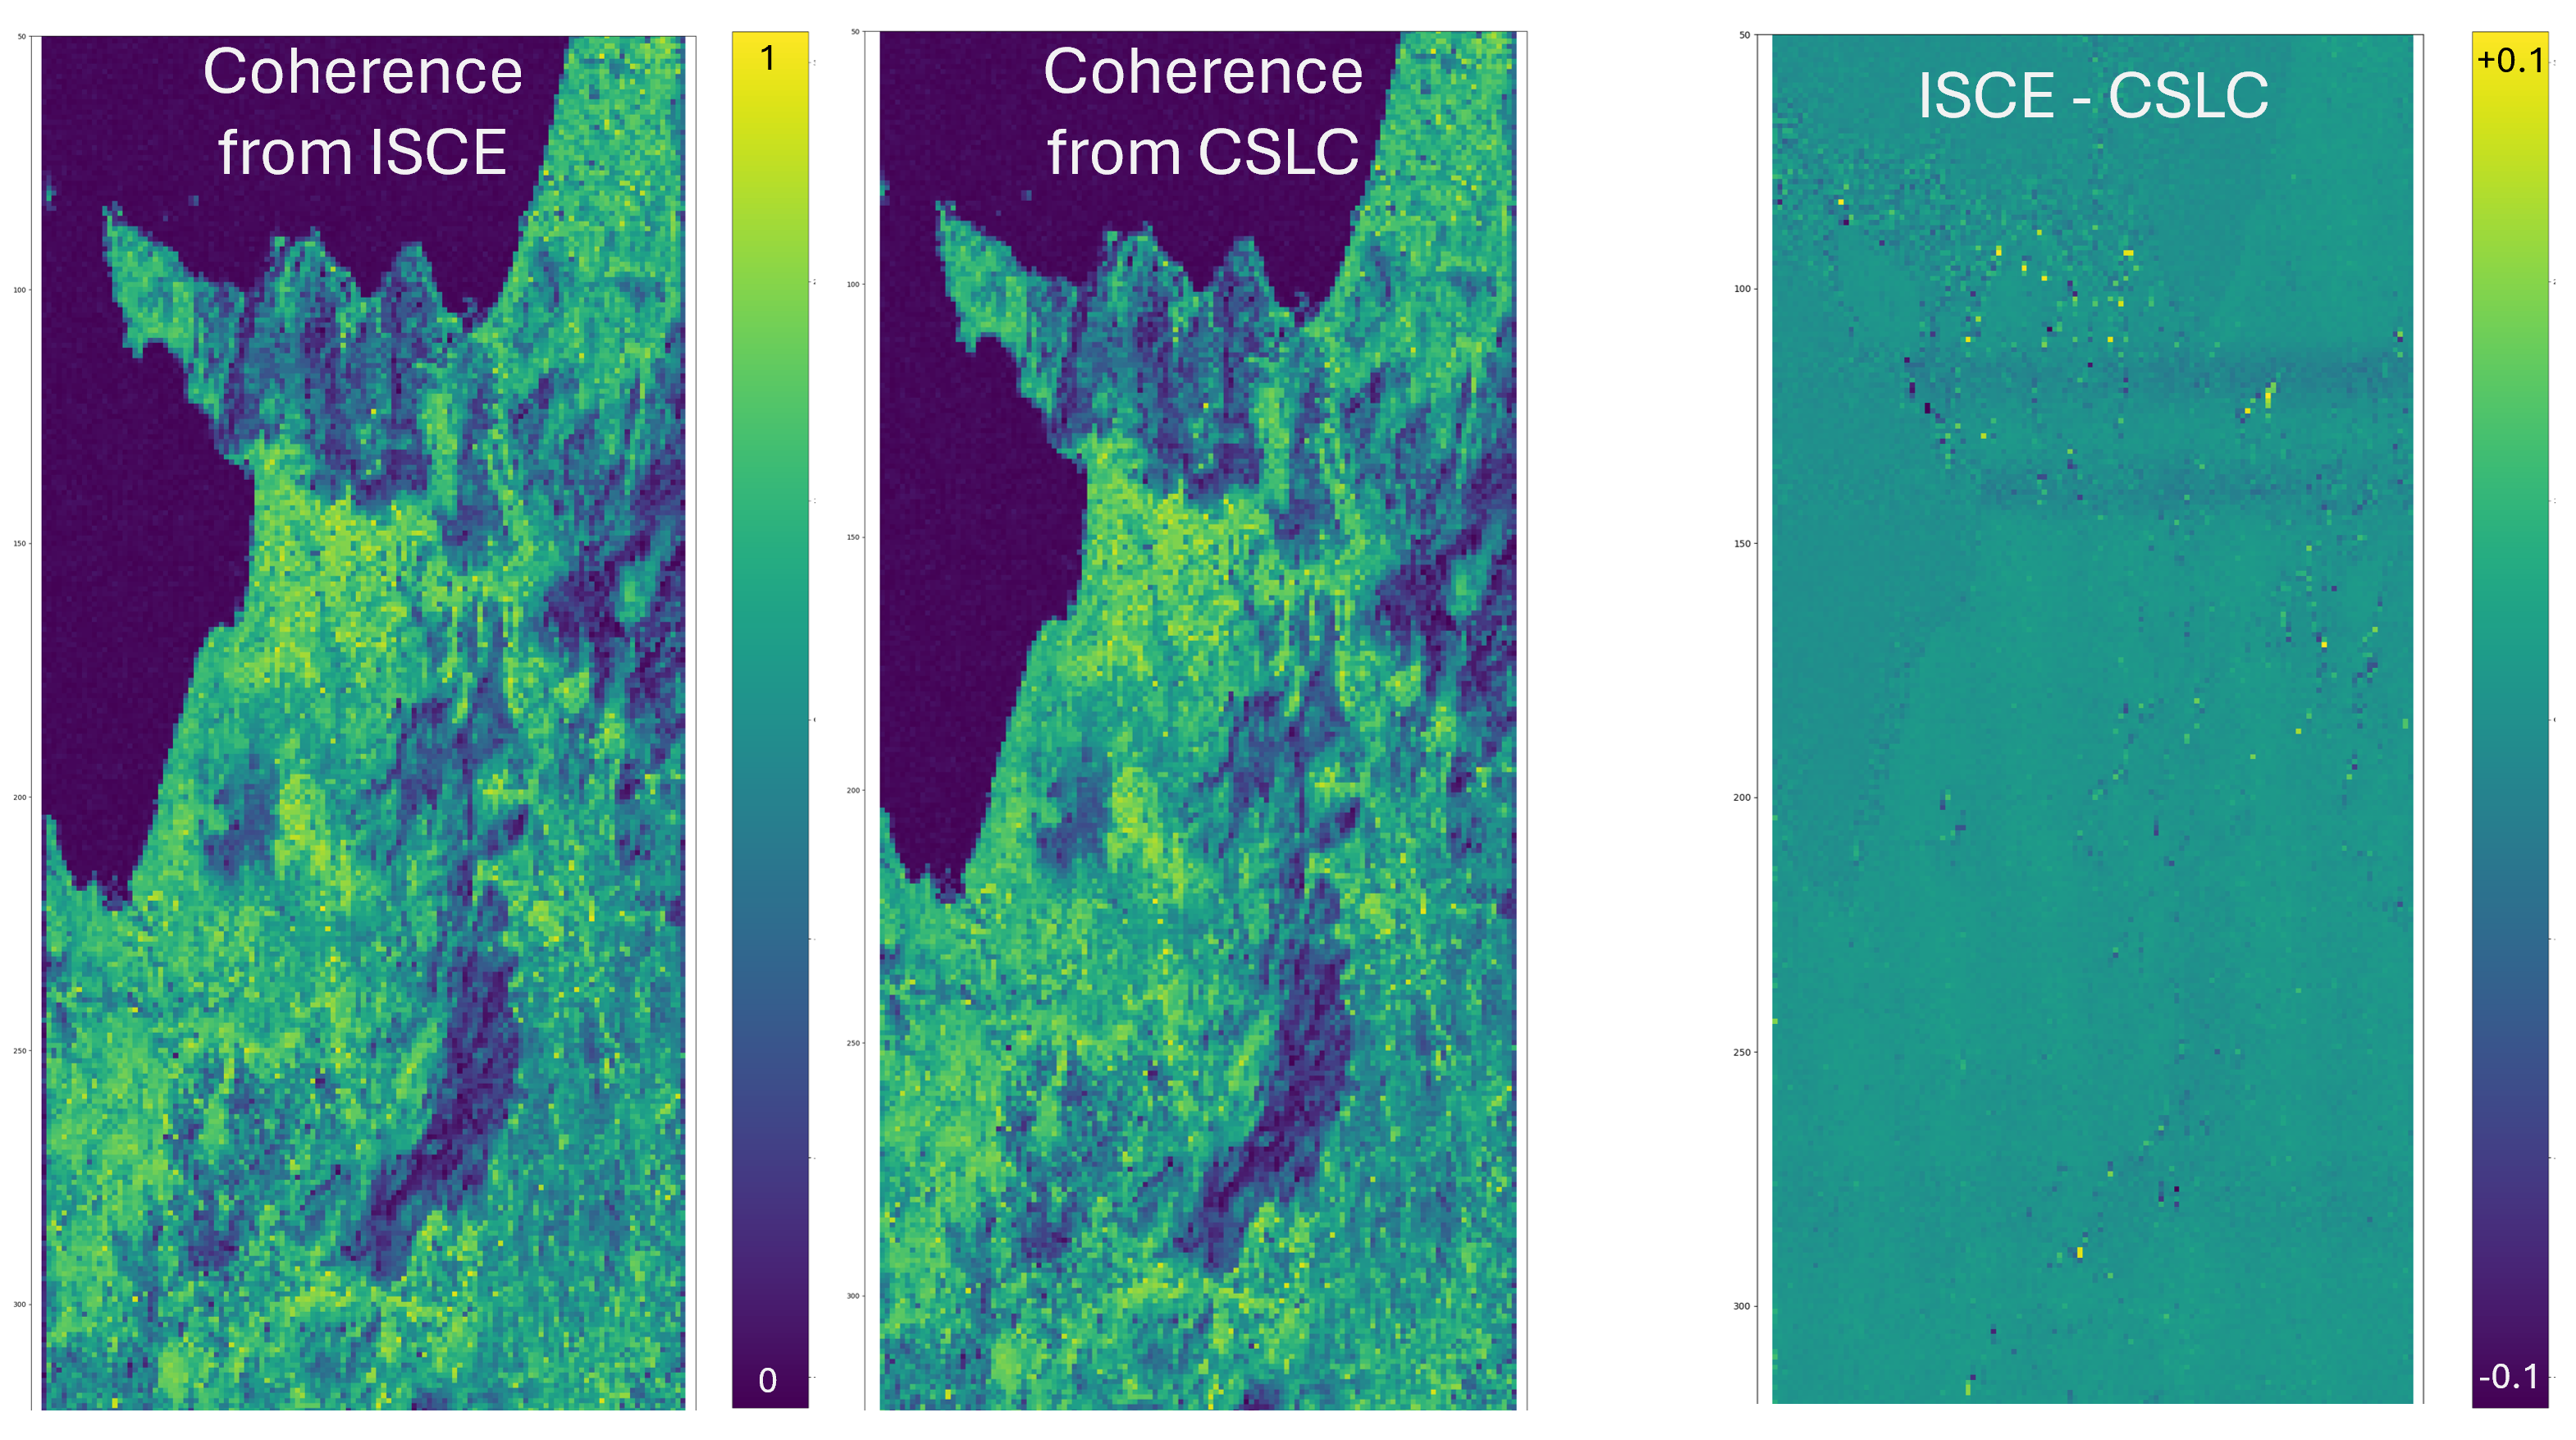
\includegraphics[width=\textwidth]{Figures/interf/coh_comparison_short.png}
  \caption{Comparison of coherence maps computed from a short-temporal-baseline image pair (25 days). Left: ISCE2 coherence from \acs{slc} data. Centre: coherence computed from \acs{cslc} products. Right: pixel-wise difference (ISCE – CSLC).}
  \label{fig:coh_comparison_short}
\end{figure}

\begin{figure}[ht!]
  \centering
  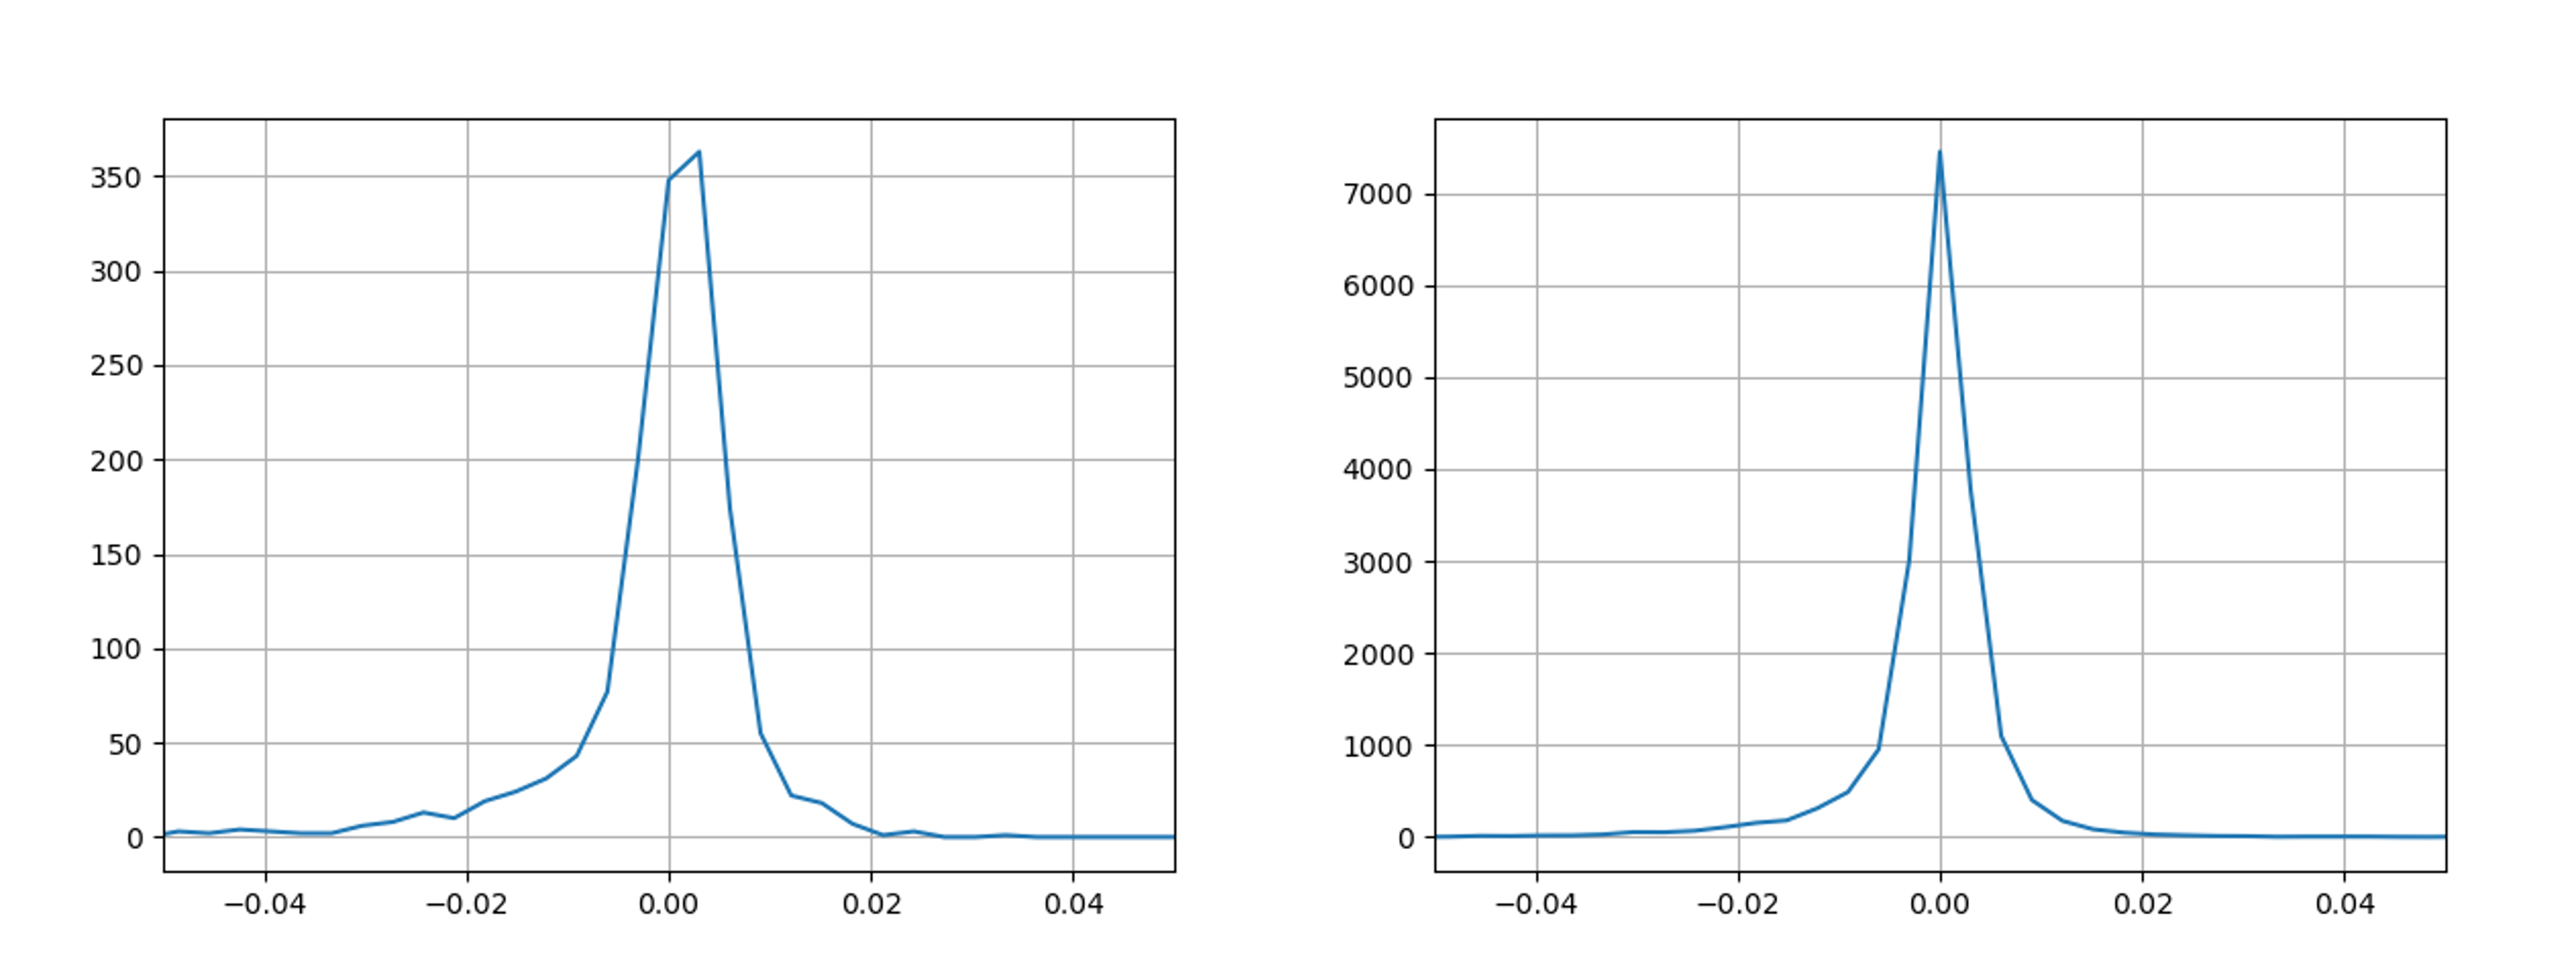
\includegraphics[width=\textwidth]{Figures/interf/istogramma_diff_first_left__pre_rigth.png}
  \caption{Histograms of the pixel-wise differences between the ISCE2 and \acs{cslc}-based coherence maps for the two image pairs (long, on the left, and short, on the right, temporal baseline). The distributions confirm that the coherence estimates from both approaches are statistically equivalent.}
  \label{fig:coh_diff_histograms}
\end{figure}

\subsection{Computational performance}
\label{sec:int_computation}
Generating the interferogram involves multiplying two complex-valued images and applying filters to reduce noise. This operation is simple, and its computational cost is proportional to the number of pixels in the input images.

The most demanding steps are split-spectrum processing and phase unwrapping. However, by using multilooked data, it is possible to significantly reduce the computational cost.

At the moment, another computationally expensive step is geocoding. This cost is the same of the \acs{nrb} product. In fact, the geocoding method is based on the same projection matrix used in the area-projection algorithm. The cost could be reduced by adopting a geocoding strategy tailored to multilooked data.

\subsection{Criticalities and weakness}
\label{sec:int_criticalities}

Interferometric products inherit the criticalities and weaknesses of the \acs{cslc} product.

\subsection{Data Generation}
\label{sec:int_data_generation}
The ISCE environment can be created using
\begin{lstlisting}[language=bash]  
conda install conda-forge::isce2
\end{lstlisting}
and the creation is performed by typing the following line:
\begin{lstlisting}[language=bash]  
yourEnv/lib/python3.11/site-packages/isce/applications/stripmapApp.py
--steps yourPath/StripmapAppSAOCOM.xml 2$>&1$ | tee SAOCOM
\end{lstlisting}
Attention must be paid in substituting \emph{yourEnv} and \emph{yourPath} with the correct paths.

Hereafter there is an example of \emph{StripmapAppSAOCOM.xml} file.

\begin{lstlisting}[language=xml]  
<?xml version="1.0" encoding="UTF-8"?>
<insarApp>
  <component name="insar">
    <property name="sensor name">SAOCOM_SLC</property>
    <component name="reference">
        <catalog>/home/debora/tests_Naples/test_pre_master/
            reference_SAOCOM.xml</catalog>
    </component>
    <component name="secondary">
        <catalog>/home/debora/tests_Naples/test_pre_master/
            secondary_SAOCOM.xml</catalog>
    </component>
    <property name="demFilename">
        <value>/home/debora/tests_Naples/demLat_40_S42_Lon_W013
            _W016.dem.wgs84</value>
    </property>
    <property name="do denseoffsets">True</property>
    <property name="do split spectrum">True</property>
    <property name="unwrapper name">snaphu</property>
    <property name="do dispersive">True</property>
    <property name="dispersive filter kernel x-size">800</property>
    <property name="dispersive filter kernel y-size">800</property>
    <property name="dispersive filter kernel sigma_x">100</property>
    <property name="dispersive filter kernel sigma_y">100</property>
    <property name="dispersive filter kernel rotation">0</property>
    <property name="dispersive filter number of iterations">5</property>
    <property name="dispersive filter mask type">connected_components</property>
    <property name="dispersive filter coherence threshold">0.6</property>

  </component>
</insarApp>
\end{lstlisting}

The \emph{dem} file can be created by typing
\begin{lstlisting}[language=bash]  
yourEnv/lib/python3.11/site-packages/isce/applications/dem.py -a 
stitch -b 39 42 13 16 -r -s 1 -c -o 
demLat_39_S42_Lon_W013_W016.dem.wgs84 --dir /yourPath
\end{lstlisting}
using the coordinates of the area of interest.






\section{Co-registered and geocoded MLC (CMLC \& GMLC)}
\label{sec:cmlc}

\subsection{Evaluation criteria}
\label{sec:cmlc_criteria}

We are proposing here to assess the performance of the phase products in two ways, i.e. by analyzing
\begin{itemize}
    \item The relative performance with real data by comparing with other phase estimators applied to the same data,
    \item The absolute performance by evaluating the algorithms on synthetic data.
\end{itemize}
In the second case, we are also going to develop a theoretical model to describe the coherence of interferograms which are generated internally by the progressive phase estimation algorithm.

The first approach has the advantage of situating the performance of the new algorithm with respect to known alternatives. It works on real data and thus maximizes the relevance for real-life applications.

The second approach has the advantage of checking the absolute performance and the behavior for specific, possibly critical, scenarios which might not be represented by the real-data dataset available for the study.

A more complete validation of the product would require further high-level processing to obtain deformation time series, which could then be compared to other products and sensors, like EGMS (European Ground Motion Service) or GNSS series. To do this in a proper way, one should also include atmospheric corrections, especially tropospheric ones. 
Despite the increased effort, a validation of this kind is going to have some limitations too: the differences between the sensors are going to result in different levels of noise, both on single measurements and on the mean velocity.
The activity should be understood more in terms of cross-comparison than pure validation.

This effort is, however, not necessary if we want to verify the core phase-estimation part, which is anyway the most critical and innovative contribution introduced in this project. Once the phase is well estimated, subsequent processing can follow the traditional PS/DS approach, including phase unwrapping and atmospheric corrections, which is well understood and validated.

\subsection{Relative performance assessment (SAOCOM)}
The algorithm for the generation of the MLC product is described in ATBD, let us call it progressive interferometric phase estimation (PIPE). In the plots, we are indicating it simply with "cmlc". The auto-regressive parameter for the running reference is chosen to be 0.95, whereas the long-term reference is a fixed snapshot of the running reference taken at the 10th acquisition.

We are going to discuss its performance with respect to
\begin{enumerate}
    \item EMI, a full-covariance phase estimation method (\cite{Ansari2018}),
    \item direct interferograms (indicated with "direct" in the plots),
    \item a version of progressive estimation without drift control and with fast-fading memory (indicated with "ndc", i.e. "no drift control", in the plots), to show a degraded performance.
\end{enumerate}


\begin{figure}[ht]
    \centering
    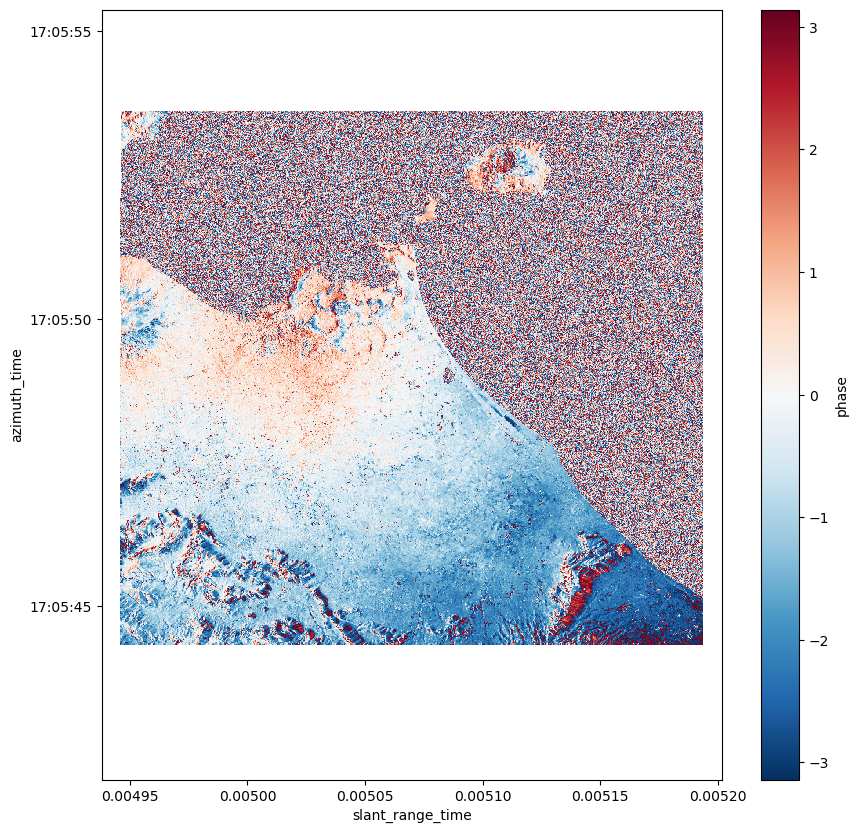
\includegraphics[width=0.45\linewidth]{Figures/mlc/DSC_S4/2025-01-14_2015-01-30_pipe.png}
    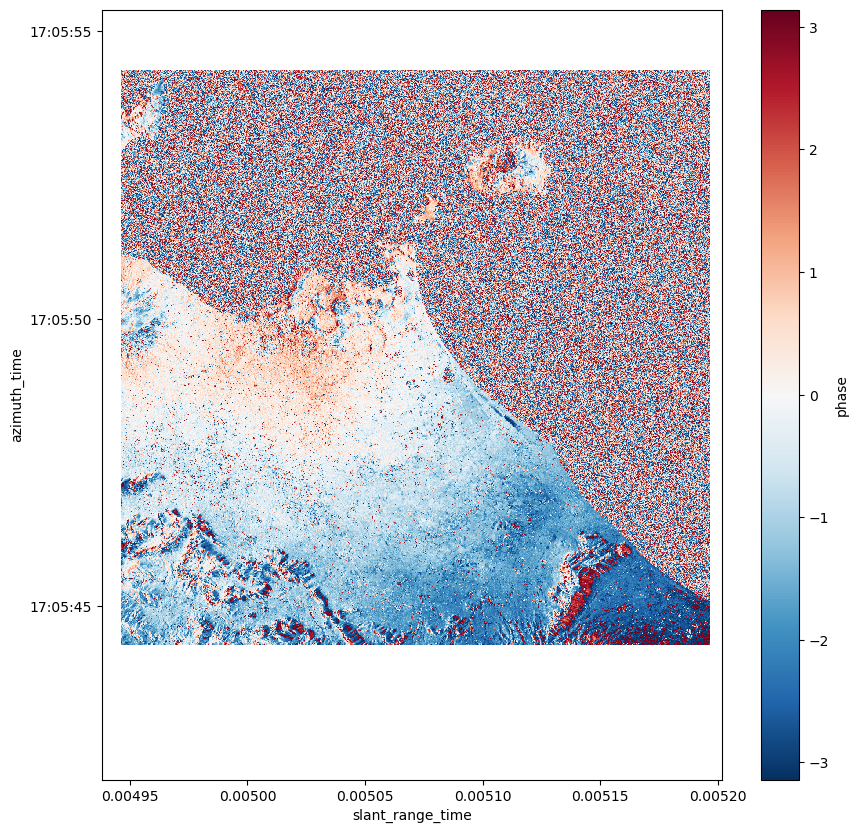
\includegraphics[width=0.45\linewidth]{Figures/mlc/DSC_S4/2025-01-14_2015-01-30_emi.png}
        \caption{The interferometric phase for the pair 2025-01-14 / 2025-01-30. Left: from the progressive interferometric phase estimation, right: from the EMI (full-covariance) estimation.}
    \label{fig:interf_pipe_emi}
\end{figure}

\begin{figure}[htb!]
    \centering
    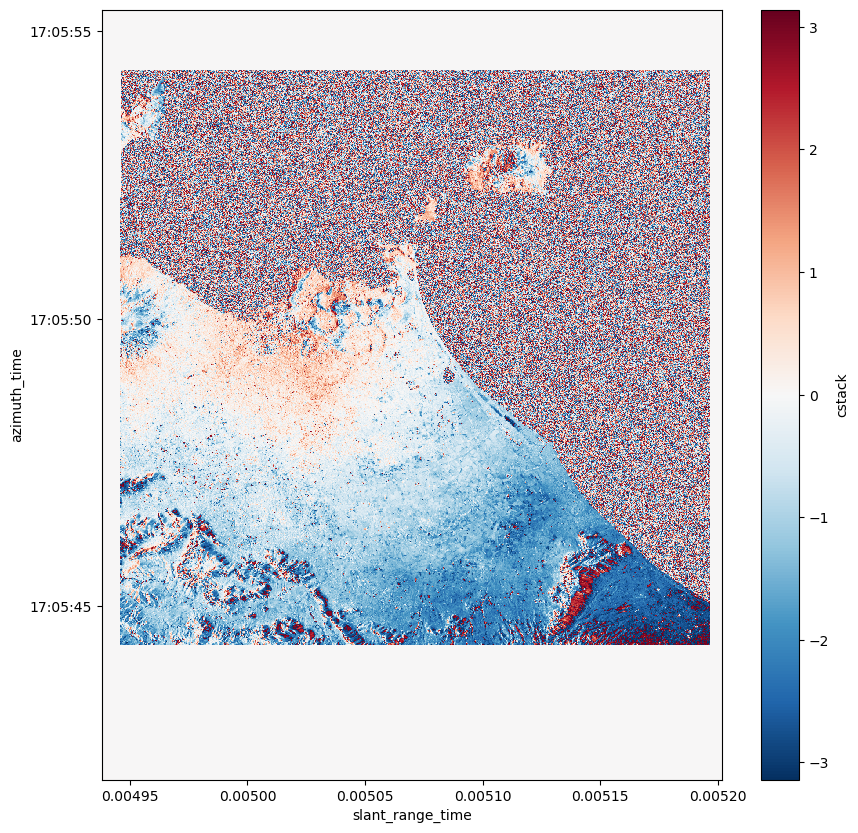
\includegraphics[width=0.45\linewidth]{Figures/mlc/DSC_S4/2025-01-14_2015-01-30_direct.png}
    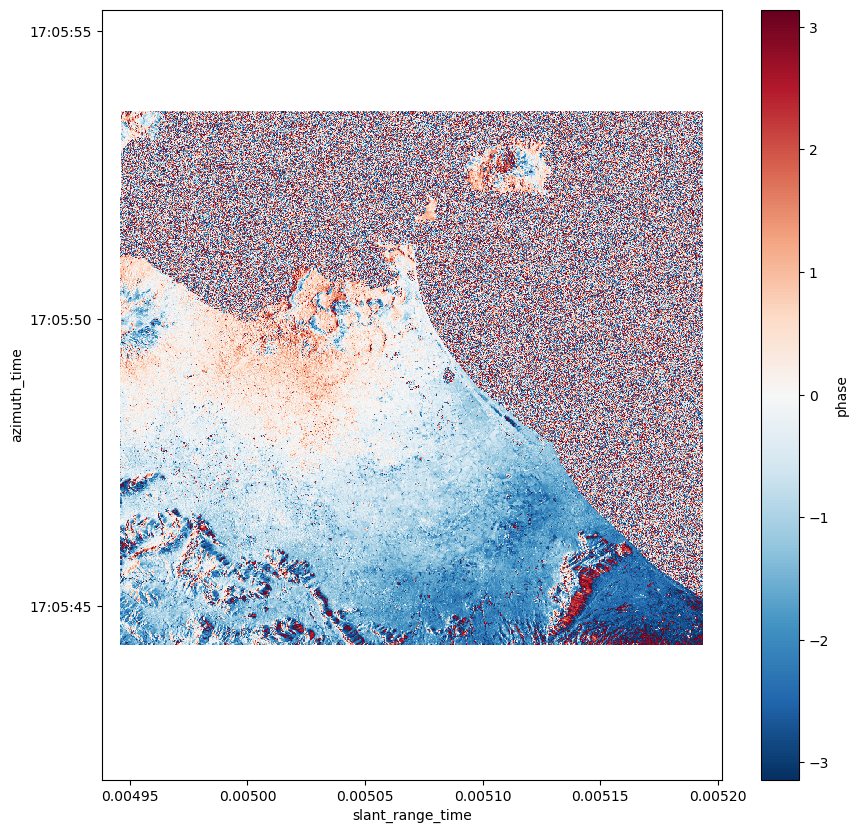
\includegraphics[width=0.45\linewidth]{Figures/mlc/DSC_S4/2025-01-14_2015-01-30_ndc.png}
        \caption{The interferometric phase for the pair 2025-01-14 / 2025-01-30. Left: from the direct interferogram, right: from the progressive phase estimation with fast-fading memory and without any drift control.}
    \label{fig:interf_direct_ndc}
\end{figure}


Checking the performance against a full-covariance method allows us to see that what we are producing has similar performance to state-of-the-art methods, despite being computationally cheaper. Checking the performance against direct interferograms allows us to quantify the long-term deformation bias: since this is expected to be negligible in the direct interferograms with a separation of months or years, the quantification shows practically the absolute deformation bias of our algorithm. The last comparison is going to show us the importance of controlling the phase drift; it is not helping validate the algorithm like the other two points.

Figures~\ref{fig:interf_pipe_emi} and~\ref{fig:interf_direct_ndc} show an example of the four products we are going to compare for a single interferometric pair.

The comparison of the results coming from different estimators is performed with complex exponentials to avoid unwrapping issues. Only at this point do we compute the phase and average it over the scene. For example, here is how we compute the phase difference $\phi_{diff}$ from $\phi_{PIPE}$ and $\phi_{EMI}$:
\begin{equation}
    \phi_{diff} = \angle e^{j(\phi_{PIPE} - \phi_{EMI})}.
\end{equation}



\begin{figure}[ht!]
    \centering
    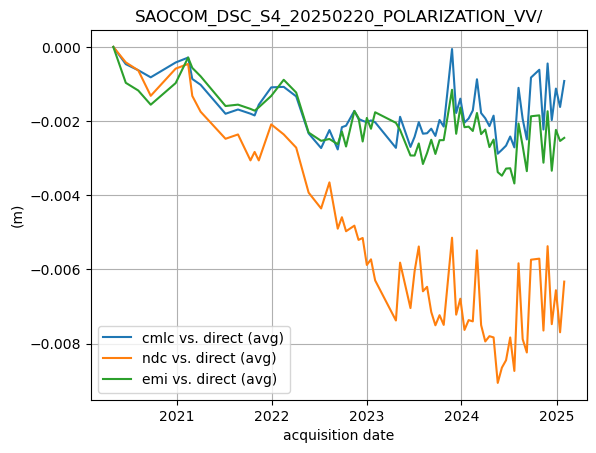
\includegraphics[width=0.8\linewidth]{Figures/mlc/DSC_S4/bias_mem_0.95_past_1.0_ma_0.0_mini_10.png}
    \caption{Deformation bias over time w.r.t. direct interferogram for different phase estimators.}
    \label{fig:bias_direct}
\end{figure}

We are going to analyze the evolution of the phase (or deformation) bias over time. The plot in Fig.~\ref{fig:bias_direct} shows the average displacement difference with respect to the direct interferogram, for points which have a coherence between 0.2 and 0.6 in the direct interferogram. The behavior of PIPE and EMI is very similar. Removing the drift control, i.e. the reference phase calibration step in the PIPE algorithm, introduces a drift of a couple of mm per year. EMI and PIPE exhibit some initial drift too, but this is smaller. The displacement error should become stable in the presence of long-term coherence.

All estimators are affected by a seasonal oscillation, which is likely related to vegetation or soil moisture content.

This analysis is limited by the need for a residual coherence in the direct interferogram. This might explain why the drift seems to stop after 4-5 years.

For this reason, we are also examining the evolution bias with respect to the EMI results. We are going to accumulate the differences at each time step and filter with the short-term coherence as estimated by the PIPE algorithm: this way, targets which are incoherent in the long run are not excluded as in the previous analysis. The plots reported in Fig.~\ref{fig:bias_emi} show that without drift control the drift is about 10 mm / year, whereas for our algorithm the drift appears to stop after reaching an initial value of around 5 mm. Some improvements could limit this initial bias accumulation, which is likely a warm-up effect.

\begin{figure}[htb!]
    \centering
    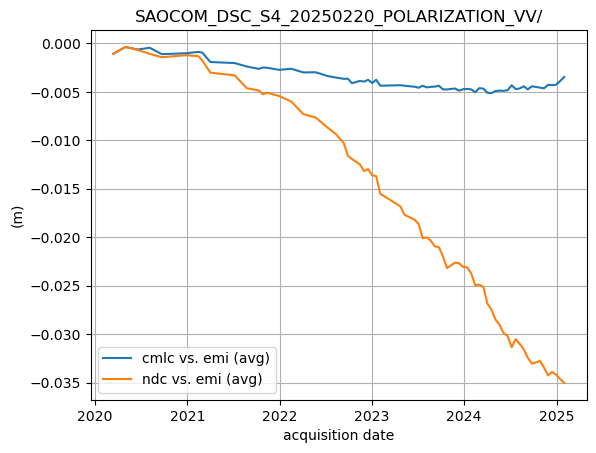
\includegraphics[width=0.8\linewidth]{Figures/mlc/DSC_S4/s1_mem_0.95_past_1.0_ma_0.0_mini_10.png}
    \caption{Deformation bias over time w.r.t. EMI interferogram for different phase estimators, reconstructed from lag-1 interferograms.}
    \label{fig:bias_emi}
\end{figure}


\subsubsection{Analysis of phase standard deviation over time}
The same analysis can be repeated for the standard deviation: the results are reported in Fig.~\ref{fig:std_direct}. In this case, the performance of EMI and PIPE is different. For short temporal intervals, PIPE has a smaller deviation; after two to three years, they are both very similar.

\begin{figure}[htb!]
    \centering
    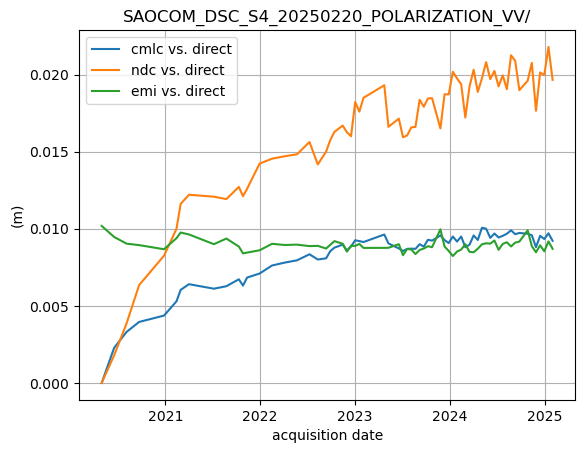
\includegraphics[width=0.8\linewidth]{Figures/mlc/DSC_S4/std_mem_0.95_past_1.0_ma_0.0_mini_10.png}
    \caption{Deformation standard deviation over time w.r.t. direct interferogram for different phase estimators.}
    \label{fig:std_direct}
\end{figure}


%\hl{Do we want to also add the performance having the reference in the middle of the stack?}


\subsection{Relative performance assessment (Sentinel-1)}
This section reports the results of the same analysis applied to the Sentinel-1 case.


\subsubsection{Analysis of phase bias over time}
Figure~\ref{fig:bias_direct_S1} and ~\ref{fig:bias_emi_S1} show the bias over time for a Sentinel-1 case (dataset 124) both w.r.t. the direct interferograms and w.r.t EMI. The observed behaviour is roughly similar but C-band appears to be more susceptible to bias even if the total period is much smaller.

\begin{figure}[ht!]
    \centering
    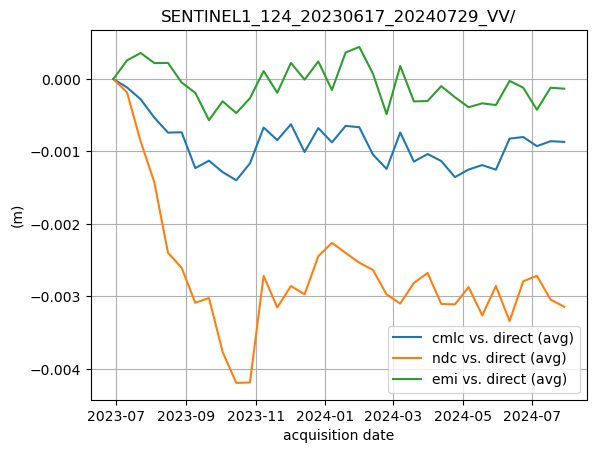
\includegraphics[width=0.8\linewidth]{Figures/mlc/S1_124/S1_124_bias_0.98_1.0_0.0.png}
    \caption{Deformation bias over time w.r.t. direct interferogram for different phase estimators.}
    \label{fig:bias_direct_S1}
\end{figure}

\begin{figure}[htb!]
    \centering
    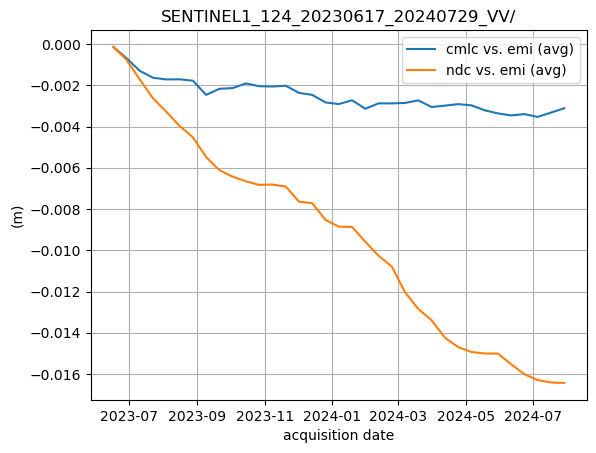
\includegraphics[width=0.8\linewidth]{Figures/mlc/S1_124/S1_124_s1_bias_0.98_1.0_0.0.png}
    \caption{Deformation bias over time w.r.t. EMI interferogram for different phase estimators, reconstructed from lag-1 interferograms.}
    \label{fig:bias_emi_S1}
\end{figure}


\subsubsection{Analysis of phase standard deviation over time}
A similar conclusion holds also for the standard deviation measured w.r.t. the direct interferogram (see Fig.~\ref{fig:std_direct_S1}): the behavior is similar between C and L-band, but the discrepancy between the proposed algorithm and EMI is a bit larger. This might have to do with the choice of parameters for the processing (e.g. the auto-regressive coefficient for the running reference).

\begin{figure}[htb!]
    \centering
    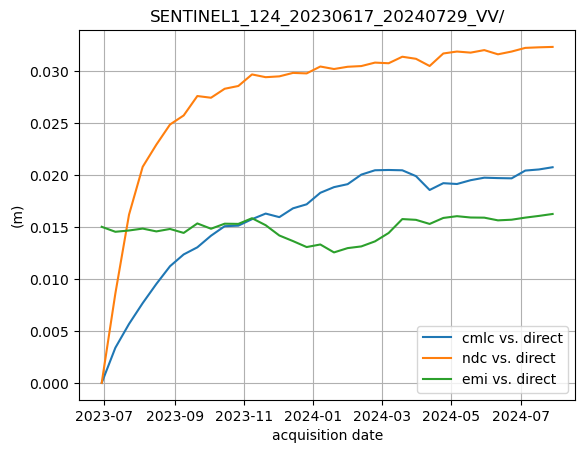
\includegraphics[width=0.8\linewidth]{Figures/mlc/S1_124/S1_124_std_0.98_1.0_0.0.png}
    \caption{Deformation standard deviation over time w.r.t. direct interferogram for different phase estimators.}
    \label{fig:std_direct_S1}
\end{figure}







\subsection{Theoretical models}
\label{sec:cmlc_models}
To assess the performance in an absolute sense, we resort to simulated data for which we know the desired output phase. 

We model the coherence over time as a stationary process with the following function of time:
\begin{equation}
    \gamma(t) = \gamma_1 e^{-|t|/t_1 -j \omega_1 t } + \gamma_2 e^{-|t|/t_2 -j \omega_2 t } + \gamma_3 e^{-|t|/t_3 -j \omega_3 t },
\end{equation}
for  $t \neq 0$ (and $\gamma(0)=1$), with the following values for the parameters:
\begin{equation}
    \begin{matrix}
    \gamma_1 = 0.18 &   t_1 = 11 \, \mathrm{days} &  \omega_1 = 0.030 \, \mathrm{rad/day}\\
    \gamma_2 = 0.25& t_2 = 50 \, \mathrm{days} & \omega_2 = 0.002  \, \mathrm{rad/day}\\
    \gamma_3 = 0.13 &  t_3 = \infty \, \mathrm{days} & \omega_3 = 0.000  \, \mathrm{rad/day} \\
    \end{matrix} 
    \nonumber
\end{equation}
This parametrization ensures the presence of non-zero closure phases, which have the potential to generate a bias in the estimated phases and thus deformation drifts, especially when integrating short-term multilooked phases. The first two terms represent targets which are both decorrelating and rotating, f.i. because of an accumulation of biomass; the third target is not decorrelating. Values are taken from a previous study of Sentinel-1 data. A precise correspondence to reality is anyway not crucial for the verification of the algorithm.

We then performed 1000 Monte-Carlo simulations for 8 years of acquisitions with a repeat pass of 16 days and according to the coherence model described above. For each acquisition, we generated 200 independent samples (looks). Finally, we applied both the EMI and PIPE estimators to the synthetic data.

Figure~\ref{fig:bias_synth} shows the phase bias as a function of time for both estimators. The EMI results show a very small bias, which confirms that EMI is a good estimator provided that there is a long-term coherence contribution.
The PIPE results show an initial bias build-up but, after 1-2 years, there is no permanent drift in the estimated deformation.

\begin{figure}[htb!]
    \centering
    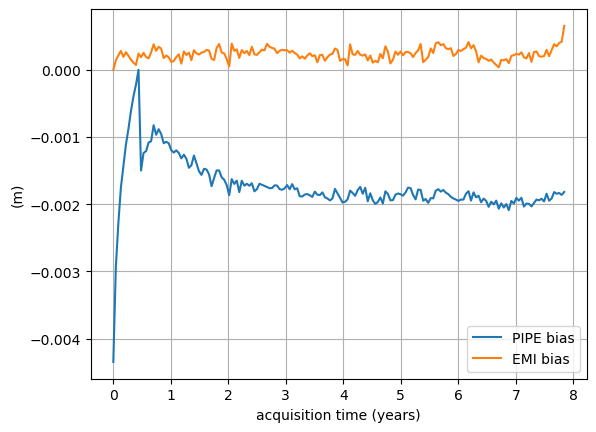
\includegraphics[width=0.48\linewidth]{Figures/mlc/PIPE_Synthetic/PIPE_bias_EMI_bias.png}
    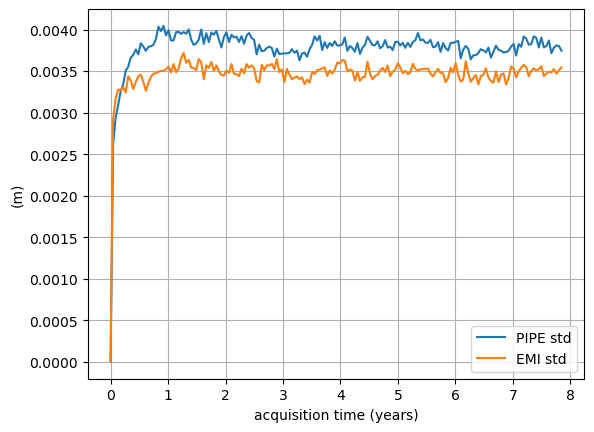
\includegraphics[width=0.48\linewidth]{Figures/mlc/PIPE_Synthetic/PIPE_std_EMI_std.png}
    \caption{Deformation bias (left) and standard deviation (right) over time for EMI and PIPE phase estimators.}
    \label{fig:bias_synth}
\end{figure}


\subsubsection{Internal coherence modelling}
The PIPE algorithm computes two important interferograms: one is the interferogram between the running reference and the new incoming acquisition (which is the basis for the phase product itself); the other is the interferogram between the running reference and a past reference, which is necessary to keep the phase drift under control (see Fig.~\ref{fig:internal_coherence_cartoon}). Knowing the ``true'' coherence between any two acquisitions makes it possible to predict those two coherence values, which we can then compare with the observed values to verify the internal working of the algorithm.

\begin{figure}[htb!]
    \centering
    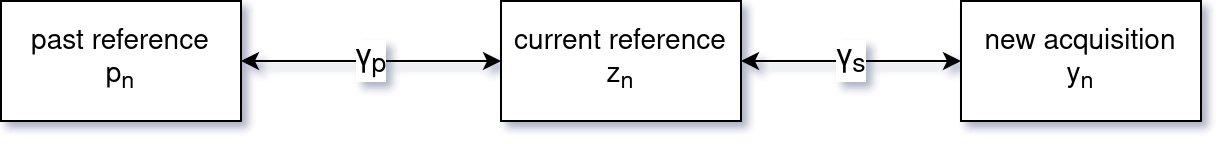
\includegraphics[width=0.8\linewidth]{Figures/mlc/PIPE_Synthetic/Two_coherences.drawio.png}
    \caption{Two coherence values are computed inside the PIPE algorithm, one is the short-term coherence between the running reference and the incoming acquisition, the other is between the running reference and the past reference to calibrate the phase of the running reference.}
    \label{fig:internal_coherence_cartoon}
\end{figure}

Both past and running references are really just linear combinations of the original acquisitions. Knowing the weights from the parameters chosen for the PIPE algorithm, and assuming perfect phase reconstruction, we can derive the said coherence. In general, if $y'$ and $y''$ are two linear combinations of the original acquisitions $y_i$, such as:
\begin{align}
y' &= \sum_i w_i' \, y_i \\
y'' &= \sum_i w_i''\,  y_i, \\
\end{align}
the correlation is
\begin{equation}
    \mathrm{corr}(y', y'')= \sum_{i,j} w_i' w_j'' \, \gamma(y_i, y_j).
\end{equation}
Finally, the coherence is going to be:
\begin{equation}
    \gamma(y', y'') = \frac{\mathrm{corr}(y', y'')}{\sqrt{\mathrm{corr}(y', y') \ \mathrm{corr}(y'', y'')}}.
\end{equation}
In particular, the running reference $z_{n+1}$ can be written explicitly (and approximately) as
\begin{equation}
    z_{n+1} = y_n + \alpha\,y_{n-1} + \alpha^2\,y_{n-2} + \cdots,
    \label{eqn:running_linear}
\end{equation}
and therefore $1, \, \alpha, \, \alpha^2\, \cdots$ are the weights to be considered in the equations above.

Figure~\ref{fig:internal_coherence} shows the evolution of the coherence for the two interferograms, which are computed inside the PIPE algorithm and the theoretical values derived from the formulas described here. After an initial transition, which we have not modeled, it appears that the coherence settles close to the expected values, confirming the inner workings of the algorithm.

\begin{figure}[htb!]
    \centering
    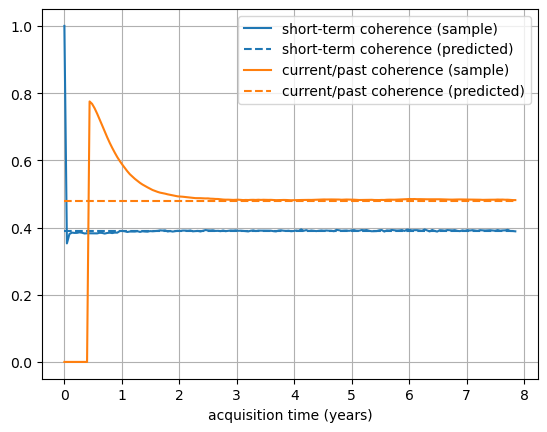
\includegraphics[width=0.8\linewidth]{Figures/mlc/PIPE_Synthetic/coherences_predicted_vs_sampled.png}
    \caption{Predicted vs. sampled coherence for the two internal interferograms computed in the PIPE algorithm.}
    \label{fig:internal_coherence}
\end{figure}

The ultimate goal of this analysis was to derive the standard deviation of the estimated phase from the coherence levels. Unfortunately, the results do not show a level of match with the simulations sufficient for this kind of theoretical analysis. In the analysis, we have not modeled the uncertainty in the phases that enter the linear combination of the acquisition (e.g. in Eq.~\ref{eqn:running_linear} ). It seems that this kind of approximation is sufficient to estimate properly the average coherence (where the error intervenes as a second order term) but not the phase uncertainty itself (where the error intervenes directly). Further attempts in this direction were not sufficient for a satisfactory theoretical modeling.

\subsection{Computational performance}
\label{sec:cmlc_computation}

The computational performance of the phase-estimation algorithm proposed here is very high (i.e. the algorithm is very efficient). The cost is only a few complex multiplications for each pixel, and for each new incoming acquisition. A full-covariance matrix approach would have a cost that grows quadratically with the number of acquisitions and would require the simultaneous access to the entire acquisition history, at least for the multi-looking window.

At the moment it looks like the most expensive step is the geocoding from \acs{cmlc} to \acs{gmlc}. This cost is comparable to the one for generating \acs{nrb} products but could be reduced by adopting a simpler geocoding strategy.

\subsection{Criticalities and weakness}
\label{sec:cmlc_criticalities}

The performance study has shown that there is a needed warm-up period in which the phase is drifting. If this is not acceptable, it is necessary to delay the delivery of the product so that the bias can be corrected, for example, with the application of a full-covariance matrix estimator.

The sampling of the phase signal is not optimal as it is performed in the demonstration software. Since the final product should be sampled on a 50 m grid, the underlying multi-looking should be performed on an area larger than $(50 \mathrm{m})^2$. Otherwise, there is a risk of frequency aliasing (actually, this is not limited to phase products).

After that, resampling to UTM grid should pose no major problem since the signal is already properly sampled at the \acs{cmlc} level.

%\section{Enhanced NRB \& ORB (ENRB \& EORB)}
\label{sec:enh}

\subsection{Evaluation criteria}
\label{sec:enh_criteria}

The evaluation criteria for \acs{enrb} and \acs{eorb} are the same as for the \acs{nrb} and \acs{orb} products, since the underlying radiometric, geometric, and statistical properties are preserved. The additional sidelobe suppression or ghost removal improves visual quality and noise characteristics but does not alter the fundamental assessment dimensions, such as radiometric consistency, slope-effect removal, \acs{dem} and orbital dependencies, or the statistical stability of $\sigma_0$ values. Therefore, \acs{enrb}/\acs{eorb} inherit the same evaluation framework and quality benchmarks as their parent \acs{nrb}/\acs{orb} products.

\subsection{Theoretical models}
\label{sec:enh_models}

The \acs{enrb}/\acs{eorb} products' theoretical models to evaluate performances are directly inherited from the \acs{nrb} and \acs{orb} products, as their generation is based on the same processing principles. Any performance assessment therefore follows the same criteria and methodologies.

\subsection{Computational performance}
\label{sec:enh_computation}

The computational performance of \acs{enrb} and \acs{eorb} directly follows that of the \acs{nrb} and \acs{orb} products. Since their generation relies on the same processing chain, including rasterization, shadow masking, and possible stack-based co-registration, the overall cost is essentially inherited. The only additional burden comes from sidelobe suppression or ghost removal, which is marginal compared to the dominant steps already present in \acs{nrb}/\acs{orb} processing. Therefore, \acs{enrb}/\acs{eorb} maintain the same scalability and efficiency characteristics as their parent products.

\subsection{Criticalities and weakness}
\label{sec:enh_criticalities}
For \acs{enrb} products, the same criticalities and weaknesses described for \acs{nrb} apply. Since \acs{enrb} products are derived directly from \acs{nrb}, their performance is equally dependent on the accuracy of orbital data, \acs{dem} quality, and timing corrections. The main difference lies in the application of filtering techniques (ghost removal and sidelobe suppression), which may slightly mitigate noise but do not alter the fundamental dependencies of the product.

For \acs{eorb} products, the situation mirrors that of \acs{orb}. The reliability of the output is still determined by the quality of the input \acs{enrb} data, wind fields, and the geophysical model function, while the filtering step has only a marginal effect. Therefore, the same considerations regarding reference wind choice and angle of incidence compensation remain valid.


\section{Geoprojected Ground Motion (GGM)}
\label{sec:ggm}

\subsection{Evaluation criteria}
\label{sec:ggm_criteria}

The evaluation of \acs{ggm} products is based on the relationship between the the input and output noise levels. The core idea is to evaluate how the spatial aggregation and inversion steps propagate or attenuate the noise present in the original \acs{gpro}/\acs{gpao} measurements. By estimating the expected noise in the output vectors as a function of the input noise characteristics and the resolution of the grid, the quality of the \acs{ggm} output can be quantitatively evaluated.

\subsection{Theoretical models}
\label{sec:ggm_models}
To retrieve the 3D surface displacement \(\mathbf{d} = [\textbf{d}^e, \textbf{d}^n, \textbf{d}^u]^\top\) (east, north, up), we consider four measurements:

\begin{itemize}
    \item \(\textbf{rg}_{\text{A}}\): range offset from ascending acquisition,
    \item \(\textbf{rg}_{\text{D}}\): range offset from descending acquisition,
    \item \(\textbf{az}_{\text{A}}\): azimuth offset from ascending acquisition,
    \item \(\textbf{az}_{\text{D}}\): azimuth offset from descending acquisition.
\end{itemize}

Each measurement can be expressed as a linear projection of the 3D displacement vector:

\[
\mathbf{d} = \mathbf{A} \mathbf{u}
\]

where \(\mathbf{d} \in \mathbb{R}^4\) is the measurement vector:

\[
\mathbf{d} =
\begin{bmatrix}
\textbf{rg}_{\text{A}} \\
\textbf{rg}_{\text{D}} \\
\textbf{az}_{\text{A}} \\
\textbf{az}_{\text{D}}
\end{bmatrix}
\]

and \(\mathbf{A} \in \mathcal{M}(4, 3, \mathbb{R})\) is the design matrix composed of the unit vectors projecting the 3D motion into each measurement geometry. For example:

\[
\mathbf{A} =
\begin{bmatrix}
\textbf{los}^{e}_{\text{A}} & \textbf{los}^{n}_{\text{A}} & \textbf{los}^{u}_{\text{A}} \\
\textbf{los}^{e}_{\text{D}} & \textbf{los}^{n}_{\text{D}} & \textbf{los}^{u}_{\text{D}} \\
\textbf{lof}^{e}_{\text{A}} & \textbf{lof}^{n}_{\text{A}} & \textbf{lof}^{u}_{\text{A}} \\
\textbf{lof}^{e}_{\text{D}} & \textbf{lof}^{n}_{\text{D}} & \textbf{lof}^{u}_{\text{D}} \\
\end{bmatrix}
\]

To estimate \(\mathbf{u}\), we solve the overdetermined system using the \acs{lmse} approach:

\[
\hat{\mathbf{u}} = (\mathbf{A}^\top \mathbf{A})^{-1} \mathbf{A}^\top \mathbf{d}
\]

\begin{figure}[h!]
\centering
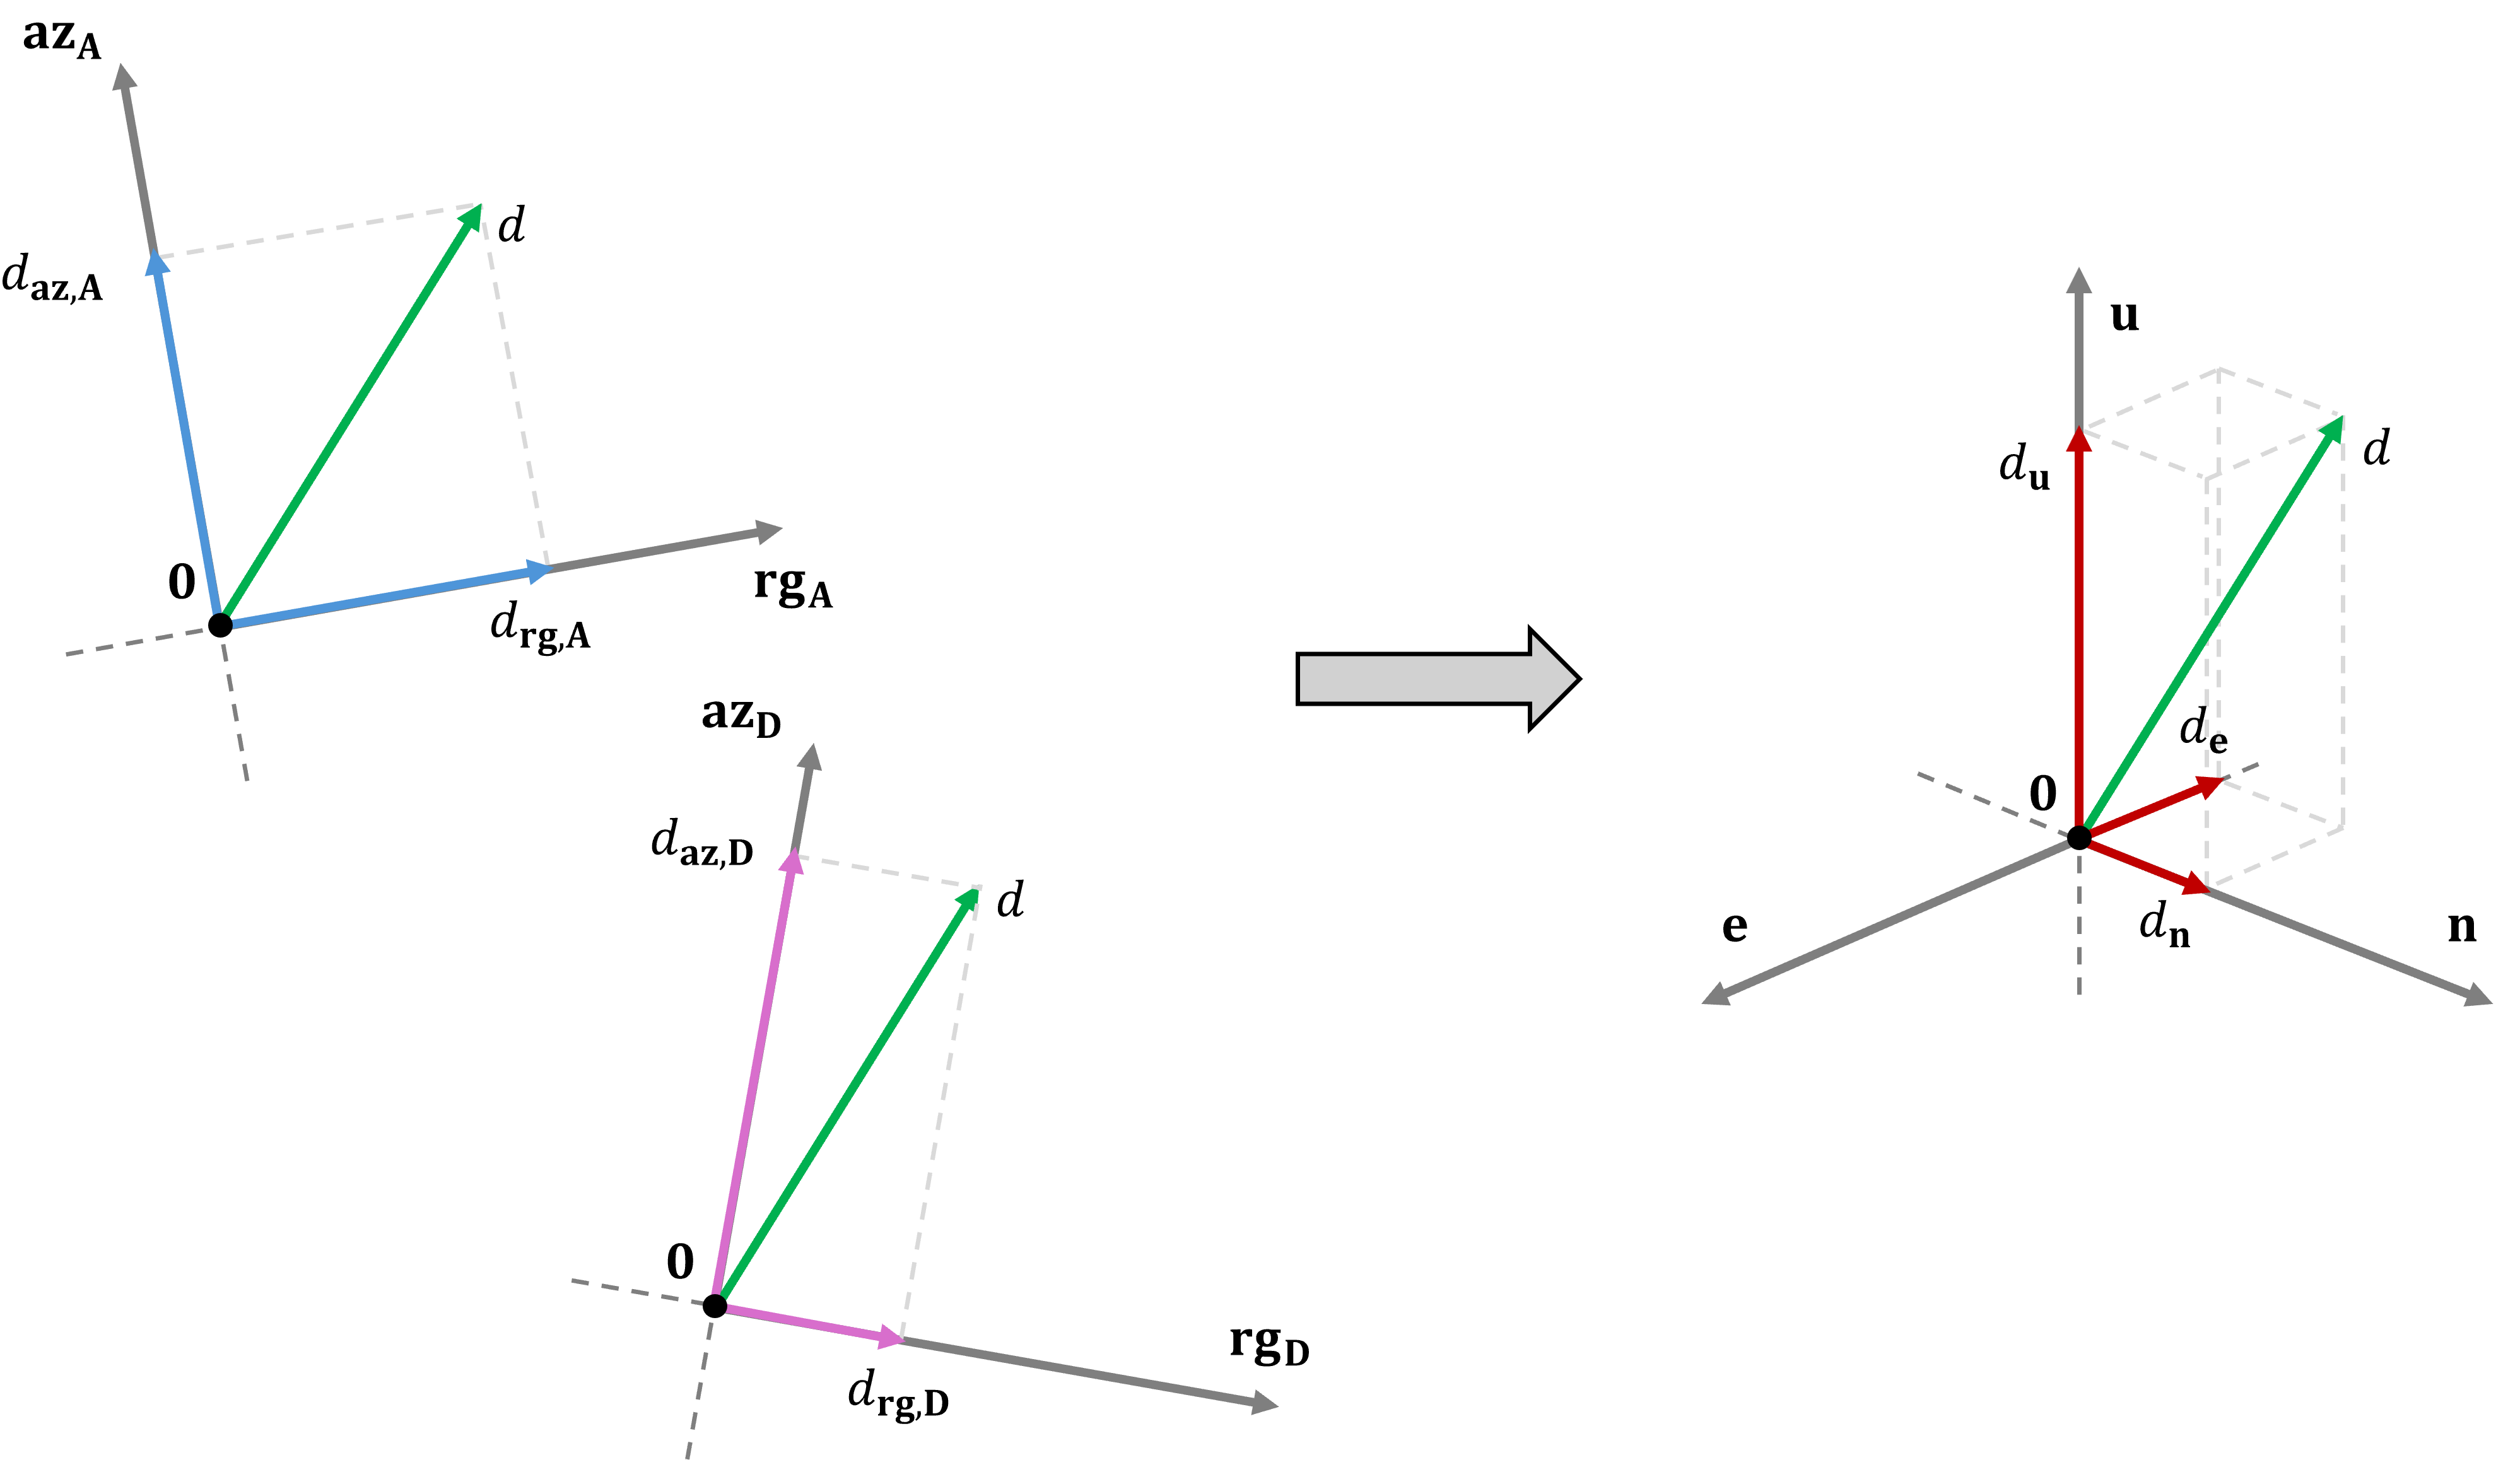
\includegraphics[width=15.0cm]{Figures/ggm/ggm_scheme.png}
\caption{Simple graphic scheme for the generation of the \acs{ggm} products starting from the \acs{pro}/\acs{pao} products.}
\end{figure}

If the measurement noise is not uniform, a weighted \acs{lmse} solution is more appropriate:

\[
\hat{\mathbf{u}} = (\mathbf{A}^\top \mathbf{W} \mathbf{A})^{-1} \mathbf{A}^\top \mathbf{W} \mathbf{d} = \mathbf{L} \mathbf{d}
\]

where \(\mathbf{W}\) is a diagonal weight matrix, typically set as the inverse variance of the measurements:

\[
\mathbf{W} = \operatorname{diag} \left( \sigma_{\text{A}, rg}^2, \sigma_{\text{D}, rg}^2, \sigma_{\text{A}, az}^2, \sigma_{\text{D}, az}^2 \right) ^ {-1}
\]

with \(\sigma_r\) and \(\sigma_a\) representing the standard deviations of range and azimuth offsets, respectively, and \( \mathbf{L} = (\mathbf{A}^\top \mathbf{W} \mathbf{A})^{-1} \mathbf{A}^\top \mathbf{W} \).

Given the significantly different noise levels associated with azimuth and range offsets in \acs{s1} and \acs{rosel} data, it is critical to account for these discrepancies when assessing or improving the accuracy of derived ground motion products: the azimuth offset accuracy is indeed one or two orders of magnitude worse than the range offset accuracy. To mitigate the high noise in azimuth offsets and enhance the reliability of azimuth-constrained products, it is advisable to spatially coarsen the azimuth resolution (for instance, through multilook). This spatial aggregation can reduce the effective noise level, depending on the size of the averaging window. 

\subsection{Computational complexity}
\label{sec:ggm_computation}

The generation of \acs{ggm} products from \acs{gpro}/\acs{gpao} input products follows a three-steps process:

\begin{itemize}
    \item \acs{gpao} products typically exhibit significantly lower resolution in the azimuth direction compared to GPRO products. To mitigate this and ensure more balanced noise characteristics, a uniform filter is applied to GPAO measurements. This filtering step ensures that the resulting noise levels become comparable to those of full-resolution \acs{gpro} data.

    \item The geographical coverage of the input \acs{gpro}/\acs{gpao} products is analyzed to determine their spatial extent. A regular metric grid is then defined to cover the intersection area of the inputs. The resolution of this grid is chosen based on the desired spatial granularity and serves as an implicit estimate of the input (and consequently output) noise level. Within each grid cell, all input data points that fall inside the cell are aggregated, typically through an arithmetic averaging process. This spatial averaging helps to reduce noise and prepare the data for the inversion step. The corresponding \acs{los}/\acs{lof} vectors are averaged in the same way.

    \item For each populated grid cell, a linear system of equations of size \( 4 \times 3 \) is constructed using the averaged input data. This system is then solved using a linear \acs{lmse} approach to estimate the 3-dimensional output vector (North-South, East-West, Vertical) for each cell. This inversion is performed independently for each grid cell. Further details are provided in \ref{sec:ggm_models}.
\end{itemize}

Let \( M \) and \( N \) denote, respectively, the maximum acquisition length (in azimuth pixels) and the maximum swath width (in range pixels) for all input products (without loss of generality, we assume that for each input product, the azimuth dimension is at most \( M \) pixels and the range dimension is at most \( N \) pixels).

The complexity of the preprocessing step is linear in the number of input pixels (\( \mathcal{O}(M \times N) \)), since the uniform filter is applied with constant cost per pixel.

The number of output grid cells, denoted \( N_C \), is also proportional to \( M \times N \). Both the averaging step and the linear inversion step are applied once per output cell: since the inversion involves solving a fixed-size (\( 4 \times 3 \)) linear system and the number of input measurements per cell is limited by the grid resolution, the per-cell cost is constant. Therefore, the complexity of both steps is also \( \mathcal{O}(N_C) = \mathcal{O}(M \times N) \).

In conclusion, the total computational complexity of the entire process is linear in the number of input image pixels:
\[
C_{\text{tot}} = \mathcal{O}(M \times N)
\]

\subsection{Criticalities and weakness}
\label{sec:ggm_criticalities}

The \acs{ggm} products inherit all the intrinsic limitations and potential inaccuracies of their input data, the \acs{gpro} and \acs{gpao} products. Any systematic errors, noise characteristics, or biases present in the input measurements or their respective processing pipelines will propagate into the final \acs{ggm} outputs.

An additional critical aspect arises from the anisotropic resolution of the input data, particularly in the case of \acs{gpao} products: these products typically exhibit significantly heigher noise with respect to \acs{gpro} products. If left unaddressed, this anisotropy can lead to numerical instability or ill-posedness in the per-cell linear inversion step, as the underlying linear systems may become sensitive to directional noise and lack robustness. To mitigate this issue, a uniform spatial filtering operation is applied as a preprocessing step to \acs{gpao} measurements. This step is crucial to homogenize the noise characteristics across all input products, thereby improving the conditioning of the inversion systems. However, this comes at the cost of reduced spatial resolution for \acs{gpao} products, and may result in some loss of local detail in the final \acs{ggm} output.

In summary, while the preprocessing step is essential to ensure numerical stability and consistent noise behavior in the inversion process, it also represents a trade-off between robustness and spatial fidelity. These factors, together with inherited input limitations, must be carefully considered when interpreting or applying \acs{ggm} products.



\section{Stripmap equivalent CSLC}
\label{sec:stripeq}

\subsection{Evaluation criteria}
\label{sec:stripeq_criteria}

The Stripmap-equivalent \acs{stripeq} \acs{cslc} image is a full-resolution \acs{sar} image (matching the resolution of the input) that combines multiple bursts from wide-area acquisition modes, such as Terrain Observation by Progressive Scans SAR (\acs{topsar}) or ScanSAR, to produce one seamless image with the spatial consistency and phase integrity of \acs{sm} mode.

Managing SAR acquisitions in burst mode is inherently more complex than conventional \acs{sm} acquisitions. The (\acs{stripeq}) product has been devised to hide this complexity from downstream processors, enabling burst-mode data to be ingested by existing Stripmap oriented processing chains without modification. Therefore, the \acs{stripeq} product must remain fully compatible with standard amplitude and phase-based workflows, including radiometric image generation, interferogram formation, and coherence estimation.

Burst-based acquisition modes impose an additional, azimuth-dependent phase modulation because the antenna beam is continuously steered during the synthetic aperture time. If left uncorrected, this modulation introduces phase discontinuities in the overlap regions between adjacent bursts, degrading interferometric coherence. Consequently, dedicated processing steps must be applied to ensure phase continuity and Doppler alignment before the bursts are coherently mosaicked. Therefore the chosen evaluation criteria for this product are indicators that measure (i) the phase continuity across former burst boundaries and (ii) the spatial homogeneity of coherence maps derived from co‑registered \acs{stripeq} image pairs. These metrics ensure that the final product meets the precision requirements for interferometric, change‑detection, and time‑series applications.

\subsection{Theoretical models}
\label{sec:stripeq_models}


Burst-mode acquisitions scanned in azimuth (\acs{topsar}, ScanSAR) introduce a deterministic, azimuth-dependent Doppler centroid $f_{DC}(\eta)$ due to the variation of the squint angle in the azimuth direction. This variation produces a pronounced phase modulation that can significantly degrade the quality of the resulting interferogram.

In ideal conditions—where master and slave images are perfectly co-registered in azimuth—the phase modulation cancels out during interferogram formation. However, in realistic scenarios, even a small residual co-registration error between the reference and slave images results in incomplete cancellation, leaving a residual phase ramp in each burst interferogram. The magnitude of this residual is directly related to the degree of misregistration. When such burst interferograms are mosaicked, phase discontinuities manifest at the burst overlap regions, as illustrated in Figure~\ref{fig:ESD_example}. This figure shows the phase mosaics obtained using the same master and two different slaves. The phase jumps are less visible in the left panel than in the right panel, due to the lower misregistration present in the left case compared to the right.

\begin{figure}[h!]
\centering
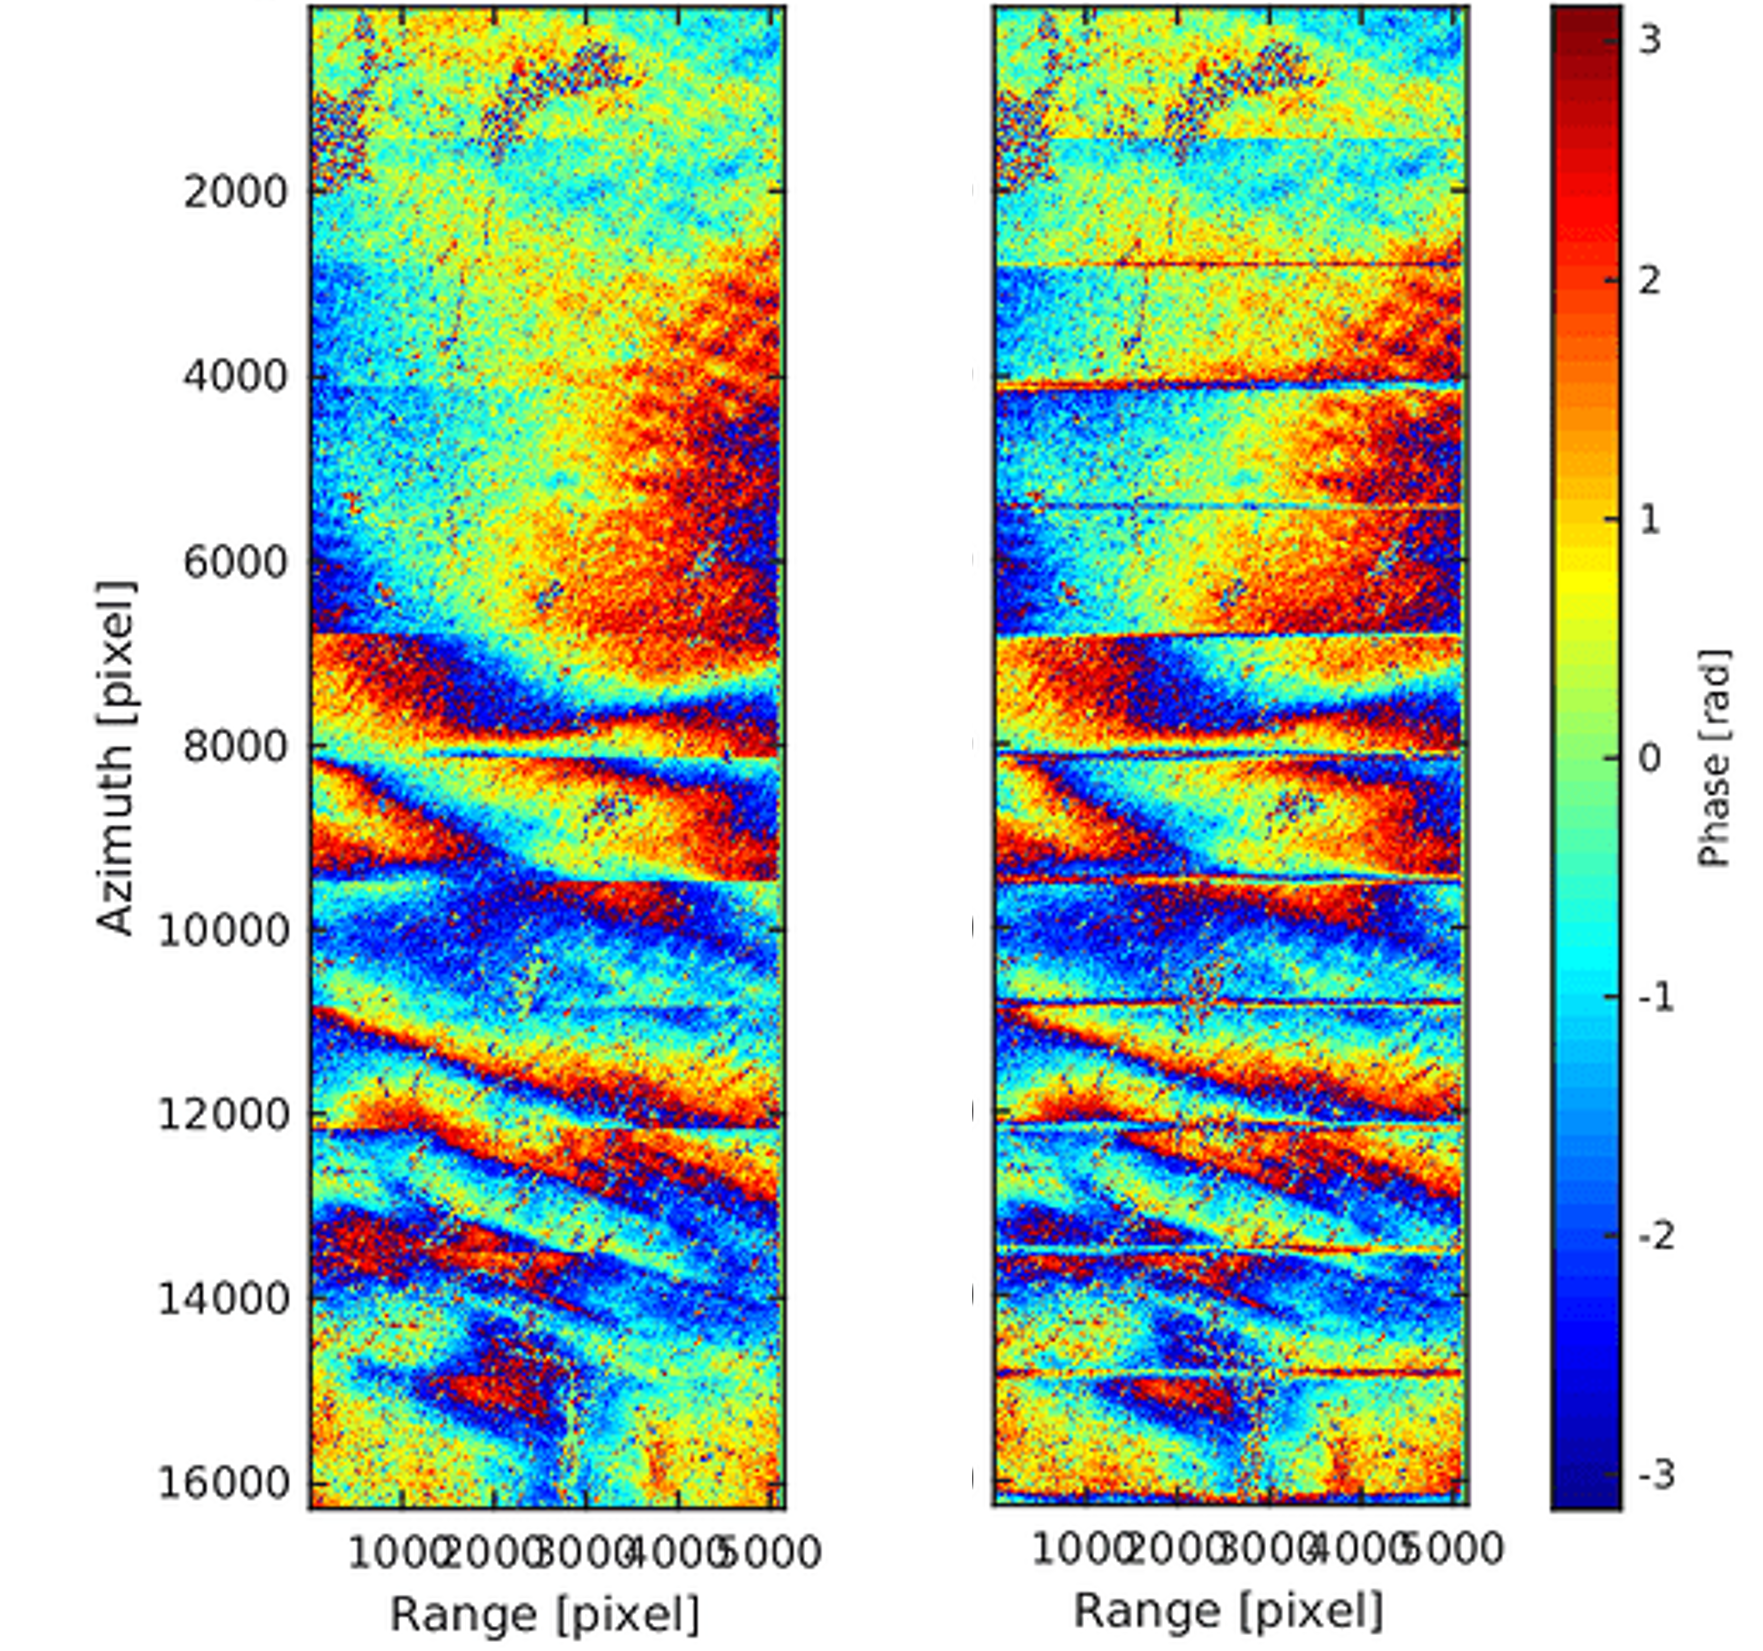
\includegraphics[width=0.9\textwidth]{Figures/strip_eq/ESD_example.png}
\caption{Interferometric phase mosaics derived from the same master image and two different slave acquisitions (\acs{s1} IW mode). The left panel exhibits smaller phase discontinuities across burst boundaries due to an higher accurate azimuth co-registration. In contrast, the right panel shows visible phase jumps resulting from increased residual misregistration, highlighting the critical need for sub-pixel accuracy in burst alignment for phase sensitive applications.}
\label{fig:ESD_example}
\end{figure}

More formally, using a small-angle approximation, a residual azimuth co-registration error of $\Delta t$ seconds introduces a phase ramp across the burst interferogram:

\begin{equation}
\Delta \phi_{az} = 2\pi \Delta f_{DC}\Delta t = \lambda \Delta \beta \Delta t
\label{eq:phase_jump}
\end{equation}

Here, $\Delta f_{DC}$ is the Doppler centroid variation, $\Delta \beta$ the corresponding change in squint angle, and $\Delta t$ the azimuth misregistration.

This relationship forms the basis for defining the accuracy requirements of azimuth co-registration to avoid phase jumps that could compromise the usability of \acs{stripeq} products for phase sensitive applications. For Sentinel-1, with a maximum $\Delta f_{DC}$ of approximately 5 kHz, limiting the phase ramp to 1/100 of a cycle (≈3.6°) requires a co-registration accuracy of about 0.001 pixels—equivalent to roughly 1.3 cm at the sensor's azimuth sampling rate.

Such stringent precision surpasses the capabilities of traditional methods like cross-correlation using small patches, where correlation peaks often provide only pixel level (or at most an accuracy of about 0.1 pixels) estimates. 

Considering the ROSE-L mission, the expected Doppler centroid variation is significantly lower than that of \acs{s1}. For \acs{rosel}, $\Delta f_{DC}$ is estimated to be approximately 1.4 kHz, resulting in a less stringent co-registration requirement in the azimuth direction. Nevertheless, if we still aim to limit the phase ramp to 1/100 of a cycle ($\approx 3.6°$), the required co-registration accuracy remains around 0.01 pixels-an order of magnitude more relaxed than in the \acs{s1} case, yet still beyond the capabilities of conventional co-registration methods based on standard cross-correlation.

Figure~\ref{fig:CRG_vs_FDC} illustrates the required co-registration accuracy (expressed in meters) as a function of $\Delta f_{DC}$, under different tolerances for allowable phase jumps between consecutive bursts. The two vertical dotted lines represent the \acs{s1} (red) and \acs{rosel} (yellow) configurations, based on the maximum $\Delta f_{DC}$ values anticipated for each SAR mission.

\begin{figure}[h!]
\centering
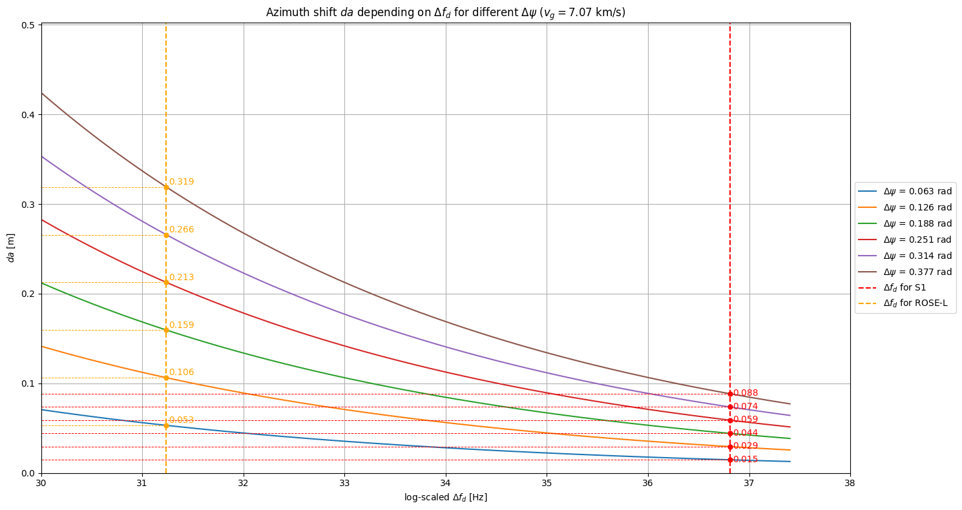
\includegraphics[width=0.9\textwidth]{Figures/strip_eq/CRG_accuracy_vs_fdc.png}
\caption{Required co-registration accuracy in meters as a function of Doppler centroid variation $\Delta f_{DC}$, under different thresholds of allowable phase jumps across burst boundaries. The red and yellow vertical lines correspond to \acs{s1} and \acs{rosel} mission parameters, respectively.}
\label{fig:CRG_vs_FDC}
\end{figure}

The previously discussed considerations highlight that to obtain a valid \acs{stripeq} \acs{ard} product, advanced techniques such as Spectral Diversity (SD) or Enhanced Spectral Diversity (ESD)—which analyse phase differences in burst overlap regions—must be employed.

The Spectral Diversity (SD) approach \citep{Scheiber2000} uses frequency shifts between azimuth looks, induced by the interferometric baseline, to estimate $\Delta t$ with sub-pixel accuracy by measuring phase differences in the azimuth sub-band cross-spectrum.

The Enhanced version of Spectral Diversity (\acs{esd}) \citep{Martínez2016} refines SD for \acs{topsar} mode. This method achieves empirical accuracies of approximately $10^{-4}$ pixels, comfortably within the Sentinel-1 requirement.

It must be highlighted that the requirement for the creation of a valid \acs{stripeq} \acs{ard} product also depends on the quality of the \acs{cslc} input data, from which consecutive bursts and subswaths are merged to create a Stripmap-like product. Once the previously described co-registration accuracy in the azimuth direction is met—by applying advanced refinement techniques such as SD and ESD—the deterministic phase ramp can be effectively removed. This enables consecutive bursts to be coherently mosaicked without introducing phase discontinuities, ensuring that the \acs{stripeq} product remains fully compatible with amplitude- and phase-based downstream applications.

Just for demonstration purposes, a test was conducted using a pair of Sentinel-1 \acs{iw} mode acquisitions over Greenland. Starting from \acs{cslc} products where individual bursts were preserved, the Enhanced Spectral Diversity (\acs{esd}) technique was applied to refine the azimuth co-registration between the master and slave images. Following this refinement, the bursts of both the master and the slave were independently mosaicked to generate two \acs{stripeq} products.

The resulting products were then used to compute a full-resolution interferogram and the corresponding interferometric coherence map. Figure~\ref{fig:interf_coh_maps} presents the results: the top panel shows the coherence map, while the bottom panel displays the interferometric phase. Both outputs exhibit seamless continuity across burst and subswath boundaries, confirming the preservation of phase integrity. The only notable effect is a slight increase in coherence when moving from the first to the second subswath. This is attributed to a higher oversampling factor in the second subswath, which leads to improved pixel-to-pixel correlation.

\begin{figure}[ht!]
\centering
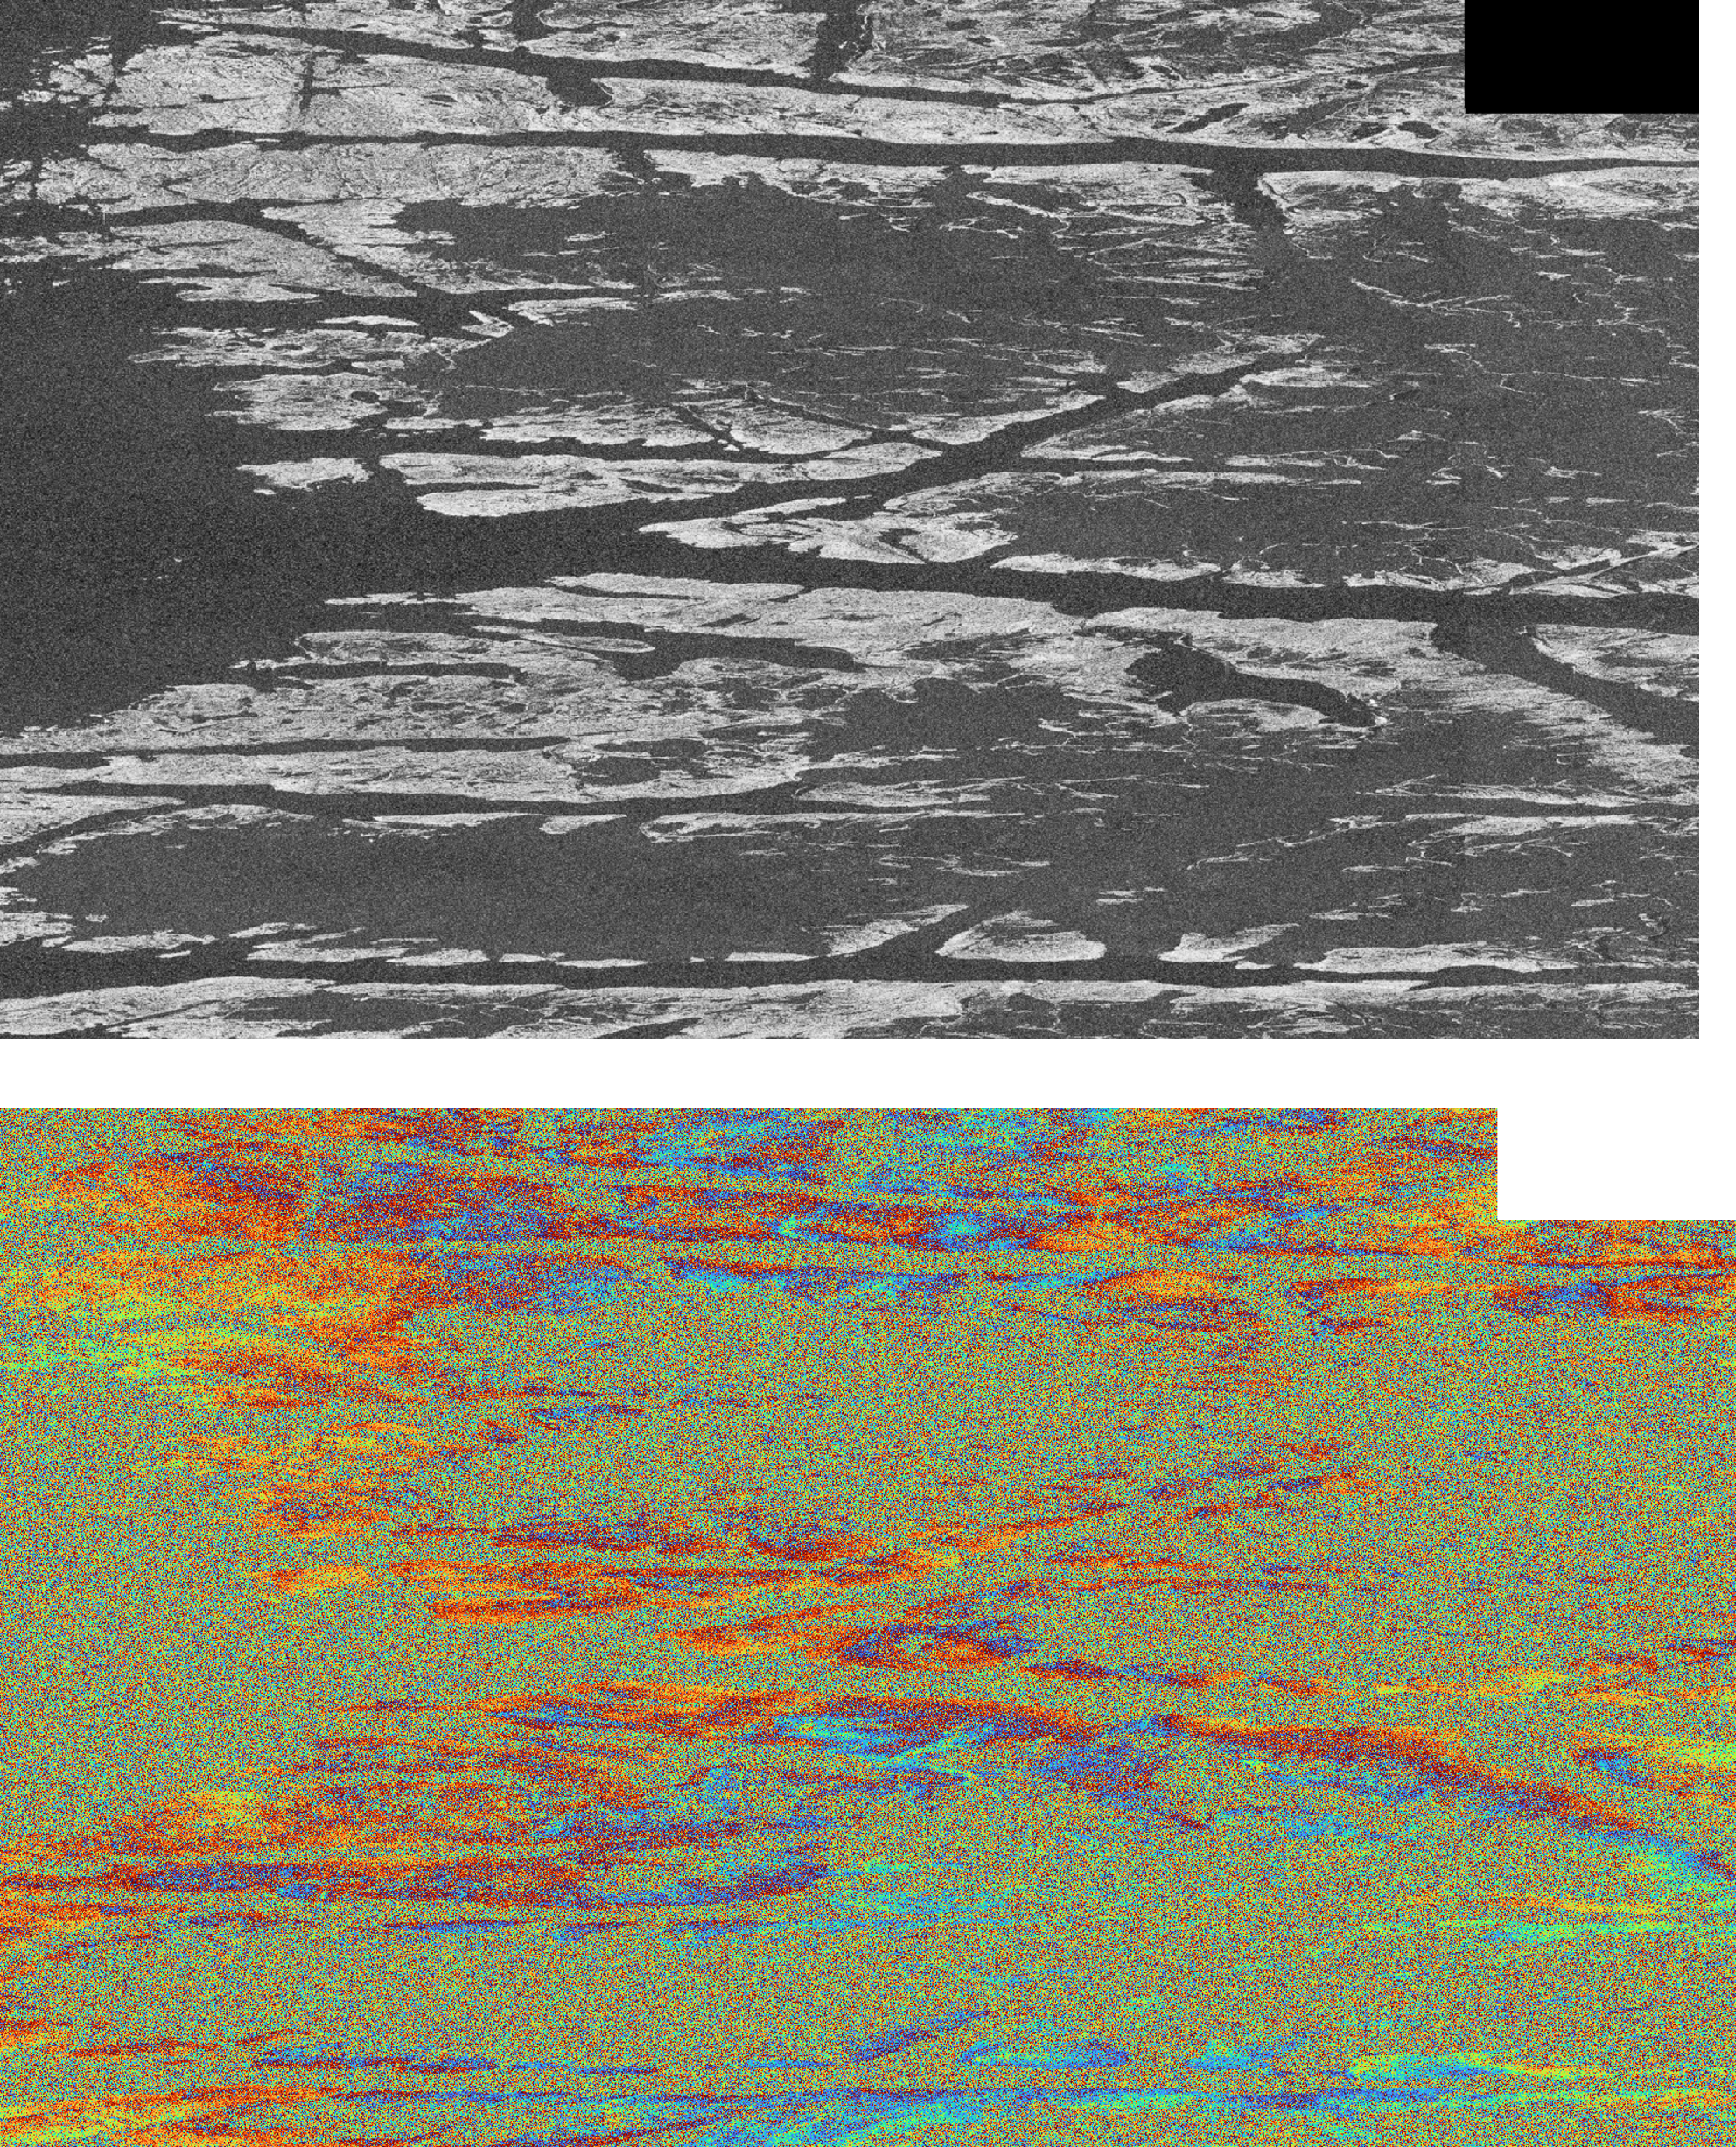
\includegraphics[width=0.9\textwidth]{Figures/strip_eq/cohe_phase_maps.png}
\caption{Interferometric coherence (top) and interferometric phase (bottom) maps derived from two \acs{stripeq} Sentinel-1 \acs{iw} products over Greenland. The input \acs{cslc} data were first co-registered using (\acs{esd}) and then independently mosaicked. The two maps exhibit seamless continuity across both burst and subswath boundaries. A slight increase in coherence in the second subswath is visible due to a higher oversampling factor, which enhances pixel-to-pixel correlation}
\label{fig:interf_coh_maps}
\end{figure}


These results confirm the validity of the \acs{stripeq} approach and its suitability for generating phase-consistent, analysis-ready \acs{sar} products from burst-mode acquisitions.

\subsection{Computational performance}
\label{sec:stripeq_computation}

The computational cost associated with the generation of a \acs{stripeq} product from a \acs{cslc} product is primarily driven by the need to meet the strict co-registration accuracy requirements outlined in the previous section. In particular, refining the azimuth alignment through Enhanced Spectral Diversity (\acs{esd}) constitutes the most computationally involved step. The overall processing workflow comprises the following main stages:

\begin{enumerate}
\item \textbf{Co-registration refinement via \acs{esd}.} For each pair of consecutive bursts within the same sub-swath, the \acs{esd} phase must be computed using only the overlap region. The \acs{esd} phase for each pixel in the overlap area is estimated as:
\begin{equation}
\phi_{ESD}^i(az, rg) = \arg\left((m_{i} \cdot s_{i}^{}) \cdot (m_{i+1} \cdot s_{i+1}^{})\right)
\label{eq:esd_phase}
\end{equation}
where $m_i$ and $s_i$ denote the master and slave complex samples, respectively, and $(i, i+1)$ refers to adjacent bursts. The coherence of the $i$-th burst is also calculated over the same overlap area and used as a weight in the estimation of $\phi_{ESD}^i$, which represents the ESD phase estimate for the $i$-th overlap region (i.e., the region shared by burst pair $(i, i+1)$).

\item \textbf{Phase-to-shift conversion.} All $\phi_{ESD}^i$ values computed in the previous step are aggregated across all burst pairs to estimate the residual azimuth shift. In the simplest case, this is done by averaging the phase values $\phi_{ESD}^i$, although more accurate estimation models can also be applied \citep{Martínez2016}. The computational cost of this step is minimal and can be considered negligible.

\item \textbf{Azimuth shift correction.} Each burst of the slave image is corrected in azimuth based on the estimated residual shift. Given that the residual azimuth error is typically close to a constant, this operation can be efficiently implemented using frequency-domain techniques (e.g., applying a phase ramp via FFT), resulting in low computational overhead compared to spatial-domain sinc-based interpolation. If this step cannot be implemented using a frequency-domain techniques, we need to consider for this step the same computational cost described in the \acs{cslc} product section. In particual, for every output pixel the interpolation algorithm evaluates a finite two-dimensional sinc kernel apodised by a Kaiser window.  
With an \(M\times N\) kernel the operation count is \(MN\) multiplications plus \(MN-1\) additions per pixel; high-fidelity implementations typically use a kernel of at least \(11\times11\). 

\item \textbf{Burst mosaicking.} The final step involves stitching the finely co-registered bursts together. This mosaicking operation is computationally inexpensive and primarily limited by I/O performance, as it entails reading, merging, and writing the corrected burst data.
\end{enumerate}

Overall, the dominant computational burden lies in the \acs{esd}-based refinement, particularly in calculating phase and coherence over multiple burst overlap regions. However, the subsequent steps are lightweight, and FFT-based implementations (when possible) help keep the overall processing pipeline efficient and scalable. 

It is worth noting that when the input \acs{cslc} data already meet the required co-registration accuracy—e.g., due to the use of a data-driven co-registration approach—the only step needed to generate the \acs{stripeq} product is the final mosaicking stage. In such cases, the additional computational cost is negligible.

\subsection{Criticalities and weakness}
\label{sec:stripeq_criticalities}


Two different scenarios must be considered regarding the generation of a \acs{stripeq} product from a \acs{cslc} input:

\begin{enumerate}
\item \textbf{Co-registration accuracy is already sufficient.} If the input \acs{cslc} already satisfies the co-registration accuracy requirements necessary for generating a valid \acs{stripeq} product---such as when a data-driven approach has been used during the co-registration process---and no co-registration refinement is required, no additional criticalities specific to the Stripmap-equivalent generation step are introduced. In this case, the process is limited to burst mosaicking, which is straightforward.

\item \textbf{Co-registration refinement is required.} If the input \acs{cslc} does not meet the required accuracy---e.g., in the case of Sentinel-1 data co-registered using only orbital information and a DEM---then the azimuth refinement described in the previous section must be applied. In this scenario, the generation of a \acs{stripeq} product inherits the same criticalities already discussed for the \acs{cslc} product, particularly the dependency on a consistently selected master image. This includes the need for robust master selection strategies and, in some cases, the updating of the reference master over time, both of which may introduce additional complexity into the processing workflow.
\end{enumerate}
